
\section{Introduction}                % Print a "chapter" heading

The last decade has witnessed an experimental revolution in data science and machine learning, epitomised by deep learning methods. Indeed, many high-dimensional learning tasks previously thought to be beyond reach -- such as computer vision, playing Go, or protein folding -- are in fact feasible with appropriate computational scale.  
%
 Remarkably, the essence of deep learning is built from two simple algorithmic principles: 
 first, the notion of representation or \emph{feature learning}, whereby adapted, often hierarchical, features  capture the appropriate notion of regularity for each task, and second, learning by local gradient-descent, typically implemented as {\em backpropagation}. %, such as gradient descent. 

While learning generic functions in high dimensions is a cursed estimation problem, most tasks of interest are not generic, and come with essential pre-defined regularities arising from the underlying low-dimensionality and structure of the physical world. This text is concerned with exposing these regularities through unified geometric principles that can be applied throughout a wide spectrum of applications. 

Exploiting the known symmetries of a large system is a powerful and classical remedy against the curse of dimensionality, and forms the basis of most physical theories. Deep learning systems are no exception, and since the early days researchers have adapted neural networks to exploit the low-dimensional geometry arising from physical measurements, e.g. grids in images, sequences in time-series, or position and momentum in molecules, and their associated symmetries, such as translation or rotation. 
Throughout our exposition, we will describe these models, as well as many others, as natural instances of the same underlying principle of geometric regularity.%stability. 

Such a `geometric unification' endeavour 
in the spirit of the Erlangen Program 
%--our own Erlangen Program
%\marginnote{We are mindful that the risk of flashy buzzwords such as {\em The Hilbert Problems of X} or {\em Erlangen Program of Y} inevitably implies the irreverent analogy between ourselves and the aforementioned giants. Our only intent here is to draw inspiration from Klein's approach -- {\em ergo, parce nobis, benevole lector!}
%} -- 
serves a dual purpose: on one hand, it provides a common mathematical framework to study the most successful neural network architectures, such as CNNs, RNNs, GNNs, 
and Transformers. On the other, it gives a constructive procedure to incorporate prior physical knowledge into neural architectures %, an essential ingredient to improve the sample efficiency of data-driven methods into computational sciences 
and provide principled way to build future architectures yet to be invented.  

Before proceeding, it is worth noting that our work concerns \emph{representation learning architectures}  and exploiting the symmetries of data therein. The many exciting \emph{pipelines} where such representations may be used (such as self-supervised learning, generative modelling, or reinforcement learning) are \emph{not} our central focus\marginnote{The same applies for techniques used for \emph{optimising} or \emph{regularising} our architectures, such as Adam \citep{kingma2014adam}, dropout \citep{srivastava2014dropout} or batch normalisation \citep{ioffe2015batch}.}. Hence, we will not review in depth influential neural pipelines such as variational autoencoders \citep{kingma2013auto}, generative adversarial networks \citep{goodfellow2014generative}, normalising flows  \citep{rezende2015variational}, deep Q-networks \citep{mnih2015human}, proximal policy optimisation \citep{schulman2017proximal}, or deep mutual information maximisation \citep{hjelm2018learning}. That being said, we believe that the principles we will focus on are of significant importance in all of these areas.
%having good foundations on exploiting the geometry of data will lead to successes when the resulting neural architectures are plugged into any of the above pipelines.

Further, while we have attempted to cast a reasonably wide net in order to illustrate the power of our geometric blueprint, our work does not attempt to accurately summarise the \emph{entire} existing wealth of research on Geometric Deep Learning. Rather, we study several well-known architectures in-depth in order to demonstrate the principles and ground them in existing research, with the hope that we have left sufficient references for the reader to meaningfully apply these principles to any future geometric deep architecture they encounter or devise.

%\raggedbottom
\section{Learning in High Dimensions}

%\textbf{[Summarise this section into the main elements here, with less formality]}


% Main points to illustrate:
% \begin{itemize}
%     \item Modern High-dimensional learning as interpolation. Choosing regularity prior for interpolant in high-dimensions? 
%     \item In low-dimensions, we have good notions of regularity (Sobolev, Holder, etc. ). 
%     \item These can be extended to high-dimensions using reproducing kernel hilbert spaces, or Lipschitz classes. They all suffer from a curse of dimensionality, consequence of the fact that no structural assumptions are made on the data domain. 
%     \item Functions parametrised as neural networks? 
    
% \end{itemize}

Supervised machine learning, in its simplest formalisation, considers a set of $N$ observations $\gD=\{(x_i, y_i)\}_{i=1}^{ N}$ drawn \emph{i.i.d.} 
from an underlying data distribution $P$ defined over $\gX \times \gY$, where $\gX$ and $\gY$ are respectively the data and the label domains. The defining feature in this setup is that $\gX$ is a {\em high-dimensional space}: one typically assumes $\gX= \R^d$ to be a  Euclidean space  of large dimension $d$.

%In our context, however, $\gX$ will often take a more structured form, such as the space of functions $\gX(\Omega) = \{ x: \Omega \to \R \}$ defined over a low-dimensional domain $\Omega$, which can be a geometric object such as a grid, manifold, or a graph. 

Let us further assume that the labels $y$ are generated by an unknown function $f$, such that $y_i = f(x_i)$, 
and the learning problem reduces to estimating the function $f$ using a parametrised function class $\gF=\{ f_{\thetab \in \Theta}\}$. Neural networks are a common realisation of such parametric function classes, in which case $\thetab \in \Theta$ corresponds to the network weights. 
%e.g. to the weights of a neural network. 
In this idealised setup, there is no noise in the labels, and modern deep learning systems typically operate in the so-called \emph{interpolating regime}, where the estimated $\tilde{f} \in \gF$ satisfies $\tilde{f}(x_i) = f(x_i)$ for all $i=1,\hdots, N$.  
The performance of a learning algorithm is measured in terms of the \emph{expected performance} \marginnote{Statistical learning theory is concerned with more refined notions of generalisation based on {\em concentration inequalities}; we will review some of these in future work.} on new samples drawn from ${P}$, using some {\em loss} $L(\cdot,\cdot)$ 
$$\gR(\tilde{f}):= \mathbb{E}_{P}\,\, L(\tilde{f}(x), f(x)),$$
%
with the squared-loss $L(y,y')=\frac{1}{2}|y-y'|^2$ being among the most commonly used ones.  


A successful learning scheme thus needs to encode the appropriate notion of regularity or  \emph{inductive bias} for $f$, imposed through the construction of the function class $\mathcal{F}$ and the use of {\em regularisation}. We briefly introduce this concept in the following section. %, and will explore it in detail in follow-up work. 


\subsection{Inductive Bias via Function Regularity}
\label{sec:inductive}


Modern machine learning operates with large, high-quality datasets, which, together with appropriate computational resources, motivate the design of rich function classes $\gF$ with the capacity to interpolate such large data. 
%
This 
%non-parametric % Taco: can we really call this "non-parametric"? It's just a very large parametric function space, no?
mindset plays well with neural networks, since even the simplest choices of architecture yields a {\em dense} class of functions.\marginnote{A set $\mathcal{A}\subset \mathcal{X}$ is said to be {\em dense} in $\mathcal{X}$ if its closure
$$
\mathcal{A}\cup \{ \displaystyle \lim_{i\rightarrow \infty} a_i : a_i \in \mathcal{A}\} = \mathcal{X}.
$$ 
This implies that any point in $\mathcal{X}$ is arbitrarily close to a point in $\mathcal{A}$. A typical Universal Approximation result shows that the class of functions represented e.g. by a two-layer perceptron, $f(\mathbf{x}) = \mathbf{c}^\top\mathrm{sign}(\mathbf{A}\mathbf{x}+\mathbf{b})$ is dense in the space of continuous functions on $\mathbb{R}^d$. 
} 
%
The capacity to approximate almost arbitrary functions
%\marginnote{More precisely, Borel-measurable. } 
is the subject of various \emph{Universal Approximation Theorems}; several such results were proved and popularised in the 1990s by applied mathematicians and computer scientists (see e.g. \cite{cybenko1989approximation,hornik1991approximation,barron1993universal,leshno1993multilayer,maiorov1999best,pinkus1999approximation}). 
%(Barron, Meir, Maiorov, Pinkus, Cybenko, Hornik, etc.) 

\begin{figure}[h!]
    \centering
    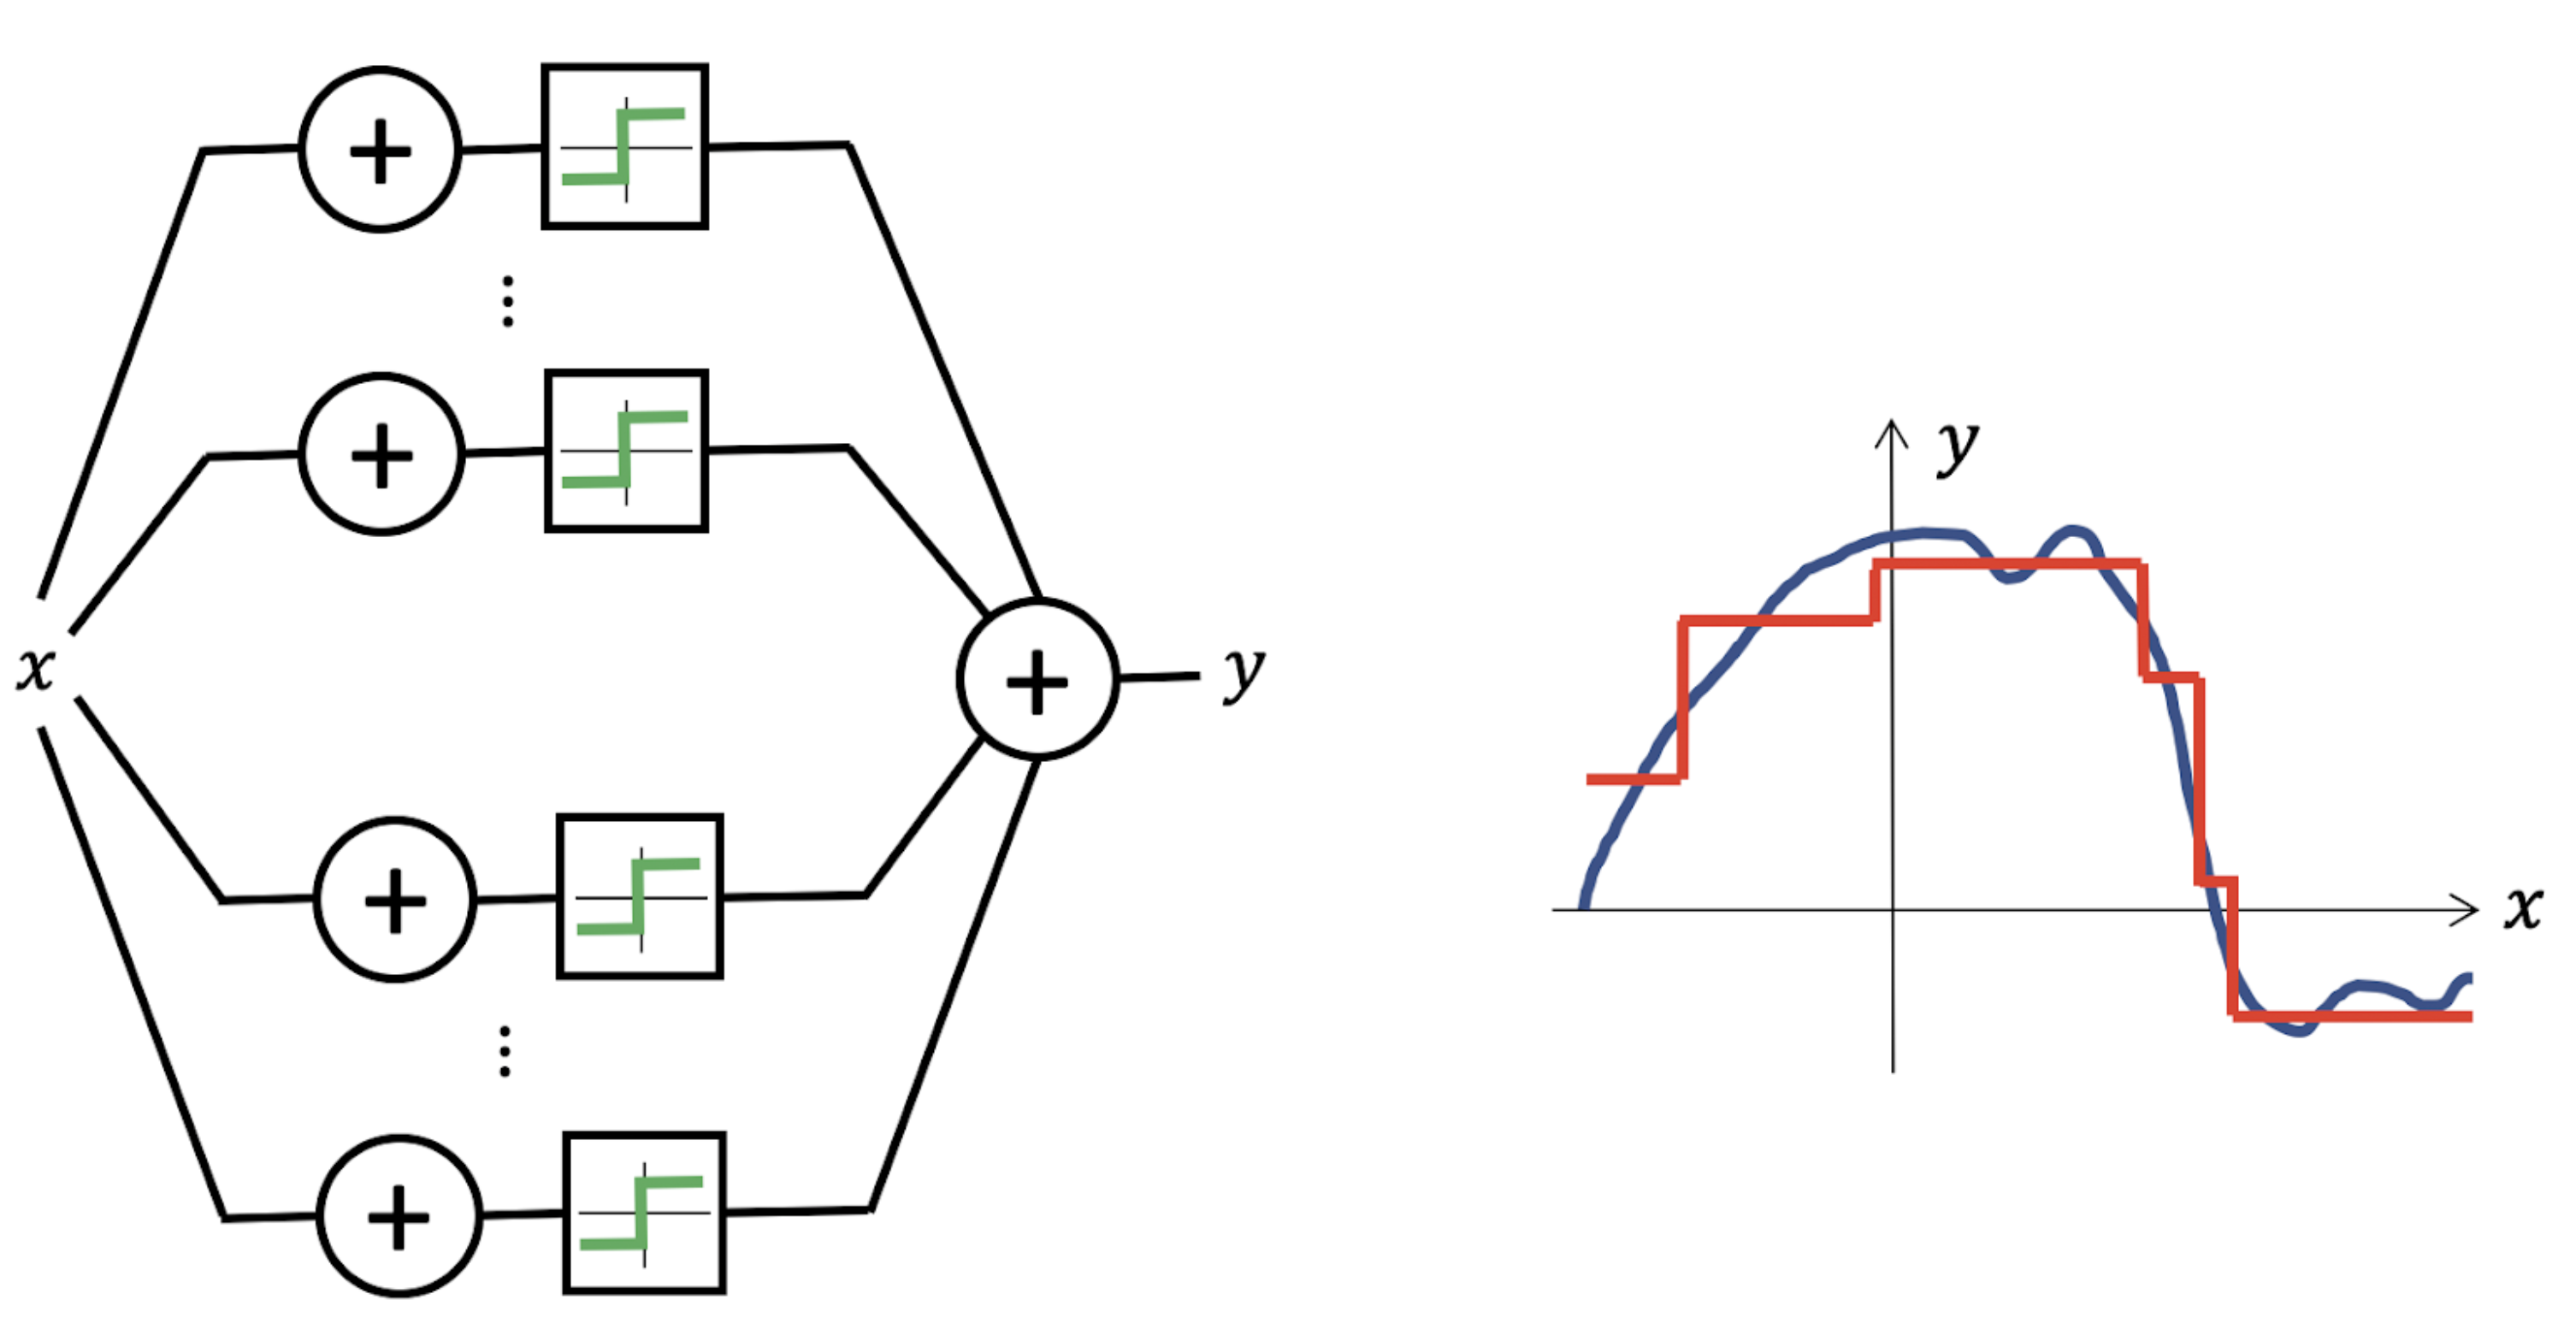
\includegraphics[width=1\linewidth]{figures/ua_mlp.png}
    \caption{Multilayer Perceptrons \citep{rosenblatt1958perceptron}, the simplest feed-forward neural networks, are universal approximators: with just one hidden layer, they can represent combinations of step functions, allowing to approximate any continuous function with arbitrary precision.}
    \label{fig:ua_mlp}
\end{figure}%


%\michael{Show an intuitive example of MLP approximating step functions}


Universal Approximation, however, does not imply an {\em absence} of inductive bias. Given a hypothesis space $\gF$ with universal approximation, we can define a complexity measure $c: \gF \to \R_{+}$ and redefine our interpolation problem as 
$$
\tilde{f} \in \arg\min_{g \in \gF} c(g) \quad \mathrm{s.t.} \quad g(x_i) = f(x_i)  \quad \mathrm{for} \,\,\, i=1, \hdots, N,
$$
i.e., we are looking for the most regular functions within our hypothesis class. 
%
For standard function spaces, this complexity measure can be defined as a {\em norm},\marginnote{
%A {\em norm} is a non-negative function $\| \cdot \|$ on a vector space that is {\em homogeneous} $\| \alpha x \| = |\alpha| \| x\|$, {\em subadditive} $\|x+y \| \leq \|x\| + \|y\|$ and {\em positive-definite} $\|x\|=0 \Rightarrow x=0$. 
Informally, a norm $\|x\|$ can be regarded as a ``length'' of vector $x$. 
A {\em Banach space} is a complete vector space equipped with a norm. 
} making $\gF$ a {\em Banach space} and allowing to leverage a plethora of theoretical results in functional analysis. 
%
In low dimensions, splines are a workhorse for function approximation. They can be formulated as above, with a norm capturing 
the classical notion of smoothness, such as the squared-norm of second-derivatives $\int_{-\infty}^{+\infty} |f''(x)|^2 \mathrm{d}x$ for cubic splines. 

%\michael{Notation: change complexity from $\gamma$ to $c$ (which we used for Dirichlet)?}


In the case of neural networks,  the complexity measure $c$ can be expressed in terms of the network weights, i.e. $c(f_{\boldsymbol{\theta}}) = {c}(\boldsymbol{\theta})$.
%
The $L_2$-norm of the network weights, known as \emph{weight decay}, or the so-called \emph{path-norm} \citep{neyshabur2015norm} are popular choices in deep learning literature.  
%\michael{I suggest we give concrete examples here, e.g. sparsity-inducing regularization and low-dimensional projections}
%
%
From a Bayesian perspective, such complexity measures can also be interpreted as the negative log of the prior for the function of interest. More generally, this complexity can be enforced \emph{explicitly} by incorporating it into the empirical loss (resulting in the so-called Structural Risk Minimisation), or \emph{implicitly}, as a result of a certain optimisation scheme. For example, it is well-known that gradient-descent on an under-determined least-squares objective will choose interpolating solutions with minimal $L_2$ norm. The extension of such implicit regularisation results to modern neural networks is the subject of current studies (see e.g. \cite{blanc2020implicit, shamir2020implicit, razin2020implicit, gunasekar2017implicit}).   
All in all, a natural question arises: how to define effective priors that capture the expected regularities and complexities of real-world prediction tasks? 
%We will address this question in Chapter ??




\subsection{The Curse of Dimensionality}

While interpolation in low-dimensions %$\gX = \R^d$ 
(with $d=1,2$ or $3$) is a classic signal processing task with very precise mathematical control of estimation errors using increasingly sophisticated regularity classes (such as spline interpolants, wavelets, curvelets, or ridgelets), the situation for high-dimensional problems is entirely different. 
%

% \begin{figure}[h!]
%     \centering
%     %\includegraphics[width=0.3\linewidth]{figures/curseofdim1.pdf}
%     \caption{An $\epsilon$-net of a  $d$-dimensional Euclidean domain of diameter $1$ grows exponentially as $\epsilon^{-d}$. }
%     \label{fig:curseofdim}
% \end{figure}%

%\michael{We need to clean up notation: in ML problems our main object is $f(x)$ where $x$ is the input, e.g. an image. It has its own structure, being in own turn a signal on the domain, $x(u)$.}

In order to convey the essence of the idea, let us consider a classical notion of regularity that can be easily extended to high dimensions: 1-Lipschitz- functions $f:\mathcal{X} \to \R$, i.e. functions satisfying  $|f(x) - f(x')| \leq \|x - x'\|$ for all $x, x' \in \mathcal{X}$. This hypothesis only asks the target function to be \emph{locally} smooth, i.e., if we perturb the input $x$ slightly (as measured by the norm $\|x - x'\|$), the output $f(x)$ is not allowed to change much. %\michael{Lets avoid confusion and use $\mathcal{X}$ rather than $\Omega$}
%\marginnote{The number of protons in the observable universe, known as the {\em Eddington number}, is currently estimated at $\sim 10^{80}$.}
If our only knowledge of the target function $f$ is that it is $1$-Lipschitz, how many observations do we expect to require to ensure that our estimate $\tilde{f}$ will be close to $f$? 
Figure \ref{fig:curseofdim} reveals that the general answer is necessarily exponential in the dimension $d$, signaling that the Lipschitz class grows `too quickly' as the input dimension increases: in many applications with even modest dimension $d$, the number of samples would be bigger than the number of atoms in the universe.
 The situation is not better if one replaces the Lipschitz class by a global smoothness hypothesis, such as the Sobolev Class $\gH^{s}(\Omega_d)$\marginnote{A function $f$ is in the {\em Sobolev class} $\gH^{s}(\Omega_d)$ if $f \in L^2(\Omega_d)$ and the generalised $s$-th order derivative is square-integrable: $\int |\omega|^{2s+1} |\hat{f}(\omega)|^2 d\omega < \infty$, where 
$\hat{f}$ is the Fourier transform of $f$; see Section~\ref{sec:grids_euclidean}. 
}. Indeed, classic results \citep{tsybakov2008introduction} establish a minimax rate of approximation and learning for the Sobolev class of the order $\epsilon^{-d/s}$, showing that the extra smoothness assumptions on $f$ only improve the statistical picture when $s \propto d$, an unrealistic assumption in practice. 

% on the one hand, `globally' smooth functions, with $s$-order derivatives \marginnote{The \emph{Sobolev} class defines  }

% In fact, even though we can extend the above `classic' functional spaces to arbitrary dimensions, they suffer from the so-called \emph{curse of dimensionality}. In essence, in order to obtain an expected generalization error $\mathbb{E}_{x\sim \mathbb{P}} | \tilde{f}(x) - f(x)| \leq \epsilon$, such regularity hypotheses require an order of $\epsilon^{-d}$ observations, signalling an impossibility of efficient learning : in many applications with even modest dimension $d$, the number of samples would be bigger than the number of atoms in the universe.
% \marginnote{The number of protons in the observable universe, known as the Eddington number, is currently estimated at $\sim 10^{80}$.}

\begin{figure}[h!]
    \centering
%    \includegraphics[width=0.45\linewidth]{figures/curseofdim4.pdf} 
 %       \includegraphics[width=0.45\linewidth]{figures/curseofdim2.pdf}
       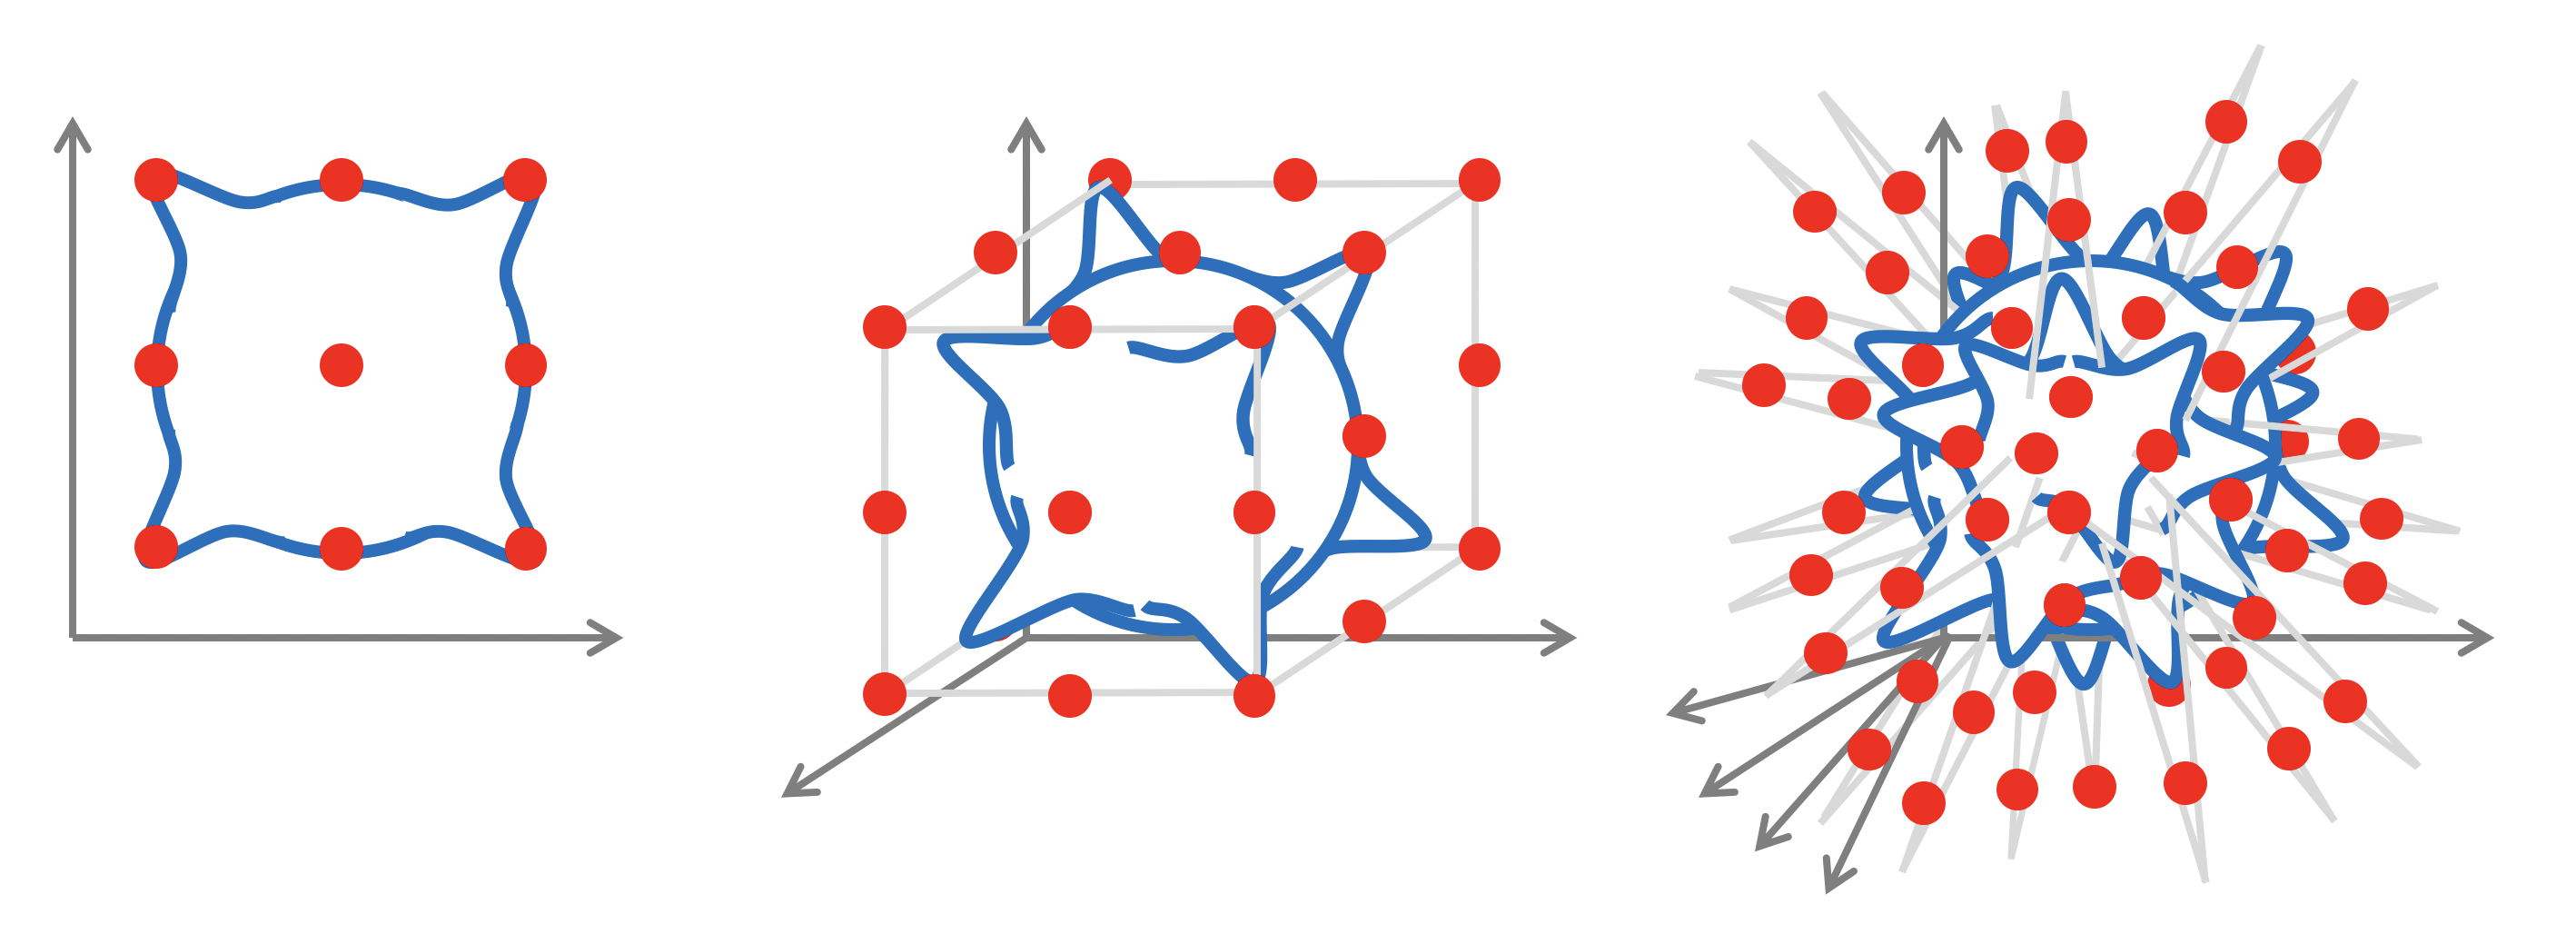
\includegraphics[width=\linewidth]{figures/blobs.png} 
    \caption{We consider a Lipschitz function $f(x) = \sum_{j=1}^{2^d} z_j \phi(x-x_j)$ where $z_j=\pm 1$, $x_j \in \R^d$ is placed in each quadrant, and $\phi$ a locally supported Lipschitz `bump'. Unless we observe the function in most of the $2^d$ quadrants, we will incur in a constant error in predicting it. This simple geometric argument can be formalised through the notion of \emph{Maximum Discrepancy} \citep{von2004distance}, defined for the Lipschitz class as $\kappa(d)=\mathbb{E}_{x,x'} \sup_{f \in \mathrm{Lip}(1)} \left| \frac{1}{N}\sum_{l} f(x_l) - \frac{1}{N}\sum_{l} f(x'_l) \right| \simeq N^{-1/d}$, which measures the largest expected discrepancy between two independent $N$-sample expectations. Ensuring that $\kappa(d) \simeq \epsilon$ requires $N = \Theta(\epsilon^{-d})$; the corresponding sample $\{x_l\}_l$ defines an $\epsilon$-net of the domain. For a $d$-dimensional Euclidean domain of diameter $1$, its size grows exponentially as $\epsilon^{-d}$.}
    \label{fig:curseofdim}
\end{figure}


%\michael{\bf [MB: INSERT FIGURE and explain the curse of dimensionality as a geometric phenomenon using the volume of inscribed unit ball]}


%\michael{\bf [MB: General comment: in order not to interrupt the flow, we can have self-contained figures with long captions or `inserts' explaining important concepts. We had it in our Signal Processing Magazine paper and it was a very good idea
%}

%\joan{Agreed. The Curse of Dimensonality could be one such insert, with a panel with (i) a figure that displays the exponential dependence of epsilon-grids wrt dimension, and caption. TODO JOAN}

Fully-connected neural networks define function spaces that enable more flexible notions of regularity, obtained by considering complexity functions $c$ on their weights. In particular, by choosing a sparsity-promoting regularisation, they have the ability to break this curse of dimensionality \citep{bach2017breaking}. However, this comes at the expense of making strong assumptions on the nature of the target function $f$, such as that $f$ depends on a collection of low-dimensional projections of the input (see Figure \ref{fig:curseofdim2}).
%\michael{\bf [MB: not sure I understand this part. Isn't there a universal approximation result?]} \joan{I further clarified}
In most real-world applications (such as computer vision, speech analysis, physics, or  chemistry), functions of interest %$f$ 
tend to exhibits complex long-range correlations that cannot be expressed with low-dimensional projections (Figure \ref{fig:curseofdim2}), making this hypothesis unrealistic.  
It is thus necessary to define an alternative source of regularity, by exploiting the spatial structure of the physical domain and the geometric priors of $f$, as we describe in the next Section~\ref{sec:geom_priors}. 

\begin{figure}[htbp]
    \centering
%    \includegraphics[width=0.45\linewidth]{figures/curseofdim5.pdf} 
%    \includegraphics[width=0.45\linewidth]{figures/mnistm.pdf} %
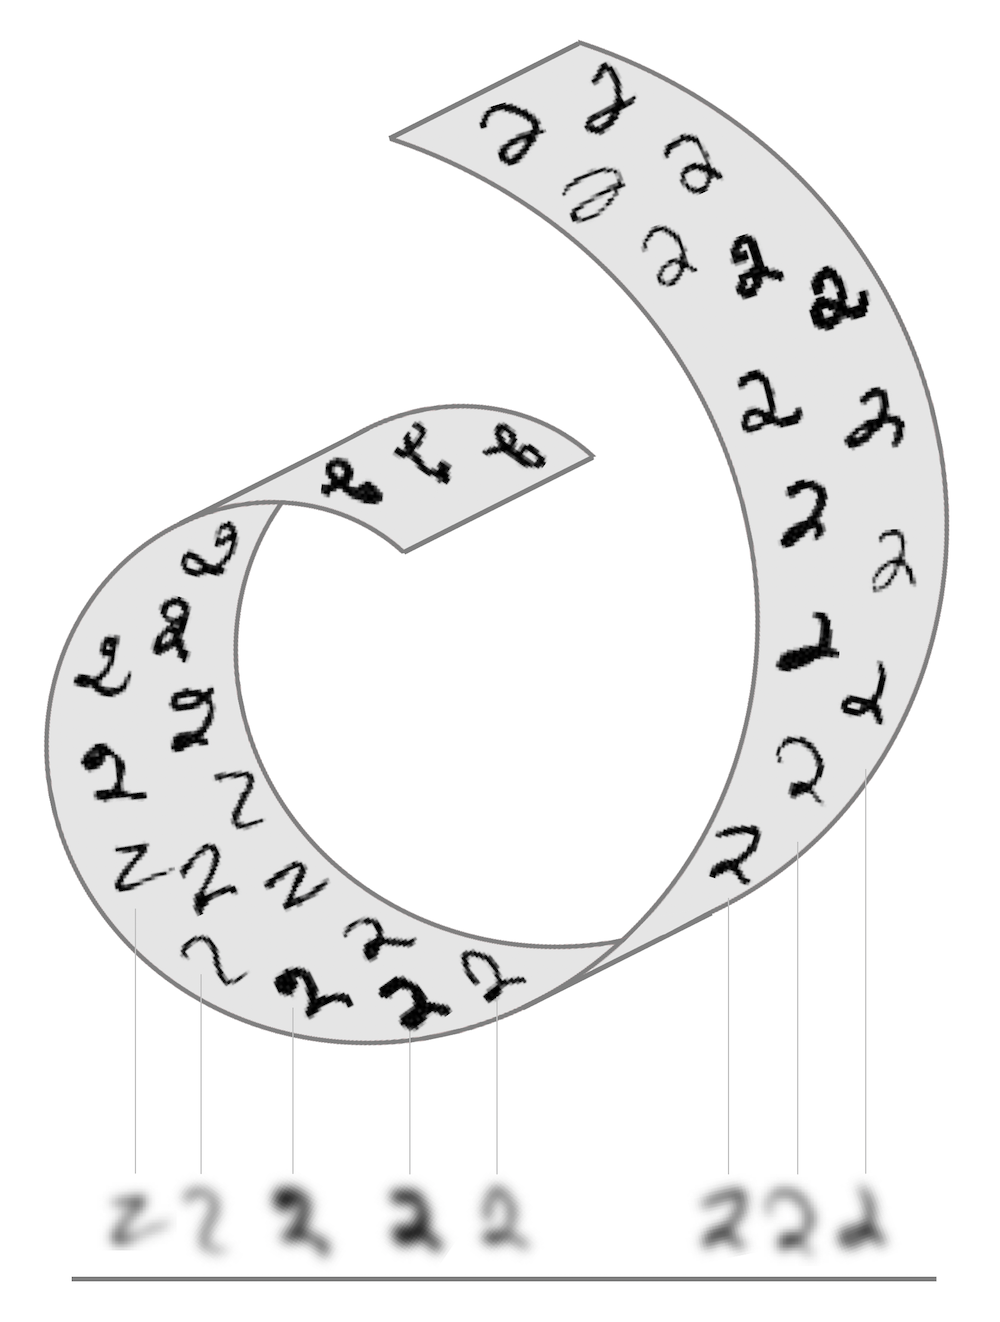
\includegraphics[width=0.6\linewidth]{figures/mnist.png}
    \caption{%\michael{Lets not use $\Omega$ here but $\mathcal{X}$ as the domain of $f$} 
    If the unknown function $f$ %:\gX \to \R$ 
    is presumed to be well approximated as $f(\mathbf{x}) \approx g(\mathbf{A}\mathbf{x})$ for some unknown $\mathbf{A} \in \mathbb{R}^{k \times d}$ with $k \ll d$, then shallow neural networks can capture this inductive bias, see e.g.  \cite{bach2017breaking}. In typical applications, such dependency on low-dimensional projections is unrealistic, as illustrated in this example: a low-pass filter projects the input images to a low-dimensional subspace; while it conveys most of the semantics, substantial information is lost.%\michael{Joan: why not to show the Swiss-roll surface?} \joan{Yes, we can use it to replace the sketch in the left. }
    % Taco: is the blurred MNIST really a good example? I guess that if we used a PCA projection we could keep >98% of the variance with only a few components for this dataset. But perhaps for natural images this is no longer true..
    }
    \label{fig:curseofdim2}
\end{figure}


\newpage
\section{Geometric Priors}
\label{sec:geom_priors}
Modern data analysis is synonymous with high-dimensional learning.  
While the simple arguments of Section~\ref{sec:inductive} reveal the impossibility of learning 
from generic high-dimensional data as a result of the curse of dimensionality, 
there is hope for physically-structured data, where we can employ two fundamental principles: {\em symmetry} and {\em scale separation}. 
In the settings considered in this text, this additional structure will usually come from the structure of the domain underlying the input signals: 
we will assume that our machine learning system operates on \emph{signals} (functions) on some domain $\Omega$. 
%
While in many cases linear combinations of points on $\Omega$ is not well-defined\marginnote{$\Omega$ must be a vector space in order for an expression $\alpha u + \beta v$ to make sense.}, we can linearly combine signals on it, i.e., the space of signals forms a vector space. 
Moreover, since we can define an inner product between signals, this space is a {\em Hilbert space}.

\begin{tcolorbox}[width=\linewidth,
                  boxsep=0pt,
                  left=7.5pt,
                  right=7.5pt,
                  top=7.5pt,
                  bottom=7.5pt,
                  arc=0pt,
                  boxrule=0pt,toprule=0pt,
                  colback=boxgray,
                  ]%%

The space of $\mathcal{C}$-valued signals on $\Omega$ 
\marginnote{When $\Omega$ has some additional structure, we may further restrict the kinds of signals in $\mathcal{X}(\Omega, \mathcal{C})$. For example, when $\Omega$ is a smooth manifold, we may require the signals to be smooth. 
Whenever possible, we will omit the range $\mathcal{C}$ for brevity. 
} %can impose smoothness on the signals.}% For instance, when $\Omega$ is a smooth manifold we may require signals in $\mathcal{X}(\Omega, \mathcal{C})$ to be smooth.}
(for $\Omega$ a set, possibly with additional structure, and $\mathcal{C}$ a vector space, whose dimensions are called \emph{channels}) 
\begin{equation}
    \mathcal{X}(\Omega, \mathcal{C}) = \{ x : \Omega \rightarrow \mathcal{C} \}
\end{equation}
%
is a function space that has a vector space structure. 
%In particular, it satisfies the distributivity property 
Addition and scalar multiplication of signals is defined as:
\begin{equation*}
    (\alpha x + \beta y)(u) = \alpha x(u) + \beta y(u) \quad \text{for all} \quad u\in \Omega,
\end{equation*}
with real scalars $\alpha, \beta$. % are vectors, and $u \in \Omega$.
%
Given an inner product $\langle v, w \rangle_\mathcal{C}$ on $\mathcal{C}$ and a measure\marginnote{When the domain $\Omega$ is discrete, $\mu$ can be chosen as the {\em counting measure}, in which case the integral becomes a sum. In the following, we will omit the measure and use $\mathrm{d}u$ for brevity.  } $\mu$ on $\Omega$ (with respect to which we can define an integral), we can define an inner product on $\mathcal{X}(\Omega, \mathcal{C})$ as 
\begin{equation}
    \langle x, y \rangle = \int_{\Omega} \langle x(u), \, y(u) \rangle_{\mathcal{C}} \; \mathrm{d}\mu(u).
    \label{eqn:innerprod}
\end{equation}
\end{tcolorbox}

%we will assume that $f$ operates on $\mathcal{C}$-valued signals $\mathcal{X}(\Omega, \mathcal{C}) = \{x: \Omega \rightarrow \mathcal{C} \}$, where $\Omega$ is some input domain and $\mathcal{C}$ is a vector space, typically $\mathcal{C} = \R^s$ for a signal with $s$ channels.
%\marginnote{For the sake of simplicity, we will often assume scalar-valued signals, i.e., $s=1$. }
%We note that $\mathcal{X}(\Omega, \mathcal{C})$ is a vector space, with addition and scalar multiplication defined pointwise (i.e. $(f + f')(x) = f(x) + f(x')$ and $(\alpha f)(x) = \alpha f(x)$).

As a typical illustration, take $\Omega = \mathbb{Z}_n\times \mathbb{Z}_n$ to be a two-dimensional $n\times n$ grid, $x$ an RGB image (i.e. a signal $x : \Omega \rightarrow \R^3$), and $f$ a function (such as a single-layer Perceptron) operating on $3n^2$-dimensional inputs. 
%
As we will see in the following with greater detail, the domain $\Omega$ is usually endowed with certain geometric structure and symmetries. %symmetric structure (in our example, rotational and translational symmetry) that is manifested both in signals $x$ defined on this domain as well as in functions $f$ acting on such signals. 
%
Scale separation results from our ability to preserve important characteristics of the signal when transferring it onto a coarser version of the domain (in our example, subsampling the image by coarsening the underlying grid). 


We will show that both principles, to which we will generically refer as {\em geometric priors}, are prominent in most modern deep learning architectures. In the case of images considered above, geometric priors are built into Convolutional Neural Networks (CNNs) in the form of convolutional filters with shared weights (exploiting translational symmetry) and pooling (exploiting scale separation). 
%
Extending these ideas to other domains such as graphs and manifolds and showing how geometric priors emerge from fundamental principles is the main goal of Geometric Deep Learning and the {\em leitmotif} of our text.   



\subsection{Symmetries, Representations, and Invariance}
\label{sec:symmetries}

%Symmetries are a foundational principle of physics, providing a strong constraint on the form of physical laws.
%In the context of machine learning, symmetries also provide key regularity priors that allow to break the curse of dimensionality and enable efficient high-dimensional learning. 

Informally, a {\em symmetry} of an object or system is a transformation that leaves a certain property of said object or system unchanged or {\em invariant}.
Such transformations may be either smooth, continuous, or discrete.
%A canonical example for continuous symmetries in physics is Lagrangian mechanics, which states that the laws of motion are preserved under rigid transformations of the observer's point of view. 
%
Symmetries are ubiquitous in many machine learning tasks.
For example, in computer vision the object category is unchanged by shifts, so shifts are symmetries in the problem of visual object classification.
%one is often interested in classifying  objects in images independently of their position, a setting referred to as {\em translation invariant}. 
%
%classification through translation invariance, or 
In computational chemistry, the task of predicting properties of molecules independently of their orientation in space requires {\em rotational invariance}. 
%
Discrete symmetries emerge naturally when describing particle systems where particles do not have canonical ordering and thus can be arbitrarily permuted, as well as
%through permutations, 
%or also 
in many dynamical systems, via the time-reversal symmetry (such as systems in detailed balance or the Newton's second law of motion). %\marginnote{ADD COMMENT on Newton's law} % may not be necessary imo
%
As we will see in Section~\ref{sec:proto-graphs}, permutation symmetries are also central to the analysis of graph-structured data. % and will be a prominent topic in this book. 

\paragraph{Symmetry groups}
The set of symmetries of an object satisfies a number of properties. 
%which make this set into an algebraic structure called a \emph{symmetry group}.
%Symmetries lend themselves to a rich and powerful mathematical characterization.
%More specifically, the set of symmetries of a given object forms an algebraic object called a symmetry group.
First, symmetries may be combined to obtain new symmetries: if $\fg$ and $\fh$ are two symmetries,
%transformations of a system that leave it unchanged, 
then their  compositions $\fg \circ \fh$ and $\fh \circ \fg$
%\marginnote{From hereon we will denote composition of group elements by $\fg \fh$, leaving out the $\circ$ symbol.}
\marginnote{We will follow the juxtaposition notation convention used in group theory, $\fg \circ \fh = \fg \fh$, which should be read right-to-left: we first apply $\fh$ and then $\fg$. The order is important, as in many cases symmetries are non-commutative. 
%
Readers familiar with Lie groups might be disturbed by our choice to use the Fraktur font to denote group elements, as it is a  common notation of Lie algebras.
} are also symmetries.
The reason is that if both transformations leave the object invariant, then so does the composition of transformations, and hence the composition is also a symmetry.
%\marginnote{This property is called {\em closure} in group theory.} 
Furthermore, symmetries are always invertible, and the inverse is also a symmetry.
%Together with {\em associativity} $(\fg \circ \fh) \circ \ff = \fg \circ (\fh \circ \ff)$ of the composition operation and existence of unique {\em identity} ($\exists!\fe \in \fG$ such that $\fe \circ \fg = \fg \circ \fe = \fe$ for all $\fg \in \fG$) and {\em inverse} (for any $\fg \in \fG$, $\exists! \fg^{-1} \in \fG$ such that $\fg\circ \fg^{-1} = \fg^{-1}\circ \fg = \fe$), it formally defines a group.} 
This shows that the collection of all symmetries form an algebraic object known as a {\em group}. Since these objects will be a centerpiece of the mathematical model of Geometric Deep Learning, they deserve a formal definition and detailed discussion:
%The symmetries of any system thus form a {\em group} with the composition operation, which can be studied with powerful tools from representation theory, algebra and geometry.


%\taco{TODO: Make this into a Definition Box.}


\begin{tcolorbox}[width=\linewidth,
                  boxsep=0pt,
                  left=7.5pt,
                  right=7.5pt,
                  top=7.5pt,
                  bottom=7.5pt,
                  arc=0pt,
                  boxrule=0pt,toprule=0pt,
                  colback=boxgray,
                  ]%%
A {\em group} is a set $\fG$ along with a binary operation $\circ : \fG \times \fG \rightarrow \fG$ called {\em composition} (for brevity, denoted by juxtaposition $\fg \circ \fh = \fg \fh$) 
%for $\fg, \fh \in \fG$, 
satisfying the following axioms: \vspace{3mm}\\
%\begin{enumerate}
    %\item 
    \noindent {\em Associativity:} $(\fg \fh) \fk = \fg (\fh \fk)$ for all $\fg, \fh, \fk \in \fG$.\vspace{2mm}\\
    \noindent  {\em Identity:} there exists a unique $\fe \in \fG$ satisfying $\fe \fg = \fg \fe = \fg$ for all $\fg \in \fG$.\vspace{2mm}\\
    \noindent  {\em Inverse:} For each $\fg \in \fG$ there is a unique inverse $\fg^{-1} \in \fG$ such that $\fg \fg^{-1} = \fg^{-1} \fg = \fe$.\vspace{2mm}\\
    \noindent  {\em Closure:} The group is closed under composition, i.e., for every $\fg, \fh \in \fG$, we have $\fg \fh \ \in \fG$.
%\end{enumerate}

\end{tcolorbox}
Note that \emph{commutativity} is not part of this definition, i.e. we may have $\fg \fh \neq \fh \fg$.
Groups for which $\fg \fh = \fh \fg$ for all $\fg, \fh \in \fG$ are called commutative or {\em Abelian}\marginnote{After the Norwegian mathematician Niels Henrik Abel (1802--1829).}.

Though some groups can be very large and even infinite, they often arise from compositions of just a few elements, called {\em group generators}. Formally, $\mathfrak{G}$ is said to be {\em generated} by a subset $S \subseteq \mathfrak{G}$ (called the group {\em generator}) if every element $\fg \in \fG$ can be written as a finite composition of the elements of $S$ and their inverses. 
%
For instance, the symmetry group of an equilateral triangle (dihedral group $\mathrm{D}_3$) is generated by a $60^\circ$ rotation and a reflection (Figure \ref{fig:group-example-d3-s3}). 
%
The 1D {\em translation group}, which we will discuss in detail in the following, is generated by infinitesimal displacements; this is an example of a {\em Lie group} of differentiable symmetries.\marginnote{Lie groups have a differentiable manifold structure. One such example that  we will study in Section~\ref{sec:groups} is the special orthogonal group $\mathrm{SO}(3)$, which is a 3-dimensional manifold.} 


Note that here we have defined a group as an abstract object, without saying what the group elements \emph{are} (e.g. transformations of some domain), only how they \emph{compose}.
Hence, very different kinds of objects may have the same symmetry group.
For instance, the aforementioned group of rotational and reflection symmetries of a triangle is the same as the group of permutations of a sequence of three elements (we can permute the corners in the triangle in any way using a rotation and reflection -- see Figure \ref{fig:group-example-d3-s3})\marginnote{The diagram shown in Figure \ref{fig:group-example-d3-s3} (where each node is associated with a group element, and each arrow with a generator), is known as the {\em Cayley diagram}.}.

\begin{figure}
    \centering
\raisebox{-0.5\height}{    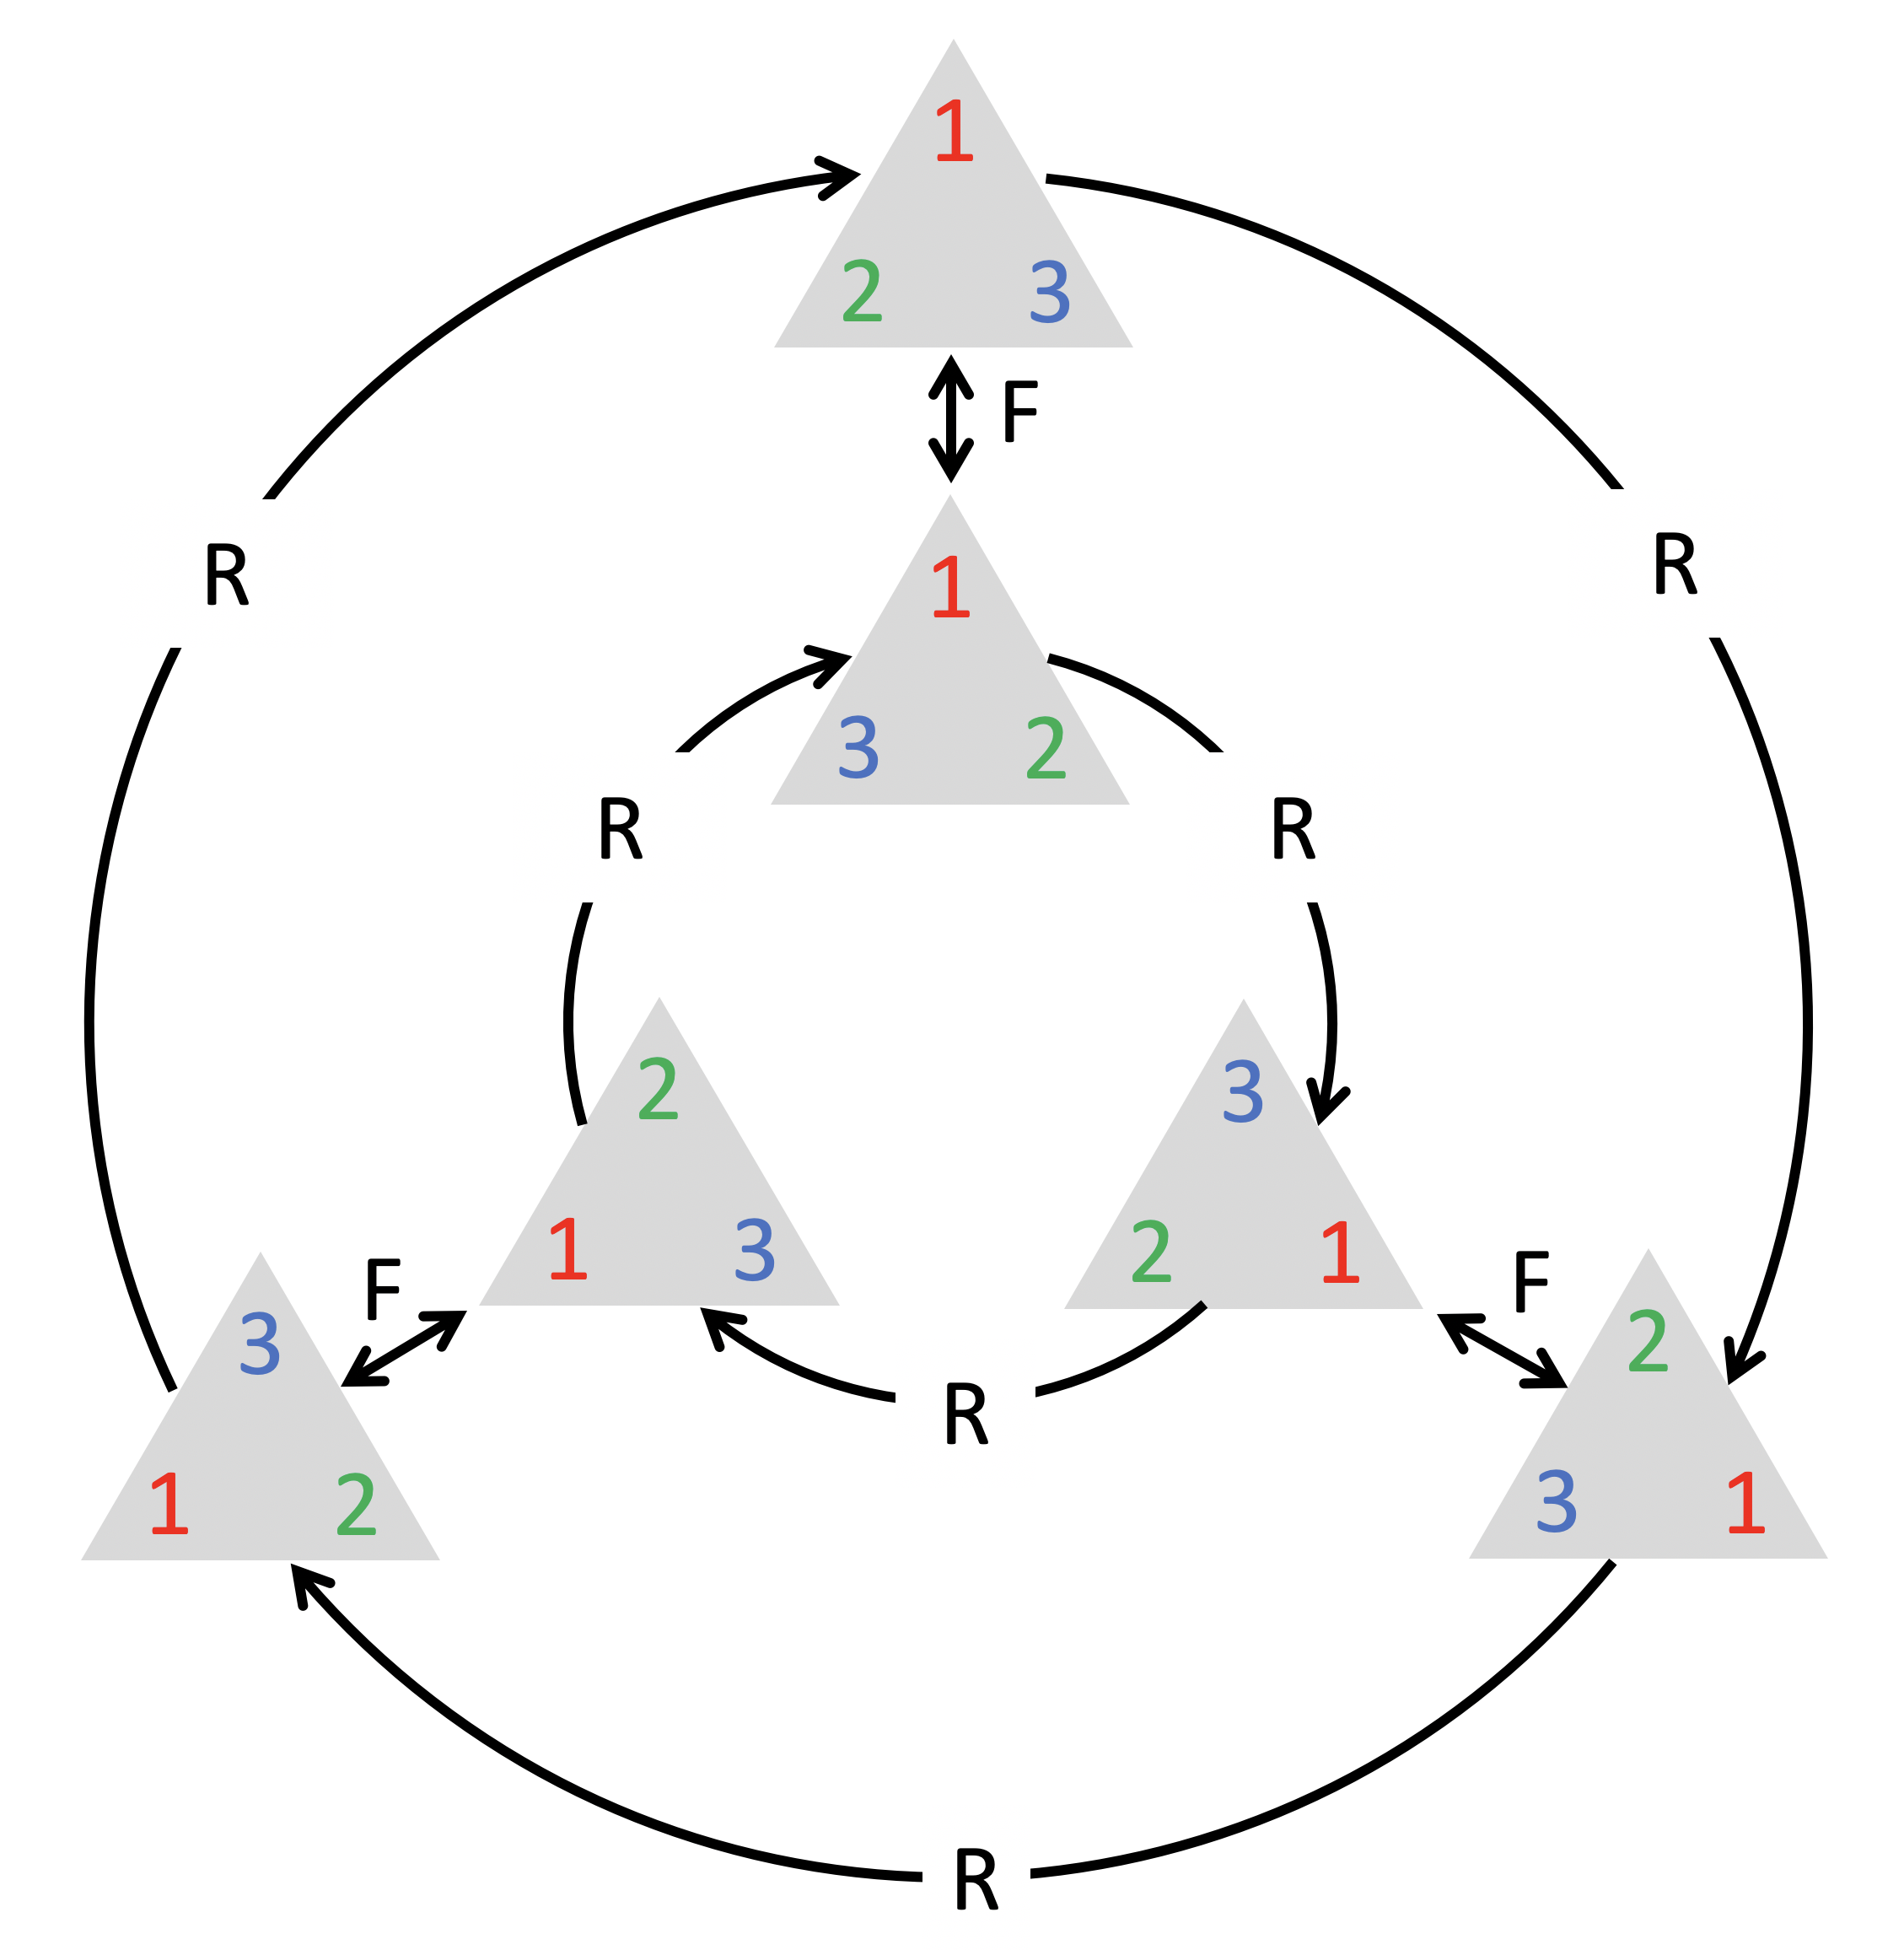
\includegraphics[width=0.45\linewidth]{figures/group_d3.png}
}
    \hspace{2mm}
    \raisebox{-0.5\height}{
        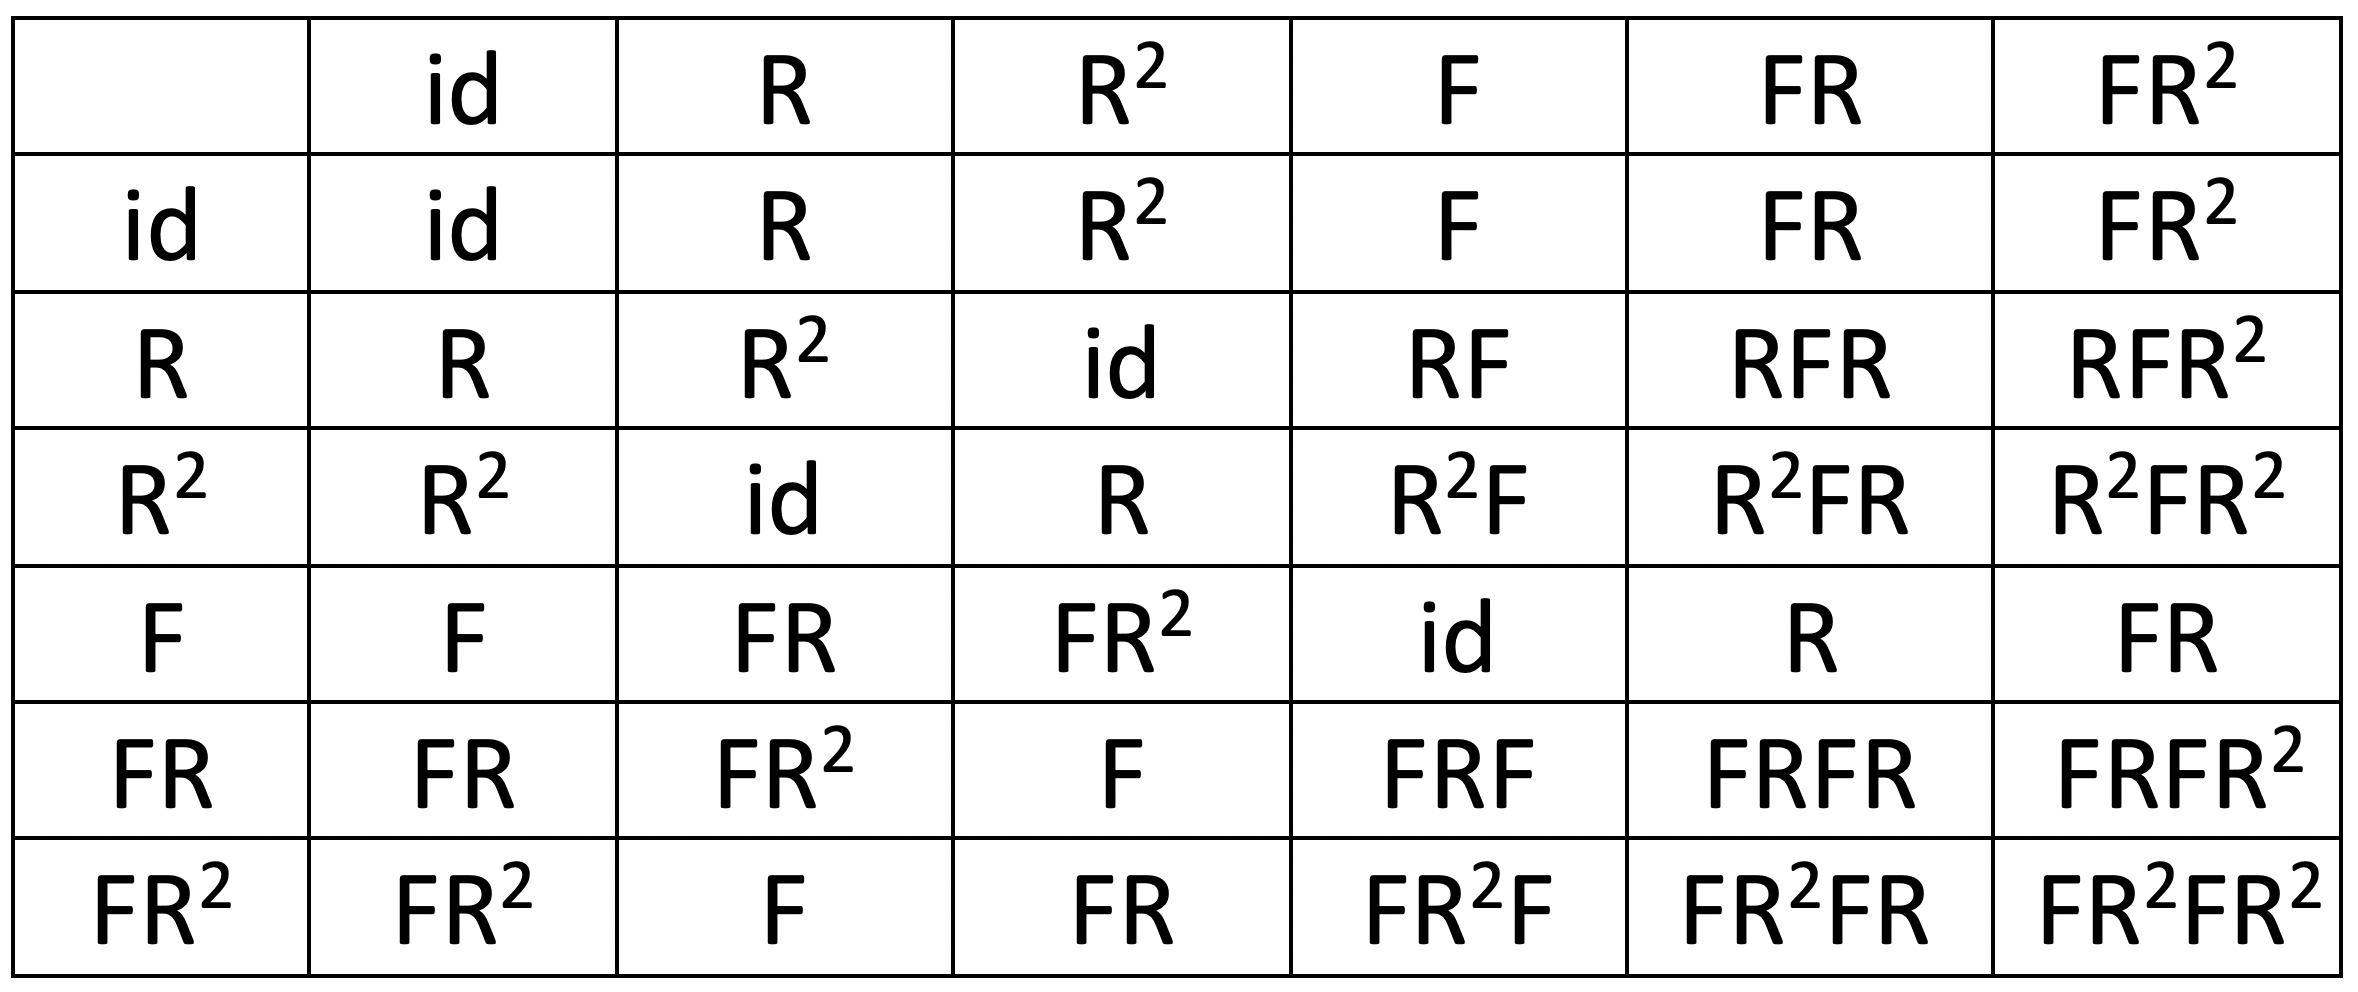
\includegraphics[width=0.48\linewidth]{figures/group_d3_m.png}
        }
%    \taco{TODO: figure of a triangle with labelled corners (0,1,2), and all permutations of it, as a Cayley diagram. Could add multiplication table of the group as well.}
    \caption{Left: an equilateral triangle with corners labelled by $1, 2, 3$, and all possible rotations and reflections of the triangle. The group $\mathrm{D}_3$ of rotation/reflection symmetries of the triangle is generated by only two elements (rotation by $60^\circ$ R and reflection F) and is the same as the group $\Sigma_3$ of permutations of three elements. 
    Right: the multiplication table of the group $\mathrm{D}_3$. The element in the row $\fg$ and column $\fh$ corresponds to the element $\fg \fh$. %\taco{\bf TODO: We need to reverse the Rotation arrows on the outer (or inner) ring. All rotations should be either clockwise or counter-clockwise}}
    \label{fig:group-example-d3-s3}
    }
\end{figure}

% Note that this definition provides a self-consistent description of a standalone object that is the main focus of study in group theory. Despite its apparent simplicity, this theory is rich with many deep results. 
% %despite the apparent simplicity of its basic definition.
% %
% %
% In geometry, key insights are obtained when transformations on a domain are modelled as elements of a group and the group theory formalism is used to study their properties --- this was exactly the breakthrough idea of Klein we have mentioned in the beginning of our discussion. 
% %
% %The way in which elements of symmetry groups act on points on a domain provides important insights about the structure of such domain --- 
% %
% %Group theory is a very rich area with many deep results, despite the apparent simplicity of its basic definition. 
% %
% %symmetry groups turn out to have rich internal algebraic structure with fascinating mathematical properties. 

\paragraph{Group Actions and Group Representations}
%
Rather than considering groups as abstract entities, 
we are mostly interested in how groups \emph{act} on data.
%The structure of such groups reveals the symmetry concealed in the data, which in turn leads to powerful geometric priors. 
%
%The assumption In geometric deep learning, one typically starts 
Since we assumed that there is some domain $\Omega$ underlying our data, we will study how the group acts on $\Omega$ 
(e.g. translation of points of the plane), and from there obtain actions of the same group on the space of signals $\mathcal{X}(\Omega)$
%\marginnote{Whenever possible, we will omit the range $\mathcal{C}$ for brevity.} %in which our data lives 
(e.g. translations of planar images and feature maps). 


% Taco: I am commenting this here, because 1) I think the notion of automorphism should be introduced differently. An auto is an iso from an object to itself. The meaning of iso depends on the context (category), i.e. on what properties/structure we wish to preserve. So when we introduce autos and subgroups, we should just say that we can preserve more or less structure, and get smaller or larger groups. 2) I think here the flow is disrupted a bit, and it would fit better in the deformation section.

% First, let us consider a broad class of bijective domain transformations called {\em automorphisms}
% $$\mathrm{Aut}(\Omega) = \{ \tau: \Omega \xrightarrow{1:1} \Omega \}.$$ 
% %
% Automorphisms also form a group with the composition operation. 
% %
% We can consider symmetries as `subsets' of automorphisms that preserve some structure: for example, in the plane the {\em Euclidean group} $\mathrm{E}(2)$ is the group of transformations of $\R^2$ that preserves Euclidean distances\marginnote{Distance-preserving transformations are called {\em isometries}. According to Klein's Erlangen Programme, the classical Euclidean geometry arises from this group.}, and consists of translations, rotations, and reflections.
% %
% More formally, a symmetry group $\fG$ constitutes a {\em subgroup} of the automorphism group $\mathrm{Aut}(\Omega)$: 

% \begin{tcolorbox}[width=\linewidth,
%                   boxsep=0pt,
%                   left=7.5pt,
%                   right=7.5pt,
%                   top=7.5pt,
%                   bottom=7.5pt,
%                   arc=0pt,
%                   boxrule=0pt,toprule=0pt,
%                   colback=boxgray,
%                   ]%%
% Let $(\fG,\circ)$ be a group and $\mathfrak{H} \subseteq \fG$ a subset. $\mathfrak{H}$ is said to be a {\em subgroup} of $\fG$ if $(\mathfrak{H},\circ)$ constitutes a group with the same operation. 
% \end{tcolorbox}


%we have considered so far are subgroups of $\mathrm{Aut}(\Omega)$. \marginnote{A subset $\fG \subseteq \frak{H}$ is said to be a {\em subgroup} of a group $(\frak{H}, \circ)$ if it forms a group $(\frak{G}, \circ)$ with the same operation.}



%\michael{do we use the . notation? $\fg.u$ of $\fg u$ but $\fg.x$}

A \emph{group action} \marginnote{Technically, what we define here is a {\em left} group action.} of $\fG$ on a set $\Omega$ 
%If $\fG$ is a group of transformations acting on elements of $\Omega$, a \emph{group action}\marginnote{Technically, what we define here is a {\em left} group action, since groups in general are non-commutative. } 
is defined as a mapping $(\fg, u) \mapsto \fg.u$ associating a group element $\fg \in \fG$ and a point $u\in \Omega$ with some other point on $\Omega$ in a way that 
%$(\fg, u) \mapsto \fg.u$
%$(g, x) \in \gG \times \gX \mapsto g.x \in \gX$, 
%that 
is compatible with the group operations, i.e., $\fg.(\fh.u) = (\fg \fh).u$ for all $\fg, \fh \in \fG$ and $u \in \Omega$. 
%
We shall see numerous instances of group actions in the following sections. 
%including translation groups acting on grids or permutation groups acting on sets and graphs.
% TODO: add definition block for group action?
%\michael{\bf [MB: is $g.x$ a standard notation? I suggest $\fg$ as notation for groups]}
%
%Most of the domains we will discuss in this book have some natural symmetries. 
For example, in the plane the {\em Euclidean group} $\mathrm{E}(2)$ is the group of transformations of $\R^2$ that preserves Euclidean distances\marginnote{Distance-preserving transformations are called {\em isometries}. According to Klein's Erlangen Programme, the classical Euclidean geometry arises from this group.}, and consists of translations, rotations, and reflections.
%collection of translation, rotation, and reflection transformations preserving Euclidean distances, so this group acts naturally on the plane.
The same group, however, can also act on the space of \emph{images} on the plane (by translating, rotating and flipping the grid of pixels), as well as on the representation spaces learned by a neural network.
%
%
More precisely, if we have a group $\fG$ acting on $\Omega$, we automatically obtain an action of $\fG$ on the space $\mathcal{X}(\Omega)$: 
%\marginnote{When it is clear from the context, we shall simplify the notation and simply write $\mathcal{X}$ for such space.}
%\michael{Do we need to carry the C here? It is not used; we only need to say that X is a vector space. I suggest to simplify the notation as much as possible. }
\begin{equation}
    (\fg . x)(u) = x(\fg^{-1} u).
    \label{eq:group_action}
\end{equation}
Due to the inverse on $\fg$, this is indeed a valid group action, in that we have $(\fg . (\fh . x))(u) = ((\fg \fh) . x)(u)$.  %(exercise).
%: $(\fg . (\fh . f))(x) = (\fh . f)(\fg^{-1} x) = f(\fh^{-1} \fg^{-1} x) = f((\fg \fh)^{-1} x) = ((\fg \fh). f)(x)$. % leave as exercise?
%\michael{Is this standard notation? Looks abusive to use . for action on $x$ and $u$.}

%
%In our context, the central importance of symmetry groups is due to the fact that they also interact nicely with other less-structured objects. If $\fG$ is a group of transformations acting on elements of some arbitrary set $\gX$, a \emph{group action} is defined as a mapping 
%$(\fg, x) \mapsto \fg.x$
%$(g, x) \in \gG \times \gX \mapsto g.x \in \gX$, 
%that is compatible with the group operations in the sense that $\fg.(\fh.x) = (\fg \circ \fh).x$ for all $\fg, \fh \in \fG$ and $x \in \gX$. We shall see numerous instances of group actions in the next chapters, including translation groups acting on grids or permutation groups acting on sets and graphs.
% TODO: add definition block for group action?
%\michael{\bf [MB: is $g.x$ a standard notation? I suggest $\fg$ as notation for groups]}

The most important kind of group actions, which we will encounter repeatedly throughout this text, are \emph{linear} group actions, also known as {\em group representations}.
The action on signals in equation~(\ref{eq:group_action}) is indeed linear, in the sense that 
$$
\fg . (\alpha x + \beta x') = \alpha (\fg . x) + \beta (\fg . x') $$
%
for any scalars $\alpha, \beta$ and signals $x, x' \in \mathcal{X}(\Omega)$. 
%
We can describe linear actions either as maps $(\fg, x) \mapsto \fg.x$ that are linear in $x$, or equivalently, by currying, 
%\footnote{Currying is the technique of converting a function that takes multiple arguments into a sequence of functions that each take a single argument.}
as a map $\rho : \fG \rightarrow \R^{n \times n}$\marginnote{When $\Omega$ is infinte, the space of signals $\mathcal{X}(\Omega)$ is infinite dimensional, in which case $\rho(\fg)$ is a linear operator on this space, rather than a finite dimensional matrix. In practice, one must always discretise to a finite grid, though.} that assigns to each group element $\fg$ an (invertible) matrix $\rho(\fg)$.
%\michael{Do we want to say representation can be over different space, and here we are interested in the space of signals? We need to say this is a vector space. }
The dimension $n$ of the matrix is in general arbitrary and not necessarily related to the dimensionality of the group or the dimensionality of $\Omega$, but in applications to deep learning $n$ will usually be the dimensionality of the feature space on which the group acts.
For instance, we may have the group of 2D translations acting on a space of images with $n$ pixels.

%\michael{\bf [MB: $n$ has to be defined. This paragraph needs a bit more details/polishing]}
As with a general group action, the assignment of matrices to group elements should be compatible with the group action.
More specifically, the matrix representing a composite group element $\fg \fh$ should equal the matrix product of the representation of $\fg$ and $\fh$:
%\begin{equation}
%    \rho(\fg \fh) = \rho(\fg) \rho(\fh).
%\end{equation}
%\michael{Can we just call this associativity? } \taco{No; both the group operation $\fg \fh$ and the matrix product $\rho(\fg) \rho(\fh)$ are associative, but the equation here says that $\rho$ is a homomorphism. Associativity involves three things being multiplied, $a(bc) = (ab)c$, but here we have two group elements $\fg, \fh$ and one mapping $\rho$, so it's different.}

% History of symmetries in mathematics and physics:
% \begin{itemize}
%     \item Kepler laws of planetary motion. 
%     \item Lagrangian and Hamiltonian of Mechanics invariant to observer frame of reference. 
%     \item Relativity? 
%     \item In mathematics, example of Galois Theory to study the roots of polynomial equations. The structure of such roots is revealed by studying their symmetries. 
% \end{itemize}

\begin{tcolorbox}[width=\linewidth,
                  boxsep=0pt,
                  left=7.5pt,
                  right=7.5pt,
                  top=7.5pt,
                  bottom=7.5pt,
                  arc=0pt,
                  boxrule=0pt,toprule=0pt,
                  colback=boxgray,
                  ]%%
    A $n$-dimensional real \emph{representation} of a group $\fG$ is a map $\rho : \fG \rightarrow \R^{n \times n}$, assigning to each $\fg \in \fG$ an \emph{invertible} matrix $\rho(\fg)$, and satisfying the condition $\rho(\fg \fh) = \rho(\fg) \rho(\fh)$ for all $\fg, \fh \in \fG$.
    \marginnote{Similarly, a complex representation is a map $\rho : \fG \rightarrow \mathbb{C}^{n \times n}$ satisfying the same equation.}
    A representation is called \emph{unitary} or \emph{orthogonal} if the matrix $\rho(\fg)$ is unitary or orthogonal for all $\fg \in \fG$.
\end{tcolorbox}

Written in the language of group representations, the action of $\fG$ on signals $x \in \mathcal{X}(\Omega)$ is defined as $\rho(\fg) x(u) = x(\fg^{-1} u)$.
%
We again verify that 
$$
(\rho(\fg) (\rho(\fh) x))(u) = (\rho(\fg \fh) x)(u).
$$
%



% Removing stuff on subgroups and homogeneous spaces, as we don't really need it to talk about groups, representations and equivariance.
% % Consider moving this right after the definition of group, since the notion of subgroup does not rely on the notion of group action... 
% A subset of a group that is itself a group (i.e. is closed under composition and inverses, and contains the identity) is called a \emph{subgroup}.
% For example, the group $\mathrm{E}(2)$ contains the subset of rotations and translations (also called `roto-translations'), which is closed under composition and forms a group called the {\em special Euclidean group} $\SE{2}$. Finally, translations by themselves form the {\em translation group}. 
% %


% The plane is an example of a space in which ``all points are the same'', in the sense that one point can be transformed into another by means of a symmetry. 
% %
% Such a space is said to be {\em homogeneous} and requires that for any two points $u, v \in \Omega$ there is $\fg \in \fG$ such that $u = \fg v$. 
% %or in other words, one point can be transformed into another by means of a symmetry. 


\begin{figure}
    \centering
    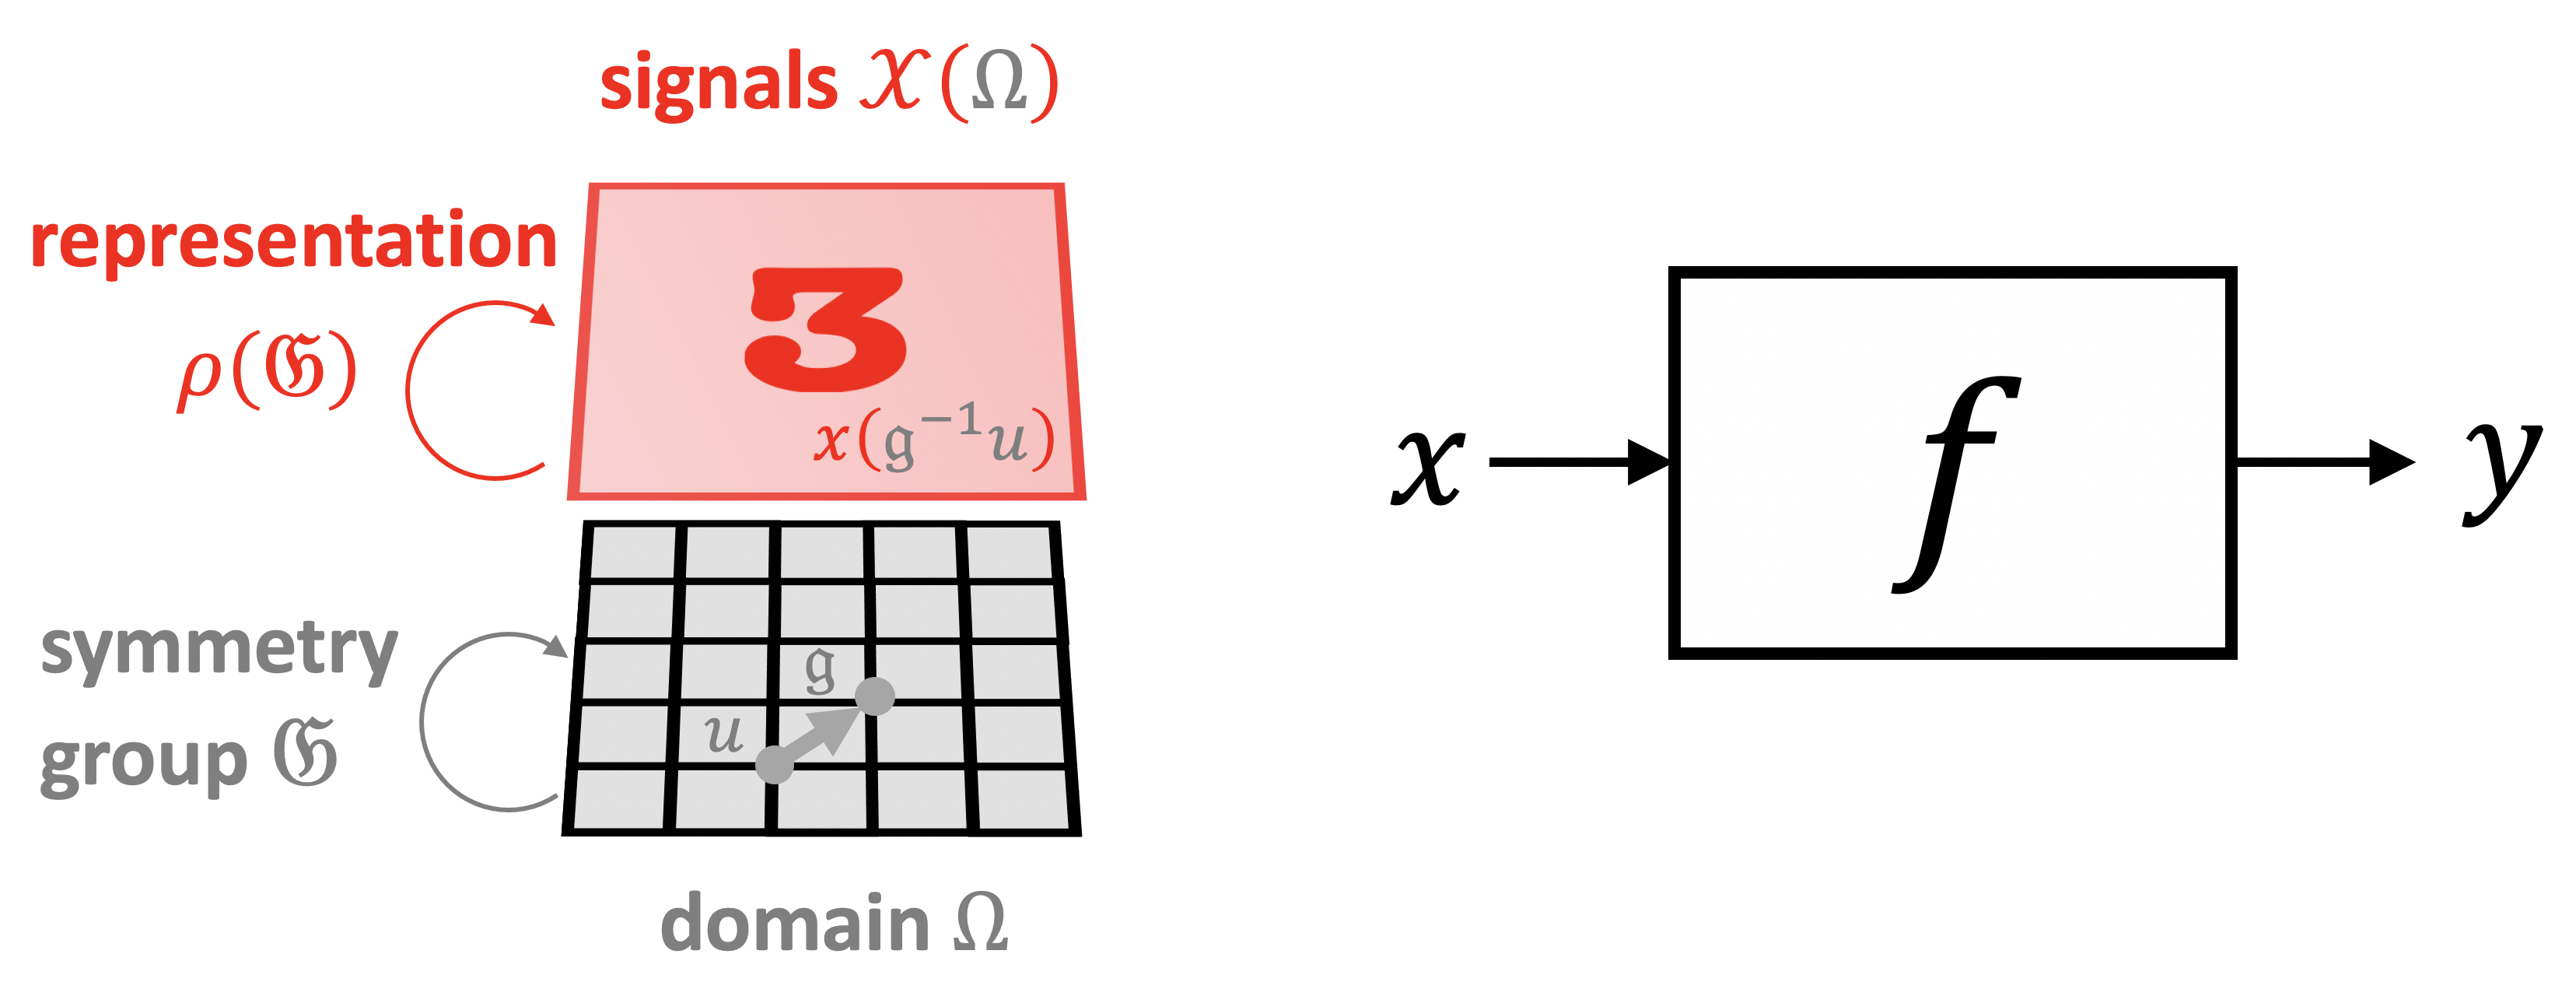
\includegraphics[width=0.75\linewidth]{figures/geom_prior.png}%groups1.pdf}
    \caption{
    Three spaces of interest in Geometric Deep Learning: the (physical) {\em domain} $\Omega$, the space of {\em signals} $\mathcal{X}(\Omega)$, and the {\em hypothesis} class $\mathcal{F}(\mathcal{X}(\Omega))$. 
    %
    Symmetries of the domain $\Omega$ (captured by the group $\fG$) act on signals $x\in \mathcal{X}(\Omega)$ through group representations $\rho(\fg)$, imposing structure on the functions $f\in \mathcal{F}(\mathcal{X}(\Omega))$ acting on such signals.
    }
    \label{fig:symmetryactors}
\end{figure}


\paragraph{Invariant and Equivariant functions}

The symmetry of the domain $\Omega$ underlying the signals $\mathcal{X}(\Omega)$ imposes structure on the function $f$ defined on such signals. 
%
It turns out to be a powerful inductive bias, improving learning\marginnote{In general, $f$ depends both on the signal an the domain, i.e., $\mathcal{F}(\mathcal{X}(\Omega), \Omega)$. We will often omit the latter dependency for brevity. } efficiency by reducing the space of possible interpolants, $\mathcal{F}(\mathcal{X}(\Omega))$, to those which satisfy the symmetry priors. 
%
%Adding such known symmetries into the function hypothesis class of a machine learning system is a powerful inductive bias, improving learning efficiency by reducing the space of possible interpolants to those which satisfy the symmetry priors. 
%
Two important cases we will be exploring in this text are {\em invariant} and {\em equivariant} functions. 


%is its output is unaffected by the action of the group on the argument


\begin{tcolorbox}[width=\linewidth,
                  boxsep=0pt,
                  left=7.5pt,
                  right=7.5pt,
                  top=7.5pt,
                  bottom=7.5pt,
                  arc=0pt,
                  boxrule=0pt,toprule=0pt,
                  colback=boxgray,
                  ]%%
    A function $f: \mathcal{X}(\Omega) \rightarrow \mathcal{Y}$ is $\fG$-{\em invariant} if 
    $
    f(\rho(\fg)x) = f(x)$  for all $\fg \in \fG$ and $x \in \mathcal{X}(\Omega)$, i.e., its output is unaffected by the group action on the input. 
\end{tcolorbox}


A classical example of invariance is {\em shift-invariance},\marginnote{Note that signal processing books routinely use the term `shift-invariance' referring to shift-equivariance, e.g. Linear Shift-invariant Systems. } 
arising in computer vision and pattern recognition applications such as image classification. The function $f$ in this case (typically implemented as a Convolutional Neural Network) inputs an image and outputs the probability of the image to contain an object from a certain class (e.g. cat or dog). %
%
It is often reasonably assumed that the classification result should not be affected by the position of the object in the image, i.e., the function $f$ must be shift-invariant. 
%
Multi-layer Perceptrons, which can approximate any smooth function, do not have this property -- one of the reasons why early attempts to apply these architectures to problems of pattern recognition in the 1970s failed. 
%
The development of neural network architectures with local weight sharing, as epitomised by Convolutional Neural Networks, was, among other reasons, motivated by the need for shift-invariant object classification. 


If we however take a closer look at the convolutional layers of CNNs, we will find that they are not shift-invariant but {\em shift-equivariant}: in other words, a shift of the input to a convolutional layer produces a shift in the output feature maps by the same amount. 

\begin{tcolorbox}[width=\linewidth,
                  boxsep=0pt,
                  left=7.5pt,
                  right=7.5pt,
                  top=7.5pt,
                  bottom=7.5pt,
                  arc=0pt,
                  boxrule=0pt,toprule=0pt,
                  colback=boxgray,
                  ]%%
    A function $f: \mathcal{X}(\Omega) \rightarrow \mathcal{X}(\Omega)$ is $\fG$-{\em equivariant} if\marginnote{
    More generally, we might have $f: \mathcal{X}(\Omega) \rightarrow \mathcal{X}(\Omega')$ with input and output spaces having different domains $\Omega, \Omega'$ and representations $\rho$, $\rho'$ of the same group $\fG$.
    In this case, equivariance is defined as $f(\rho(\fg)x) = \rho'(\fg) f(x)$.
    %symmetry groups, $\fG$ and $\fG'$. In this case, equivariance is defined as $ f(\rho(\fg)x) = \rho'(\fg) f(x)$, where $\rho'$ is the representation of $\fG'$.
    } 
    $f(\rho(\fg)x) = \rho(\fg) f(x)$  for all $\fg \in \fG$, i.e., group action on the input affects the output in the same way. 
\end{tcolorbox}




Resorting again to computer vision, a prototypical application requiring shift-equivariance is image segmentation, where the output of $f$ is a pixel-wise image mask. 
%
Obviously, the segmentation mask must follow shifts in the input image.  
In this example, the domains of the input and output are the same, but since the input has three color channels while the output has one channel per class, the representations $(\rho, \mathcal{X}(\Omega, \mathcal{C}))$ and $(\rho', \mathcal{X}(\Omega, \mathcal{C}'))$ are somewhat different.


However, even the previous use case of image classification is usually implemented as a sequence of convolutional (shift-equivariant) layers, followed by global pooling (which is shift-invariant). 
%
As we will see in Section~\ref{sec:gdl_blueprint}, this is a general blueprint of a majority of deep learning architectures, including CNNs and Graph Neural Networks (GNNs). 
%: a sequence of equivariant layers, optionally followed by invariant layers. 


%In supervised learning, the goal is to approximate some function $f : \mathcal{X} \rightarrow \mathcal{X}'$ from a finite set of samples.
%In many cases, the problem has symmetries, which means that $f$ is either invariant ($f(\rho(\fg) x) = f(x)$ for all $\fg \in \fG$) or equivariant ($f(\rho(\fg) x) = \rho'(\fg) f(x)$).
%For instance, in image classification the class label is invariant, whereas the segmentation mask is equivariant. 
% In machine learning, where one tries to approximate some unknown function $f$ from a finite set of samples, $f$ often has known symmetries.
% Canonical examples include translations in computer vision and image classification tasks, rotations in molecular prediction problems, or permutations in 3D graphics point-cloud processing tasks. 
% %
% In such settings, given some domain $\gX$ with a certain symmetry group $\fG$, we say that 
% $f: \gX \to \gY$ is $\fG$\emph{-invariant} if $f(\fg.x) = f(x)$ for all $x\in \gX$ and $\fg \in \fG$. If in addition $\fG$ is also acting on $\gY$, we say that $f$ is $\fG$\emph{-equivariant} if $f(\fg.x) = \fg.(f(x))$.
% % We will explore these concepts in detail in Chapter ??. 
%Adding such known symmetries into the function hypothesis class %$\gF$ 
%of a machine learning system is a powerful inductive bias, improving learning efficiency by reducing the space of possible interpolants to those which satisfy the symmetry priors. 


% Possible todo's for this section:
% Explain in/equivariance mathematically (at a high level only)
% Explain group representations (idem)


%\taco{TODO: add definition of space of signals, and regular rep acting on it}

%\taco{TODO: Figure showing domain Omega, group action of G on Omega, and the space of functions X on Omega}

\subsection{Isomorphisms and Automorphisms}
\label{sec:isomorphism}

\paragraph{Subgroups and Levels of structure}

As mentioned before, a symmetry\marginnote{Invertible and structure-preserving maps between different objects often go under the generic name of {\em isomorphisms} (Greek for `equal shape'). An isomorphism from an object to itself is called an {\em automorphism}, or symmetry.}
%We will mainly use this term for maps preserving the connectivity of graphs.}
is a transformation that preserves some property or structure, and the set of all such transformations for a given structure forms a symmetry group.
It happens often that there is not one but multiple structures of interest, and so we can consider several {\em levels of structure} on our domain $\Omega$. 
%
%We can thus formalise symmetries as invertible maps $\tau: \Omega \rightarrow \Omega$ that preserve some structure. % and satisfy the group axioms with the function composition operation.  
Hence, what counts as a symmetry depends on the structure under consideration, but in all cases a symmetry is an invertible map that respects this structure.

On the most basic level, the domain $\Omega$ is a \emph{set}, which has a minimal amount of structure: all we can say is that the set has some \emph{cardinality}\marginnote{For a finite set, the cardinality is the number of elements (`size') of the set, and for infinite sets the cardinality indicates different kinds of infinities, such as the countable infinity of the natural numbers, or the uncountable infinity of the continuum $\R$.}. %, and which elements are members of the set.
Self-maps that preserve this structure are  \emph{bijections} (invertible maps), which we may consider as set-level symmetries.
%A more formal way to say the same is that the automorphism group $\mathrm{Aut}(\Omega)$ in the category of sets is the group of bijections $\tau : \Omega \rightarrow \Omega$.
%Such maps are often referred to as (set-){\em automorphisms} and denoted by $\mathrm{Aut}(\Omega)$. 
%
One can easily verify that this is a group by checking the axioms: a compositions of two bijections is also a bijection (closure), the associativity stems from the associativity of the function composition, the map $\tau(u)=u$ is the identity element, and for every $\tau$ the inverse exists by definition, satisfying $(\tau \circ \tau^{-1})(u) = (\tau^{-1} \circ \tau)(u) =u$.


Depending on the application, there may be further levels of structure.  
%
For instance, if $\Omega$ is a topological space, we can consider maps that preserve {\em continuity}: such maps are called {\em homeomorphisms} and in addition to simple bijections between sets, are also continuous and have continuous inverse.  
%
Intuitively, continuous functions are well-behaved and map points in a neighbourhood (open set) around a point $u$ to a neighbourhood around $\tau(u)$.  
%Thus, homeomorphisms $\tau : \Omega \rightarrow \Omega$ are the automorphisms / symmetries of $\Omega$ viewed as a topological space.


%
%
One can further demand that the map and its inverse are (continuously) {\em  differentiable},\marginnote{Every differentiable function is continuous. If the map is continuously differentiable `sufficiently many times', it is said to be {\em smooth}.} i.e., the map and its inverse have a derivative at every point (and the derivative is also continuous). 
%
This requires further differentiable structure that comes with differentiable manifolds, where such maps are called {\em diffeomorphisms} and denoted by $\mathrm{Diff}(\Omega)$. 
%These are the automorphisms of smooth manifolds.
%
%
Additional examples of structures we will encounter include {\em distances} or {\em metrics} (maps preserving them are called {\em isometries}) or {\em orientation} (to the best of our knowledge, orientation-preserving maps do not have a common Greek name). 


\begin{tcolorbox}[width=\linewidth,
                  boxsep=0pt,
                  left=7.5pt,
                  right=7.5pt,
                  top=7.5pt,
                  bottom=7.5pt,
                  arc=0pt,
                  boxrule=0pt,toprule=0pt,
                  colback=boxgray,
                  ]%%
A {\em metric} or {\em distance} is a function $d:\Omega\times\Omega \rightarrow [0,\infty)$ satisfying for all $u,v,w \in \Omega$:  \vspace{3mm}\\
%\begin{enumerate}
    %\item 
    \noindent {\em 	Identity of indiscernibles:} $d(u,v) =0$ iff $u=v$.\vspace{2mm}\\
    \noindent  {\em Symmetry:} $d(u,v) = d(v,u)$.\vspace{2mm}\\
    \noindent  {\em Triangle inequality:} $d(u,v) \leq  d(u,w) + d(w,v)$.\vspace{2mm}\\
%\end{enumerate}

A space equipped with a metric $(\Omega,d)$ is called a {\em metric space}. 

\end{tcolorbox}




%an image plane can be viewed as a smooth manifold, in which case any smooth deformation (diffeomorphism) should be considered a symmetry.
%In practice the object identity will not be preserved by arbitrarily large deformations, so we may add a distance metric, i.e. view the image plane as a Riemannian manifold, in which case only distance-preserving transformations (isometries) can be considered as symmetries.
%As a further example, independently of whether we care about distances, we can assign an \emph{orientation} to the plane, i.e. clockwise or counterclockwise, and consider only orientation-preserving transformations.

The right level of structure to consider depends on the problem.
For example, when segmenting histopathology slide images, we may wish to consider flipped versions of an image as equivalent (as the sample can be flipped when put under the microscope), but if we are trying to classify road signs, we would only want to consider orientation-preserving transformations as symmetries (since reflections could change the meaning of the sign).
%{\bf [Figure?]}

As we add levels of structure to be preserved, the symmetry group will get smaller.
Indeed, adding structure is equivalent to selecting a \emph{subgroup}, which is a subset of the larger group that satisfies the axioms of a group by itself:  
%(i.e. it is closed under composition and inverses, and contains the identity).
 
 \begin{tcolorbox}[width=\linewidth,
                   boxsep=0pt,
                   left=7.5pt,
                   right=7.5pt,
                   top=7.5pt,
                   bottom=7.5pt,
                   arc=0pt,
                   boxrule=0pt,toprule=0pt,
                   colback=boxgray,
                   ]%%
 Let $(\fG,\circ)$ be a group and $\mathfrak{H} \subseteq \fG$ a subset. $\mathfrak{H}$ is said to be a {\em subgroup} of $\fG$ if $(\mathfrak{H},\circ)$ constitutes a group with the same operation. 
 \end{tcolorbox}
 
For instance, the group of Euclidean isometries $\E{2}$ is a subgroup of the group of planar diffeomorphisms $\diff{2}$, and in turn the group of orientation-preserving isometries $\SE{2}$ is a subgroup of $\E{2}$.
This hierarchy of structure follows the Erlangen Programme philosophy outlined in the Preface: in Klein's construction, the Projective, Affine, and Euclidean geometries have increasingly more invariants and correspond to progressively smaller groups. 


\paragraph{Isomorphisms and Automorphisms}
% Optional: discuss the notion of isomorphic objects, and present symmetries as self-isomorphisms i.e. automorphisms. Thus the notion of symmetry depends on the notion of iso, i.e. the category we're working in, i.e. the level of structure as discussed above.

We have described symmetries as structure preserving and invertible maps \emph{from an object to itself}.
Such maps are also known as \emph{automorphisms}, and describe a way in which an object is equivalent it itself.
However, an equally important class of maps are the so-called \emph{isomorphisms}, which exhibit an equivalence between two non-identical objects.
These concepts are often conflated, but distinguishing them is necessary to create  clarity for our following discussion.

To understand the difference, consider a set $\Omega = \{0,1,2\}$.
An automorphism of the set $\Omega$ is a bijection $\tau : \Omega \rightarrow \Omega$ such as a cyclic shift $\tau(u) = u + 1 \mod 3$.
Such a map preserves the cardinality property, and maps $\Omega$ onto itself.
If we have another set $\Omega' = \{a, b, c\}$ with the same number of elements, then a bijection $\eta : \Omega \rightarrow \Omega'$ such as $\eta(0) = a$, $\eta(1) = b$, $\eta(2) = c$ is a {\em set isomorphism}.

As we will see in Section~\ref{sec:proto-graphs}
for graphs, %$\Omega$, 
the notion of structure includes not just the number of nodes, but also the connectivity.
An isomorphism $\eta: \mathcal{V} \rightarrow \mathcal{V}'$ between two graphs $\mathcal{G}=(\mathcal{V},\mathcal{E})$ and $\mathcal{G}'=(\mathcal{V}',\mathcal{E}')$ is thus a bijection between the nodes that maps pairs of connected nodes to pairs of connected nodes, and likewise for pairs of non-connected nodes.\marginnote{I.e., $(\eta(u),\eta(v)) \in \mathcal{V}'$ iff $(u,v) \in \mathcal{V}$. } Two isomorphic graphs are thus structurally identical, and differ only in the way their nodes are ordered. \marginnote{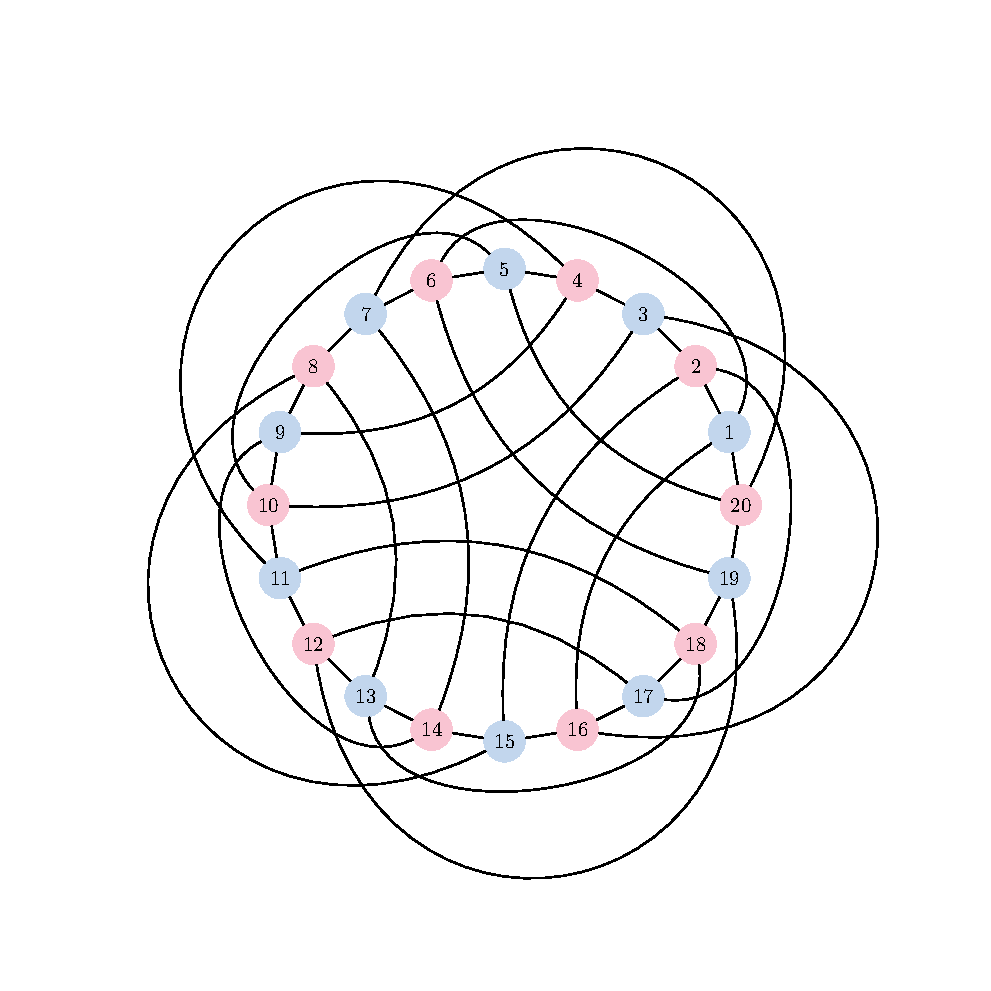
\includegraphics[width=\linewidth]{figures/folkman_g.pdf}\vspace{-2mm}\\ The \emph{Folkman graph} \citep{folkman1967regular} is a beautiful example of a graph with 3840  automorphisms, exemplified by the many symmetric ways to draw it.}
%
On the other hand, a graph automorphism or symmetry is a map $\tau : \mathcal{V} \rightarrow \mathcal{V}$ maps the nodes of the graph back to itself, while preserving the connectivity. A graph with a non-trivial automorphism (i.e., $\tau \neq \mathrm{id}$) presents symmetries.
%\michael{Show in a figure}

%An isomorphism of graphs is thus not the same as a symmetry, but it is just as important that our neural network treat isomorphic objects equivalently.
% when we're dealing with isos vs autos. Example of sphere and graph

% same number of isos A -> B and autos A -> A. Isomorphic objects have isomorphic automorphism groups




\subsection{Deformation Stability}
\label{sec:geom_stab}
%While the Fourier representation is useful to represent {\em signals} $\gX(\Omega)$ on a domain $\Omega$, it is not necessarily useful to regularise the space of {\em functions on such signals}, $\mathcal{F}(\mathcal{X}(\Omega))$ used in supervised learning problems. 
%
%Despite its far-reaching implications, the Fourier representation $\hat{x}$ is not necessarily useful to regularise the space of functions $\{ f : \gX \to \gY \}$, 
%the ultimate goal of supervised learning. 
%
The symmetry formalism introduced in Sections~\ref{sec:symmetries}--\ref{sec:isomorphism} captures an idealised world where we know exactly which transformations are to be considered as symmetries, and we want to respect these symmetries {\em exactly}. 
%the transformations affecting the input are captured with simple mathematical models.
For instance in computer vision, we might assume that planar translations are exact symmetries.
%model for input variability parametrised by only two degrees of freedom (the translations in the plane). 
However, the real world is noisy and this model falls short in two ways. %: it only describes \emph{global} transformations, and 

\marginnote{
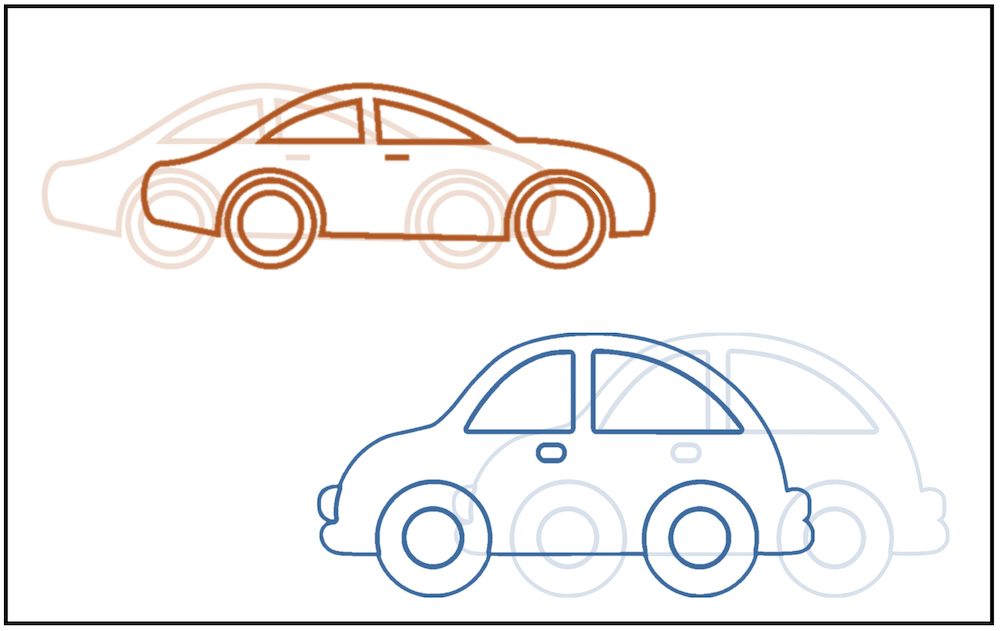
\includegraphics[width=0.95\linewidth]{figures/videosketch.png}
Two objects moving at different velocities in a video define 
a transformation outside the translation group.
}
Firstly, while these simple groups provide a way to understand \emph{global} symmetries of the domain $\Omega$ (and by extension, of signals on it, $\gX(\Omega)$), they do not capture \emph{local} symmetries well. 
%
For instance, consider a video scene %$x=x_t$ 
with several objects, each moving along its own different direction.
At subsequent frames, the resulting scene 
%$x_{t+\delta t}$ 
will contain approximately the same semantic information, yet no global translation explains the transformation from one frame to another.
In other cases, such as a deformable 3D object viewed by a camera, it is simply very hard to describe the group of transformations that preserve the object identity.
These examples illustrate that in reality we are more interested in a %beneath the global symmetry group lies a 
far larger set of transformations where global, exact invariance is replaced by a local, inexact one.
%
In our discussion, we will distinguish between two scenarios: the setting where the domain $\Omega$ is fixed, and signals $x \in \gX(\Omega)$ are undergoing deformations, and the setting where the domain $\Omega$ itself may be deformed.
%\taco{TODO: perhaps move this up, and discuss this as isomorphisms vs automorphisms?}

%In the language of group representations, we thus need to account for a broader class of bijective domain transformations called {\em automorphisms}, $\mathrm{Aut}(\Omega) = \{ \tau: \Omega \xrightarrow{1:1} \Omega \}$. 
\paragraph{Stability to signal deformations}
In many applications, we know a priori that a small deformation of the signal $x$ should not change the output of $f(x)$, so it is tempting to consider such deformations as symmetries.
For instance, we could view small diffeomorphisms $\tau \in \diff{\Omega}$, or even small bijections, as symmetries.
However, small deformations can be composed to form large deformations, so ``small deformations'' do not form a group,\marginnote{E.g., the composition of two $\epsilon$-isometries is a $2\epsilon$-isometry, violating the closure property. } and we cannot ask for invariance or equivariance to small deformations only.
Since large deformations can can actually materially change the semantic content of the input, it is not a good idea to use the full group $\diff{\Omega}$ as symmetry group either.

A better approach is to quantify how ``far'' a given $\tau \in \diff{\Omega}$ is from a given symmetry subgroup $\fG \subset \diff{\Omega}$ (e.g. translations)
with a complexity measure $c(\tau)$, so that $c(\tau) = 0$ whenever $\tau \in \fG$. 
We can now replace our previous  definition of exact invariance and equivarance under group actions with a `softer' notion of  
\emph{deformation stability} (or {\em approximate invariance}):
\begin{equation}
\label{eq:defstability1}
\| f(\rho(\tau) x) - f(x)\| \leq C c(\tau) \|x\|,~,~    \forall x\in \gX(\Omega)
\end{equation}
where $\rho(\tau)x(u) = x(\tau^{-1} u)$ as before, and where $C$ is some constant independent of the signal $x$. 
A function $f\in \mathcal{F}(\mathcal{X}(\Omega))$ satisfying the above equation is said to be {\em geometrically stable}. 
%
We will see examples of such functions in the next Section~\ref{sec:scale_separation}. 


Since $c(\tau)=0$ for $\tau \in \fG$, this definition generalises the $\fG$-invariance property defined above. Its utility in applications depends on introducing an appropriate deformation cost. In the case of images defined over a continuous Euclidean plane, 
a popular choice is $c^2(\tau) := \int_\Omega \| \nabla \tau(u)\|^2 \mathrm{d}u$, which measures the `elasticity' of $\tau$, i.e., how different it is from the displacement by a constant vector field. 
%
This deformation cost is in fact a norm often called the {\em Dirichlet energy}, and can be used to quantify how far $\tau$ is from the translation group. 

%


% All of the symmetry groups we have considered and will consider in this book are subgroups of the group of bijections of $\Omega$.
% %The symmetry groups we have considered so far are subgroups of the group $\mathrm{Aut}(\Omega)$ of set-automorphisms of $\Omega$, or general domain transformations. 
% %
% For any such group $\fG$, 

% Same way as we had the symmetry group $\fG$ represented as a linear operator $\rho$ on $\mathcal{X}(\Omega)$, we can now do the same for $\mathrm{Aut}(\Omega)$ to lift diffeomorphisms of the domain into linear transformations on signals $x \in \gX(\Omega)$:
% %construct a linear operator $L_\tau: \gX(\Omega) \to \gX(\Omega)$ of the form 
% %that extend group actions, and which again lift into linear transformations , 
% $$
% (\rho(\tau) x)(u) = x( \tau^{-1}(u)). 
% $$  
% %$\rho(\fg), \fg \in \fG$, we thus need to consider linear transformations
% %
% This represents how the transformation of the domain $\Omega$ by an automorphism $\tau$ affects the signal $x \in \mathcal{X}(\Omega)$; see Figure \ref{fig:groupdeformation}. %
% Note that invariance to such large automorphism group is not a desired property, since large distortions of the domain 
% eventually destroy the semantic information of the input. 
% Instead, we can quantify how "far" a given $\tau \in \mathrm{Aut}(\Omega)$ is from a given symmetry subgroup $\fG \subset \mathrm{Aut}(\Omega)$ 
% with a complexity measure $c(\tau)$, so that $c(\tau) = 0$ whenever $\tau \in \fG$. 
% We can now replace our previous rigid definition of invariance and equivarance under group actions to a softer 
% \emph{deformation stability} principle:
% %Similarly to our definition of functions that are invariant and equivariant under group actions, 
% %we can have functions that are {\em approximately invariant} or {\em equivariant} under such automorphisms. 
% %
% %Such approximate invariance, to which we refer as {\em geometric stability}, can be expressed in the form of a bound %of the form
% \begin{equation}
% \label{eq:defstability1}
% \forall ~x\in \gX(\Omega)~,~\| f(\rho(\tau) x) - f(x)\| \leq C c(\tau) \|x\|,    
% \end{equation}
% with some constant $C$ independent of the signal $x$. A function $f\in \mathcal{F}(\mathcal{X}(\Omega))$ satisfying the above equation is said to be {\em geometrically stable}. 
% %
% Since $c(\tau)=0$ for $\tau \in \fG$, this definition generalises the $\fG$-invariance property defined above. Its utility in applications depends on introducing an appropriate deformation cost. In the case of images defined over a continuous Euclidean plane, 
% a relevant example is given by $c^2(\tau) := \int_\Omega \| \nabla \tau(u)\|^2 \mathrm{d}u$. This deformation cost is in fact a norm often called the {\em Dirichlet energy}, and used as a measure of elasticity of $\tau$. 
% %We will discuss these concepts in greater detail in Chapter ???.

% %To quantify this properly, we need some notion of metric or `distance' between maps and signals, as will be detailed in Section ??.  
% %
% %In some sense that will be formalized later, we expect our functions of interest to be \emph{almost} invariant/equivariant for transformations $L_\tau$ which are ``nearby" the group transformations $\rho(\fg)$ for $\fg \in \fG$.
% %We informally refer to this concept as \emph{geometric stability}. 

\begin{figure}[!htbp]
    \centering
    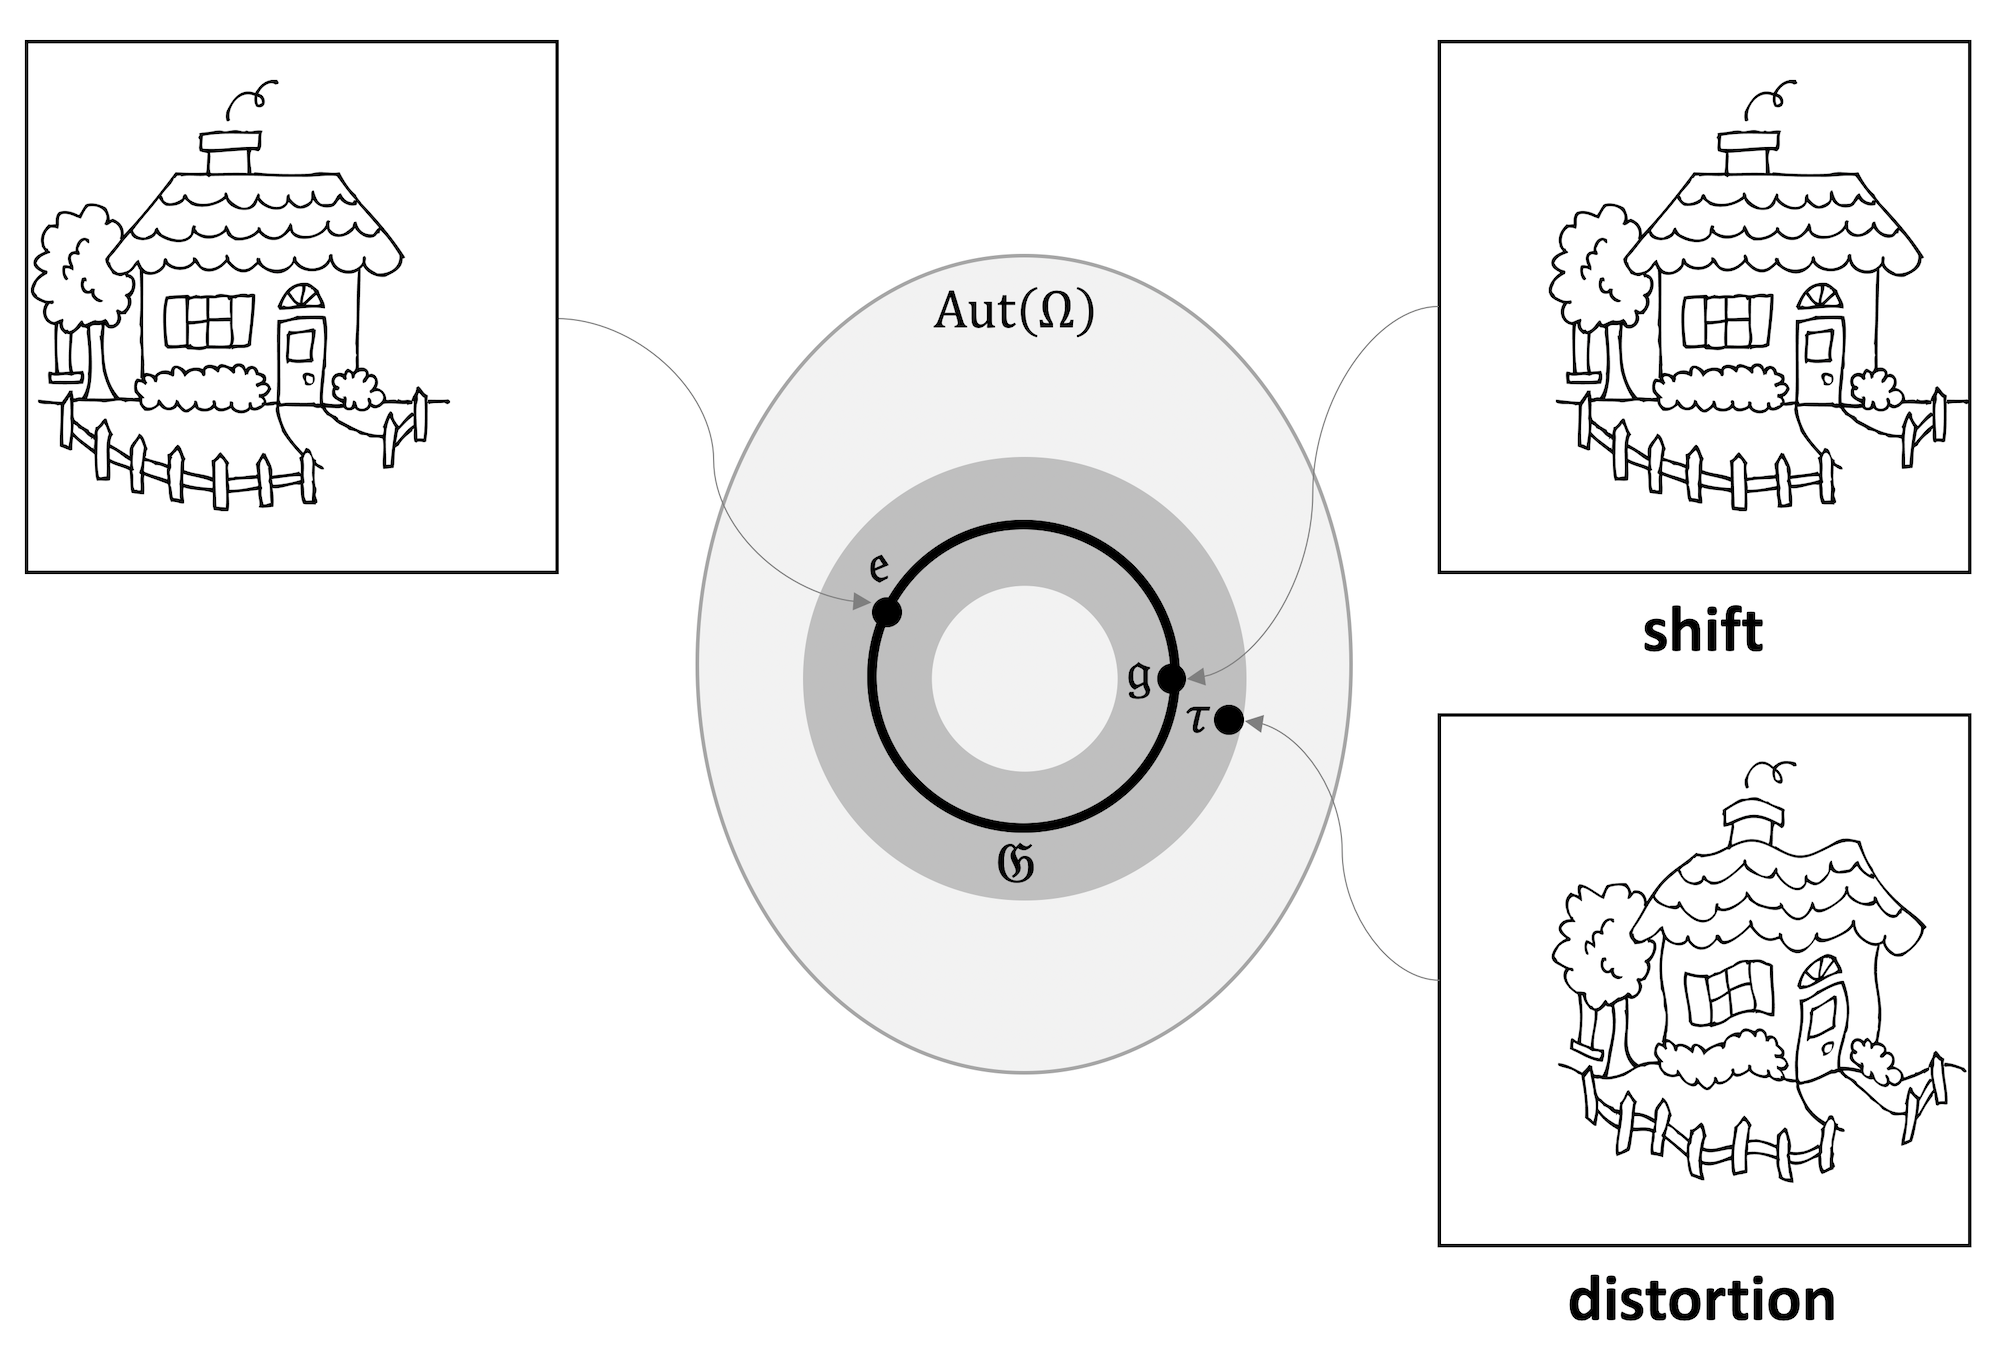
\includegraphics[width=1\textwidth]{figures/g_autg.png}
    \caption{The set of all bijective mappings from $\Omega$ into itself forms the \emph{set automorphism group}  $\mathrm{Aut}(\Omega)$, of which a symmetry group $\fG$ (shown as a circle) is a subgroup. Geometric Stability extends the notion of $\fG$-invariance and equivariance to `transformations around $\fG$' (shown as gray ring), quantified in the sense of some metric between transformations.
    In this example, a smooth distortion of the image is close to a shift. 
    }
    \label{fig:groupdeformation}
\end{figure}

%\begin{figure}
%    \centering
%    \includegraphics[width=0.7\textwidth]{figures/deform_image.pdf} \\
%    \includegraphics[width=0.7\textwidth]{figures/shapedef.pdf} \\
%        \includegraphics[width=0.4\textwidth]{figures/protein.jpg}
%    \caption{Examples of Deformations across different domains with a strong 
%    geometric stability prior. \michael{Better show a small molecule with a rotamer? Perhaps show just two examples of each?} }
%    \label{fig:deformation}
%\end{figure}

\paragraph{Stability to domain deformations}
In many applications, the object being deformed is not the signal, but the geometric domain $\Omega$ itself. Canonical instances of this are applications dealing with graphs and manifolds: a graph can model a social network at different instance of time containing slightly different social relations (follow graph), or a manifold can model a 3D object undergoing non-rigid deformations. 
%The intuition that one can slightly bend or twist a manifold can be formalized by considering a 
This deformation can be quantified as follows. If $\mathcal{D}$ denotes the space of all possible variable domains (such as the space of all graphs, or the space of Riemannian manifolds), one can define for $\Omega, \tilde{\Omega} \in \mathcal{D}$   an appropriate metric (`distance') $d(\Omega, \tilde{\Omega})$ satisfying $d(\Omega,\tilde{\Omega})=0$ if $\Omega$ and $\tilde{\Omega}$ are equivalent in some sense: for example, the graph edit distance vanishes when the graphs are isomorphic, and the Gromov-Hausdorff distance between Riemannian manifolds equipped with geodesic distances vanishes when two manifolds are isometric.\marginnote{The graph edit distance measures the minimal cost of making two graphs isomorphic by a sequences of graph edit operations. The Gromov-Hausdorff distance measures the smallest possible metric distortion of a correspondence between two metric spaces, see \cite{gromov1981structures}. } 


A common construction of such distances between domains relies on some family of 
%We assume that this metric comes with an 
invertible mapping $\eta: \Omega \to \tilde{\Omega}$ that try to `align' the domains in a way that the corresponding structures are best preserved. %This can be quantified for, %that is,
For example, in the case of graphs or Riemannian manifolds (regarded as metric spaces with the geodesic distance), this alignment can compare pair-wise adjacency or distance structures ($d$ and $\tilde{d}$, respectively),  %the alignment of graphs
%two graphs with $n$ nodes can be aligned 
%
$$d_{\gD}(\Omega, \tilde{\Omega}) =  \inf_{\eta \in \fG}\|d - \tilde{d}\circ (\eta \times \eta)\|$$
%
%$$d(\Omega, \Omega') = \inf_{\eta \in \fG} %\| e(\Omega) - \eta e(\Omega') \|~,$$
where $\fG$ is the group of isomorphisms such as bijections or isometries, and the norm is defined over the product space $\Omega \times \Omega$. In other words, a distance between elements of $\Omega,\tilde{\Omega}$ is `lifted' to a distance between the domains themselves, by accounting for all the possible alignments that preserve the internal structure.   
%rigid 
%symmetries of the domain 
%(e.g. permutations for graphs, or isometries for Riemannian manifolds), and $e(\cdot)$ is an embedding of the domain (such as the adjacency matrix for a graph, or an Euclidean embedding for a manifold). 
%\michael{Joan: please check. The assumptions on $\eta$ e.g. in GH-metric are very weak, just a bijection}
\marginnote{Two graphs can be aligned by the Quadratic Assignment Problem (QAP), which considers in its simplest form two graphs $G,\tilde{G}$ of the same size $n$, and solves $\min_{\mathbf{P} \in \Sigma_n} \mathrm{trace}(\mathbf{A P \tilde{A} P}^\top)$, where $\mathbf{A}, \tilde{\mathbf{A}}$ are the respective adjacency matrices and $\Sigma_n$ is the group of $n \times n$ permutation matrices. The graph edit distance can be associated with such QAP \citep{bougleux2015quadratic}.
}
Given a signal $x \in \gX(\Omega)$ and a deformed domain $\tilde{\Omega}$, one can then consider the deformed signal $\tilde{x} = x \circ \eta^{-1} \in \gX(\tilde{\Omega})$. 
%, $x' := x \circ \varphi^{-1}$.  
%For example, we can define a metri

%metric \emph{in the space of domains}. In other words, two graphs %$G, G'$ can be assigned a distance $d(G,G')$ so that $d(G,G')=0$ iff $G$ and $G'$ are isomorphic, and similarly two Riemannian manifolds $\Omega, \Omega'$ can be compared so that $d(\Omega, \Omega')$ measures the changes in their intrinsic metric structure. 

By slightly abusing the notation, we define $\gX(\mathcal{D}) = \{ (\gX(\Omega), \Omega) \, : \, \Omega \in \mathcal{D} \}$ as the ensemble of possible input signals defined over a varying domain. 
A function $f : \gX(\mathcal{D}) \to \gY$ is stable to domain deformations if 
\begin{equation}
\| f( x, \Omega) - f(\tilde{x}, \tilde{\Omega}) \| \leq C \|x \| d_{\gD}(\Omega, \tilde{\Omega})~
\label{eqn:domain_def_stability}
\end{equation}
%
for all $\Omega, \tilde{\Omega} \in \mathcal{D}$, and  $x \in \mathcal{X}(\Omega)$. 
%
%\michael{This is not properly defined: we have $x$ defined on both $\Omega$ and $\Omega'$, which requires some notion of correspondence} \joan{added some clarifications}. 
We will discuss this notion of stability in the context of manifolds in Sections~\ref{sec:manifolds}--\ref{sec:meshes}, where isometric deformations play a crucial role.
%As we will see in Chapter ??, 
Furthermore, it can be shown that the stability to domain deformations is a natural generalisation of the stability to signal deformations, by viewing the latter in terms of deformations of the volume form \cite{gama2019diffusion}. 

% %Link between the two via a change of variables. 
% In fact, the two notions of deformation stability are intimately related. Indeed, the deformation operator $L_\tau : \gX \to \gX$ acting on signals can be recast as deforming the inner-product metric, from $\gX = L^2(\Omega, du)$ to $L^2(\Omega,du_\tau)$. In other words, 
% $$\langle L_\tau x, L_\tau y \rangle_{L^2(\Omega), du)} = \int_\Omega x(\tau^{-1}(u)) y(\tau^{-1}(u)) du = \int_\Omega x(u) y(u) |\mathbf{I} - \nabla \tau^{-1}(u) | du := \int_\Omega x(u) y(u) du_\tau~,$$
% so we may view certain signal deformations as specific perturbations of the metric. 

%\michael{Measure not metric? or volume form? I find this section more confusing than helpful, we need to introduce a lot of extra stuff to make it defined properly} \joan{yes, agreed, i simply put a pointer for the future chapter to simplify things for now}. 



\subsection{Scale Separation}
\label{sec:scale_separation}

While deformation stability substantially strengthens the global symmetry priors, it is not sufficient in itself to overcome the curse of dimensionality, in the sense that, informally speaking, there are still ``too many" functions that respect (\ref{eq:defstability1}) as the size of the domain grows. A key insight to overcome this curse is to exploit the multiscale structure of physical tasks. Before describing multiscale representations, we need to introduce the main elements of Fourier transforms, which rely on frequency rather than scale. 

\paragraph{Fourier Transform and Global invariants}
Arguably 
\marginnote{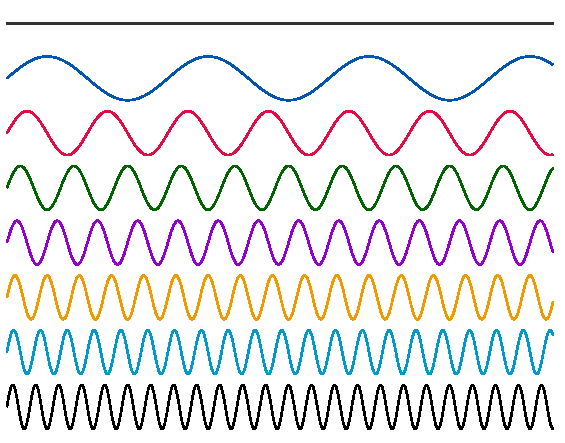
\includegraphics[width=\linewidth]{figures/fourier_basis.pdf}
Fourier basis functions have global support. As a result, local signals produce energy across all frequencies. 
}
the most famous signal decomposition is the {\em Fourier transform}, the cornerstone of harmonic analysis. 
%
The classical one-dimensional Fourier transform  
$$
\hat{x}(\xi) = \int_{-\infty}^{+\infty} x(u) e^{-\mi \xi u} \mathrm{d}u
$$
expresses the function $x(u) \in L^2(\Omega)$ on the domain $\Omega = \mathbb{R}$ as a linear combination 
of orthogonal oscillating {\em basis functions} $\varphi_\xi(u) = e^{\mi\xi u}$, 
indexed 
by their rate of oscillation (or \emph{frequency}) $\xi$. Such an organisation into frequencies reveals important information about the signal, e.g. its smoothness and localisation. 
%
%As we will show in Chapter ??, 
The Fourier basis itself has a deep geometric foundation and can be interpreted as the natural vibrations of the domain, related to its geometric structure (see e.g. \cite{berger2012panoramic}). 
%\marginnote{Technically, the Fourier transform is defined for functions in $L^2(\Omega) \cup L^1(\Omega)$, and can be extended to a far broader class of generalised functions through the theory of {\em tempered distributions} developed by the Fields laureate Laurent Schwartz. 
%We refer to \cite{mckean} for a wonderful treatment of Fourier Analysis

%

%\begin{figure}
%    \centering
%\includegraphics[width=0.5\linewidth]{figures/fourier1.pdf}
%    \caption{Basic decomposition of a signal into Fourier atoms. Observe that a localized discontinuity in the original signal produces energy across all frequencies.}
%    \label{fig:fourier}
%\end{figure}


%

% \joan{Michael, let me know if you agree. The following paragraph is not strictly needed in this section, and rather belongs to the grid/euclidean domain where we go again through this. I suggest we merge in there.} 
The Fourier transform\marginnote{In the following, we will use convolution and {\em (cross-)correlation} 
$$
(x \, \star \,\theta)(u) = \int_{-\infty}^{+\infty} \hspace{-2mm} x(v)\theta(u+v) \mathrm{d}v
$$
interchangeably, as it is common in machine learning: the difference between the two is whether the filter is reflected, and since the filter is typically learnable, the distinction is purely notational.
} plays a crucial role in signal processing as it offers a dual formulation of {\em convolution}, 
$$
(x\star \theta)(u) = \int_{-\infty}^{+\infty} x(v)\theta(u-v) \mathrm{d}v
$$
a standard model of linear signal filtering (here and in the following, $x$ denotes the signal and $\theta$ the filter). 
%
As we will show in the following, the convolution operator is diagonalised in the Fourier basis, making it possible to express convolution as the product of the respective Fourier transforms, 
$$
\widehat{(x\star \theta)}(\xi) = \hat{x}(\xi) \cdot \hat{\theta}(\xi),
$$
a fact known in signal processing as the Convolution Theorem. 
%
%In machine learning, convolution is the cornerstone of Convolutional Neural Networks, an architecture ubiquitously used in computer vision and image analysis applications. 


%Some of the properties of the Fourier transform are intimately related to the geometric properties of the Euclidean space or a grid on which it is defined.    
%The Fourier basis thus diagonalises any convolutional operator. 
As it turns out, many fundamental differential operators such as the Laplacian are described as convolutions on Euclidean domains. 
%, such as the Laplacian $\Delta = \mathrm{div} \, \nabla$. 
Since such differential operators can be defined intrinsically  over very general geometries, this provides a formal procedure to extend Fourier transforms beyond Euclidean domains, including graphs, groups and manifolds. We will discuss this in detail in Section~\ref{sec:manifolds}. %Chapter~???.

An essential aspect of Fourier transforms is that they reveal \emph{global} properties of the signal and the domain, such as smoothness or conductance. Such global behavior is convenient in presence of global symmetries of the domain such as translation, but not to study more general diffeomorphisms. This requires a representation that trades off spatial and frequential localisation, as we see next. 


\paragraph{Multiscale representations}
The 
%\marginnote{
%\includegraphics[width=0.9\linewidth]{figures/wavelet.pdf}
%Basic decomposition of a signal into wavelet atoms. Observe that now a localized discontinuity in the original signal creates energy only in the neighborhood of the discontinuity. 
notion of local invariance can be articulated by switching from a Fourier frequency-based representation to a {\em scale-based} representation, the cornerstone of multi-scale decomposition methods such as {\em wavelets}.\marginnote{See \cite{mallat1999wavelet} for a comperehensive introduction. } 
%; see Figure \ref{fig:fourier_vs_wavelets} and Insert ??. 
%
The essential insight of multi-scale methods is to decompose functions defined over the domain $\Omega$ into elementary functions that are localised \emph{both in space and frequency}.\marginnote{
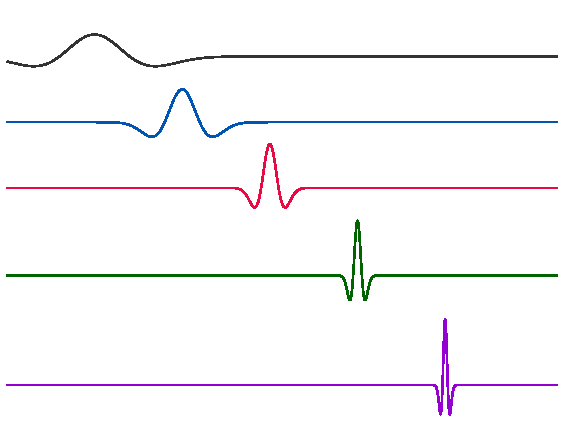
\includegraphics[width=0.9\linewidth]{figures/wavelet_basis.pdf}
%\includegraphics[width=0.9\linewidth]{figures/wavelet.pdf}
Contrary to Fourier, wavelet atoms are localised and multi-scale, allowing to capture 
fine details of the signal with atoms having small spatial
support and coarse details with atoms having large
spatial support.  
%Localized signals create energy only in the neighborhood of the discontinuity. 
The term \emph{ atom} here is synonymous with `basis element' in Fourier analysis, with the caveat that wavelets are redundant (over-complete).
}
In the case of wavelets, this is achieved by correlating a translated and dilated filter ({\em mother wavelet}) $\psi$, producing a combined spatio-frequency representation called a  {\em continuous wavelet transform} 
%
$$
(W_\psi x)(u,\xi) = \xi^{-1/2} \int_{-\infty}^{+\infty} 
\psi\left(\frac{v-u}{\xi}\right) x(v) \mathrm{d}v.
%psi( 2^{j} (u - k2^{-j})) 
%x(u) du \marginnote{In general, $\psi$ can be a complex-valued function, in which case a complex conjugation must be taken in the inner product.}
%(x \star \psi_j)(u)
$$
%
The translated and dilated filters are called {\em wavelet atoms}; % \marginnote{The term \emph{ atom} here is synonymous with `basis element' in Fourier analysis, with the caveat that wavelets are redundant representations that form over-complete bases.}
their spatial position and dilation correspond to the coordinates $u$ and $\xi$ of the wavelet transform. 
%
These coordinates are usually sampled dyadically ($\xi=2^{-j}$ and $u = 2^{-j}k$), with $j$ referred to as {\em scale}.  
%
%
%\int_{-\infty}^{+\infty} 
%\psi( 2^{j} (u - k2^{-j})) 
%x(u) du \marginnote{In general, $\psi$ can be a complex-valued function, in which case a complex conjugation must be taken in the inner product.}
%(x \star \psi_j)(u)
%$$
%
Multi-scale signal representations bring important benefits in terms of capturing regularity properties beyond global smoothness, such as piece-wise smoothness, which made them a popular tool in signal and image processing and numerical analysis in the 90s. 

\paragraph{Deformation stability of Multiscale representations:}
The benefit of multiscale localised wavelet decompositions over Fourier decompositions is revealed when considering the effect of small deformations `nearby' the underlying symmetry group. Let us illustrate this important concept in the Euclidean domain and the translation group.   
Since the Fourier representation diagonalises the shift operator (which can be thought of as convolution, as we will see in more detail in  Section~\ref{sec:grids_euclidean}), it is an efficient representation for translation transformations. However, Fourier decompositions are unstable under high-frequency deformations. 
%
In contrast, wavelet decompositions offer a stable representation in such cases. 

Indeed, let us consider $\tau \in \mathrm{Aut}(\Omega)$ and its associated linear representation $\rho(\tau)$. When $\tau(u) = u - v$ is a shift, 
as we will verify in Section \ref{sec:grids_euclidean}, the operator $\rho(\tau) = S_v$ is a {\em shift operator} that commutes with convolution. 
%any convolution operator $H$ of the form $H x = x \star h$, with arbitrary filter $h$. 
Since convolution operators are diagonalised by the Fourier transform, the action of shift in the frequency domain amounts to shifting the complex phase of the Fourier transform,  
%
%As a result, by expressing this commutation relationship in the Fourier domain, we have that 
$$
(\widehat{S_v x})(\xi) = e^{-\mi \xi v} \hat{x}(\xi). 
$$ 
%for any frequency $\xi$. 
%Rigid translations are thus expressed in the Fourier domain by simply shifting the (complex) phase of every fourier coefficient of the signal, leading 
Thus, the {\em Fourier modulus} $f(x) = |\hat{x}|$ removing the complex phase is a simple shift-invariant function, $f(S_v x) = f(x)$. 
%to simple translation invariant representations by removing this complex phase: $Mx = |\hat{x}|$. In other words, for rigid translations, the Fourier modulus is translation invariant: $\| M - M L_\tau \| = 0$. 
%
However, if we have only approximate translation, 
%$\tau(u) \approx u - v$, 
$\tau(u) = u - \tilde{\tau}(u)$ with $\|\nabla \tau \|_\infty = \sup_{u\in \Omega} \| \nabla \tilde{\tau}(u)\| \leq \epsilon$,  
the situation is entirely different: it is possible to show that 
$$
\frac{\|f(\rho(\tau) x) - f(x) \| }{ \|x\| }= \mathcal{O}(1)
$$ 
irrespective of how small $\epsilon$ is (i.e., how close is $\tau$ to being a shift). Consequently, such Fourier representation is {\em unstable under deformations}, however small. This unstability is manifested in general domains and non-rigid transformations; we will see another instance of this unstability in the analysis of 3d shapes using the natural extension of Fourier transforms described in Section \ref{sec:geomanifoldsec}. 

Wavelets offer a remedy to this problem that also reveals the power of multi-scale representations. In the above example, we can show \citep{mallat2012group} that the wavelet decomposition $W_\psi x$ is {\em approximately equivariant} to deformations,
$$
\frac{\| \rho(\tau) (W_\psi x) - W_\psi (\rho(\tau) x) \|}{\|x\|} = \mathcal{O}(\epsilon).
\marginnote{This notation implies that $\rho(\tau)$ acts on the spatial coordinate of $(W_\psi x)(u,\xi)$.
}
$$
%and $\gW x = \{ x \star \psi_j \}_j$ is an appropriately normalized wavelet filter bank, then one can verify that wavelet coefficients are nearly \emph{equivariant} to deformations, in the sense that $\| L_\tau \gW - \gW L_\tau \| = O(\epsilon)$. 
%
In other words, decomposing the signal information into scales using localised filters rather than frequencies turns a global unstable representation into a family of locally stable features. Importantly, such measurements at different scales are not yet invariant, and need to be progressively processed towards the low frequencies, hinting at the deep compositional nature of modern neural networks, and captured in our Blueprint for Geometric Deep Learning, presented next. 


% From our discussion 
% Let us consider a filter $h(u)$ and its associated convolution operator $\gH x = x \star h$. To study how this operator behaves under certain geometric transformations $L_\tau \in \mathrm{Aut}(\Omega)$ we consider the \emph{Lie commutator} 

% Let us consider the Lie commutator $[L_\tau, \gW]= L_\tau \gW - \gW L_\tau$. When $\gW$ is the Fourier transform and $L_\tau$ is exactly a translation, we have $[L_\tau, \gW] = 0$; 
% %Let us denote the decomposition by $U$ and let $L_\tau$ be the deformation operator we have seen before. When $\tau(u) = u-v$ is a pure translation, the Fourier transform satisfies $L_\tau U = U L_\tau$, by virtue of its 
% however when $L_\tau$ is only an approximate translation, then $\| [L_\tau, \gW] \| = O(1)$, irrespective of how close $L_\tau$ is to being a translation. 
% On the other hand, if $\tau(u) = u - \tilde{\tau}(u)$, with $\sup_u \| \nabla \tilde{\tau}(u)\| \leq \epsilon$ (thus $\tau$ is nearly a translation), then one can show \cite{scatt} that when $\gW$ is the overcomplete wavelet transform, $\| [ L_\tau, \gW ] \| \simeq \epsilon$. 





%\paragraph{Scale Separation}
%In our context of high-dimensional learning, multiscale representations such as wavelets serve another fundamental purpose: they provide overcomplete linear decompositions where local translations are nearly equivariant.  
\paragraph{Scale Separation Prior: }
We can build from this insight by considering a multiscale coarsening of the data domain $\Omega$ into a hierarchy $\Omega_1, \hdots, \Omega_J$. 
%, $j\in [J]$. 
As it turns out, such coarsening can be defined on very general domains, including grids, graphs, and manifolds. 
%capturing a wide range of applications.
Informally, a coarsening assimilates nearby points $u, u' \in \Omega$ together, and thus only requires an appropriate notion of {\em metric} in the domain. 
%Geometric objects such as grids, manifolds, Lie groups or Graphs all admit such coarsenings. 
If $\gX_{j}(\Omega_j,\mathcal{C}_j) := \{x_j: \Omega_j \to \mathcal{C}_j \}$ 
%\michael{\bf [MB: why $\R^s$? did not we assume scalar-valued signals for simplicity? ]} 
%\joan{JB: number of channels can vary as we coarsen the domain. But we should keep things simple at this stage, and just describe the general principle without introducing too much notation. } \michael{MB: lets keep it as simple as possible here} 
denotes signals defined over the coarsened domain $\Omega_j$, we informally say that a function $f : \gX(\Omega) \to \gY$ is \emph{locally stable} at scale $j$ if it admits a factorisation of the form $f \approx f_j \circ P_j $, where $P_j : \gX(\Omega) \to \gX_{j}(\Omega_j)$ is a non-linear \emph{coarse graining} and $f_j : \gX_{j}(\Omega_j) \to \gY$. In other words, while the target function $f$ might depend on complex long-range interactions between features over the whole domain, in locally-stable functions it is possible to \emph{separate} the interactions across scales, by first focusing on localised interactions that are then propagated towards the coarse scales. 

\begin{figure}
    \centering
    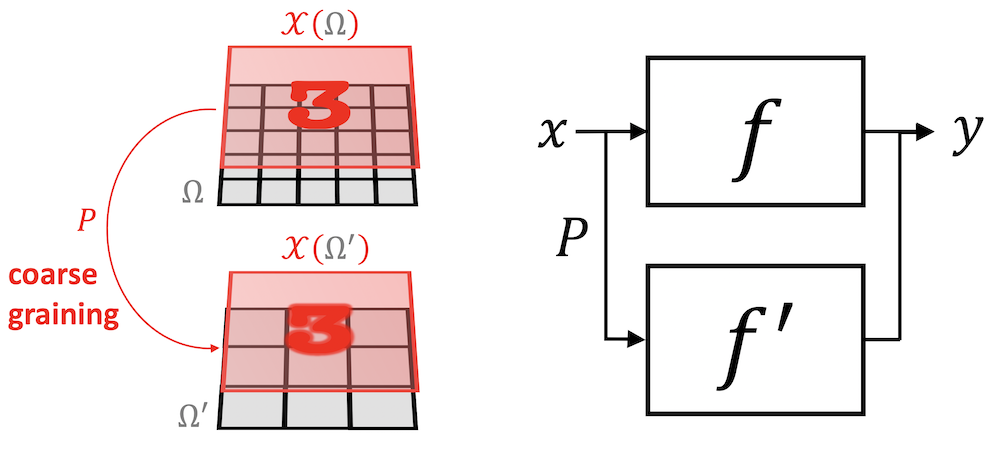
\includegraphics[width=0.75\textwidth]{figures/scale_sep.png}%factorization.pdf}
    \caption{Illustration of Scale Separation for image classification tasks. The classifier $f'$ defined on signals on the coarse grid $\mathcal{X}(\Omega')$ should satisfy $f \approx f'\circ P$, where $P: \mathcal{X}(\Omega) \rightarrow \mathcal{X}(\Omega')$. }
    \label{fig:scale_separation}
\end{figure}

Such principles\marginnote{Fast Multipole Method (FMM) is a numerical technique originally developed to speed up the calculation of long-ranged forces in $n$-body problems. FMM groups sources that lie close together and treats them as a single source.
} are of fundamental importance in many areas of physics and mathematics, as manifested for instance in statistical physics in the so-called renormalisation group, or leveraged in important numerical algorithms such as the Fast Multipole Method. In machine learning, multiscale representations and local invariance are the fundamental mathematical principles underpinning the efficiency of Convolutional Neural Networks and Graph Neural Networks and are typically implemented in the form of {\em local pooling}. In future work, we will further develop tools from computational harmonic analysis that unify these principles across our geometric domains and will shed light onto the statistical learning benefits of scale separation. 





\subsection{The Blueprint of Geometric Deep Learning}
\label{sec:gdl_blueprint}

The geometric principles of Symmetry, Geometric Stability, and Scale Separation discussed in Sections~\ref{sec:symmetries}--\ref{sec:scale_separation} can be combined to provide a universal blueprint for learning stable representations of high-dimensional data. 
%
These representations will be produced by functions $f$ operating on signals $\mathcal{X}(\Omega,\mathcal{C})$ defined on the domain $\Omega$, which is endowed with a symmetry group $\fG$. 


The geometric priors we have described so far do not prescribe a specific {\em architecture} for building such representation, but rather a series of necessary conditions. 
However, they hint at an axiomatic construction that provably satisfies these geometric priors, while ensuring a highly expressive representation that can approximate any target function satisfying such priors. %the geometric priors. 


A simple initial observation is that, in order to obtain a highly expressive representation, we are required to introduce a non-linear element, since
if $f$ is linear and $\fG$-invariant, then for all $x \in \gX(\Omega)$, \marginnote{Here, $\mu(\fg)$ is known as the \emph{Haar measure} of the group $\fG$, and the integral is performed over the entire group.}
$$
f(x) =  \frac{1}{\mu(\fG)} \int_{\fG} f( \fg. x) \mathrm{d}\mu(\fg) = f\left(\frac{1}{\mu(\fG)} \int_{\fG} (\fg.x) \mathrm{d}\mu(\fg) \right),
$$
%\michael{f(x) and not F?}
%\michael{what is $\fg.x$? should be u or use representation $\rho$}
which indicates that $F$ only depends on $x$ through the  \emph{$\fG$-average} $A{x} = \frac{1}{\mu(\fG)} \int_{\fG} (\fg.x) \mathrm{d}\mu(\fg)$. In the case of images and translation, this would entail using only the average RGB color of the input! %\marginnote{Give a further example for the discrete permutation group, getting the average too}


While this reasoning shows that the family of {\em linear invariants} is not a very rich object, the family of {\em linear equivariants} provides a much more powerful tool, since it enables the construction of rich and stable features by composition with appropriate non-linear maps, as we will now explain. 
%
Indeed, if $B: \gX(\Omega, \gC) \to \gX( \Omega, \gC')$ is $\fG$-equivariant satisfying $B(\fg.x) = \fg.B(x)$ for all $x \in \gX$ and $\fg \in \fG$, and $\sigma: \gC' \to \gC''$ is an arbitrary (non-linear) map, then we easily verify that the composition $U := (\bm{\sigma} \circ B): \gX(\Omega, \gC) \to \gX( \Omega, \gC'')$ is also $\fG$-equivariant, where $\bm{\sigma}: \gX(\Omega,\gC') \to \gX(\Omega, \gC'')$ is the element-wise instantiation of $\sigma$ given as $(\bm{\sigma}(x))(u) := \sigma( x(u))$.

This simple property allows us to define a very general family of $\fG$-invariants, by composing $U$ with the group averages $A \circ U : \gX(\Omega, \gC) \to \gC''$. A natural question is thus whether any $\fG$-invariant function can be approximated at arbitrary precision by such a model, for appropriate choices of $B$ and $\sigma$. 
%
It is not hard to adapt the standard Universal Approximation Theorems from unstructured vector inputs to show that shallow `geometric' networks are also universal approximators, by properly generalising the group average to a general non-linear invariant. 
\marginnote{Such proofs have been demonstrated, for example, for the Deep Sets model by \citet{zaheer2017deep}.}
%
However, as already described in the case of Fourier versus Wavelet invariants, there is a 
fundamental tension between shallow global invariance and deformation stability.
This motivates an alternative representation, which considers instead \emph{localised} equivariant maps.\marginnote{Meaningful metrics can be defined on grids, graphs, manifolds, and groups. A notable exception are sets, where there is no predefined notion of metric. 
%; see Section ? for further discussion.
} 
Assuming that $\Omega$ is further equipped with a distance metric $d$, we call an equivariant map $U$ localised if $(Ux)(u)$ depends only on the values of $x(v)$ for $\mathcal{N}_u = \{v : d(u,v) \leq r\}$, for some small radius $r$; the latter set $\mathcal{N}_u$ is called the {\em receptive field}. %$\delta$; . 
%\michael{Are we ok to indentify neighbourhood with receptive field?}

A single layer of local equivariant map $U$ cannot approximate functions with long-range interactions, but a composition of several local equivariant maps $U_J \circ U_{J-1} \dots \circ U_1$ increases the receptive field\marginnote{The term `receptive field' originated in the  neuroscience literature, referring to the spatial domain that affects the output of a given neuron.}  while preserving the stability properties of local equivariants. The receptive field is further increased by interleaving downsampling operators that coarsen the domain (again assuming a metric structure), completing the parallel with Multiresolution Analysis (MRA, see e.g. \cite{mallat1999wavelet}). 

\begin{figure}
    \centering
    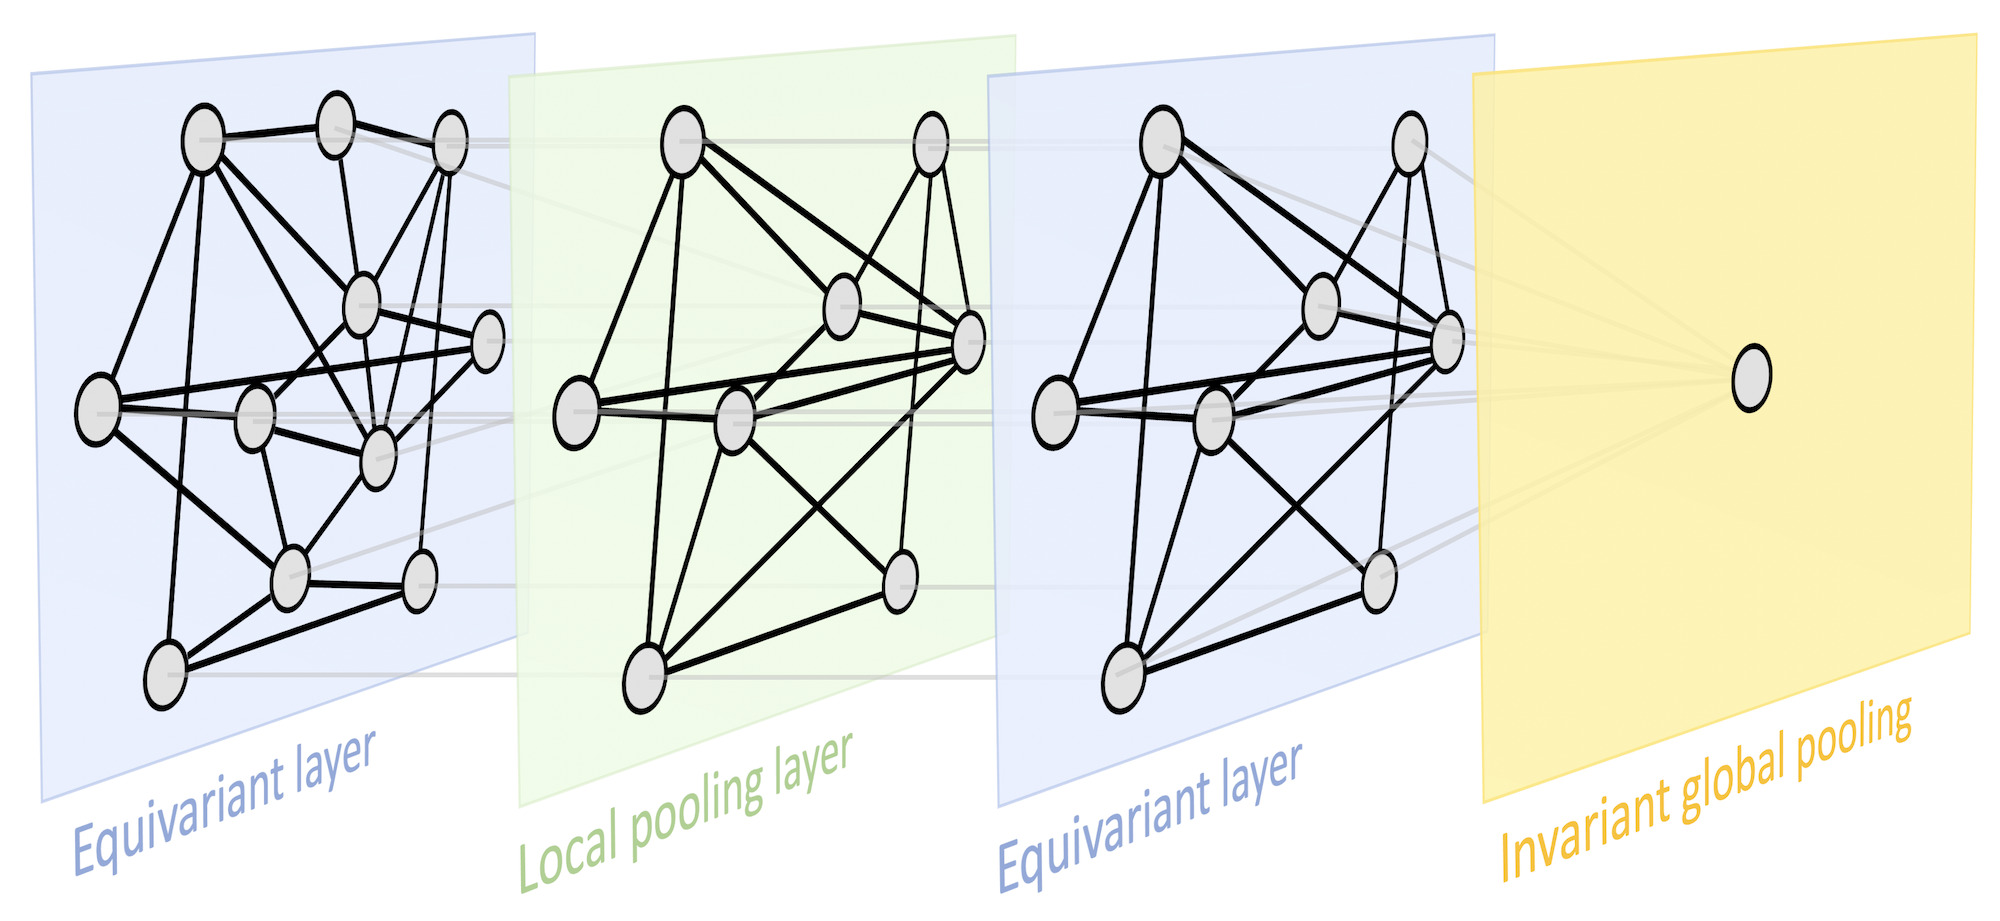
\includegraphics[width=1\textwidth]{figures/blueprint.png}
    \caption{Geometric Deep Learning blueprint, exemplified on a graph. A typical Graph Neural Network architecture may contain permutation equivariant layers (computing node-wise features), local pooling (graph coarsening), and a permutation-invariant global pooling layer (readout layer). }
    \label{fig:blueprint}
\end{figure}

In summary, the geometry of the input domain, with knowledge of an underyling symmetry group, provides three key building blocks: (i) a local equivariant map, (ii) a global invariant map, and (iii) a coarsening operator. These building blocks provide a rich function approximation space with prescribed invariance and stability properties by combining them together in a scheme we refer to as the  
%
\emph{Geometric Deep Learning Blueprint} (Figure~\ref{fig:blueprint}). 
%
%We will see that a large number of popular neural network architectures used in deep representation learning are particular instances of this blueprint, illustrated in 
%across all the geometric domains we will describe next. 
%



%\begin{tcolorbox}[width=\linewidth,
%                  boxsep=0pt,
%                  left=7.5pt,
%                  right=7.5pt,
%                  top=7.5pt,
%                  bottom=7.5pt,
%                  arc=0pt,
%                  boxrule=0pt,toprule=0pt,
%                  colback=boxgray,
%                  ]%%
    
%\begin{center}
%Given a hierarchy of domains $\Omega_J \subseteq \hdots \subseteq \Omega_2 \subseteq \Omega_1 = \Omega$ with symmetry group $\fG$, the 
%\textbf{Geometric Deep Learning Blueprint} allows constructing $\fG$-invariant functions $f:\mathcal{X}(\Omega,\mathcal{C}) \rightarrow \mathcal{Y}$ of the form 
%$$
%f = A \circ \boldsymbol{\sigma}_J \circ U_J \circ P_{J-1} \circ \hdots \circ P_1 \circ \boldsymbol{\sigma}_1 \circ B_1
%$$
%consisting  of the following building blocks:\\

%    \noindent {\em Linear $\fG$-equivariant layer} $B_j: \gX(\Omega_j, \gC_j) \to \gX( \Omega_{j}, \gC'_{j})$ satisfying $B(\fg.x) = \fg.B(x)$ for all $\fg \in \fG$ and $x\in \gX(\Omega_j,\mathcal{C}_j)$. 
%    \vspace{2mm}\\

%    \noindent {\em Nonlinearity} $\sigma_j: \gC'_j \to \gC_j$ applied element-wise as $(\bm{\sigma}(x))(u) = \sigma( x(u))$.\vspace{2mm}\\\

%    \noindent {\em Local pooling (coarsening)}  $P_j : \gX(\Omega_j, \gC_j) \rightarrow \gX(\Omega_{j+1}, \gC_{j+1}) $.\vspace{2mm}\\
    
%    \noindent {\em Invariant layer (global pooling) } $A: \gX(\Omega_J, \gC_J) \rightarrow \mathcal{Y}$ satisfying $A(\fg .x) = A(x)$ for all $\fg \in \fG$ and $x\in \gX(\Omega_J,\mathcal{C}_J)$.  %.\vspace{2mm}\\

%\end{center}
%\end{tcolorbox}


\begin{tcolorbox}[width=\linewidth,
                  boxsep=0pt,
                  left=7.5pt,
                  right=7.5pt,
                  top=7.5pt,
                  bottom=7.5pt,
                  arc=0pt,
                  boxrule=0pt,toprule=0pt,
                  colback=boxgray,
                  ]%%
    
\begin{center}
\textbf{Geometric Deep Learning Blueprint}
\end{center}
Let $\Omega$ and $\Omega'$ be domains, $\fG$ a symmetry group over $\Omega$, and write $\Omega' \subseteq \Omega$ if $\Omega'$ can be considered a compact version of $\Omega$. \\

We define the following building blocks:\vspace{2mm}\\

    \noindent {\em Linear $\fG$-equivariant layer} $B: \gX(\Omega, \gC) \to \gX( \Omega', \gC')$ satisfying $B(\fg.x) = \fg.B(x)$ for all $\fg \in \fG$ and $x\in \gX(\Omega,\mathcal{C})$.\vspace{2mm}\\

    \noindent {\em Nonlinearity} $\sigma: \gC \to \gC'$ applied element-wise as $(\bm{\sigma}(x))(u) = \sigma( x(u))$.\vspace{2mm}\\

    \noindent {\em Local pooling (coarsening)}  $P : \gX(\Omega, \gC) \rightarrow \gX(\Omega', \gC) $, such that $\Omega'\subseteq\Omega$.\vspace{2mm}\\
    
    \noindent {\em $\fG$-invariant layer (global pooling) } $A: \gX(\Omega, \gC) \rightarrow \mathcal{Y}$ satisfying $A(\fg .x) = A(x)$ for all $\fg \in \fG$ and $x\in \gX(\Omega,\mathcal{C})$.\vspace{2mm}\\

Using these blocks allows constructing $\fG$-invariant functions $f:\mathcal{X}(\Omega,\mathcal{C}) \rightarrow \mathcal{Y}$ of the form 
$$
f = A \circ \boldsymbol{\sigma}_J \circ B_J \circ P_{J-1} \circ \hdots \circ P_1 \circ \boldsymbol{\sigma}_1 \circ B_1
$$
where the blocks are selected such that the output space of each block matches the input space of the next one. Different blocks may exploit different choices of symmetry groups $\fG$.
\end{tcolorbox}

%


% A natural question is then how expressive this generic construction is in the class of $\fG$-invariant functions, and, equally important, which conditions on $B$ and $\rho$ ensure geometric stability.  
% Universal Approximation

% A simple option to ensure rich and stable representations is to instead compose several \emph{layers} of non-linear local equivariant maps before applying the global invariant. 

% The idea of deep learning is to define $f$ as a \emph{composition} of maps (or ``layers'').
% These maps should be compatible in that the output space of one layer should match the input space of the next layer.
% %That is, we can compose $f_1 : \mathcal{X}(\Omega, \mathcal{C}) \rightarrow \mathcal{X}(\Omega', \mathcal{C}')$ and $f_2 : \mathcal{X}(\Omega'', \mathcal{C}'') \rightarrow \mathcal{X}(\Omega''', \mathcal{C}''')$ if and only if $\mathcal{X}(\Omega', \mathcal{C}') = \mathcal{X}(\Omega'', \mathcal{C}'')$.
% That is, we can compose $f_1 : \mathcal{X}_1 \rightarrow \mathcal{X}_2$ and $f_2 : \mathcal{X}_2' \rightarrow \mathcal{X}_3$ if and only if $\mathcal{X}_2 = \mathcal{X}_2'$ (where we have abbreviated $\mathcal{X}_i = \mathcal{X}(\Omega_i, \mathcal{C}_i)$).
% Whereas in regular deep learning, maps can be composed as soon as the input and output spaces match as \emph{vector spaces} (i.e. they have the same dimensionality / array shape), in geometric deep learning these spaces should match as \emph{group representations}.
% This means that, in addition to matching as vector spaces, the group $\fG$ should act in the same way on both spaces.
% When this is the case, equivariance of $f_1$ and $f_2$ implies equivariance of the composition $f_2 \circ f_1$.

% Most networks in geometric deep learning are compositions of a few basic building blocks:

% %\emph{Local} 
% $\fG$-\emph{equivariant} linear operator $A: \gX(\Omega) \to \gX_{\gV'}(\Omega)$ satisfying $A(\fg.x) = \fg. A(x)$ for any $x \in \mathcal{X}(\Omega)$ and $\fg\in\fG$. 
% %
% Typically, this operator is further assumed to be {\em local}, i.e. $(Ax)(u)$ depends only on the values of $x(v)$ for $v$ in the vicinity of $u$, in the sense of some metric on $\Omega$.  
% %and such that $A x(u)$ only depends upon $\{ x(v); \mathrm{g}(v,u) \leq \delta\}$, where $\delta$ encodes the size of the neighborhood. 

% \emph{Pointwise nonlinearity} $\sigma: \mathcal{C}' \to \mathcal{C}''$. Under our assumptions, this implies that $\sigma \circ A$ is local and $\fG$-\emph{equivariant} whenever $A$ is such. \marginnote{When $\sigma$ acts coordinate-wise, it is typically referred to as an \emph{activation function}. In general,  $\sigma$ can be a generic function, such as a fully-connected neural network. }

% % \joan{
% % Argue that the only linear $\fG$-invariant is the group average. 
% % If $F$ is linear and $\fG$-invariant, then for all $x$, 
% % $$F(x) =  \frac{1}{\mu(\fG)} \int F( g.x) \mu(dg) = F\left(\frac{1}{\mu(\fG)} \int g.x \mu(dg) \right)~,$$
% % so $F$ only depends on $x$ through the average. 

% % This justifies why we need to add non-linearities
% % }




% {\em Local pooling} (or downsampling operator) $P_j: \gX(\Omega_j,\mathcal{C}_{j}) \to \gX(\Omega_{j+1},\mathcal{C}_{j+1})$ defined on a hierarchy of domains $\Omega_1, \hdots, \Omega_J$. 
% %reducing the resolution of the domain. 

% {\em Global pooling} $\fG$-{\em invariant} operator $a:\mathcal{X}(\Omega,\mathcal{C}) \rightarrow \mathcal{Y}$. 
    



% %
% %\michael{\bf [MB: INSERT FIGURE of a general equivariant/invariant architecture, similarly to Maron's thesis]}
% %
% %Let $\gX(\Omega, \gV) := \{ x : \Omega \to \gV \}$ be the input space, with domain $\Omega$ and feature space $\gV$ . We assume a metric $\mathrm{g}$ on $\Omega$ and a symmetry group $\fG$ acting on it, which also defines a linear representation 
% %%(taco confirm language? \taco{Correct. This is called the regular rep of G on X. Will add a definition to 1.2.1}) 
% %over $\gX$ by composition, as in Figure \ref{fig:symmetryactors}.
% %%if $x \in \gX$ and $g \in \fG$, then $g x (u) = x(gu) \in \R^s$. [we assume that the group does not act along channels for now]
% %\taco{TODO: add condition that signal space should have an inner product, i.e. be a Hilbert space. See definition box in 1.2}
% %
% %The GDL blueprint consists of four fundamental building blocks that are composed together appropriately:
% %\begin{enumerate}
% %    \item A \emph{local} $\fG$-\emph{equivariant} linear operator $A: \gX_{\gV}(\Omega) \to \gX_{\gV'}(\Omega)$; that is, $A(\fg.x) = \fg. A(x)$ for any $x$ and $\fg$, and such that $A x(u)$ only depends upon $\{ x(v); \mathrm{g}(v,u) \leq \delta\}$, where $\delta$ encodes the size of the neighborhood. 
% %    \item A \emph{nodewise} nonlinear activation function $\sigma: \gV' \to \gV''$. Under our assumptions, this implies that $\sigma \circ A$ is local and $\fG$-\emph{equivariant} whenever $A$ is as above. When $\text{dim}(\gV')=\text{dim}(\gV'')=1$, $\sigma$ is typically described as an \emph{activation function}, but in general $\sigma$ can be a generic function, such as a fully-connected neural network. 
% %    \item Local pooling or downsampling operator $P_k: \gX_{\gV}(\Omega_k) \to \gX_{\gV}(\Omega_{k+1})$ reducing the resolution of the domain. 
% %    \item Global pooling: $\fG$-invariant operator. 
% %\end{enumerate}




% %\michael{MB: I am in favor of keeping the blueprint as simple as possible even at the expense of precision of definitions/generality. It should be intuitive and I feel currently the intuition is buried under too much notation. }


% The majority of deep neural networks implement a composition of multiple such components of the form
% $$
% f =a \circ P_L \circ \sigma_L \circ A_L \dots P_1 \circ \sigma_1 \circ A_1,
% $$
% with each component referred to as a {\em layer}. The term `deep' is used to indicate that there are many such layers, though we should say that how deep is deep is in the eyes of the beholder.\marginnote{Some CNN architectures used in computer vision can have hundreds of layers. }
% %
% %The multilayer composition $f =a \circ P_L \circ \sigma_L \circ A_L \dots P_1 \circ \sigma_1 \circ A_1$ 
% %
% Such a multilayer construction allows to define a flexible functional space with prescribed geometric priors. On the one hand, the equivariant nature of the maps $\sigma \circ A_j$ is preserved under composition, resulting in overall invariance when composed with a global pooling operator. On the other hand, the use of pooling layers allows to exploit the scale separation prior. 

\paragraph{Different settings of Geometric Deep Learning}
One can make an important distinction between the setting when the domain $\Omega$ is assumed to be {\em fixed} and one is only interested in varying input signals defined on that domain, or the domain is part of the input as {\em varies} together with signals defined on it. 
%
A classical instance of the former case is encountered in computer vision applications, where images are assumed to be defined on a fixed domain (grid). 
%
Graph classification is an example of the latter setting, where both the structure of the graph as well as the signal defined on it (e.g. node features) are important. 
%
In the case of varying domain, geometric stability (in the sense of insensitivity to the deformation of $\Omega$) plays a crucial role in Geometric Deep Learning architectures. 


This blueprint  has the right level of generality to be used across a wide range of geometric domains. 
Different Geometric Deep Learning methods thus differ in their choice of the domain, symmetry group, and the specific implementation details of the aforementioned building blocks. 
%and the metric defining locality. 
As we will see in the following, a large class of deep learning architectures currently in use fall into this scheme and can thus be derived from common geometric principles.  
%
%We will now discuss specific instances of this blueprint and how it adapts to each case.  


In the following sections~(\ref{sec:proto-graphs}--\ref{sec:meshes}) we will describe the various geometric domains focusing on the `5G', and in Sections~\ref{sec:cnnsec}--\ref{sec:lstm} the  specific implementations of Geometric Deep Learning on these domains. 



%Such generic architecture, illustrated in Figure~\ref{fig:blueprint}, can be instantiated across a variety of domains with different geometric structures giving rise to a very large zoo of architectures united by these common geometric principles. Let us now discuss these domains and how this blueprint adapts to each case. 


% First, we define a collection of \emph{local} $\fG$-\emph{equivariant} linear operators. In  deep learning architectures such as CNNs and GNNs these correspond to convolutional and message passing layers, and the corresponding groups are translation and permutation, respectively. 

% Next, these operators are composed with a non-linearity called an {\em activation function} in the neural networks jargon, which preserves the equivariance as it is applied element-wise. \taco{TC: note that element-wise nonlinearities are only equivariant to certain kinds of group representations, namely when the representation matrices are all permutation matrices}

% Finally, coarsen the representations produced by the equivariant operators. In image analysis applications, this is achieved by means of {\em pooling}, an operation reducing the size of the image grid, and as we shall see next, coarsening may be defined on far more general data domains.

% In an idealised instantiation, the coarsening is performed at the output. It can be shown that this representation is 
% provably $\fG$-invariant/equivariant, and that the locality assumption captures the scale separation inductive bias. 
% Moreover, such representations are universal approximators under symmetry, as we discuss in Chapter ??. 

%\joan{Joan: Taco, we can generalise the blueprint to accommodate more group representations, if we feel the use cases are sufficiently important. Otherwise, an alternative is to mention that this blueprint can be extended in some domains to account for special types of group actions}

%\taco{Taco: Joan, I agree we really only need reps that describe how signals transform. However that is still a bit more general than $\rho(\fg) x(u) = x(\fg^{-1} u)$. In particular for steerable cnns / induced reps, as well as gauge cnns, we have some smaller group acting on the feature vector. E.g. a vector field on the sphere transforms according to the rep of SO3 that is induced by the vector rep of SO2 acting on 2D vectors. 

%One option is to ignore this for now and call this the ``deep learning blueprint (simplified)'', and mention that we need something slightly more general. We can introduce the full thing in a separate chapter. Only downside is that we cannot write the gauges section of the intro to conform to the simplified blueprint then. May not be such a big deal...

%Alternatively, we can first introduce a general definition for arbitrary reps, then introduce one specialized version for $\rho(\fg) x(u) = x(\fg^{-1} u)$. Then later we can say in the gauges section that the gauge story fits the general blueprint but involves a different kind of rep.
%}


%(either explicitly or implictly since energy is pushed towards low frequencies).
    

%\begin{enumerate}
%    \item Define a collection of \emph{local}, $\gG$-\emph{equivariant} linear operators $U_m$. 
%    \item Compose them with an element-wise non-linearity $\rho$. 
%    \item Coarsen the hidden representations (either explicitly or %implictly since energy is pushed towards low frequencies).
%\end{enumerate}





\begin{tcolorbox}[width=\linewidth,
                  boxsep=0pt,
                  left=7.5pt,
                  right=7.5pt,
                  top=7.5pt,
                  bottom=7.5pt,
                  arc=0pt,
                  boxrule=0pt,toprule=0pt,
                  colback=boxgray,
                  ]%%
    
\begin{center}
%\textbf{Geometric Deep Learning Blueprint}\newline
\begin{tabular}{lll}
     {\bf Architecture} & {\bf Domain} $\Omega$ & {\bf Symmetry group} $\mathfrak{G}$\vspace{2.5mm}\\
     {\em CNN} & Grid & Translation\vspace{2mm}\\
%
     {\em Spherical CNN} & Sphere / $\mathrm{SO}({3})$ & Rotation $\mathrm{SO}({3})$\vspace{2mm}\\

     {\em Intrinsic / Mesh CNN} & Manifold & Isometry $\mathrm{Iso}(\Omega)$ / \\
     & & Gauge symmetry $\mathrm{SO}(2)$\vspace{2mm}\\     


     {\em GNN} & Graph & Permutation  $\Sigma_n$\vspace{2mm}\\     

     {\em Deep Sets} & Set & Permutation $\Sigma_n$\vspace{2mm}\\     
     {\em Transformer} & Complete Graph & Permutation $\Sigma_n$\vspace{2mm}\\
     {\em LSTM} & 1D Grid & Time warping\\     


\end{tabular}
\end{center}
\end{tcolorbox}
%

%\begin{tcolorbox}[width=\linewidth,
%                  boxsep=0pt,
%                  left=7.5pt,
%                  right=7.5pt,
%                  top=7.5pt,
%                  bottom=7.5pt,
%                  arc=0pt,
%                  boxrule=0pt,toprule=0pt,
%                  colback=boxgray,
%                  ]%%
%    
%\begin{center}
%\textbf{Geometric Deep Learning Blueprint instances of interest}\newline
%\begin{tabular}{cccc}
%     Domain, $\Omega$ & Metric, $g$ & Symmetry group, $\frak{G}$ & Architecture\\
%     {\bf Grids} & $L_\infty$ & Translations & {\bf CNNs}\\ 
%     {\bf Spheres} & Great circle & \multirow{2}{*}{3D rotations, SO(3)} & \multirow{2}{*}{\bf Spherical CNNs} \\
%     {\bf SO(3)} & Geodesic & \\
%     \multirow{2}{*}{\bf Gauges} & \multirow{2}{*}{Geodesic} & \multirow{2}{*}{\{Gauge transform.\}} & {\bf Gauge Equivariant} \\ & & & {\bf Mesh CNNs} \\
%     {\bf Graphs} & Shortest path & Permutations, $\Sigma_n$ & {\bf GNNs}\\
%     \multirow{2}{*}{\bf Sets} & $+\infty$ & Permutations, $\Sigma_n$ & {\bf Deep Sets}\\
%     & $0$ & Permutations, $\Sigma_n$ & {\bf Transformers}\\
%\end{tabular}
%\end{center}
%\end{tcolorbox}


%\begin{figure}
%    \centering
%    \includegraphics[width=0.9\textwidth]{figures/equivariant-network-blueprint.png}
%    \caption{todo}
%    \label{fig:equivariant-net-blueprint}
%\end{figure}




%\michael{\bf [MB: give examples here?]}



%{\bf 
%Main questions:

%What the equivariant structure that is required at every hidden %layer. 
%Universality vs efficiency. 

%Generalization?
%}

%Scale separation in neural networks

%Graph isomorphism Gromov graphs

%Link to deformation stability. 

%\subsection{{Leveraging Geometric Structure}}

% \begin{itemize}
%     \item Two main universal principles: symmetries and scale separation. 
%     \item These two principles have deep long roots in physics and mathematics (homogeneization, Galois theory, Noether's theorem, etc etc etc)
%     \item They are omnipresent in many modern data domains: computer vision, physical systems, chemistry, networks.  
%     \item Can we make these principles compatible with large scale ML models (gradient-based learning)? 
%     \item Can we recover Universal approximation models while leveraging geometric structure. It turns out that Neural Networks are a good language for that since we can add symmetry and scale while preserving their universal approximation properties. 
% \end{itemize}

\section{Geometric Domains: the 5 Gs}


%As already mentioned, the geometric priors of symmetry and scale separation can be instantiated across a broad range of geometric domains of increasing level of specialization. 
%
%Since the subtitle of our book is `4G', 

The main focus of our text will be on graphs, grids, groups, geodesics, and  gauges. In this context, by `groups' we mean global symmetry transformations in homogeneous space, by `geodesics' metric structures on manifolds, and by `gauges' local reference frames defined on tangent bundles (and vector bundles in general).  
These notions will be explained in more detail later. 
%\marginnote{A {\em gauge} is a choice of frame (system of coordinates) for a collection of vector spaces attached to some base manifold, such as the tangent space to a manifold, or an RGB color vector attached to each position in a planar image. This term is used in physics. 
%}, and . % where `gauges' is a high-energy physics parlance for objects with manifold structure. 
%where grids can be considered 
%
%In this Section we introduce the main geometric domains 
%that will be the central focus of the book: Graphs, Grids, Gauges and Groups, 
%
In the next sections, we will discuss in detail the main elements in common and the key distinguishing features between these structures and describe the symmetry groups associated with them.
%
Our exposition is not in the order of generality -- in fact, grids are particular cases of graphs -- but a way to highlight important concepts underlying our Geometric Deep Learning blueprint.




\begin{figure}
    \centering
    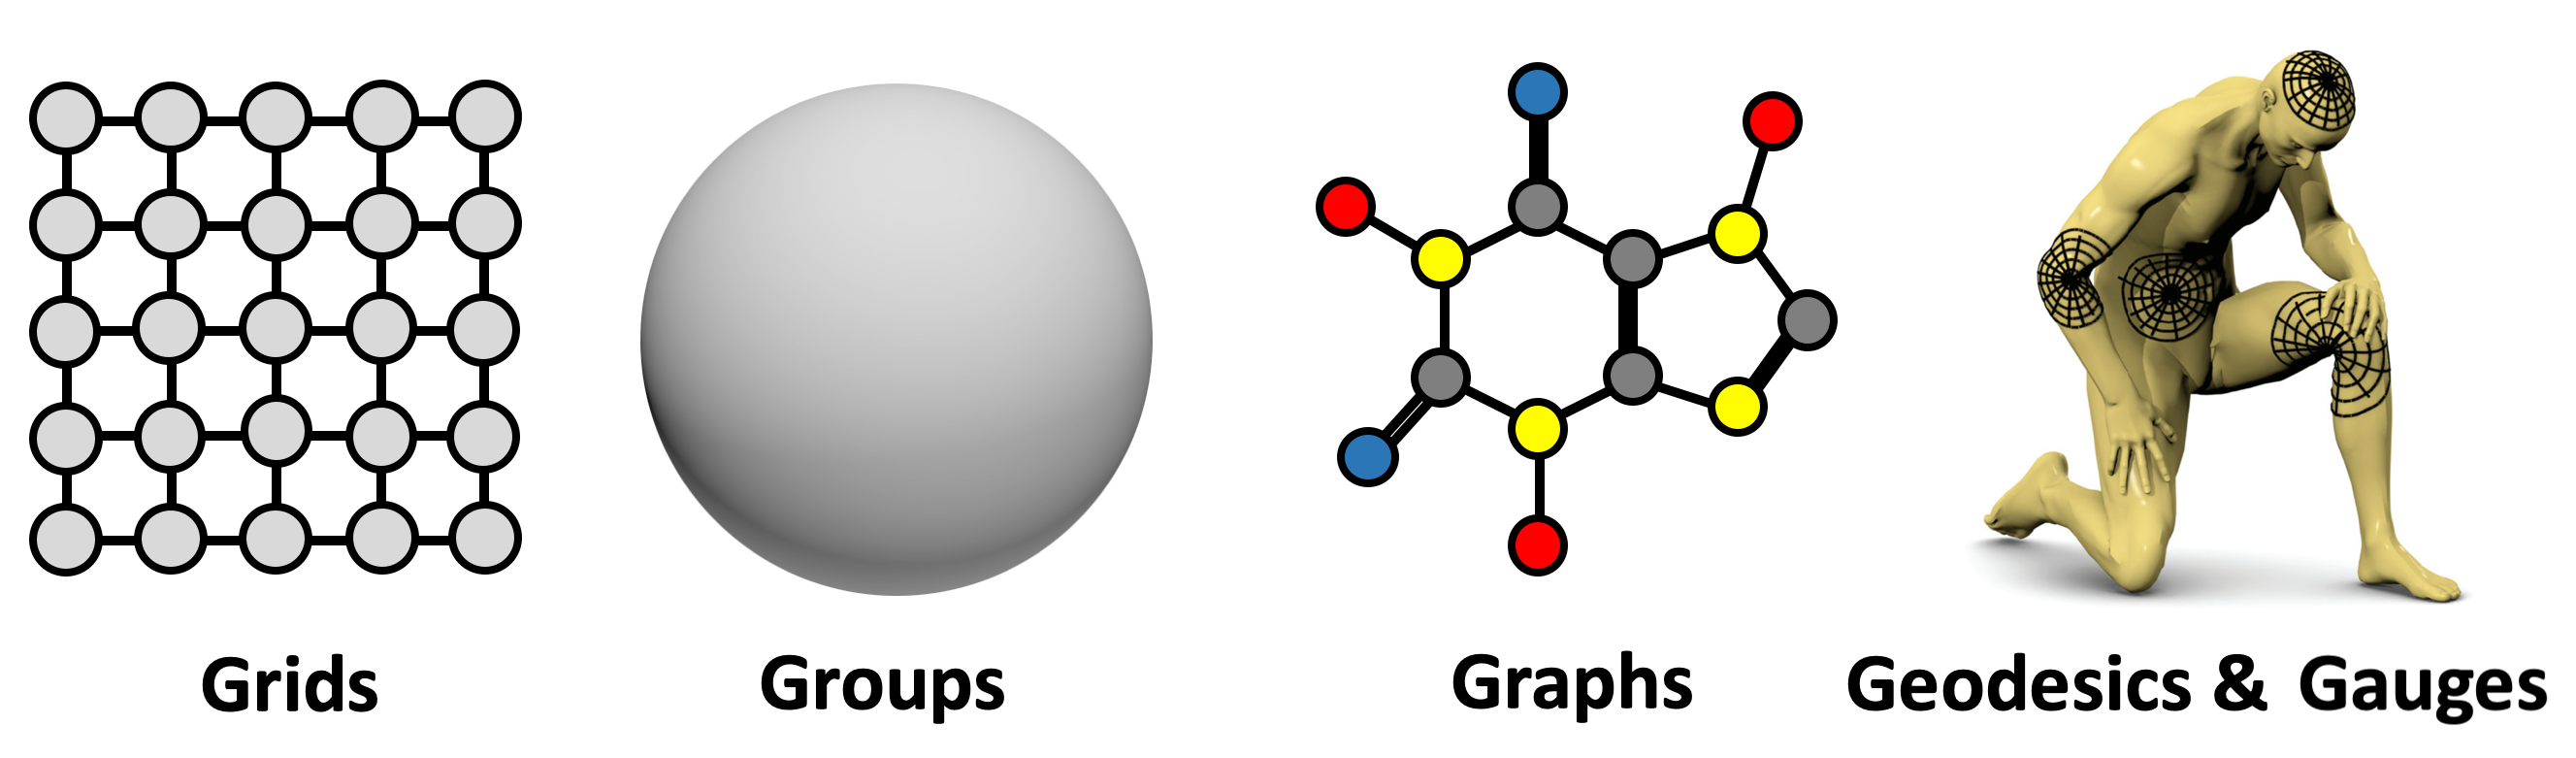
\includegraphics[width=1\textwidth]{figures/5g.png}
    \caption{The 5G of Geometric Deep Learning: grids, groups \& homogeneous spaces with global symmetry, graphs, geodesics \& metrics on manifolds, and gauges (frames for tangent or feature spaces). }
    \label{fig:4g}
\end{figure}





\subsection{Graphs and Sets}\label{sec:proto-graphs}

%\joan{This is a very nice intro. 
%Just one comment: it would be great to use the transition from sets to graphs to reinforce the scale aspect mentioned in the previous sections. Sets cannot be coarsened in non-trivial ways, while graphs can. 

%Another more general aspect that we need to nail in this section that clearly separates the graph treatment from, say the grid treatment: the domain varies with the input and thus becomes `part' of the input. I think again the transition from set to graph is useful here. The set is always the same geometric object modulo the change in size. The graph provides a new input to the system (as you say, via et its adjacency). 
%}





%\michael{\bf [MB: I took the liberty to rewrite this section making it less detailed and more `conversational' like the style of the previous sections in the Introduction chapter, anticipating that Chapter on graphs to be more rigorous.]}


%\joan{Joan: 
% Great detail and everything important seems to be here already. Two remarks:
% \begin{itemize}
%     \item I would frontload the section a bit more, explaining that we will first describe the domain, and then explain how the geometric priors and the blueprint are expressed.
%     \item Currently, this section re-derives the definitions of invariance/equivariance described previously, as well as the blueprint. I think it can be made shorter and more coherent to simply describe the two forms of group representation arising here (one for sets, and the other for graphs, where adjacency is also present), as well as the metric induced in the graph that is used to define local operators. 
%     \item In other words, I think these sections should derive the class of local linear equivariants for each symmetry group under consideration. In this section of sets and graphs, we should explain the two classes that arise (cf Maron et al.). 
%     \item The notation needs to be unified with the previous sections. 
%     
% \end{itemize}
%}

%\michael{MB: Agree in principle but we should not fall into the Bourbaki extreme. I suggest keep domain-specific notation to use familiar concepts and relate them to blueprint on the high level rather than in detail.

%I suggest to remove reference to particular models and talk about general concepts here. 
%}

In multiple branches of science, from sociology to particle physics, graphs are used as models of systems of relations and interactions. From our perspective, graphs give rise to a very basic type of invariance modelled by the group of permutations. 
Furthermore, other objects of interest to us, such as grids and sets, can be obtained as a particular case of graphs.  
%
%since graphs exhibit less restrictive geometries and invariances, they invite for the most flexible class of architectures---the \emph{Graph Neural Networks} (GNN). As we will see, all of the neural architectures we will study in this book can be understood as a special case of the GNN, with injected additional geometric constraints and invariances.


%the {\em symmetric group}), a . 


A {\em graph} $\gG = (\gV, \gE)$ is a collection of {\em nodes}\marginnote{Depending on the application field, nodes may also be called \emph{vertices}, and edges are often referred to as \emph{links} or \emph{relations}. We will use these terms interchangeably.} $\gV$  and {\em edges} $\gE \subseteq \gV\times \gV$ between pairs of nodes. For the purpose of the following discussion, we will further assume the nodes to be endowed with $s$-dimensional {\em node features}, 
denoted by $\mathbf{x}_u$ for all $u \in \gV$. 
%
Social networks are perhaps among the most commonly studied examples of graphs, where nodes represent users, edges correspond to friendship relations between them, and node features model user properties such as age, profile picture, etc. It is also often possible to endow the edges, or entire graphs, with features;\marginnote{
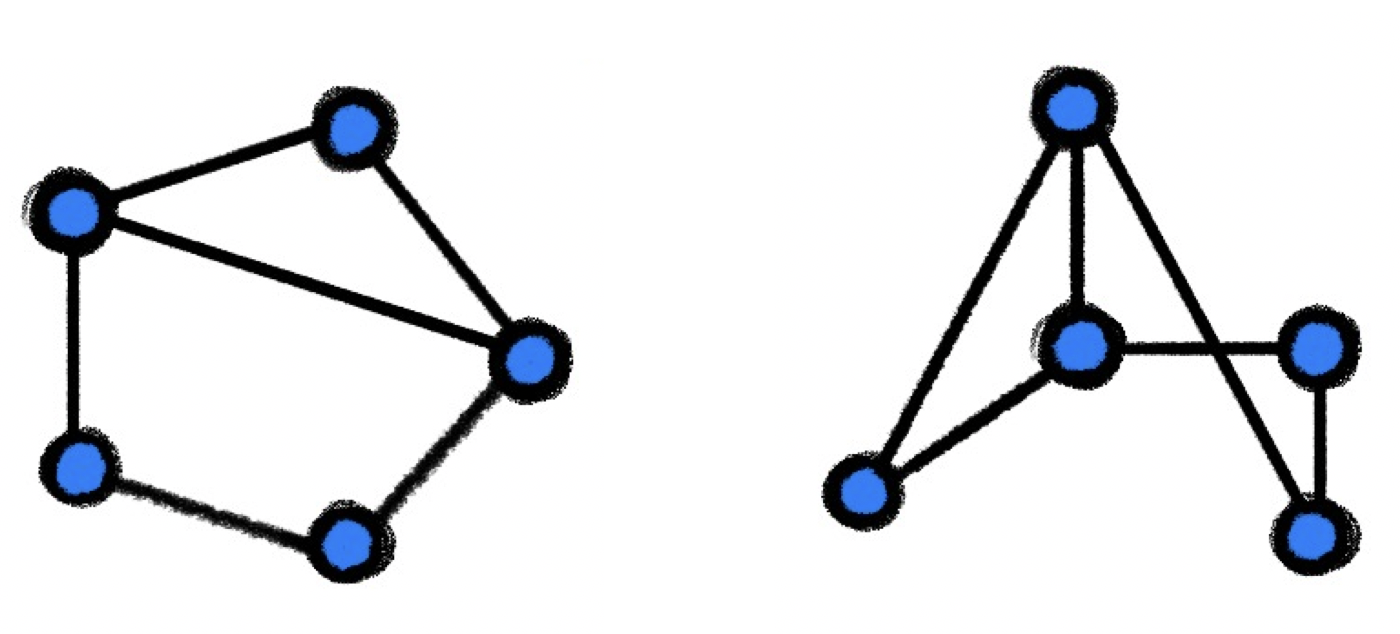
\includegraphics[width=0.8\linewidth]{figures/mn_isomorphic.png}
{\em Isomorphism} is an edge-preserving bijection between two graphs. Two isomorphic graphs shown here are identical up to reordering of their nodes. 
} but as this does not alter the main findings of this section, we will defer discussing it to future work.


The key structural property of graphs is that the nodes in $\gV$ are usually not assumed to be provided in any particular order, and thus any operations performed on graphs should not depend on the ordering of nodes. The desirable property  that functions acting on graphs should satisfy is thus {\em permutation invariance}, and it implies that for any two \emph{isomorphic} graphs,  the outcomes of these functions are identical. 
%
%
%This is clearly a 
We can see this as a 
particular setting of our blueprint, where the domain $\Omega = \mathcal{G}$ and the space $\mathcal{X}(\mathcal{G},\mathbb{R}^d)$ is that of $d$-dimensional node-wise signals. 
%
The symmetry we consider is given by the \emph{permutation group} $\mathfrak{G} = \Sigma_n$, whose elements are all the possible orderings of the set of node indices $\{1,\hdots, n\}$. 

%\michael{Harmonize notation: do we use $s$ or $d$ for dimension of features? } \joan{I am making a pass, using $s$ for feature dimension}\michael{we always used $d$, changing}

%In the language of the previous sections:\marginnote{However, we will almost always omit such notation for graphs, as they are assumed to be \emph{discrete} collections of nodes; hence, the language of linear algebra will admit higher notational simplicity.} for graphs we consider the input space to be defined on the domain  $\Omega = \mathcal{V}$, with the input space $\mathcal{X}(\mathcal{G}) = \{x : \mathcal{V}\rightarrow\mathbb{R}^s\}$ consisting of functions that attach node feature vectors to every node; $x(v) = \vec{x}_v$.
%\joan{Notation-wise: align with previous section $\Omega$ for domain, $\gX$ for signals over the domain} \michael{We use $x$ for signals, but $\Omega$ must be specific. }



%
%Accordingly, we focus on the permutation group actions $\frak{g}\in\frak{G}$ that permute the node ordering by applying such a matrix: $\frak{g}.{\bf X} = {\bf P}{\bf X}$. %


%$$ (where $n$ is the number of nodes).

%\begin{equation}
%    {\bf P}_{(2, 4, 1, 3)}{\bf X} =
%    \left[
%    \begin{array}{cccc}
%        0 & 1 & 0 & 0\\
%        0 & 0 & 0 & 1\\
%        1 & 0 & 0 & 0\\
%        0 & 0 & 1 & 0
%    \end{array}\right]\left[
%  \begin{array}{ccc}
%    \horzbar & \mathbf{x}_1 & \horzbar \\
%    \horzbar & \mathbf{x}_2 & \horzbar \\
%      \horzbar        &   \mathbf{x}_3  &    \horzbar       \\
%    \horzbar & \mathbf{x}_4 & \horzbar
%  \end{array}\right] = \left[\begin{array}{ccc}
%   \horzbar & \mathbf{x}_2 & \horzbar \\
%    \horzbar & \mathbf{x}_4 & \horzbar \\
 %     \horzbar        &   \mathbf{x}_1  &    \horzbar       \\
%    \horzbar & \mathbf{x}_3 & \horzbar
%  \end{array}\right]
%\end{equation}




%The first kind of object we will be studying is that of the \emph{graph}, which corresponds to the mother of all finite symmetry groups: the group of permutations. For the purposes of this chapter, we will define graphs as $G=(V, E)$, where $V$ is the set of \emph{nodes} and $E\subseteq V\times V$ is a set of \emph{edges} between pairs of nodes. For a commonly-studied example, social networks can be readily represented as graphs where nodes correspond to users, and edges correspond to the friendship links between them. 

%For now, we will assume that the graph's nodes are endowed with \emph{node features}, represented by $\mathcal{X} = \left\{\mathbf{x}_1, \mathbf{x}_2, \dots, \mathbf{x}_{|V|}\right\}$, where $\mathbf{x}_i\in\mathbb{R}^k$ are the features of node $i\in V$. In the social network analogy, these features could correspond to (some encoding of) the user's biography, interests or profile picture. Additional featurizations are possible, e.g. having features on the edges or entire graphs, but we will omit them for simplicity for now. 

%Compared with the subsequent objects, graphs exhibit less restrictive geometries and invariances, and hence invite for the most flexible class of architectures---the \emph{Graph Neural Networks} (GNN). Indeed, all of the neural architectures we will study can be understood as a special case of the GNN, with injected additional geometric constraints and invariances.

%The key structural property of graphs is that the nodes in $V$ are usually not assumed to be provided in any particular order, and thus any operations performed on graphs should not depend on the ordering of nodes. This desirable property that operations should satisfy is {\em permutation invariance}, and it implies that for any two \emph{isomorphic} graphs,\footnote{Isomorphism is an edge-preserving bijection between two graphs. Two isomorphic graphs are identical up to reordering of their nodes. } the outcomes of these operations are identical. 


Let us first illustrate the concept of permutation invariance on \emph{sets}, a special case of graphs without edges (i.e., $\gE=\emptyset$). 
%
By stacking the node features as rows of the $n\times d$ matrix
 $\mathbf{X} = (\mathbf{x}_1, \hdots, \mathbf{x}_n)^\top$, we do effectively specify an ordering of the nodes. 
 %
The action of the permutation $\mathfrak{g}\in\Sigma_n$ on  the set of nodes amounts to the reordering of the rows of $\mathbf{X}$, which can be represented as an $n\times n$ {\em permutation matrix} $\rho(\mathfrak{g}) = \mathbf{P}$,\marginnote{There are exactly $n!$ such permutations, so $\Sigma_n$ is, even for modest $n$, a very large group. } where each row and column contains exactly one $1$ and all the other entries are zeros. 



%  We may obtain a different ordering by applying an appropriate permutation matrix  $\mathbf{P}$,\marginnote{There are exactly $n!$ such permutations. } where each row and column contains exactly one $1$ and all the other entries are zeros. Accordingly, we focus on the permutation group actions $\frak{g}\in\frak{G}$ that permute the node ordering by applying such a matrix: $\frak{g}.{\bf X} = {\bf P}{\bf X}$. %
 
 %\begin{equation}
 %    a(\vec{x}, \vec{y}) = \left<\vec{W}\vec{x}, \vec{U}\vec{y}\right> \qquad a(\vec{x}, \vec{y}) = \vec{a}^\top({\bf Wx} + {\bf Uy})
 %\end{equation}
 
 %\begin{align*}
 %    {\bf x}^\top{\bf L}{\bf x} &= \frac{1}{2}\sum_{u\in\mathcal{V}}\sum_{v\in\mathcal{V}} a_{uv}(x_u - x_v)^2\\ &= \sum_{(u, v)\in\mathcal{E}} (x_u - x_v)^2
 %\end{align*}

 
 %, ${\bf P}\in\mathbb{R}^{|V|\times|V|}$, to ${\bf X}$. 
 


%Let ${\bf X}\in\mathbb{R}^{|V|\times k}$ be a \emph{node feature matrix} which is obtained by stacking $\mathbf{x}_i$ in a particular order. This effectively specifies one \emph{ordering} of this set of node features; we may obtain any different order by applying an appropriate permutation matrix, ${\bf P}\in\mathbb{R}^{|V|\times|V|}$, to ${\bf X}$. 
A function $f$ operating on this set is then said to be \emph{permutation invariant} if, for any such permutation matrix ${\bf P}$, it holds that $f({\bf P}{\bf X}) = f({\bf X})$. One simple such function is 
%, exploited by the Deep Sets model \citep{zaheer2017deep}, is
\begin{equation}
\label{eq:basicinv}
    f({\bf X}) = \phi\left(\sum_{u\in \gV} \psi\left(\mathbf{ x}_u\right)\right)~,
\end{equation}
where the function $\psi$ is independently applied to every node's features, and $\phi$ is applied on its \emph{sum-aggregated} outputs: as sum is independent of the order in which its inputs are provided, such a function is  invariant with respect to the permutation of the node set, and is hence guaranteed to always return the same output, no matter how the nodes are permuted.

%\michael{Notation: should we use $\mathbf{f}(\mathbf{X})$ since the output can be a vector?}
%\petar{I would tend to stick with the $f$ notation}

 
%node features in $\mathcal{X}$ are permuted.



Functions like the above provide a `global' graph-wise output, but very often, we will be interested in functions that act `locally', in a node-wise manner. 
%return more fine-grained information. 
For example, we may want to apply some function to \emph{update} the features in every node, obtaining the set of \emph{latent} node features. 
%, $\mathbf{h}_1, \hdots, \mathbf{h}_n$. 
%$\mathcal{H}=\left\{\mathbf{h}_1, \mathbf{h}_2, \dots, \mathbf{h}_{|V|}\right\}$.
%
%Strictly speaking, 
If we stack these latent features into a matrix $\mathbf{H} = \mathbf{F}({\bf X})$\marginnote{We use the bold notation  for our function $\mathbf{F}(\mathbf{X})$ to emphasise it outputs node-wise vector features and is hence a matrix-valued function.} is no longer permutation invariant: the order of the rows of ${\bf H}$ should be \emph{tied} to the order of the rows of ${\bf X}$, so that we know which output node feature corresponds to which input node. We need instead  a more fine-grained notion of {\em permutation equivariance}, stating that, once we ``commit'' to a permutation of inputs, it consistently permutes the resulting objects. 
%
Formally, $\mathbf{F}(\mathbf{X})$ is a \emph{permutation equivariant} function if, for any permutation matrix ${\bf P}$, it holds that $\mathbf{F}({\bf P}{\bf X}) = {\bf P}\mathbf{F}({\bf X})$. A shared node-wise linear transform 
\begin{equation}
    \mathbf{F}_{\mathbf\Theta}({\bf X}) = {\bf X}{\mathbf \Theta}
    %\qquad \text{, i.e.,} \qquad {\vec h}_i = {\mathbf\Theta}^T\mathbf{x}_i
\end{equation}
specified by a weight matrix $\mathbf\Theta\in\mathbb{R}^{d\times d'}$, is one possible construction of such a permutation equivariant function, producing in our example 
latent features of the form 
$\mathbf{h}_u = \boldsymbol{\Theta}^\top\mathbf{x}_u$.
%\joan{This is very clear and nicely explained, but it is a particular case of the group equivariance discussion from previous section. I would add a pointer at the beginning or the end of this paragraph to tie things together. Upps just saw the following paragraph, nevermind. }

%\michael{Notation: do we use $h$ or $y$ for output?}
%\petar{$h$ for what comes out of an equivariant layer; the assumption is that we can stack more than one, or even attach invariant tail, to get a desirable $y$ (which should maybe be reserved for downstream task outputs?).}


%In fact, the construction from Equation (\ref{eq:basicinv}) arises naturally from the GDL blueprint. 
This construction arises naturally from our Geometric Deep Learning blueprint. 
We can first attempt to characterise {\em linear equivariants} (functions of the form $\mathbf{F} {\bf P X} = \bf{P} \mathbf{FX}$), for which it is easy to verify 
that any such map can be written as a linear combination of two \emph{generators}, the identity $\mathbf{F}_1 \mathbf{X} = {\bf X}$ and the average ${\mathbf{F}_2 \mathbf{X}}= \frac{1}{n}\boldsymbol{1}\boldsymbol{1}^\top \mathbf{X} = \frac{1}{n} \sum_{u=1}^n {\bf x}_u$. As will be described in Section \ref{sec:deepset}, the popular Deep Sets \citep{zaheer2017deep} architecture follows precisely this blueprint.
%\joan{Remark to avoid confusion that $\mathbf{X}$ here should be understood as a vector, not a matrix}


% TODO: explain relation to representations & equivariance as explained in previous section.
% Invariant features correspond to a trivial representation
% Node features correspond to rho(P) = P
% Edge features / adjacency matrix corresponds to rho(P) = P tensor P.


We can now generalise the notions of permutation invariance and equivariance from sets to graphs. 
%
In the generic setting $\gE\neq\emptyset$, the graph connectivity can be represented by the $n\times n$ {\em adjacency matrix} $\mathbf{A}$,\marginnote{When the graph is {\em undirected}, i.e. $(u,v) \in \gE$ iff $(v,u) \in \gE$, the adjacency matrix is {\em symmetric}, $\mathbf{A}= \mathbf{A}^\top$. } defined as  
\begin{equation}
    a_{uv} = \begin{cases}
    1 & (u, v)\in \gE\\
    0 & \text{otherwise}.
    \end{cases}
\end{equation}
%
Note that now the adjacency and feature matrices $\mathbf{A}$ and $\mathbf{X}$ are ``synchronised'', in the sense that $a_{uv}$ specifies the adjacency information between the nodes described by the $u$th and $v$th rows of $\mathbf{X}$. Therefore, applying a permutation matrix $\mathbf{P}$ to the node features $\mathbf{X}$ automatically implies applying it to $\mathbf{A}$'s rows and columns, $\mathbf{P}\mathbf{A}\mathbf{P}^\top$. \marginnote{$\mathbf{P}\mathbf{A}\mathbf{P}^\top$ is the representation of $\Sigma_n$ acting on matrices. }
%
%
We say that (a graph-wise function) $f$ is \emph{permutation invariant} if  
\begin{equation}
f({\bf PX}, {\bf PAP}^\top) = f({\bf X}, {\bf A})\marginnote{As a way to emphasise the fact that our functions operating over graphs now need to take into account the adjacency information, we use the notation $f({\bf X}, {\bf A})$.}
\end{equation}
and (a node-wise function) $\mathbf{F}$ is \emph{permutation equivariant} if 
\begin{equation}
\label{eq:permequivgraph}
\mathbf{F}({\bf PX}, {\bf PAP}^\top) = {\bf P}\mathbf{F}({\bf X}, {\bf A})
\end{equation}
for any permutation matrix  ${\bf P}$.
%
%
%\taco{Taco: should we relate this to the blueprint? We can mention here that $PX$ and $PAP^T$ are examples of representations of the permutation group. We can then go on to say that the graph structure tells us which nodes are close in a certain sense, and that most graph nets exploit this, leading into the next paragraph.}\michael{I do say above that $\rho(\fg)=P$}
%
%Armed with the concepts of permutation invariance and equivariance, we can consider a generic graph connectivity setup, where $E\neq\emptyset$. One typical way to represent this adjacency information in a compact form is the \emph{adjacency matrix}, ${\bf A}\in\mathbb{R}^{|V|\times|V|}$, which is in the simplest case (of an unweighted and undirected graph), a binary and symmetric matrix; that is:
%\begin{equation}
%    {\bf A}_{ij} = {\bf A}_{ji} = \begin{cases}
%    1 & (i, j)\in E\\
%    0 & \text{otherwise}
%    \end{cases}
%\end{equation}
%
%
%We can now generalise the notions of permutation invariance and equivariance from sets to graphs. We note that the order of the rows and columns in ${\bf A}$ is constrained to respect the order of the rows of ${\bf X}$---that is, ${\bf A}_{ij}$ specifies the adjacency information between the nodes described by the $i$-th and $j$-th row of ${\bf X}$. Then, applying a permutation matrix ${\bf P}$ to the nodes in ${\bf X}$ automatically implies applying it to ${\bf A}$'s rows and columns, yielding ${\bf P}{\bf A}{\bf P}^T$. 


%Following again the Geometric Deep Learning blueprint, 
Here again, we can first characterise linear equivariant functions.\marginnote{This corresponds to the {\em Bell number} $B_4$, which counts the number of ways to partition a set of $4$ elements, in this case given by the 4-indices $(u,v), (u',v')$ indexing a linear map acting on the adjacency matrix.  %\cite{maron2018invariant}.
}  
As observed by \cite{maron2018invariant}, any linear $\mathbf{F}$ satisfying equation (\ref{eq:permequivgraph}) can be expressed as a linear combination 
of fifteen linear generators; remarkably, this family of generators is {\em independent of} $n$. 
%
%
%
Amongst these generators, our blueprint specifically advocates for those that are also {\em local}, i.e., whereby  
the output on node $u$ directly depends on its neighbouring nodes in the graph. We can formalise this constraint explicitly in our model construction, by defining what it means for a node to be neighbouring another.



A (undirected) {\em neighbourhood} of node $u$, sometimes also called {\em 1-hop},  is defined as \marginnote{
%Our definition of neighbourhood does not account for directed edges. 
Often, the node $u$ itself is included in its own neighbourhood.}
\begin{equation}
    \mathcal{N}_u = \{ v : (u,v) \in \gE \,\mathrm{or}\, (v,u) \in \gE \}
    %\left\{j\ |\ i=j\vee {\bf A}_{ij} = 1\right\}
\end{equation}
%
and the {\em neighbourhood features} as the multiset 
%
\begin{equation}
    \mathbf{X}_{\mathcal{N}_u} = \ldblbrace \mathbf{x}_v : v\in\mathcal{N}_u \rdblbrace.
\marginnote{A {\em multiset}, denoted $\ldblbrace \, \dots \, \rdblbrace$, is a set where the same element can appear more than once. This is the case here because the features of different nodes can be equal.}
\end{equation}
%%
Operating on 1-hop neighbourhoods aligns well with the \emph{locality} aspect of our blueprint: namely, defining our metric over graphs as the \emph{shortest path distance} between nodes using edges in $\mathcal{E}$.% \michael{I suggest we get rid of this, since we never talked about metrics in a rigorous way. } \petar{There seems to still be a discussion of a metric when defining locality in the blueprint---this is what I was referring to. I think it's fine as-is, but wouldn't mind removing it.} \joan{I think mentioning it qualitatively like this is fine, it conveys an important message}
%Processing 1-hop neighbourhoods over graphs exactly corresponds with defining our metric over graphs, $g$, as the \emph{shortest path distance} between nodes using edges in $\mathcal{E}$, and setting $\delta = 1$.

%This also closely aligns with the \emph{locality} condition of the main building block of our geometric deep learning blueprint. Processing 1-hop neighbourhoods over graphs exactly corresponds with defining our metric over graphs, $g$, as the \emph{shortest path distance} between nodes using edges in $\mathcal{E}$, and setting $\delta = 1$.

%
The GDL blueprint thus yields a general recipe for constructing permutation equivariant functions on graphs, by specifying a \emph{local} function $\phi$ that operates over the features of a node and its neighbourhood, $\phi(\mathbf{x}_u, \mathbf{X}_{\mathcal{N}_u})$. Then, a permutation equivariant function $\mathbf{F}$ can be constructed by applying $\phi$ to every node's neighbourhood in isolation (see Figure \ref{fig:gc_gdl}):
\begin{equation}
    \mathbf{F}({\bf X}, {\bf A}) =
\left[
  \begin{array}{ccc}
    \horzbar & \phi(\mathbf{x}_1, \mathbf{X}_{\mathcal{N}_1}) & \horzbar \\
    \horzbar & \phi(\mathbf{x}_2, \mathbf{X}_{\mathcal{N}_2}) & \horzbar \\
             & \vdots    &          \\
    \horzbar & \phi(\mathbf{x}_n, \mathbf{X}_{\mathcal{N}_n}) & \horzbar
  \end{array}
\right]
\label{eq:graph_equivariant}
\end{equation}
As $\mathbf{F}$ is constructed by applying a shared function $\phi$ to each node locally, its permutation equivariance rests on $\phi$'s output being independent on the ordering of the nodes in $\mathcal{N}_u$. Thus, if $\phi$ is built to be permutation invariant, then this property is satisfied.
%
As we will see in future work, the choice of $\phi$ plays a crucial role in the expressive power of such a  scheme. When $\phi$ is injective, it is equivalent to one step of the {\em Weisfeiler-Lehman graph isomorphism test}, a classical algorithm in graph theory providing a necessary condition for two graphs to be isomorphic by an iterative color refinement procedure. 


%\michael{ADD: geometric stability of graph filters}

%We conclude our introduction with a discussion on how to generally construct useful functions over graphs that are permutation equivariant. A function over graphs is likely to be useful if it directly exploits the structure present in ${\bf A}$---that is, if outputs on node $i$ directly depend on its \emph{neighbouring} nodes in the graph (e.g. the non-zero entries of $\mathbf{a}_i$ and $\mathbf{a}_i^T$).

%From this concept, we can define a \emph{neighbourhood} of node $i$ in the graph, commonly denoted as $\mathcal{N}_i$, to include all first-order neighbours of $i$, often including $i$ itself:
%\begin{equation}
%    \mathcal{N}_i = \left\{j\ |\ i=j\vee {\bf A}_{ij} = 1\right\}
%\end{equation}
%Accordingly, we can define the set of \emph{neighbourhood features} of $i$, $\mathbf{X}_{\mathcal{N}_i}\in\mathcal{P}(\mathbb{R}^k)$:
%\begin{equation}
%    \mathbf{X}_{\mathcal{N}_i} = \left\{\mathbf{x}_j\ |\ j\in\mathcal{N}_i\right\}
%\end{equation}
\begin{figure}
    \centering
    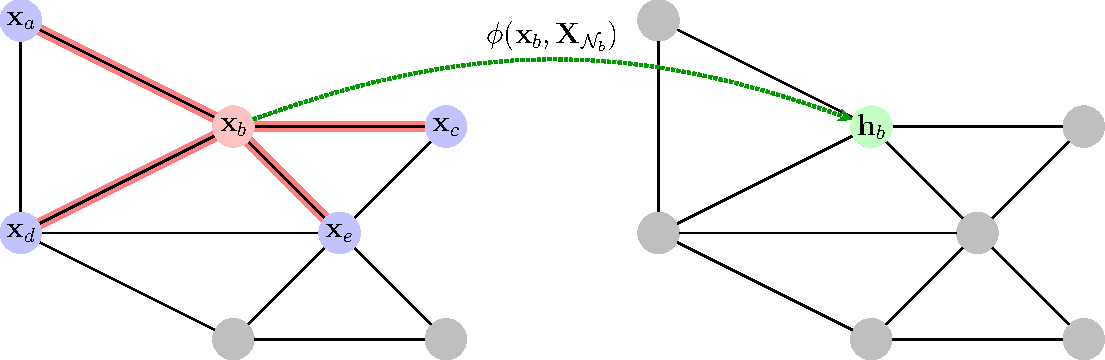
\includegraphics[width=\linewidth]{figures/GC_GDL.pdf}
    \caption{An illustration of constructing permutation-equivariant functions over graphs, by applying a permutation-invariant function $\phi$ to every neighbourhood. In this case, $\phi$ is applied to the features $\mathbf{x}_b$ of node $b$ as well as the multiset  of its neighbourhood features, $\mathbf{X}_{\mathcal{N}_b} = \ldblbrace\mathbf{x}_a, \mathbf{x}_b, \mathbf{x}_c, \mathbf{x}_d, \mathbf{x}_e\rdblbrace$. Applying $\phi$ in this manner to every node's neighbourhood recovers the rows of the resulting matrix of latents features $\mathbf{H}=\mathbf{F}(\mathbf{X}, \mathbf{A})$.}
    \label{fig:gc_gdl}
\end{figure}%
%\michael{\bf [MB: shall we use the notation of multisets here?]}


%The general concept of constructing {\em permutation equivariant} functions operating over graphs as shared {\em permutation invariant} functions operating over local neighbourhoods appears to be very powerful and underlies the design of most Graph Neural Networks. Under various guises, this local function $g$ can be referred to as ``diffusion'', ``propagation'', or ``message passing''. 
%
%If we are interested in a graph-level output, a common recipe is to construct the latent node features using a {\em permutation equivariant} function $f$, followed by a {\em permutation invariant} function $h$ over the entries of $f({\bf X}, {\bf A})$ to obtain an ordering-independent output. In this context, the function $h$ is often referred to as ``readout'' or ``global pooling''.

%Motivation: examples from 
%- Images, Text, Speech. 
%- Social Networks
%- Physical Sciences
%- Chemistry and medicine
%- 3D Computer vision and Graphics


%Finally, 
It is also worth noticing that the difference between functions defined on sets and more general graphs in this example is that in the latter case we need to explicitly account for the structure of the domain. 
%
As a consequence, graphs stand apart in the sense that the domain becomes {\em part of the input} in machine learning problems, whereas when dealing with sets and grids (both particular cases of graphs) we can specify only the features and assume the domain to be {\em fixed}. 
%
This distinction will be a recurring motif in our discussion. 
%
As a result, the notion of geometric stability (invariance to domain deformation) is crucial in most problems of learning on graphs. It straightforwardly follows from our construction that permutation invariant and equivariant functions produce identical outputs on isomorphic (topologically-equivalent) graphs. These results can be generalised to approximately isomorphic graphs, and several results on stability under graph perturbations exist  \citep{levie2018cayleynets}.  We will return to this important point in our discussion on manifolds, which we will use as an vehicle to study such invariance in further detail. 


Second, due to their additional structure, graphs and grids, unlike sets, can be coarsened in a non-trivial way\marginnote{More precisely, we cannot define a non-trivial coarsening assuming set structure alone. There exist established approaches that infer topological structure from unordered sets, and those can admit non-trivial coarsening.}, giving rise to a variety of pooling operations. 
%These will also be covered within Chapter \ref{ch:graphs}. 
%
%Finally, 



\subsection{Grids and Euclidean spaces} 
\label{sec:grids_euclidean}

%\joan{Joan: Good section; perhaps we could shrink a bit by removing the repetitive parts between blueprint, discrete and then continuous case. Also further highlight the fundamental differences between grids and graphs in terms of group representation (permutation group vs translation group, one-parameter group in one case), and geometry (homogeneous vs non-homogeneous): consequences in terms of global orientation, etc. 
%}
%\michael{This more naturally comes after the Groups section, was a natural transition to manifolds which are non-homogeneous}

%images, CNNs, RNNs

The second type of objects we consider are grids. 
%
It is fair to say that the impact of deep learning was particularly dramatic in computer vision,  natural language processing, and speech recognition. These applications all share a %an essential 
geometric common denominator: an underlying grid structure. 
%translation invariance/equivariance, alongside scale separation. 
%
As already mentioned, grids are a particular case of graphs with special adjacency. However, since the order of nodes in a grid is fixed, machine learning models for signals defined on grids are no longer required to account for permutation invariance, and have a stronger geometric prior: translation invariance. 
%can be designed to leverage the translation invariance prior. 

%This gives rise to powerful and efficient deep learning architectures---{\em Convolutional Neural Networks} (CNNs). 



\paragraph{Circulant matrices and Convolutions}
Let us dwell on this point in more detail. 
Assuming for simplicity periodic boundary conditions, we can think of a one-dimensional grid as a {\em ring graph}\marginnote{
    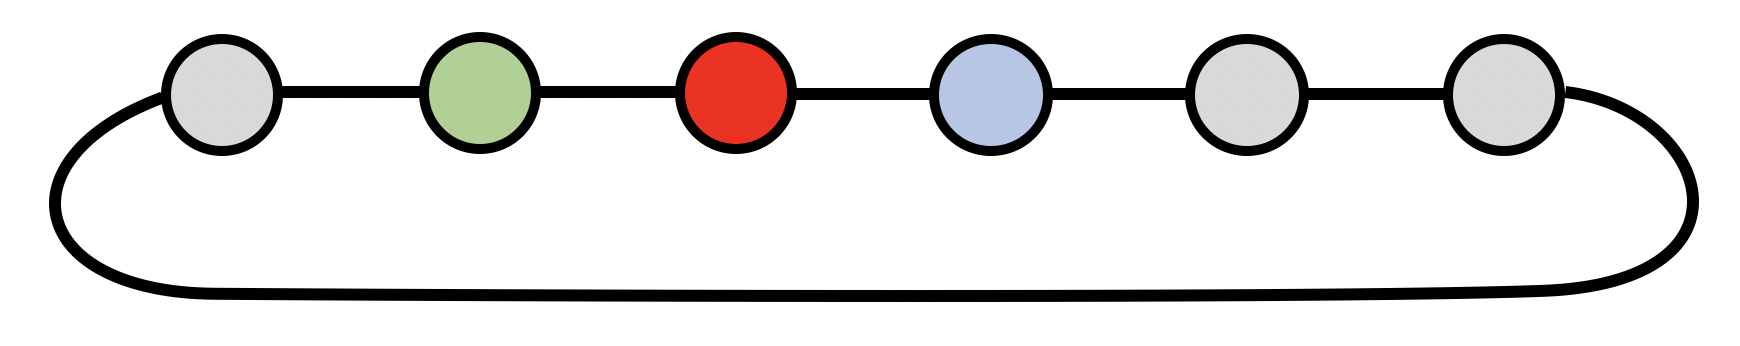
\includegraphics[width=0.9\linewidth]{figures/grid.png}
} with nodes indexed by $0, 1,\hdots, n-1$ modulo $n$ (which we will omit for notation brevity) and
the adjacency matrix with elements $a_{u,u+1 \, \mathrm{mod} \, n} = 1$ and zero otherwise. There are two main differences from the general graph case we have discussed before. 
%
First, each node $u$ has identical connectivity, to its neighbours $u-1$ and $u+1$, and thus structure-wise indistinguishable from the others. 
%in terms of group theory, we say that the grid is a homogeneous space. 
\marginnote{As we will see later, this makes the grid a homogeneous space.
  %  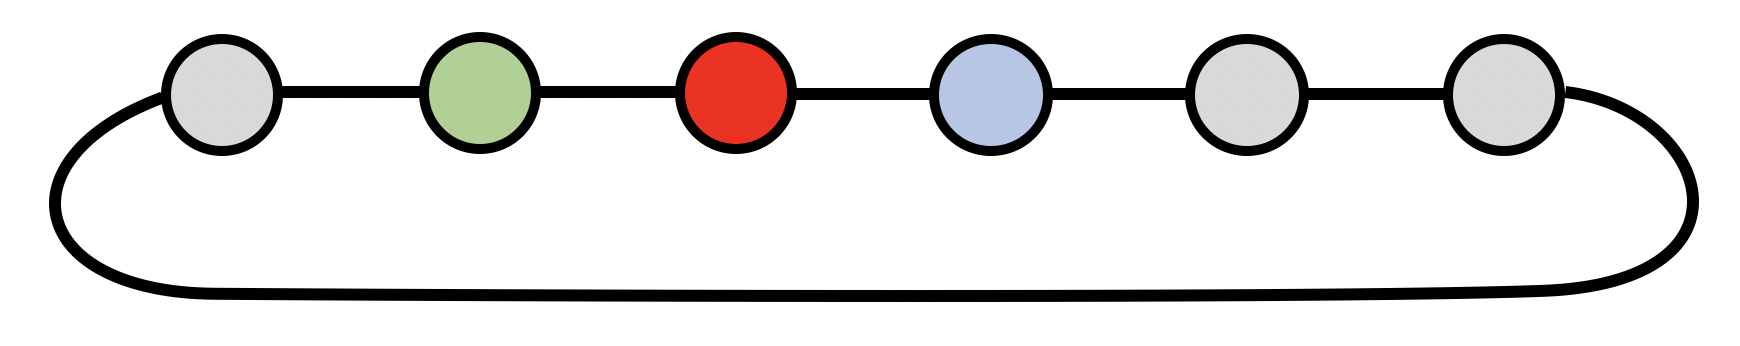
\includegraphics[width=1\linewidth]{figures/grid.png}
}
%
Second and more importantly, since the nodes of the grid have a fixed ordering, we also have a fixed ordering of the {\em neighbours:} we can call $u-1$ the `left neighbour' and $u+1 $ the `right neighbour'.
%
If we use our previous recipe for designing a equivariant function $\mathbf{F}$ using a local aggregation function $\phi$, we now have $\mathbf{f}(\mathbf{x}_u) = \phi(\mathbf{x}_{u-1}, \mathbf{x}_{u}, \mathbf{x}_{u+1})$ at every node of the grid: $\phi$ does not need to be permutation invariant anymore.  
%
%
For a particular choice of a linear transformation $\phi(\mathbf{x}_{u-1}, \mathbf{x}_{u}, \mathbf{x}_{u+1}) = \theta_{-1}\mathbf{x}_{u-1} + \theta_0 \mathbf{x}_{u} + \theta_1 \mathbf{x}_{u+1}$, we can write $\vec{F}(\mathbf{X})$ as a matrix product, 
$$
\vec{F}(\mathbf{X}) = 
\left[
\begin{array}{ccccc}
\theta_0 & \theta_1  & & & \theta_{-1}\\
 \theta_{-1} & \theta_0 & \theta_1 & & \\
&  \ddots & \ddots & \ddots & \\
 &  & \theta_{-1} & \theta_0 & \theta_1\\
\theta_1 &  &  & \theta_{-1} & \theta_0

 \end{array}
  \right]
  %
\left[  
    \begin{array}{ccc}
    \horzbar & \mathbf{x}_0 & \horzbar \\
    \horzbar & \mathbf{x}_1 & \horzbar \\
             & \vdots    &          \\
    \horzbar & \mathbf{x}_{n-2} & \horzbar  \\           
    \horzbar & \mathbf{x}_{n-1} & \horzbar
  \end{array}
   \right]
$$
%
Note this very special multi-diagonal structure with one element repeated along each diagonal, sometimes referred to as ``weight sharing'' in the machine learning literature. 
%
%In machine learning literature, it is sometimes referred to as %``weight sharing'', a prominent feature of CNNs where the same %weights are applied at different positions in an image. 

%\michael{Notation: we denoted filters by $\theta$}

More generally, given a vector $\boldsymbol{\theta} = (\theta_0, \hdots, \theta_{n-1})$, a {\em circulant matrix} 
$\mathbf{C}(\boldsymbol{\theta}) = (\theta_{u-v \, \mathrm{mod} \, n})$ is obtained by appending circularly shifted versions of the vector $\boldsymbol{\theta}$.  
%
Circulant matrices are synonymous with discrete convolutions, \marginnote{Because of the periodic boundary conditions, it is a {\em circular} or {\em cyclic convolution}. In signal processing, $\boldsymbol{\theta}$ is often referred to as the ``filter,'' and in CNNs, its coefficients are learnable. } 
%\taco{TODO: change this equation to a cross-correlation, and add a note saying that technically this is called a cc but we'll call it a conv.}
$$
(\mathbf{x} \star \boldsymbol{\theta})_u = \sum_{v=0}^{n-1}  x_{v \, \mathrm{mod}\, n} \,\, \theta_{u-v \, \mathrm{mod}\, n}
$$
%
as one has $\mathbf{C}(\boldsymbol{\theta})\mathbf{x} = \mathbf{x} \star \boldsymbol{\theta}$. 
%\petar{Should $i$ be replaced with $u$ in the equation above, given our blueprint? I did this in the CNN section.}
%
A particular choice of $\boldsymbol{\theta}=(0,1,0,\hdots, 0)^\top$ yields a special circulant matrix that shifts vectors to the right by one position. This matrix is called the (right) {\em shift} or {\em translation operator}  and denoted by $\mathbf{S}$.\marginnote{The left shift operator is given by $\mathbf{S}^\top$. Obviously, shifting left and then right (or vice versa) does not do anything, which means $\mathbf{S}$ is {\em orthogonal}: $\mathbf{S}^\top \mathbf{S} = \mathbf{S} \mathbf{S}^\top = \mathbf{I}$.} 


%\michael{Notation: Replace $T$ by $S$}


%\michael{Naming: shift vs translation}


Circulant matrices can be characterised by their {\em commutativity} property: the product of circulant matrices is commutative, i.e. 
$\mathbf{C}(\boldsymbol{\theta}) \mathbf{C}(\boldsymbol{\eta}) = \mathbf{C}(\boldsymbol{\eta}) \mathbf{C}(\boldsymbol{\theta})$ for any $\boldsymbol{\theta}$ and $\boldsymbol{\eta}$.
%
Since the shift is a circulant matrix, we get the familiar {\em translation} or {\em shift equivariance} of the convolution operator, 
$$
\mathbf{S} \mathbf{C}(\boldsymbol{\theta}) \mathbf{x} = 
\mathbf{C}(\boldsymbol{\theta}) \mathbf{S} \mathbf{x}.
$$
%
Such commutativity property should not be surprising, since the underlying symmetry group (the translation group) is Abelian. 
Moreover, the opposite direction appears to be true as well, i.e. 
a matrix is circulant iff it commutes with shift.
%
This, in turn, allows us to {\em define} convolution as a translation equivariant linear operation, and is a nice illustration of the power of geometric priors and the overall philosophy of Geometric ML: convolution emerges from the first principle of translational symmetry. 


Note that unlike the situation on sets and graphs, the number of linearly independent shift-equivariant functions (convolutions) \emph{grows} with the size of the domain (since we have one degree of freedom in each diagonal of a circulant matrix). However, the scale separation prior guarantees filters can be {\em local}, resulting in the same $\Theta(1)$-parameter complexity per layer, as we will verify in Section \ref{sec:cnnsec} when discussing the use of these principles in the implementation of Convolutional Neural Network architectures.

%\joan{Link to GDL blueprint: 
%Convolutions also emerge as the essential device to build stable translation invariant representations, by querying the GDL blueprint. 
%Remark that, as opposed to the permutation group in sets and graphs, the number of linearly independent convolution maps \emph{grows} with the size of the domain (since we have one degree of freedom in each diagonal of a circulant matrix). However, the scale separation prior imposes only local filters, resulting in the same $\Theta(1)$-parameter complexity per layer, as we will verify in Section \ref{sec:cnnsec}.  }



\paragraph{Derivation of the discrete Fourier transform}
We have already mentioned the Fourier transform and its connection to convolution: the fact that the Fourier transform diagonalises the convolution operation is an important property used in signal processing to perform convolution in the frequency domain as an element-wise product of the Fourier transforms. 
%
However, textbooks usually only state this fact, rarely explaining {\em where} the Fourier transform comes from and what is so {\em special} about the Fourier basis. 
%
Here we can show it, demonstrating once more how foundational are the basic principles of symmetry. 


For this purpose, recall a fact from linear\marginnote{We must additionally assume distinct eigenvalues, otherwise there might be multiple possible diagonalisations. This assumption is satisfied with our choice of $\mathbf{S}$.}  algebra that (diagonalisable) matrices are {\em joinly diagonalisable} iff they mutually commute. 
%
In other words, there exists a common eigenbasis for all the circulant matrices, in which they differ only by their eigenvalues. 
%
We can therefore pick one circulant matrix and compute its eigenvectors---we are assured that these will be the eigenvectors of all other circulant matrices as well.
%\taco{I think this is true only if all eigenvalues of this matrix are distinct. Take e.g. the identity matrix, which is circulant, and can be (re-)diagonalized by any orthogonal matrix. Using the shift operator is fine in this respect}\michael{The statement here is on the existence of a joint diagonalization. True, some circulant matrices have different bases diagonalizing them, but not all of them will diagonalize other matrices. }
It is convenient to pick the shift operator, for which the eigenvectors happen to be the discrete Fourier basis \marginnote{
$\mathbf{S}$ is orthogonal but non-symmetric, hence, its eigenvectors are orthogonal but the eigenvalues are complex (roots of unity). 
}
$$
\boldsymbol{\varphi}_k = \frac{1}{\sqrt{n}}\left (1, e^{ \frac{2\pi \mi k}{n}}, e^{ \frac{4\pi \mi k}{n} }, \hdots , e^{ \frac{2\pi \mi  (n-1)k}{n} }
\right)^\top, \hspace{5mm} k = 0, 1, \hdots, n-1,  
$$
%
which we can arrange into an $n\times n$ Fourier matrix $\boldsymbol{\Phi} = (\boldsymbol{\varphi}_0, \hdots, \boldsymbol{\varphi}_{n-1})$.
% 
%
Multiplication by $\boldsymbol{\Phi}^*$\marginnote{Note that the eigenvectors are complex, so we need to take complex conjugation when transposing $\boldsymbol{\Phi}$.} 
gives the Discrete Fourier Transform (DFT), and by $\boldsymbol{\Phi}$ the inverse DFT, 
$$
\hat{x}_k = \frac{1}{\sqrt{n}}\sum_{u = 0}^{n-1}x_u e^{-\frac{2\pi \mi k u}{n} } \hspace{15mm}
%
{x}_u = \frac{1}{\sqrt{n}} \sum_{k = 0}^{n-1}\hat{x}_k e^{+\frac{2\pi \mi k u}{n} }.
$$

 
 
Since all circulant matrices are jointly diagonalisable,\marginnote{
Since the Fourier transform is an orthogonal matrix ($\boldsymbol{\Phi}^* \boldsymbol{\Phi} = \mathbf{I}$), geometrically it acts as a change of the system of coordinates that amounts to an $n$-dimensional rotation. In this system of coordinates (``Fourier domain''), the action of a circulant $\mathbf{C}$ matrix becomes element-wise product.
}  
they are also diagonalised by the Fourier transform 
and differ only in their eigenvalues. Since the eigenvalues of the circulant matrix $\mathbf{C}(\boldsymbol{\theta})$ are the Fourier transform of the filter (see e.g. \cite{bamieh2018discovering}), $\hat{\boldsymbol{\theta}} = \boldsymbol{\Phi}^* \boldsymbol{\theta}$, we obtain the Convolution Theorem: 
$$
\mathbf{C}(\boldsymbol{\theta}) \mathbf{x} = \boldsymbol{\Phi}
\left[  
    \begin{array}{ccc}
    \hat{\theta}_0 &  &  \\
    & \ddots & \\
    & & \hat{\theta}_{n-1}
  \end{array}
   \right]\boldsymbol{\Phi}^*\mathbf{x}
   = \boldsymbol{\Phi} (\hat{\boldsymbol{\theta}} \odot \hat{\mathbf{x}} )
$$
%

Because the Fourier matrix $\boldsymbol{\Phi}$ has a special algebraic structure, the products $\boldsymbol{\Phi}^\star \mathbf{x}$ and $\boldsymbol{\Phi} \mathbf{x}$ can be computed with $\mathcal{O}(n \log n)$ complexity using a Fast Fourier Transform (FFT) algorithm. This is one of the reasons why frequency-domain filtering is so popular in signal processing; furthermore, the filter is typically designed directly in the frequency domain, so the Fourier transform $\hat{\boldsymbol{\theta}}$ is never explicitly computed.


Besides the didactic value of the derivation of the Fourier transform
and convolution we have done here, it provides a scheme to generalise these concepts to graphs. Realising that the adjacency matrix of the ring graph is exactly the shift operator, one can can develop the graph Fourier transform and an analogy of the convolution operator by computing the eigenvectors of the adjacency matrix (see e.g. \cite{sandryhaila2013discrete}).
%
Early attempts to develop graph neural networks by analogy to CNNs, sometimes termed `spectral GNNs', exploited this exact blueprint.\marginnote{In graph signal processing, the eigenvectors of the {\em graph Laplacian} are often used as an alternative of the adjacency matrix to construct the graph Fourier transform, see \cite{shuman2013emerging}. On grids, both matrices have joint eigenvectors, but on graphs they results in somewhat different though related constructions.} 
%
We will see in %Chapter~\ref{ch:graphs} 
Sections~\ref{sec:manifolds}--\ref{sec:meshes}
that this analogy has some important limitations. 
%
The first limitation comes from the fact that a grid is fixed, and hence all signals on it can be represented in the same Fourier basis. In contrast, on general graphs, the Fourier basis depends on the structure of the graph. Hence, we cannot directly compare Fourier transforms on two different graphs --- a problem that translated into a lack of generalisation in machine learning problems. 
%
Secondly, multi-dimensional grids, which are constructed as tensor products of one-dimensional grids, retain the underlying structure: the Fourier basis elements and the corresponding frequencies (eigenvalues) can be organised in multiple dimensions. In images, for example, we can naturally talk about horizontal and vertical frequency and filters have a notion of {\em direction}. On graphs, the structure of the Fourier domain is one-dimensional, as we can only organise the Fourier basis functions by the magnitude of the corresponding frequencies. As a result, graph filters are oblivious of direction or {\em isotropic}. 



\paragraph{Derivation of the continuous Fourier transform}
For the sake of completeness, and as a segway for the next discussion, we repeat our analysis in the continuous setting. 
Like in Section~\ref{sec:scale_separation}, consider functions defined on $\Omega = \mathbb{R}$ and the translation operator $(S_v f)(u) = f(u-v)$ shifting $f$ by some position $v$. 
 %
 Applying $S_v$ to the Fourier basis functions $\varphi_\xi(u) = e^{\mi \xi u}$  yields, by associativity of the exponent,  
% \michael{Notation: same $\phi$ used to denote basis functions, filters, and local aggregators}
$$
S_v e^{\mi\xi u} = e^{\mi\xi (u-v)} = e^{-\mi\xi v} e^{\mi\xi u},
$$
i.e., $\varphi{u}_\xi(u)$ is the complex eigenvector of $S_v$ with the complex eigenvalue  $e^{-\mi\xi v} $ -- exactly mirroring the situation we had in the discrete setting. 
Since $S_v$ is a unitary operator (i.e., $\| S_v x \|_p = \| x \|_p$ for any $p$ and $x \in L_p(\R)$), any eigenvalue $\lambda$ must satisfy $|\lambda|=1$, which corresponds precisely to the eigenvalues $e^{-i\xi v}$ found above. 
Moreover, the spectrum of the translation operator is \emph{simple}, meaning that two functions sharing the same eigenvalue must necessarily be collinear. Indeed, suppose that $S_v f = e^{-\mi \xi_0 v} f$ for some $\xi_0$. Taking the Fourier transform in both sides, we obtain 
$$\forall ~\xi~,~e^{-\mi \xi v} \hat{f}(\xi) = e^{-\mi \xi_0 v} \hat{f}(\xi)~,$$
which implies that $\hat{f}(\xi)=0$ for $\xi \neq \xi_0$, thus $f = \alpha \varphi_{\xi_0}$.

For a general linear operator $C$ that is translation equivariant ($S_v C = C S_v$), we have   
$$
S_v C e^{\mi\xi u} = C S_v e^{\mi\xi u} = e^{-\mi\xi v} C e^{\mi\xi u}, 
$$
implying that $C e^{\mi\xi u}$ is also an eigenfunction\marginnote{{\em Eigenfunction} is synonymous with `eigenvector' and is used when referring to eigenvectors of continuous operators.} of $S_v$ with eigenvalue $e^{-\mi\xi v}$, 
from where it follows from the simplicity of spectrum that $C e^{\mi\xi u} = \beta \varphi_{\xi}(u)$; in other words, the Fourier basis is the eigenbasis of all translation equivariant operators.  
%
As a result, $C$ is \emph{diagonal} in the Fourier domain and can be  expressed as $C e^{\mi\xi u} = \hat{p}_{C}(\xi) e^{\mi\xi u}$, where $\hat{p}_{C}(\xi)$ is a {\em transfer function} acting on different frequencies $\xi$.  
%
%
Finally, for an arbitrary function $x(u)$, by linearity, 
%\michael{Notation: use $\lambda$ in place of $\xi$ for frequency?}
%
\begin{eqnarray*}
(C x) (u) &=& C \int_{-\infty}^{+\infty} \hat{x}(\xi) e^{\mi \xi u} \mathrm{d}\xi = \int_{-\infty}^{+\infty} \hat{x}(\xi) \hat{p}_C(\xi) e^{\mi \xi u} \mathrm{d}\xi \\
&=& \int_{-\infty}^{+\infty} p_C(v) x(u-v) \mathrm{d}v~ = (x \star p_C)(u),\marginnote{The spectral characterisation of the translation group is a particular case of a more general result in Functional Analysis, the \emph{Stone's Theorem}, which derives an equivalent characterisation for any one-parameter unitary group.}
\end{eqnarray*}
%
where $p_C(u)$ is the inverse Fourier transform of $\hat{p}_C(\xi)$. It thus follows that every linear translation equivariant operator is a convolution. 
% {\em quod erat demonstrandum}.










%\michael{Multi-dimensional grids = tensor products, multi-dimensional frequency space}


%
%Consider an Euclidean data domain $\Omega=[-A,A]^s$ with $s=1,2,3$, with $A$ either finite of infinite. 
%For $v \in \Omega$, a \emph{translation} $T_v: \Omega \to \Omega$ is defined as $T_v(u) = u - v$, where 
%the operation is periodized in the case of finite domain. 
%Local translation equivariant operators have a particularly concise representation, thanks to the 
%harmonic properties of Euclidean domains and the Abelian properties of the translation group. 
%Indeed, Abelian Groups are commutative. Linear operators $Q: L_2(\Omega) \to \L_2(\Omega)$ that 
%commute with translations can be completely characterized by first studying eigenfunctions 
%of the translation Group. 
%We verify that the Fourier atoms $g_\xi: u \mapsto \exp^{i \xi u}$ satisfy 
%$$T_v g_\xi (u) = g_\xi(u-v) = \exp^{i \xi (u-v)} = \exp^{-i v \xi} g_\xi(u)~$$
%and therefore that $g_\xi$ is a (complex) eigenvector of the translation group, with (complex) eigenvalue $\exp^{-i v \xi}$. 
%Consider now $Q$ that commutes with any translation. We have 
%$$T_v Q g_\xi = Q T_v g_\xi = \exp^{-i v \xi} Q g_\xi~,$$
%which means that $Q g_\xi$ is also an eigenvector of $T_v$ with eivenvalue $\exp^{-i v \xi}$. Thus $Q g_\xi = c_{Q}(\xi) g_\xi$, 
%or, in other words, $Q$ is \emph{diagonal} in the Fourier domain. By linearity, we obtain 
%$$Q x (u) = Q \int \hat{x}(\xi) g_\xi d\xi = \int \hat{x}(\xi) c_{Q}(\xi) g_\xi = \int h_Q(v) x(u-v) dv~,$$
%where $h_Q$ is the inverse Fourier transform of $c_Q$. 
%Convolutions are thus the only linear translation equivariant operators. 
%
%A discrete grid is obtained by discretizing or \emph{sampling} $\Omega$ at a certain rate $N$, resulting in $\Omega_d = \{ \frac{1}{N}(i_1, \dots i_s); i_j \in [-AN,AN] \}$. We verify that the same analysis can be carried out in this discrete domain, by replacing the continuous Fourier transform by its discrete analog. . 
%



% Consider basing this on Michael's blog post https://towardsdatascience.com/deriving-convolution-from-first-principles-4ff124888028
% That is, derive convolution as the most general linear translation-equivariant map

\subsection{Groups and Homogeneous spaces}
\label{sec:groups}

%\joan{ Joan: the blueprint is described in general for groups, so perhaps the emphasis of this section should be  to describe canonical instances of the blueprint on non-commutative Lie groups, or domains that exhibit a geometric property not found in the previous sections. 
%In that sense, each subsection introduces a different key aspect. Sets: permutation symmetry with `trivial' group representation, no metric; Graphs: less trivial representation (conjugation) with metric. 
%Grids: commutative group action, homogeneous space. 
%Lie Groups: non-commutative, homogeneous space. 
%Gauges: ??
%}

%\michael{Michael: I actually thought that here we would like to still treat the plane, but generalize translations to more complex transformations, introducing the generalization of Fourier through representation theory (which is parallel to the generalization we do through spectral analysis). I don't think it makes sense to repeat permutations here once more. The next section will describe non-homogeneous spaces (manifolds)
%}

%\taco{Taco: decision from meeting: this section will focus on continuous examples, e.g. spherical CNNs.} 

% Introduce regular representation & induced representation. 
% Most general linear map is again a (generalized) convolution


%\michael{
%Rectify notation to be consistent. Get rid of references to CNNs - this comes in the later section. 
% Decide if we use `shift' or `translation'} % TC: Let's use shifts


Our discussion of grids highlighted how shifts and convolutions are intimately connected: convolutions are linear shift-equivariant\marginnote{Technically, we need the group to be {\em locally compact}, so that there exists a left-invariant Haar measure. Integrating with respect to this measure, we can ``shift'' the integrand by any group element and obtain the same result, just as how we have 
$$
\int_{-\infty}^{+\infty} \hspace{-2mm} x(u) \mathrm{d}u = \int_{-\infty}^{+\infty} \hspace{-2mm} x(u - v) \mathrm{d}u
$$ 
for functions $x : \R \rightarrow \R$.} operations, and vice versa, any shift-equivariant linear operator is a convolution.
%
Furthermore, shift operators can be jointly diagonalised by the Fourier transform. 
%
As it turns out, this is part of a far larger story: both convolution and the Fourier transform  can be defined {\em for any group of symmetries} that we can sum or integrate
over.



Consider the Euclidean domain $\Omega = \mathbb{R}$.
We can understand the convolution as a pattern matching operation: we match shifted copies of a filter $\theta(u)$ with an input signal $x(u)$.
The value of the convolution $(x \star \theta)(u)$ at a point $u$ is the inner product of the signal $x$ with the filter \emph{shifted by $u$},
$$
(x \star \theta)(u) =  \langle x, S_u \theta \rangle  = \int_\R x(v)\theta(u + v)  \mathrm{d}v.\marginnote{Note that what we define here is not convolution but {\em cross-correlation}, which is tacitly used in deep learning under the name `convolution'. We do it for consistency with the following discussion, since in our notation $(\rho(\fg)x)(u) = x(u-v)$ and $(\rho(\fg^{-1})x)(u) = x(u+v)$.}
$$
%
Note that in this case $u$ is both {\em a point on the domain $\Omega = \R$} and also {\em an element of the translation group}, which we can identify with the domain itself, $\fG = \R$.
We will now show how to generalise this construction, by simply replacing the translation group by another group $\fG$ acting on $\Omega$.
%The basic idea of \emph{group convolution} is to match $f$ with transformed copies of $\theta$, where now the transformations are taken from $\fG$.

\paragraph{Group convolution}
%Following the Geometric Deep Learning blueprint, we start with a group $\fG$ acting on a domain $\Omega$. 
As discussed in Section~\ref{sec:geom_priors}, the action of the group $\fG$ on the domain $\Omega$
induces a representation $\rho$ of $\fG$ on the space of signals $\mathcal{X}(\Omega)$ 
%of signals on $\Omega$, 
via $\rho(\fg) x(u) = x(\fg^{-1} u)$.
In the above example, $\fG$ is the translation group whose elements act by shifting the coordinates, $u+v$, whereas $\rho(\fg)$ is the shift operator acting on signals as $(S_v x)(u) = x(u-v)$. 
Finally, in order to apply a filter to the signal, we invoke our assumption of $\mathcal{X}(\Omega)$ being a Hilbert space, with an inner product 
\begin{equation*}
    \langle x, \theta \rangle = \int_{\Omega} x(u) \theta(u) \mathrm{d}u, \marginnote{The integration is done w.r.t. an invariant measure $\mu$ on $\Omega$. In case $\mu$ is discrete, this means summing over $\Omega$. } %\mu(u),
\end{equation*}
where we assumed, for the sake of simplicity, scalar-valued signals, $\mathcal{X}(\Omega,\mathbb{R})$; in general the inner product has the form of equation~(\ref{eqn:innerprod}). 
%, see Section~\ref{sec:geom_priors}. 

% As per the GDL blueprint (Section \ref{}), we need to choose a 
% %In order to make this idea precise, 
% %we need to define three things: the 
% space of signals $\mathcal{X}(\Omega)$, a group $\fG$ acting on it, and an inner product $\langle \cdot, \cdot \rangle$ between these signals.
% %For example, for the choices of $\Omega=\mathbb{Z}_n$ (one-dimensional grid), $\mathbb{R}^2$ (plane), or $\mathbb{S}^2$ (sphere), $\fG$ is the respective symmetry group of that domain (cyclic shifts, roto-translations, and 3D rotations). 
% %
% %
% As shown in Section~\ref{sec:symmetries}, 
% from the action of $\fG$ on the domain $\Omega$, we can derive the action of $\fG$ on the signals  $\mathcal{X}(\Omega)$ through the representation
% %\taco{Consider moving this to an earlier section.}\michael{Agree, move to 1.2.1. and just mention here}
% $
% 	\rho(\fg) x(u) = x(\fg^{-1} u)
% $
% %using to the notation we adopted  
% In the above example, $\fG$ is the translation group whose elements act by shifting the coordinates, $u+v$, whereas $\rho(\fg)$ is the shift operator acting on signals as $(T_v x)(u) = x(u-v)$. 
% %\taco{Consider designating one symbol, e.g. $T$ or $\rho$ for the regular representation, and using that throughout.}\michael{Lets use $\rho$. here $T$ is a specific example}
% %
% %Similarly, when $\fG$ is the roto-translation group, the operator $\rho(\fg)$ tells us how to rotate and translate a signal. 
% %
% Finally, in order to apply a filter to the signal, we invoke our assumption of $\mathcal{X}(\Omega)$ being a Hilbert space, with an inner product 
% %
% %we need to specify an inner product, which typically takes the form \taco{TODO:consider moving this to the definition of $\mathcal{X}(\Omega)$, i.e. define it as a Hilbert space?}
% \begin{equation*}
%     \langle x, \theta \rangle = \int_{\Omega} x(u) \theta(u) du. \marginnote{The integration is done w.r.t. an invariant measure $\mu$ on $\Omega$. In case $\mu$ is discrete, this means summing over $\Omega$. } %\mu(u),
% \end{equation*}
% (where we assumed, for the sake of simplicity, scalar-valued signals, $\mathcal{X}(\Omega,\mathbb{R})$; in a more general case, the inner product has the form of equation~(\ref{eqn:innerprod}), see Section~\ref{sec:geom_priors}). 
% %where $\mu$ is an invariant measure on $\Omega$ \michael{Perhaps write it simply as $du$, and put a margin note?}. % too technical?
% %In the case where $\mu$ is discrete, the inner product is a sum over the ``dimensions'' $x$ of the product of the vector components $f(x) \theta(x)$. 
% %



Having thus defined how to transform signals and match them with filters, we can define the {\em group convolution} for signals on $\Omega$, 
\begin{equation}
    \label{eq:group-conv}
    (x \star \theta)(\fg) = \langle x, \rho(\fg) \theta \rangle = \int_\Omega x(u) \theta(\fg^{-1} u) \mathrm{d}u. %\mu(x).
\end{equation}
%
Note that $x \star \theta$ takes values on the {\em elements} $\fg$ {\em of our group} $\fG$ rather than points on the domain $\Omega$.
Hence, the next layer, which takes $x \star \theta$ as input, should 
act on signals defined %on the domain 
{\em on to the group} $\fG$, %use the domain $\Omega' = \fG$; 
a point we will return to shortly.

Just like how the traditional Euclidean convolution is shift-equivariant, 
the more general group convolution is $\fG$-{\em equivariant}. 
The key observation is that matching the signal $x$ with a $\fg$-transformed filter $\rho(\fg) \theta$ is the same as matching the inverse transformed signal $\rho(\fg^{-1}) x$ with the untransformed filter $\theta$.
%Operators satisfying these relation are called {\em adjoint}, denoted by 
%$\rho(\fg)^* = \rho(\fg^{-1})$ and can be exchanged under the inner product, 
%$$
%\langle x, \rho(\fg) \theta \rangle = \langle \rho(\fg^{-1}) x, \theta \rangle\marginnote{This implies that $\rho$ is \emph{unitary} with respect to the inner product $\langle, \rangle$, and can be derived from the definition of the inner product and the invariant integral, see e.g. [CITE Folland, Spherical CNNs].}
%$$
Mathematically, this can be expressed as $\langle x, \rho(\fg) \theta \rangle = \langle \rho(\fg^{-1}) x, \theta \rangle$.
%
%$\rho(\fg)$ is adjoint to $\rho(\fg^{-1})$ which means that $\langle x, \rho(\fg) \theta \rangle = \langle \rho(\fg^{-1}) x, \theta \rangle$\marginnote{This implies that $\rho$ is \emph{unitary} with respect to the inner product $\langle, \rangle$, and can be derived from the definition of the inner product and the invariant integral, see e.g. [CITE Folland, Spherical CNNs]}.
%
With this insight, $\fG$-equivariance of the group convolution~(\ref{eq:group-conv}) follows immediately from its definition and the defining property $\rho(\fh^{-1}) \rho(\fg) = \rho(\fh^{-1} \fg)$ of group representations, 
%is easy:
% \begin{equation}
%     \begin{aligned}
%         ((\rho(\fh) x) \star \theta)(\fg)
%         &= \langle \rho(\fh) x, \rho(\fg) \theta \rangle \\
%         &= \langle x, \rho(\fh^{-1}) \rho(\fg) \theta \rangle \\
%         &= \langle x, \rho(\fh^{-1} \fg) \theta \rangle \\
%         &= (x \star \theta)(\fh^{-1} \fg) \\
%         &= (\rho(\fh) (x \star \theta))(\fg)
%     \end{aligned}
% \end{equation}
\begin{equation*}
    (\rho(\fh) x \star \theta)(\fg)
    = \langle \rho(\fh) x, \rho(\fg) \theta \rangle
    %= \langle x, \rho(\fh^{-1}) \rho(\fg) \theta \rangle
    = \langle x, \rho(\fh^{-1} \fg) \theta \rangle
    %= (x \star \theta)(\fh^{-1} \fg)
    = \rho(\fh) (x \star \theta)(\fg).
\end{equation*}
%In the first step, we use the definition of group convolution.
%In the second, we use adjointness together with the property of the representation %$\rho(\fh^{-1}) \rho(\fg) = \rho(\fh^{-1} \fg)$. % (because $\rho$ is a representation).
%In the last step we again use the definition of convolution, as well as the definition of $\rho$. 

% \michael{Comment on commutativity}


Let us look at some examples. 
The case of one-dimensional grid we have studied above is obtained with the choice 
$\Omega = \Z_n = \{0, \ldots, n-1\}$ and the cyclic shift group $\fG = \Z_n$. 
%
The group elements in this case are cyclic shifts of indices, i.e., an element $\fg \in \fG$ can be identified with some $u = 0,\hdots, n-1$ such that $\fg. v = v - u \, \mathrm{mod} \, n$, whereas the inverse element is $\fg^{-1}. v = v + u \, \mathrm{mod} \, n$. Importantly, in this example the elements of the {\em group} (shifts) are also elements of the {\em domain} (indices).   
%
%The representation is the shift operator $\rho(\fg) = \mathbf{S}^i$. 
%
%With some abuse of notation, we can therefore write 
We thus can, with some abuse of notation, identify the two structures (i.e., $\Omega = \fG$); our expression for the group convolution in this case 
$$
%(x \star \psi)(\fg) =  \sum_{j=0}^{n-1} x_j \, \psi_{j - \fg \,\, \mathrm{mod} \, n},
(x \star \theta)(\fg) =  \sum_{v=0}^{n-1} x_v \, \theta_{\fg^{-1} v},
%\marginnote{Note that the reflection of the filter in the standard convolution stems from the user of $\fg^{-1}$ rather than $\fg$. } Taco: this is not true; this equation is actually a cross-correlation which does not involve flipping the filter. In a convolution, one of the appearances of u (ie j) is inverted. 
$$
leads to the familiar convolution \marginnote{Actually here again, this is cross-correlation.} $\displaystyle (x\star \theta)_u = \sum_{v=0}^{n-1} x_v \, \theta_{v + u\,\, \mathrm{mod} \, n}$. 



\paragraph{Spherical convolution}
Now consider
\marginnote{
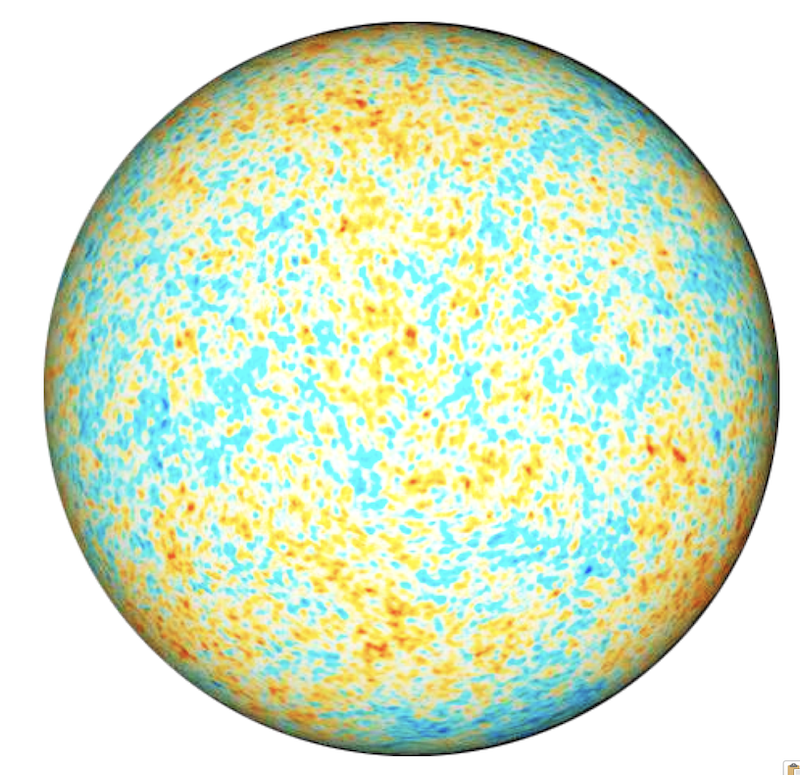
\includegraphics[width=0.9\linewidth]{figures/planck.png}
Cosmic microwave background radiation, captured by the Planck space observatory, is a signal on $\mathbb{S}^2$. 
}
the two-dimensional sphere $\Omega = \mathbb{S}^2$ with the group of rotations, the {\em special orthogonal group} $\fG = \mathrm{SO}(3)$.  
%
While chosen for pedagogical reason, this example is actually very practical and arises in numerous applications. In astrophysics, for example, observational data often naturally has spherical geometry. Furthermore, spherical symmetries are very important in applications in chemistry when modeling molecules and trying to predict their properties, e.g. for the purpose of virtual drug screening.
%\michael{ADD: molecules/astrophysics}


Representing a point on the sphere as a three-dimensional unit vector $\mathbf{u} : \|\mathbf{u}\|=1$, the action of the group can be represented as a $3\times 3$ orthogonal matrix $\mathbf{R}$ with $\mathrm{det}(\mathbf{R}) = 1$. The spherical convolution can thus be written as the inner product between the signal and the rotated filter,
$$
(x\star \theta)(\mathbf{R}) = \int_{\mathbb{S}^2} x(\textbf{u}) \theta(\mathbf{R}^{-1}\mathbf{u}) \mathrm{d}\mathbf{u}.
\marginnote{
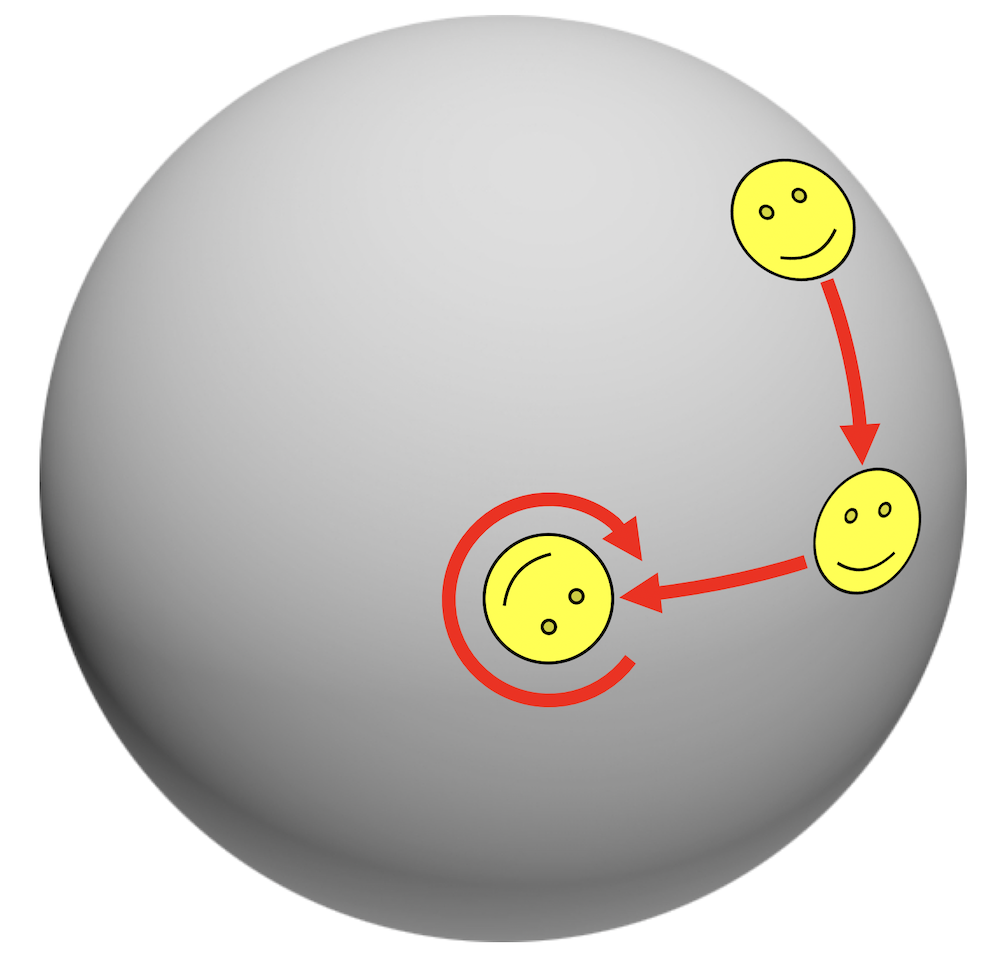
\includegraphics[width=0.9\linewidth]{figures/so3.png}
The action of $\mathrm{SO}(3)$ group on $\mathbb{S}^2$. Note that three types of rotation are possible; the $\mathrm{SO}(3)$ is a three-dimensional manifold.  
}
$$


The first thing to note is than now the group is not identical to the domain: the group $\mathrm{SO}(3)$ is a Lie group that is in fact a three-dimensional manifold, whereas $\mathbb{S}^2$ is a two-dimensional one.  
%
Consequently, in this case, unlike the previous example, the  convolution is a function {\em on} $\SO{3}$ {\em rather than on} $\Omega$. 

%\michael{\bf [ADD: a figure showing the difference between the sphere and SO(3) and why integration on S would give only isotropic filters.]}


This has important practical consequences: in our Geometric Deep Learning blueprint, we concatenate multiple equivariant maps (``layers'' in deep learning jargon) by applying a subsequent operator to the output of the previous one. 
%
In the case of translations, we can apply multiple convolutions in sequence, since their outputs are all defined on the same domain $\Omega$. 
%
In the general setting, since $x \star \theta$ is a function on $\fG$ rather than on $\Omega$, we cannot use exactly the same operation subsequently---it means that the next operation has to deal with {\em signals on $\fG$}, i.e. $x \in \mathcal{X}(\fG)$.  
%
Our definition of group convolution allows this case: 
we take as domain $\Omega = \fG$ acted on by $\fG$ itself via the group action $(\fg, \fh) \mapsto \fg \fh$ defined by the composition operation of $\fG$.
This yields the representation $\rho(\fg)$ acting on $x \in \mathcal{X}(\fG)$  by $(\rho(\fg) x)(\fh) = x(\fg^{-1}\fh)$\marginnote{The representation of $\fG$ acting on functions defined on $\fG$ itself is called the \emph{regular representation} of $\fG$.}.
% where $\fg, \fh$ and their composition $\fg^{-1}\fh$ belong to the group $\fG$.
Just like before, the inner product is defined by integrating the %product of $x$ and $\psi$ 
point-wise product of the signal and the filter 
over the domain, which now equals  $\Omega = \fG$.
%
In our example of spherical convolution, a second layer of convolution would thus have the form
$$
((x\star \theta)\star \phi)(\mathbf{R}) = \int_{\mathrm{SO}(3)} (x\star \theta)(\textbf{Q}) \phi(\mathbf{R}^{-1}\mathbf{Q}) \mathrm{d}\mathbf{Q}.
$$


%Now consider $\Omega = \R^2$ with  the group $\fG = \SE{2}$ of planar rotations and translations.\marginnote{$\SE{2}$ is called the {\em special Euclidean group} and is a subgroup of the Euclidean (isometry) group that additionally includes reflection. } 
%The first thing to note is that now the group elements (roto-translations) are not identical to the points on the domain. Consequently, in this case, unlike the previous example, the group convolution $x\star \psi$ given as the inner product between the signal and the transformed filter is a function {\em on} $\SE{2}$ {\em rather than on} $\Omega$. 

%\taco{TODO: Figure of SE2 group conv. Both planar to group, and group to group.}




%Our construction can be generalized to signals on any (locally compact) group $\fG$ and any $\Omega$ acted on by $\fG$ (in a sufficiently nice way).
%$\Omega$ is said to be a {\em homogeneous space} if for any two points $u, v \in \Omega$ one can be transformed into another, $u = \fg v$, by a symmetry $\fg \in \fG$. 
%that maps one to the other, .
%As noted before, for any such space $\Omega$, we have a regular representation $\rho(\fG)$ of $\fG$ acting on the space of signals $\mathcal{X}(\Omega)$. \michael{Bring the definition of homogeneous space earlier to Sec 1.2.1}
%
%As we will show in Chapter ???, for any two homogeneous spaces $\Omega$ and $\Omega'$ and a group $\fG$, one can define a convolution that maps between $\mathcal{X}(\Omega)$ and $\mathcal{X}(\Omega')$ in an equivariant manner, and indeed the most general linear equivariant map between these spaces is a convolution.

Since convolution involves inner product that in turn requires integrating over the domain $\Omega$, we can only use it on domains $\Omega$ that are small (in the discrete case) or low-dimensional (in the continuous case).  
% 
For instance, we can use convolutions on the plane $\R^2$ (two dimensional) or special orthogonal group $\SE{3}$ (three dimensional), or on the finite set of nodes of a graph ($n$-dimensional), but we cannot in practice perform convolution on the group of permutations $\Sigma_n$, which has $n!$ elements. 
%
Likewise, integrating over higher-dimensional groups like the affine group (containing  translations, rotations, shearing and scaling, for a total of $6$ dimensions) is not feasible in practice. 
%
Nevertheless, as we have seen in Section \ref{sec:gnn-intro}, we can still build equivariant convolutions for large groups $\fG$ by working with signals defined on low-dimensional spaces $\Omega$ on which $\fG$ acts.
Indeed, it is possible to show that any equivariant linear map $f : \mathcal{X}(\Omega) \rightarrow \mathcal{X}(\Omega')$ between two domains $\Omega, \Omega'$ can be written as a generalised convolution similar to the group convolution discussed here. %\michael{Taco: I don't understand what you want to say here.}

Second, we note that the Fourier transform we derived in the previous section from the shift-equivariance property of the convolution can also be extended to a more general case by projecting the signal onto the matrix elements of irreducible representations of the symmetry group. We will discuss this in future work. 
%
In the case of $\SO{3}$ studied here, this gives rise to the {\em spherical harmonics} and {\em Wigner D-functions}, which find wide applications in quantum mechanics and chemistry.


Finally, we point to the assumption that has so far underpinned our discussion in this section: whether $\Omega$ was a grid, plane, or the sphere, we could transform every point into any other point, intuitively meaning that all the points on the domain ``look the same.'' % by means of a rotation  
%
A domain $\Omega$ with such property is called a {\em homogeneous space}, where for any $u, v\in \Omega$ there exists $\mathfrak{g}\in\fG$ such that 
$
\mathfrak{g}.u = v\marginnote{The additional properties, $\mathfrak{e}.u = u$ and $\mathfrak{g} (\mathfrak{h}. u) = (\mathfrak{gh}). u$ are tacitly assumed here. }
$.
%
In the next section we will try to relax this assumption. 

%Consider as given a space $\Omega$, such as $\Omega = \R^2$, $\Omega = \Z^2$, or $\Omega = S^2$ (the sphere).
%Furthermore, let $G$ be a group of symmetries acting on $\Omega$, such as the group of roto-translations acting on $\R^2$, or the group or 3D rotations acting on the sphere.
%The inputs and feature maps of our generalized CNN are modelled as signals on $\Omega$, defined as $\mathcal{X}_\Omega = \{f : \Omega \rightarrow \R\}$\marginnote{In practice one would usually want to use multiple channels $c$, i.e. $f : \Omega \rightarrow \R^c$ but to reduce clutter we consider a single channel / grayscale image for now.}.
%From the action of $G$ on $\Omega$, we can derive an action of $G$ on $\mathcal{X}_\Omega$:
%\begin{equation}
%	\rho(g) f(x) = f(g^{-1} x)
%\end{equation}
%When $G$ is the translation group, this is just the \emph{shift operator} defined in the previous section.
%Similarly, when $G$ is the roto-translation group, this operator tells us how to roto-translate an image of filter $f$.

%In order to match a filter and an image / feature map, we define an inner product:
%\begin{equation}
%    \langle f, \psi \rangle = \int_{\Omega} f(x) \psi(x) d\mu(x),
%\end{equation}
%where $\mu$ is an invariant measure on $\Omega$. % too technical?
%In the case where $\mu$ is discrete, the inner product is a sum over the ``dimensions'' $x$ of the product of the vector components $f(x) \psi(x)$. 

%Having defined how to transform filters and match patterns, we are ready to define the generalized convolution:
%\begin{equation}
%    \label{eq:group-conv}
%    f \star \psi(g) = \langle f, \rho(g) \psi \rangle = \int_\Omega f(x) \psi(g^{-1} x) %d\mu(x).
%\end{equation}

%Let's look at some examples.
%When $\Omega = \Z_n = \{1, \ldots, n\}$ and $G = \Z_n$ (i.e. we consider signals on $\Z_n$ and the group of cyclic shifts) as in the last section, we retrieve the usual discrete convolution.
%To see this, note that $g^{-1} x$ in the equation above means: invert the group element $g \in G$ (in this example, the inverse of $g \in \Z_n$ is $-g$) and then act on $x \in \Omega$ (in this example, we get $x - g$.
%So the equation boils down to $f \star \psi(g) = \sum_i f(i) f(i - g)$.

%Now consider $\Omega = \R^2$ and $G = \SE{2}$, the group of rotations and translations acting on the plane.
%The first thing to note is that $f \star \psi$ is a function on $G = \SE{2}$ rather than a function on $\Omega$.
%In the previous example $\Omega = G$ so the distinction does not matter, but here it does.
%The group convolution computes the similarity between the input and filter for each transformation of the filter.



%Since the feature map $f \star \psi$ is a function on $G$ rather than $\Omega$, we cannot use exactly the same operation for the second and higher layers of the network.
%The solution is easy enough, though: for the second layer we define $\Omega_2 = G$, so that the feature space consists of functions $f : G \rightarrow \R$.
%We again define a shift operator $\rho_2(g)$ acting on such functions by $(\rho(g) f)(h) = f(g^{-1} h)$, where now $g^{-1} h$ refers to composition in the group $G$ (c.f. $g^{-1} x$ for $x \in \Omega$ refering to the group action of $G$ on $\Omega$).
%With these definitions, the exact same Equation \ref{eq:group-conv} defines the group convolution for second and higher layers.

%As a final example, consider spherical CNNs.
%Here we take the domain $\Omega_1 = S^2$ (the sphere) for the input space, and $G = \SO{3}$ the rotation group as symmetries.

%\taco{TODO: all of the above should be more conversational. Maybe focus on one example?}

%\michael{Generalised Fourier transform using representation theory. Bring up again the notion of multidimensional frequencies and show here where it comes from. }


%\michael{{\bf Say something along the lines:} 
%The important difference between the above examples and the case of sets and graphs is that on the grid, plane, or sphere we can represent our group with a small number of parameters: in case case of $\Z_n$, this is just one index, in the case of $\mathbb{R}^2$, this is translation vector and rotation angle, and in the case of the sphere ... 
%
%Conversely, on sets or graphs, the permutation group does not have such a low-dimensional representation and has a combinatorial complexity. 

%Show again why on graphs we don't have multi-dimensional Fourier transform. 
%}

%\michael{Talk about homogeneous vs non-homogenous spaces, using the example of graphs. Make it a segway to the next section}


%[Fourier theory]


\subsection{Geodesics and Manifolds}
\label{sec:geomanifoldsec}
%\michael{\bf [TACO: pls check if you are ok with this narrative. I start with homogeneous spaces, manifolds, then parallel transport. Then we can say that there is a broader view and talk about bundles in general]}

%\joan{
%Some high-level comments on what's written so far. 
%The generalization from groups to gauges is non-trivial, and I think it would be helpful to illustrate this extra level of generality with a running example. 
%In particular, an important innovation is that now we associate input data to certain vector fields on the domain; this is different from before. 
%It seems that this is the setting where the gauge equivariance is best motivated (unless I missed something), and I assume we can still use certain tasks from particle physics to motivate it.
%In other words, so far in our previous applications, the symmetry group acts on signals $\mathcal{X}(\Omega, \gV)$ only through $\Omega$, leaving the channels unchanged (just transporting them along the group action in $\Omega$). Now the situation is different and the gauge transformation is acting on the channels. 
%}

%\joan{I had a quick pass and the section reads very well; the build-up is coherent and objects are introduced keeping the intuition in mind (and adding figures to the margins will be even more helpful. 

%In particular, we can highlight that, contrary to the previous example of a fixed (curved) domain, many applications consider a variable geometric domain, and we wish to obtain signal representations that satisfy certain properties, namely (i) they are intrinsic, ie since the domain is defined only up to isometry, the signal representation should be invariant to isometries, and (ii) stability properties as this geometric domain changes. 
%These two aspects require introducing minimal elements of riemannian geometry 

%I have one comment/question though: currently we introduce the "minimal" elements of riemanian geometry that allow us to define convolutions and to describe the natural symmetries arising in manifold data (in particular isometry). 
%Would it be possible/convenient to highlight the invariance/stability priors early on, to motivate even further the need to introduce the different concepts (connection, parallel transport, isometries, geodesics, etc). In other words, the starting point is that we want to estimate a function $f$ defined over $\gX(\Omega, \R^s)$ that satisfies certain priors. The first and most natural prior is that $f$ is defined up to isometric transformations of $\Omega$. The second (if appropriate) is again the scale separation, ie local statistics in $x \in \gX(\Omega, \R^s)$ dominate. Then we explain how these priors lead again naturally to the GDL template by appropriately extending the notion of convolution. Additionally, it could be pertinent to describe how these priors relate to the stability of $f$ with respect to small changes in the metric structure of $\Omega$. 


%}


In our last example, the %domain $\Omega$ was the 
sphere $\mathbb{S}^2$ \marginnote{As well as the group of rotations $\mathrm{SO}(3)$, by virtue of it being a {\em Lie group}. }
was a {\em manifold}, albeit a special one 
%: every point $u$ on $\mathbb{S}^2$ can be rotated into any other point $v$, intuitively meaning that all the points on the sphere ``look the same.'' % by means of a rotation  
%
%A domain $\Omega$ with such property is called a {\em homogeneous space}, where for any $u, v\in \Omega$ there exists %$\frak{g}\in\fG$ such that 
%$
%\frak{g}.u = v\marginnote{The additional properties, %$\frak{e}.u = u$ and $\frak{g}.(\frak{h}.u) = (\frak{gh}).u$ %are tacitly assumed here. }
%$.
%%
%Homogeneous spaces thus have a 
with a global symmetry group due to its homogeneous structure. 
%
Unfortunately, this is not the case for the majority of manifolds, which typically do not have global symmetries. 
%
In this case, we cannot straightforwardly define an action of $\fG$ on the space of signals on $\Omega$ and use it to `slide' filters around in order to define a convolution as a direct generalisation of the classical construction. 
%. \joan{why would we want to translate signals in the manifold?}
%
Nevertheless, manifolds do have two types of invariance %symmetries
%various kinds of \emph{local} symmetries 
that we will explore in this section: transformations preserving metric structure and local reference frame change.  
%local \emph{gauge symmetries}, which we will now explore. 

While for many machine learning readers manifolds might appear as somewhat exotic objects, they are in fact very common in various scientific domains. In physics, manifolds play a central role as the model of our Universe --- according to Einstein's General Relativity Theory, gravity arises from the curvature of the space-time, modeled as a pseudo-Riemannian manifold.  
%
In more `prosaic' fields such as computer graphics and vision, manifolds are a common mathematical model of 3D shapes.\marginnote{The term `3D' is somewhat misleading and refers to the {\em embedding space}. The shapes themselves are 2D manifolds (surfaces).}  % 
%
The broad spectrum of applications of such models ranges from virtual and augmented reality and 
special effects obtained by means of `motion capture' to structural biology dealing with protein interactions that stick together (`bind' in chemical jargon) like pieces of 3D puzzle. 
%
The common denominator of these applications is the use of a manifold to represent the boundary surface of some 3D object. 


There are several reasons why such models are convenient.\marginnote{
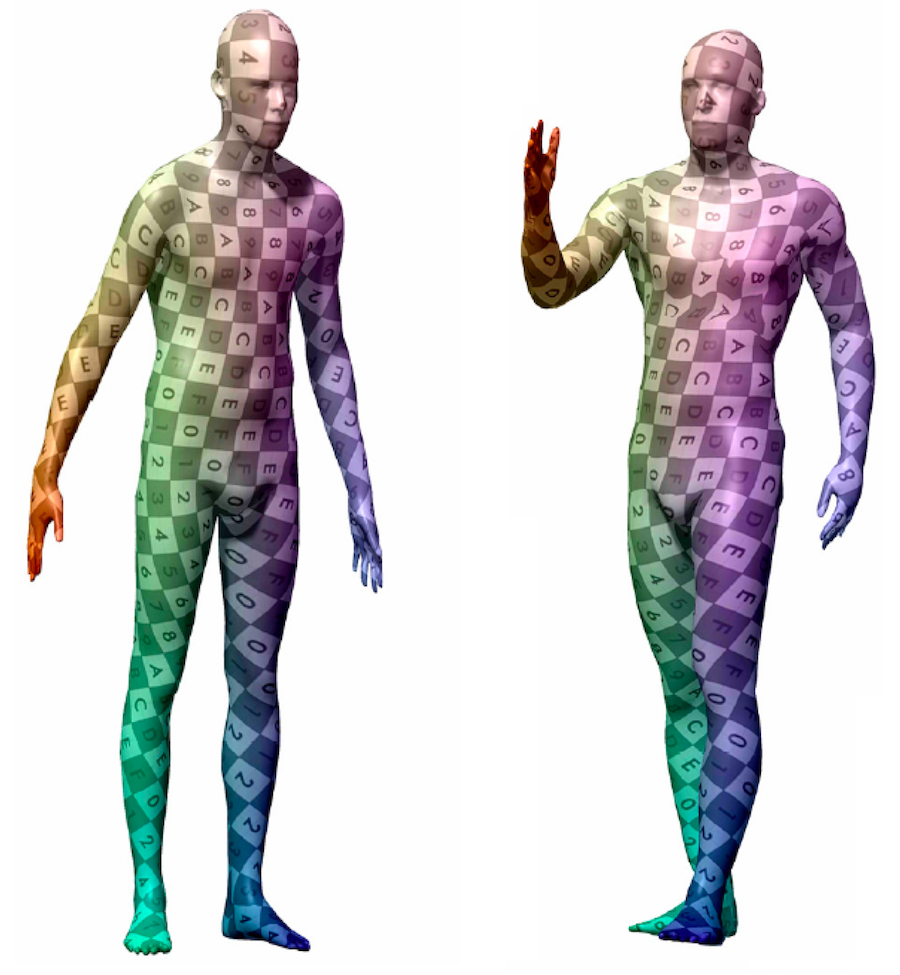
\includegraphics[width=0.9\linewidth]{figures/humans.png}
The human body is an example of a non-rigid object deforming in a  nearly-isometric way. 
} First, they offer a compact description of the 3D object, eliminating the need to allocate memory to `empty space' as is required in grid-based representations. 
%
Second, they allow to ignore the internal structure of the object. This is a handy property for example in structural biology where the internal folding of a protein molecule is often irrelevant for interactions that happen on the molecular surface. 
%
Third and most importantly, one often needs to deal with {\em deformable objects} that undergo non-rigid deformations. Our own body is one such example, and many applications in computer graphics and vision, such as the aforementioned motion capture and virtual avatars, require {\em deformation invariance}.
Such deformations can be modelled very well as transformations that preserve the intrinsic structure of a (Riemannian) manifold, namely the distances between points measured \emph{along} the manifold, without regard to the way the manifold is embedded in the ambient space.

%Here, we should emphasize that 
We should emphasise that %similarly to the case of graphs, 
manifolds fall under the setting of {\em varying domains} in our Geometric Deep Learning blueprint, and in this sense are similar to graphs. We will highlight the importance of the notion of invariance to domain deformations -- what we called `geometric stability' in Section~\ref{sec:geom_stab}. 
%
Since differential geometry is perhaps less familiar to the machine learning audience, we will introduce the basic concepts required for our discussion and refer the reader to \cite{penrose2005road} for their detailed exposition.  

%we have briefly mentioned before. 
%That is, unlike grid of homogeneous spaces we have discussed before where the domain can be assumed fixed and we are concerned with different signals on 

%\taco{Should we clarify why we need manifolds if we want deformation invariance? Also, should we call it deformation insensitivity? Since invariance would imply invariance to arbitrarily large deformations (just compose many small ones, each of which the net is invariant to.)}
%\michael{The proper term is isometry invariance. Isometry is understood in two senses: Riemannian (local metric=quadratic form on tangent space) and metric (geodesic distance). The two are equivalent on geodesically complete spaces due to Hopf-Rinow, which implies we can access the whole manifold through exp map from a single point. }

%\michael{STORY: we want to say that all models we build here are isometry-invariant, by virtue of being intrinsically constructed. This requires the definition of a Riemannian manifold. We can also refer to spectral techniques. 
%
%We then discuss gauges in this perspective, and then say that this is a much broader picture that does not need any metric, nor manifold, and can be defined on a bundle which is a topological construct. 
%}

%\joan{This is a good place to motivate geometric DL models that would fall beyond the homogeneous category: give a representative example that we can use throughout the rest of the section to guide the reader.} \michael{I think we focus this section on the domains, rather than on DL models. We should probably defer it to the discussion of Gauge CNNs.}


%\michael{Taco: why use $s$ and not $d$ for the manifold dimension? Do you want to decouple the feature dimension from the dimension of the manifold? } \joan{I switched from $d$ to $s$ since we used $d$ to refer to the dimensionality of the data and not the intrinsic dimension of the domain}
%
%\paragraph{Riemannian manifolds}
%\label{sec:manifolds}
%
%Since the formal definition of a manifold\marginnote{By `smooth' we mean differentiable suffient number of times, which is tacitly assumed for convenience. `Deformed' here means \emph{diffeomorphic}, i.e., we can map between the two neighbourhoods using a smooth and invertible map with smooth inverse. %, called a diffeomorphism. 
%%In this way, we can choose smooth coordinates for neighbourhoods of the manifold.
%} is somewhat involved, we 
%%defer its detailed discussion to Chapter ??? and 
%prefer to provide an intuitive picture at the expense of some precision. 
%%
%In this context, we can think of a (differentiable or smooth) manifold as a smooth multidimensional curved surface %(or higher dimensional space) 
%that is \emph{locally Euclidean} in the sense that any small neighbourhood around any point it can be deformed
%%\marginnote{`Deformed' here means \emph{homeomorphic to}, i.e. we can map between the neighbourhoods using a continuous and invertible map with continuous inverse. In fact, we will assume the manifold is smooth, in which case the map should be a diffeomorphism -- smooth and invertible with smooth inverse.}
%to a neighbourhood of $\R^s$; 
%%A crucial difference between a manifold\marginnote{We also tacitly assume the manifold to be smooth, i.e. having a $\mathcal{C}^\infty$-differentiable set of transition functions between local spaces.} and a Euclidean space is that a manifold is only {\em locally} Euclidean:  %
%%a small neighbourhood (open set) around each point $u \in \Omega$ is homeomorphic 
%%\marginnote{A {\em homeomorphism} is a continuous map with continuous inverse that preserves topological properties.}  to 
%%(topologically equivalent) to $\mathbb{R}^s$; 
%%
%%by a homeomorphism called a {\em chart}; 
%%the dimension $d$ is that of the manifold, which 
%in this case the manifold is said to be $s$-{\em dimensional}. 
%%
%%The composition of two charts (or more precisely, a chart and an inverse of a chart) allows to transition between the local 
%%
%%
%%Since the manifold is smooth, 
%This allows us to 
%locally approximate the manifold around point $u$ through the \emph{tangent space} $T_u\Omega$.  %and called the {\em tangent space}.
%The latter can be visualized by thinking of a prototypical two-dimensional manifold, the sphere, and attaching a plane to it at a point: with sufficient zoom, the spherical surface will seem planar. 
%% This analogy however should not be taken literally, as manifolds are abstract objects existing on their own without any geometric realization.  % Taco: this may be a bit confusing for newbies
%%
%\marginnote{Formally, the tangent bundle is the {\em disjoint union} $\displaystyle T\Omega = \bigsqcup_{u\in \Omega} T_u\Omega$.} The collection of all tangent spaces is called the {\em tangent bundle}, denoted $T\Omega$; we will dwell on the concept of bundles in more detail in Section~\ref{sec:gauges}. 
%%later and also in Chapter ???.
%
%
%
%A {\em tangent vector}, which we denote by $X\in T_u\Omega$, can be thought of as a local displacement from point $u$. 
%%In order to give it a sense of {\em direction}, 
%In order to measure the \emph{lengths} of tangent vectors and  \emph{angles} between them, %, and {\em volumes}, 
%%
%\marginnote{A bilinear function $g$ is said to be {\em positive-definite} if $g(X,X)>0$ for any non-zero vector $X\neq 0$. If $g$ is expressed as a matrix $\mathbf{G}$, it means $\mathbf{G} \succ 0$. The determinant $|\mathbf{G}|^{1/2}$ provides a local volume element, which does not depend on the choice of the basis. } 
%%
%we need to equip the tangent space with additional structure, expressed as a 
%positive-definite bilinear function
%$g_u: T_u\Omega \times T_u\Omega \rightarrow \mathbb{R}$ depending smoothly on $u$. Such a function is 
%called a {\em Riemannian metric}, in honour of Bernhardt Riemann who introduced the concept in 1856, and can be thought of as an inner product on the tangent space, $\langle X, Y \rangle_u = g_u(X,Y)$, which is an expression of the angle between any two tangent vectors $X, Y \in T_u\Omega$. 
%%
%The metric also induces a norm $\| X \|_u = g_u^{1/2}(X,X)$ allowing to locally measure lengths of vectors. 
%
%
%
%We must stress that tangent vectors 
%\marginnote{Unfortunately, too often vectors are identified with their coordinates. 
%%, which in our view constitutes a crime against humanity. 
%To emphasize this important difference, we use $X$ to denote a tangent vector and $\mathbf{x}$ to denote its coordinates. }
%are abstract geometric entities that exists in its own right and are {\em coordinate-free}. If we are to express a tangent vector $X$ numerically as an array of numbers, we can only represent it as a list of coordinates $\mathbf{x}=(x_1, \hdots, x_s)$ {\em relative to some local basis} $\{ X_1, \hdots X_s \} \subseteq T_u\Omega$.   
%%
%Similarly, the metric can be expressed as an $s\times s$ matrix $\mathbf{G}$ with elements $g_{ij} = g_u(X_i,X_j)$ w.r.t that basis. %; however, we stress that the definition of Riemannian metric does not rely on any particular choice of basis %all our definitions are coordinate-free and exist independently of any basis choice
%%(this will be the centrepiece of the following section). 
%
%%that allows to measure length, angle, and volume in the tangent space. 
%%
%
%
%
%%an {\em inner product}.
%%In differential geometry, an inner product on $T_u\Omega$ depending smoothly on $u$ is called a {\em Riemannian metric}, in honour of Bernhardt Riemann who introduced the concept in 1856. %
%%We will denote a Riemannian metric as a$g_u: T_u\Omega \times T_u\Omega \rightarrow \mathbb{R}$ that allows to measure length, angle, and volume in the tangent space. 
%%
%
%%
%%of a vector $$
%%
%%angle between two tangent vectors $x,y \in T_u\Omega$, (expressed %as $\cos^{-1}\left( \frac{\g_u(x,y)$) and a length of the 
%
%
%A manifold equipped with a metric is called a
%{\em Riemannian manifold} and properties that can be expressed entirely in terms of the metric are said to be {\em intrinsic}. %
%This is a crucial notion for our discussion, as according to our template, we will be seeking to construct functions acting on signals defined on $\Omega$ that are invariant to metric-preserving transformations called {\em isometries} that, roughly speaking, deform the manifold without affecting its local structure. If such functions can be expressed in terms of intrinsic quantities, they are automatically guaranteed to be isometry-invariant and thus unaffected by isometric deformations. 
%%
%These results can be further extended to dealing with approximate isometries; this is thus an instance of the geometric stability (domain deformation) discussed in our blueprint. 
%
%
%%\taco{Taco: here we should probably make clear that we are not talking about symmetries in the sense of automorphisms, i.e. maps $\Omega \rightarrow \Omega$ that preserve the metric, but about isomorphisms, i.e. maps $\Omega \rightarrow \Omega'$ that preserve the metric. Note that we do not yet discuss this in the template, but as discussed we should.} 
%
%%\michael{Approx isometry - geometric stability}
%
%While, as we noted, the definition of a Riemannian manifold does not require a
%geometric realization in any space, it turns out that any smooth Riemannian manifold can be realized as a subset of a Euclidean space of sufficiently high dimension (in which case it is said to be `embedded' in that space) by using the structure of the Euclidean space to induce a Riemannian
%metric.\marginnote{This result is known as the {\em Embedding Theorem}, due to John Forbes Nash, who became a household name after the Hollywood movie The Beautiful Mind. The paper folding art of origami is a manifestation of different isometric embeddings of the planar surface in $\mathbb{R}^3$. \vspace{4mm}
%
\includegraphics[width=1\linewidth]{figures/origami.pdf}
%}  Such an embedding is however not necessarily unique -- as we will see in the following, two different isometric 
%realizations of a Riemannian metric are possible. 
%%called {\em isometries}.
%
%
%
%
%
%\paragraph{Covariant derivative and Parallel transport}
%%
%Since we are interested in signals defined on $\Omega$, we need to provide the proper notion of scalar-
%%\marginnote{We will use the same notation for tangent and vector fields, the distinction between which will be clear from the context.} 
%and vector-valued functions on manifolds. 
%%
%A {\em scalar field} is a function of the form $x: \Omega\rightarrow \mathbb{R}$. 
%%
%%scalar-valued function  (often called a {\em scalar field}) $x: \Omega\rightarrow \mathbb{R}$ on the manifold. The space of 
%Scalar fields form a vector space $\mathcal{X}(\Omega, \mathbb{R})$ that can be equipped with the inner product %of scalar fields
%\begin{equation}
%\langle x, y \rangle = \int_\Omega x(u) y(u) \mathrm{d}u,
%\label{eq:inner_scalar}   
%\end{equation}
%%
%where $\mathrm{d}u$ % = \sqrt{\det g}$
%%\marginnote{More rigorously speaking, the volume form requires an inner product (i.e. Riemannian metric) and {\em orientation} (`handedness'). } 
%is the volume element induced by the Riemannian metric. 
%%
%%
%A (tangent) {\em vector field} is a function of the form $X: \Omega \rightarrow T\Omega$  assigning to each point a tangent vector in the respective tangent space, $u\mapsto X(u)\in T_u\Omega$.  
%%
%Vector fields also form a vector space $\mathcal{X}(\Omega, T\Omega)$ with the inner product defined through the Riemannian metric, 
%%
%\begin{equation}
%\langle X, Y \rangle = \int_\Omega g_u(X(u), Y(u)) \mathrm{d}u. \label{eq:inner_vector}   
%\end{equation}
%
%
%Another way to think of (and actually {\em define}) vector fields is as a generalised notion of derivative. 
%%
%In classical calculus, one can locally linearise a (smooth) function through the {\em differential} $\mathrm{d}x(u) = x(u+\mathrm{d}u) - x(u)$, which provides the change of the value of the function $x$ at point $u$ as a result of an inifinitesimal displacement $\mathrm{d}u$. 
%%
%However, in our case using this  definition na{\"i}vely brings up two problems: First, expressions of the form ``$u+\mathrm{d}u$'' are meaningless on manifolds, since there is no global vector space structure. 
%%, preventing us from adding or subtracting two points on $\Omega$. 
%%
%%
%A second problem arises when trying to take derivatives of vector fields, as one would need to subtract vectors belonging to tangent spaces at {\em different points}, while subtraction is only define \emph{within} a single vector space. 
%
%
%
%
%
%The solution to the first problem is to use tangent vectors as a model of local infinitesimal displacement. 
%%in order to provide a proper generalization of the differential on manifolds. 
%%
%Given a smooth scalar field $x\in \mathcal{X}(\Omega,\mathbb{R})$, we can think of a (smooth) vector field as a linear map $Y:\mathcal{X}(\Omega,\mathbb{R}) \rightarrow \mathcal{X}(\Omega,\mathbb{R})$ satisfying the properties of a {\em derivation}: 
%$Y(c) = 0$ for any constant $c$ (corresponding to the intuition that constant functions have vanishing derivatives), $Y(x+z) = Y(x) + Y(z)$ (linearity), and $Y(xz) = Y(x)z + xY(z)$ ({\em product} or {\em Leibniz rule}), for any smooth scalar fields $x,z \in \mathcal{X}(\Omega,\mathbb{R})$. 
%%
%It can be shown that one can use these properties to define vector fields axiomatically. 
%%
%The differential of $x$ can be defined as an operator $\mathrm{d}x : T\Omega \rightarrow \mathbb{R}$ of the form
%$$
%\mathrm{d}x(Y) = Y(x),
%$$
%which can be interpreted as follows: the change of $x$ as the result of displacement $Y \in T_u\Omega$ at point $u$ is given by $\mathrm{d}x(Y)$. 
%%
%It is thus an extension of the classical notion of {\em directional derivative}. 
%%
%Importantly, this construction {\em does not use the Riemannian metric whatsoever} and can thus be generalised to a broader construction of bundles discussed in the next section. 
%
%
%
%At each point $u$, the differential operator $\mathrm{d}x_u$ can be regarded as a {\em linear functional} acting on tangent vectors $X \in T_u\Omega$. Linear functionals on a vector space are called {\em dual vectors} or {\em covectors}; if in addition we are given an inner product (Riemannian metric), a dual vector can always be represented as 
%\marginnote{This is a consequence of the Riesz-Fr{\'e}chet Representation Theorem, by which every dual vector can be expressed as an inner product with a vector. } 
%$$
%\mathrm{d}x_u (X)  = g_u(\nabla x(u), X).
%$$ 
%The representation of the differential at point $u$ is a tangent vector $\nabla x(u) \in T_u \Omega$ called the (intrinsic) {\em gradient} of $x$; similarly to the gradient in classical calculus, it can be thought of as the direction of the steepest increase of $x$. 
%%
%%More generally, the gradient can be thought of as an operator $\nabla : $
%
%
%
%
%In a similar way, we can axiomatically define the {\em covariant derivative} $\nabla_Y X$ of a smooth vector field $X$ along another smooth vector field $Y$ as an operator  
%$\nabla : T\Omega \times T\Omega \rightarrow T\Omega$ %associating the vector fields $(X,Y) \mapsto \nabla_Y X$ and satisfying the following properties: 
%of the following form:
%
%
%\begin{tcolorbox}[width=\linewidth,
%              boxsep=0pt,
%              left=7.5pt,
%              right=7.5pt,
%              top=7.5pt,
%              bottom=7.5pt,
%              arc=0pt,
%              boxrule=0pt,toprule=0pt,
%              colback=boxgray,
%              ]%%
%A  {\em covariant derivative} (or {\em connection}) is a map $(X,Y) \mapsto \nabla_Y X$
%satisfying, 
%for all smooth scalar fields $x, y \in \mathcal{X}(\Omega, \mathbb{R})$ and smooth vector fields $X, Y, Z \in \mathcal{X}(\Omega, T\Omega)$, 
%the following axioms: \vspace{3mm}\\
%%\begin{enumerate}
%%\item 
%\noindent {\em Linearity (w.r.t. first argument):} 
%$\nabla_{xY + yZ}(X) = \nabla_Y(X)x + \nabla_Z(X)y$.\vspace{2mm}\\
%\noindent  {\em Additivity (w.r.t. second argument):}
%%\marginnote{For an {\em affine connection}, the additivity requirement is dropped. } 
%$\nabla_Y(X+Z) = \nabla_Y X + \nabla_Y Z$.\vspace{2mm}\\
%\noindent  {\em Product rule:} $\nabla_Y(zX) = z \nabla_Y(X) + \mathrm{d}z(Y) X$, where for scalar fields the covariant derivative coincides with the differential,  
%%, where in the second term  
%$\nabla_Y(z) = \mathrm{d}z(Y)$.%\vspace{2mm}
%%
%%    \noindent  
%%\end{enumerate}
%
%\end{tcolorbox}
%
%Covariant derivative allows {\em parallel transport}, or a way of moving tangent vectors along a curve so they are ``pointing in the same direction''.  
%%
%Given a smooth curve $\gamma : [0,T] \rightarrow \Omega$, a vector $X$ is said to be parallel transported along $\gamma$ if $\nabla_{\gamma'(t)} X(\gamma(t)) = 0$ for $t \in [0,T]$, where $\gamma'(t) \in T_{\gamma(t)} \Omega$ is the tangent to the curve. 
%%
%Intuitively, this implies that the vector remains `constant'\marginnote{
%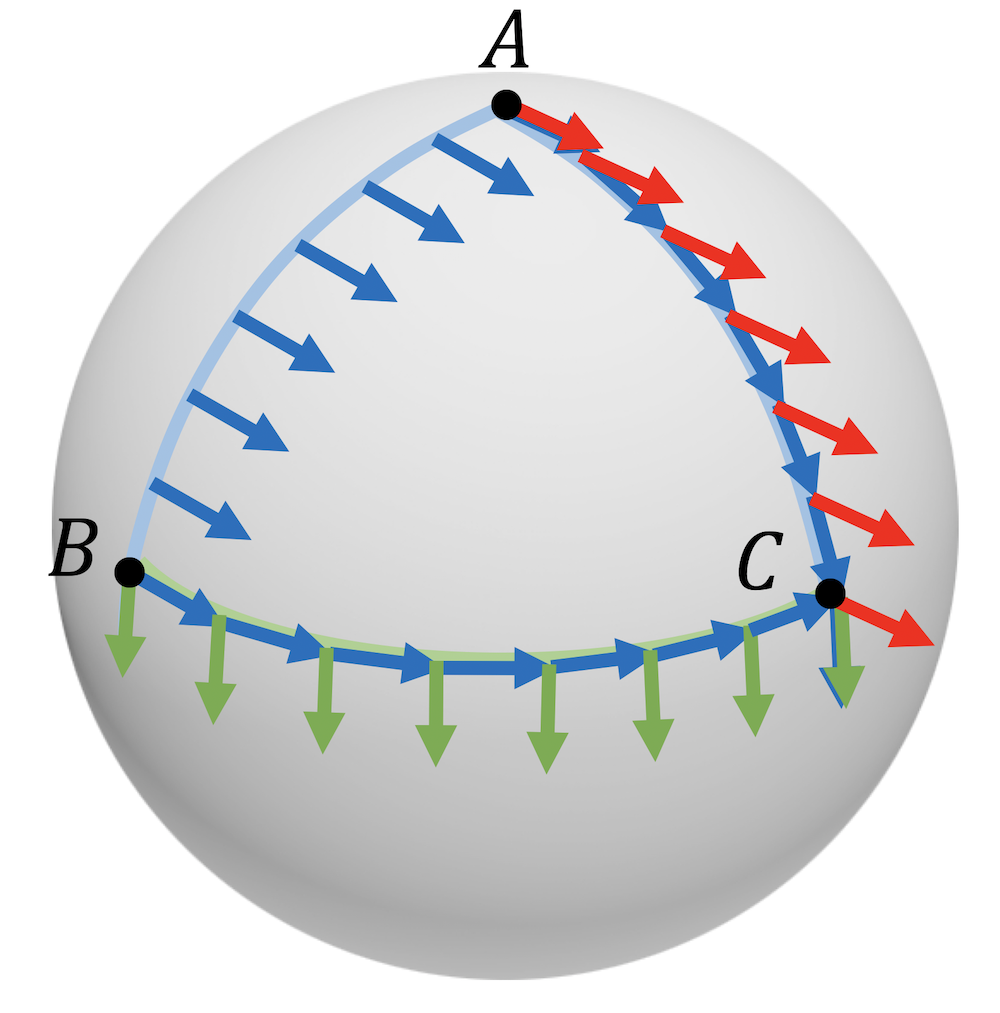
\includegraphics[width=0.9\linewidth]{figures/parallel.png}
%Euclidean transport of a vector from A to C makes no sense on the sphere, as the resulting vectors (red) are not in the tangent plane. Parallel transport from A to C (blue) rotates the vector along the path. It is path dependent: going along the path BC and ABC produces different results.  
%} (the derivative vanishes) for a small displacement along the curve. 
%%
%The result of the transport is path-dependent, which is best visualised on the sphere (see insert): moving a vector from the north pole to the equator along two different curves produces different results.
%%
%The name `connection' stems from the fact that parallel transport defines a linear isomorphism between tangent spaces along the curve $\gamma$, that is, a way to transport vectors from $T_{\gamma(0)}\Omega$ to $T_{\gamma(T)}\Omega$, thereby `connecting' these spaces.
%
%
%%which transports its tangent along itself 
%
%
%%perform  
%%of tangent vectors by (in this way, it ``connects'' two tangent spaces at different points, hence the alternative name `connection').  
%
%It is important to note that the definition of the covariant derivative  %and geodesic 
%does not rely on the metric, and  
%in fact, is an abstract construction that extends beyond Riemannian manifolds. %there are multiple ways to define one.  
%%
%When one is given a Riemannian metric, of particular interest is a special kind of covariant derivative called the {\em Levi-Civita connection}, after the Italian mathematician Tullio Levi-Civita who introduced the notion in 1917. %\marginnote{}
%%
%
%
%\begin{tcolorbox}[width=\linewidth,
%              boxsep=0pt,
%              left=7.5pt,
%              right=7.5pt,
%              top=7.5pt,
%              bottom=7.5pt,
%              arc=0pt,
%              boxrule=0pt,toprule=0pt,
%              colback=boxgray,
%              ]%%
%The {\em Levi-Civita connection} on a Riemannian manifold with metric $g$ is a connection $\nabla$ that additionally satisfies the following properties:
%\vspace{3mm}\\
%%\begin{enumerate}
%%\item 
%    \noindent  {\em Torsion free:} \marginnote{Roughly, {\em torsion} describes how tangent vectors twist about the curve when parallel transported, and {\em curvature} how they roll along it. }
%$\nabla_X Y - \nabla_Y X = [X,Y]$, where the tangent vector field $[X,Y] \in \mathcal{X}(\Omega, T\Omega)$ is the 
%{\em commutator} (also known as the {\em Lie bracket} or {\em Lie derivative}), defined by its action on scalar fields 
%$$[X,Y](z) = X(Y(z)) - Y(X(z)).$$
%%\vspace{2mm}\\
%%    
%\noindent {\em Preserves the metric:}\marginnote{Connection with this property is also known as {\em metric} or {\em metric-compatible}.} 
%$\nabla g = 0$, which is understood as 
%$$
%(\nabla_X g)(Y,Z) = X(g(Y,Z)) - g(\nabla_X Y, Z) - g(Y, \nabla_X Z) = 0.
%$$
%for any smooth $X, Y$, and $Z$. 
%
%\end{tcolorbox}
%
%
%%
%%
%The condition $\nabla g = 0$ (metric compability) implies that the metric remains invariant under parallel transport, i.e., parallel transport preserves the length of the tangent vectors (and is thus an isometry). 
%%
%The torsion-free properties make the Levi-Civita connection {\em unique}, a result known as the Fundamental Theorem of Riemannian Geometry. 
%%
%%\marginnote{
%For this reason, in Riemannian geometry the term `connection' is usually synonymous with the Levi-Civita connection, which can be considered a `canonical' connection.
%
%%guaranteeing that every Riemannian manifold admits a unique Levi-Civita connection, making it thus the `canonical' one. 
%
%
%
%
%%\taco{I think the notion of Torsion will be difficult to understand for newbies. Also, we are differentiating a tensor field g which I think we have not explained yet.
%
%%We could consider just mentioning the LC connection and explaining that parallel transport defined wrt it will not change the length of tangent vectors. We can also say that if another condition (Torsion free) is satisfied, there is a unique LC connection, without formalizing it.}
%
%
%
%\paragraph{Geodesics and Exponential map}
%
%A curve $\gamma$ along which parallel transport preserves the tangent vector to the curve,\marginnote{From the Greek \textgreek{geodai\textsigma{}{\'i}a}, literally `division of Earth'.}  i.e., $\nabla_{\gamma'} \gamma' = 0$ is called {\em geodesic}.
%%
%Locally at a point $u$, it is always possible to define a unique geodesic in a given direction $X$, i.e. a smooth curve $\gamma_X : [0,T] \rightarrow \Omega$ satisfying $\gamma(0) = u$ and $\gamma'(0) = X$, for some small $T>0$. 
%%
%%
%This\marginnote{Here, $B_r(0)$ is a ball of radius $r$ around the origin. Note that geodesic completeness does not necessarily guarantee that $\exp$ is a diffeomorphism -- the largest radius $r$ about $u$ for which $\exp_u(B_r(0) \subseteq T_u\Omega)$ is mapped diffeomorphically is called the {\em injectivity radius}. } gives a natural mapping from (a subset of) the tangent space $T_u \Omega$ to $\Omega$ called the {\em exponential map} $\exp : B_r(0) \subset T_u\Omega \rightarrow \Omega$, which is defined by taking a unit step along the geodesic in the direction $X$, i.e., $\exp_u(X) = \gamma_X(1)$. %
%%
%%
%When $\gamma_X(t)$ is defined for all $t\geq 0$ (that is, we can shoot the geodesic from a point $u$ for as long as we like), the manifold is said to be {\em geodesically complete} and the exponential map is defined on the whole tangent space.
%%
%Since compact manifolds are geodesically complete, we can tacitly assume this convenient property. 
%
%
%
%%
%On Riemannian\marginnote{It is tacitly assumed that curves are given in {\em arclength parametrisation}, such that $\| \gamma' \| = 1$ (constant velocity).} manifolds with the Levi-Civita connection, one can show geodesics to be {\em length-minimising curve}, 
%%
%i.e., a geodesic $\gamma$ minimises the length functional 
%%
%$$
%L(\gamma) = \int_{0}^T \| \gamma'(t) \| \mathrm{d}t =  \int_{0}^T g_u^{1/2} (\gamma'(t), \gamma'(t)) \mathrm{d}t 
%$$
%%
%among all curves with endpoints $u = \gamma(0)$ and $v=\gamma(T)$. 
%%
%%
%Readers familiar with metric geometry are probably more used to this definition of geodesics as shortests paths. 
%%
%In fact, \marginnote{Hopf-Rinow Theorem thus estabilishes the equivalence between geodesic and metric completeness, the latter meaning every Cauchy sequence converges.} a result known as the Hopf-Rinow Theorem guarantees that geodesically complete manifolds are also {\em complete metric spaces}, in which one can realise a metric (called the {\em geodesic distance})  between any pair of points $u,v$ as the length of the shortest path between them
%$$
%d_g(u,v) = \min_{\gamma} L(\gamma) \quad\quad \text{s.t.} \quad\quad \gamma(0) = u, \,\, \gamma(T) = v,
%$$
%which exists (i.e., the minimum is attained).\marginnote{To avoid confusion with the Riemannian metric, we will use the term `distance'. Our notation $d_g$ makes the distance depend on the Riemannian metric, though the definition of $L$. }
%%
%Importantly, geodesic distances are intrinsic, being dependent solely on the Riemannian metric. 
%
%
%%The term `geodesic' is also used in metric geometry, where it is defined as the shortest path. In the setting described here the two meanings coincide. }
%
%
%%i.e., the two notions of `geodesic' used somewhat differently in differential and metric geometry
%
%
%
%
%
%%===
%%
%%
%%For a smooth scalar field\marginnote{Linear functionals acting on vectors are called {\em dual vectors} or {\em covectors}. By the Riesz-Fr{\'e}chet Representation Theorem, every covector can be expressed as an inner product with a vector. } $x: \Omega \rightarrow \mathbb{R}$, the differential can be thought of as an operator $dx : T\Omega \rightarrow \mathbb{R}$ acting on tangent fields. At each point, the differential can be expressed as a linear functional acting on tangent vectors
%%$dx(u)  = g_u(\nabla x(u), \cdot)$. 
%%%
%%%
%%Given a smooth vector field $Y$, 
%%the {\em covariant derivative} $\nabla_Y x$ of $x$ {\em along} $Y$ is defined as 
%%$(\nabla_Y x)(u) = g_u(\nabla x(u), Y(u))$
%%and is a generalisation of the corresponding notion in classical calculus. 
%%%
%%%The change of the value of $x$ as the result of 
%%%displacement $y \in T_u\Omega$ at point $u$ is thus given by applying the form to the tangent
%%%vector, $dx(u) y = g_u(\nabla x(u), y)$, and can be thought
%%%of as an extension of the notion of the classical directional
%%%derivative.
%%%
%%The vector field $\nabla x$ is called the (intrinsic) {\em gradient} of $x$; at each point, it indicates the direction of the steepest increase of $x$. 
%%%
%%%The symbol $\nabla$ can be though of as an operator acting on scalar fields and producing vector fields defined above.  
%%
%%
%%Given two smooth vector fields $x$ and $y$, the covariant derivative $\nabla_y x$ of $x$ along $y$
%%
%%
%%
%%
%%Connection is defined as an abstract map $\nabla : T\Omega \times T\Omega \rightarrow T\Omega$ associating $(x,y) \mapsto \nabla_y x$ in a way that is linear w.r.t. both $x$ and $y$ and also satisfies the {\em product rule} $\nabla_y(xz) = x\nabla_y z + z \nabla_y x$ for any vector fields $x,y$ and scalar field $z$. 
%%
%%
%%
%%When the manifold is embedded in a Euclidean space, the covariant derivative coincides with the standard Euclidean directional derivarive projected onto the tangent space. 
%%
%%
%%
%%
%%
%%
%%%known as the {\em pushforward} $d\eta : T\Omega \rightarrow T\Omega'$.  
%%
%%
%%
%%the notion of derivative describes how the value of a function changes with an infinitesimal change of its
%%argument. 
%%
%%
%%One of the big differences distinguishing classical
%%calculus from differential geometry is a lack of vector space
%%
%%
%%structure on the manifold, prohibiting us from na\"{i}vely using
%%expressions like $f(x+dx)$. The conceptual leap that is required
%%to generalize such notions to manifolds is the need to work
%%locally in the tangent space
%%
%%
%%
%%
%%
%%
%%
%%
%%
%%
%
%
%
%
%
%\paragraph{Isometries}
%Consider now a deformation of our manifold $\Omega$ into another manifold $\Omega'$ with a Riemannian metric $h$.
%%
%We will assume this map to be a diffeomorphism $\eta: (\Omega, g) \rightarrow (\Omega', h)$ between manifolds.   
%%
%Its differential $\mathrm{d}\eta : T\Omega \rightarrow T\Omega'$ defines a map between the respective tangent bundles (referred to as {\em pushforward}), such that   
%%\marginnote{The pushforward is what is called a {\em bundle map}.}
%at a point $u$, we have $\mathrm{d}\eta_u : T_u \Omega \rightarrow T_{\eta(u)}\Omega'$, %which allows to interpret it as follows: 
%%
%interpreted as before: 
%if we make a small displacement from point $u$ by tangent vector $X \in T_u \Omega$, the map $\eta$ will be displaced from point $\eta(u)$ by tangent vector $\mathrm{d}\eta_u(X) \in T_{\eta(u)}\Omega'$. 
%
%
%Since the pushforward provides a mechanism to associate tangent vectors on the two manifolds, it allows to {\em pullback }\marginnote{Pushforward and pullback are adjoint operators $\langle \eta^* \alpha, X \rangle = \langle \alpha, \eta_*X \rangle$ where $\alpha \in T^*\Omega$ is a {\em dual vector field}, defined at each point as a linear functional acting on $T_u\Omega$ and the inner products are defined respectively on vector and dual vector fields. } the metric $h$ from $\Omega'$ to $\Omega$, 
%$$
%(\eta^*h)_u(X,Y) = h_{\eta(u)}(\mathrm{d}\eta_u(X), \mathrm{d}\eta_u(Y))
%$$ 
%%
%If the pullback metric coincides at every point with that of $\Omega$, i.e., $g = \eta^*h$, the map $\eta$ is called  (a Riemannian) {\em isometry}. % (metric-preserving). 
%%
%For two-dimensional manifolds (surfaces), isometries can be intuitively understood as inelastic deformations that deform the manifold without `stretching' or `tearing' it. 
%
%
%
%By virtue of their definition, isometries preserve intrinsic structures such as geodesic distances, which are expressed entirely in terms of the Riemannian metric. % and Gaussian curvature.
%%
%Therefore, we can also understand isometries from the position of metric geometry,\marginnote{The Myers–Steenrod Theorem establishes that the converse is also true on connected manifolds: every metric isometry is also a Riemannian isometry. } 
%as distance-preserving maps {\em between metric spaces} $\eta : (\Omega, d_g) \rightarrow (\Omega', d_h)$, in the sense that 
%$$
%d_g (u,v) = d_h(\eta(u),\eta(v)) 
%$$
%for all $u,v \in \Omega$, 
%or more compactly, $d_g = d_h \circ (\eta \times \eta)$. 
%%where $d_g, d_g$ are the geodesic distances induced by the respective Riemannian metrics $g, h$. 
%%
%
%%[Gauss Theorema Egregium, definition of curvature through perimeter defect, pizza example]
%
%
%A particular case of the above is a diffeomorphism  of the domain itself, which we will denote by $\tau \in \mathrm{Diff}(\Omega)$. We will call it a Riemannian  \mbox{(self-)isometry} if the pullback metric satisfies $\tau^* g = g$, or a metric (self-)isometry if $d_g = d_g\circ (\tau \times \tau)$.
%%
%Not surprisingly, isometries form a group with the composition operator denoted by $\mathrm{Iso}(\Omega)$ and called the {\em isometry group}; the identity element is the map $\tau(u) = u$ and the inverse always exists (by definition of $\tau$ as a diffeomorphism). 
%%
%Self-isometries are thus {\em intrinsic symmetries} of manifolds.
%
%
%%Continuous symmetries on manifolds are infinitesimally generated
%%%\marginnote{More correctly, Killing fields are the infinitesimal generators of continuous symmetries. } 
%%by special tangent vector fields called {\em Killing fields}, named after Wilhelm Killing. A field $X$ is Killing if the  Lie derivative\marginnote{The Lie derivative in this case is a derivative of forms. For scalar and vector fields, it coincides with the covariant derivative $\mathcal{L}_X y = \nabla_X y$ and the commutator $\mathcal{L}_X Y = [X,Y]$, respectively. } of the Riemannian metric along it vanishes, $\mathcal{L}_X g = 0$, which is interpreted as 
%%%
%%$$
%%\mathcal{L}_X g(Y,Z) = g(\nabla_Y X, Z) + g(Y,\nabla_Z X) = 0
%%$$
%%for any smooth tangent fields $Y, Z$. 
%%%
%%We can recap that like we mentioned in Section~\ref{sec:symmetries}, we can regard symmetries as automorphisms (self-maps) preserving additional structure: either the local Riemannian metric, or global geodesic distances between pairs of points. 
%%%\taco{Do we need Killing fields? It's interesting but I worry that we'd need to properly introduce Lie derivatives to make it understandable.} \michael{Lets keep them for now}
%%%OK :)
%



\paragraph{Riemannian manifolds}
\label{sec:manifolds}

Since the formal definition of a manifold\marginnote{By `smooth' we mean differentiable suffient number of times, which is tacitly assumed for convenience. `Deformed' here means \emph{diffeomorphic}, i.e., we can map between the two neighbourhoods using a smooth and invertible map with smooth inverse. %, called a diffeomorphism. 
%In this way, we can choose smooth coordinates for neighbourhoods of the manifold.
} is somewhat involved, we 
%defer its detailed discussion to Chapter ??? and 
prefer to provide an intuitive picture at the expense of some precision. 
%
In this context, we can think of a (differentiable or smooth) manifold as a smooth multidimensional curved surface %(or higher dimensional space) 
that is \emph{locally Euclidean}, in the sense that any small neighbourhood around any point it can be deformed
%\marginnote{`Deformed' here means \emph{homeomorphic to}, i.e. we can map between the neighbourhoods using a continuous and invertible map with continuous inverse. In fact, we will assume the manifold is smooth, in which case the map should be a diffeomorphism -- smooth and invertible with smooth inverse.}
to a neighbourhood of $\R^s$; 
%A crucial difference between a manifold\marginnote{We also tacitly assume the manifold to be smooth, i.e. having a $\mathcal{C}^\infty$-differentiable set of transition functions between local spaces.} and a Euclidean space is that a manifold is only {\em locally} Euclidean:  %
%a small neighbourhood (open set) around each point $u \in \Omega$ is homeomorphic 
%\marginnote{A {\em homeomorphism} is a continuous map with continuous inverse that preserves topological properties.}  to 
%(topologically equivalent) to $\mathbb{R}^s$; 
%
%by a homeomorphism called a {\em chart}; 
%the dimension $d$ is that of the manifold, which 
in this case the manifold is said to be $s$-{\em dimensional}. 
%
%The composition of two charts (or more precisely, a chart and an inverse of a chart) allows to transition between the local 
%
%
%Since the manifold is smooth, 
This allows us to 
locally approximate the manifold around point $u$ through the \emph{tangent space} $T_u\Omega$.  %and called the {\em tangent space}.
The latter can be visualised by thinking of a prototypical two-dimensional manifold, the sphere, and attaching a plane to it at a point: with sufficient zoom, the spherical surface will seem planar (Figure~\ref{fig:sphere_metric}). 
% This analogy however should not be taken literally, as manifolds are abstract objects existing on their own without any geometric realization.  % Taco: this may be a bit confusing for newbies
%
\marginnote{Formally, the tangent bundle is the {\em disjoint union} $\displaystyle T\Omega = \bigsqcup_{u\in \Omega} T_u\Omega$.} The collection of all tangent spaces is called the {\em tangent bundle}, denoted $T\Omega$; we will dwell on the concept of bundles in more detail in Section~\ref{sec:gauges}. 
%later and also in Chapter ???.



A {\em tangent vector}, which we denote by $X\in T_u\Omega$, can be thought of as a local displacement from point $u$. 
%In order to give it a sense of {\em direction}, 
In order to measure the \emph{lengths} of tangent vectors and  \emph{angles} between them, %, and {\em volumes}, 
%
\marginnote{A bilinear function $g$ is said to be {\em positive-definite} if $g(X,X)>0$ for any non-zero vector $X\neq 0$. If $g$ is expressed as a matrix $\mathbf{G}$, it means $\mathbf{G} \succ 0$. The determinant $|\mathbf{G}|^{1/2}$ provides a local volume element, which does not depend on the choice of the basis. } 
%
we need to equip the tangent space with additional structure, expressed as a 
positive-definite bilinear function
$g_u: T_u\Omega \times T_u\Omega \rightarrow \mathbb{R}$ depending smoothly on $u$. Such a function is 
called a {\em Riemannian metric}, in honour of Bernhardt Riemann who introduced the concept in 1856, and can be thought of as an inner product on the tangent space, $\langle X, Y \rangle_u = g_u(X,Y)$, which is an expression of the angle between any two tangent vectors $X, Y \in T_u\Omega$. 
%
The metric also induces a norm $\| X \|_u = g_u^{1/2}(X,X)$ allowing to locally measure lengths of vectors. 



We must stress that tangent vectors 
are abstract geometric entities that exists in their own right and are {\em coordinate-free}. If we are to express a tangent vector $X$ numerically as an array of numbers, we can only represent it as a list of coordinates $\mathbf{x}=(x_1, \hdots, x_s)$ {\em relative to some local basis}\marginnote{Unfortunately, too often vectors are identified with their coordinates. 
%, which in our view constitutes a crime against humanity. 
To emphasise this important difference, we use $X$ to denote a tangent vector and $\mathbf{x}$ to denote its coordinates. } $\{ X_1, \hdots X_s \} \subseteq T_u\Omega$.   
%
Similarly, the metric can be expressed as an $s\times s$ matrix $\mathbf{G}$ with elements $g_{ij} = g_u(X_i,X_j)$ in that basis. 
%
We will return to this point in Section~\ref{sec:gauges}. 
%; however, we stress that the definition of Riemannian metric does not rely on any particular choice of basis %all our definitions are coordinate-free and exist independently of any basis choice
%(this will be the centrepiece of the following section). 

%that allows to measure length, angle, and volume in the tangent space. 
%

%\michael{Add a simple example here}


\begin{figure}[h!]
    \centering
    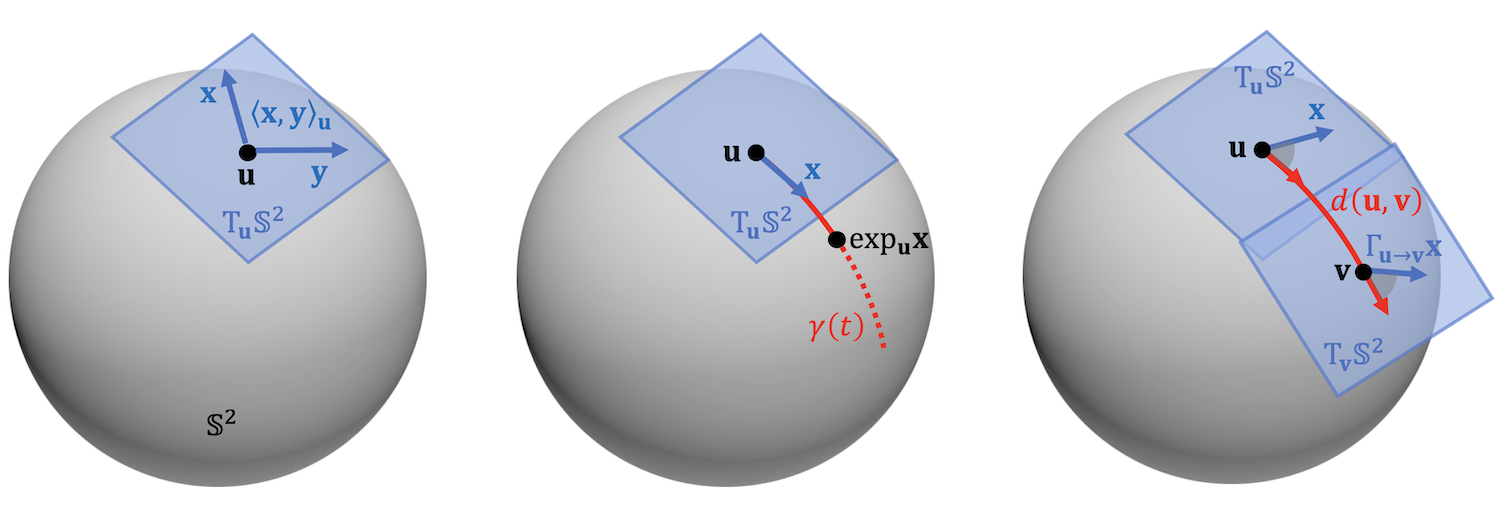
\includegraphics[width=\linewidth]{figures/manifold.png}
    \caption{
    Basic notions of Riemannian geometry illustrated on the example of the two-dimensional sphere $\mathbb{S}^2 = \{\mathbf{u}\in \mathbb{R}^3 : \|\mathbf{u}\|=1 \}$, realised a subset (sub-manifold) of $\mathbb{R}^3$. 
%
The tangent space to the sphere is given as $T_\mathbf{u}\mathbb{S}^2 = \{ \mathbf{x}\in \mathbb{R}^3 : \mathbf{x}^\top \mathbf{u} = 0\}$ and is a 2D plane -- hence this is a 2-dimensional manifold. The Riemannian metric is simply the Euclidean inner product restricted to the tangent plane, $\langle \mathbf{x}, \mathbf{y}\rangle_\mathbf{u} = \mathbf{x}^\top \mathbf{y}$ for any $\mathbf{x},\mathbf{x}\in T_\mathbf{u}\mathbb{S}^2$. 
The exponential map is given by 
$\exp_\mathbf{u}(\mathbf{x}) = \cos(\| \mathbf{x}\|)\mathbf{u} + \frac{\sin(\| \mathbf{x}\|)}{\|\mathbf{x}\|} \mathbf{x}$, for $\mathbf{x} \in T_\mathbf{u}\mathbb{S}^2$. 
%
Geodesics are great arcs of length $d(\mathbf{u},\mathbf{v}) = \cos^{-1}(\mathbf{u}^\top \mathbf{v})$.
    }
    \label{fig:sphere_metric}
\end{figure}%


%an {\em inner product}.
%In differential geometry, an inner product on $T_u\Omega$ depending smoothly on $u$ is called a {\em Riemannian metric}, in honour of Bernhardt Riemann who introduced the concept in 1856. %
%We will denote a Riemannian metric as a$g_u: T_u\Omega \times T_u\Omega \rightarrow \mathbb{R}$ that allows to measure length, angle, and volume in the tangent space. 
%

%
%of a vector $$
%
%angle between two tangent vectors $x,y \in T_u\Omega$, (expressed %as $\cos^{-1}\left( \frac{\g_u(x,y)$) and a length of the 


A manifold equipped with a metric is called a
{\em Riemannian manifold} and properties that can be expressed entirely in terms of the metric are said to be {\em intrinsic}. %
This is a crucial notion for our discussion, as according to our template, we will be seeking to construct functions acting on signals defined on $\Omega$ that are invariant to metric-preserving transformations called {\em isometries} that deform the manifold without affecting its local structure.\marginnote{

\includegraphics[width=1\linewidth]{figures/origami.pdf}
This result is known as the {\em Embedding Theorem}, due to 
\cite{nash1971imbedding}.
%John Forbes Nash, who became a household name after the Hollywood movie The Beautiful Mind. 
The %paper folding 
art of origami is a manifestation of different isometric embeddings of the planar surface in $\mathbb{R}^3$ (Figure: Shutterstock/300 librarians). 
}  If such functions can be expressed in terms of intrinsic quantities, they are automatically guaranteed to be isometry-invariant and thus unaffected by isometric deformations. 
%
These results can be further extended to dealing with approximate isometries; this is thus an instance of the geometric stability (domain deformation) discussed in our blueprint. 


%\taco{Taco: here we should probably make clear that we are not talking about symmetries in the sense of automorphisms, i.e. maps $\Omega \rightarrow \Omega$ that preserve the metric, but about isomorphisms, i.e. maps $\Omega \rightarrow \Omega'$ that preserve the metric. Note that we do not yet discuss this in the template, but as discussed we should.} 

%\michael{Approx isometry - geometric stability}

While, as we noted, the definition of a Riemannian manifold does not require a
geometric realisation in any space, it turns out that any smooth Riemannian manifold can be realised as a subset of a Euclidean space of sufficiently high dimension (in which case it is said to be `embedded' in that space) by using the structure of the Euclidean space to induce a Riemannian
metric. Such an embedding is however not necessarily unique -- as we will see, two different isometric 
realisations of a Riemannian metric are possible. 
%called {\em isometries}.



%\joan{Consider a transition paragraph here, where we explain that we introduce the minimal elements of differential geometry that lead to the key notion of isometry and geodesics}



\paragraph{Scalar and Vector fields}
%
Since we are interested in signals defined on $\Omega$, we need to provide the proper notion of scalar-
%\marginnote{We will use the same notation for tangent and vector fields, the distinction between which will be clear from the context.} 
and vector-valued functions on manifolds. 
%
A (smooth) {\em scalar field} is a function of the form $x: \Omega\rightarrow \mathbb{R}$. \marginnote{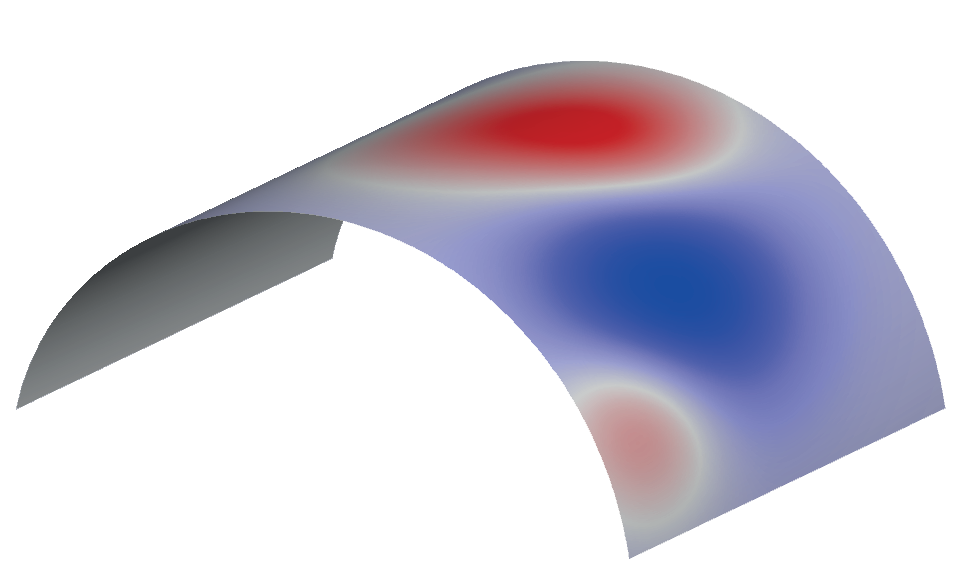
\includegraphics[width=0.9\linewidth]{figures/field_scalar.pdf}\\
Example of a scalar field. 
}
%\marginnote{The fields are typically assumed to be of the same regularity class (smoothness) as the manifold itself. }
%
%scalar-valued function  (often called a {\em scalar field}) $x: \Omega\rightarrow \mathbb{R}$ on the manifold. The space of 
Scalar fields form a vector space $\mathcal{X}(\Omega, \mathbb{R})$ that can be equipped with the inner product %of scalar fields
\begin{equation}
\langle x, y \rangle = \int_\Omega x(u) y(u) \mathrm{d}u,
\label{eq:inner_scalar}   
\end{equation}
%
where $\mathrm{d}u$ % = \sqrt{\det g}$
%\marginnote{More rigorously speaking, the volume form requires an inner product (i.e. Riemannian metric) and {\em orientation} (`handedness'). } 
is the volume element induced by the Riemannian metric. 
%
%
A (smooth) {\em tangent vector field} is a function of the form $X: \Omega \rightarrow T\Omega$  assigning to each point a tangent vector in the respective tangent space, $u\mapsto X(u)\in T_u\Omega$.  
%
Vector fields\marginnote{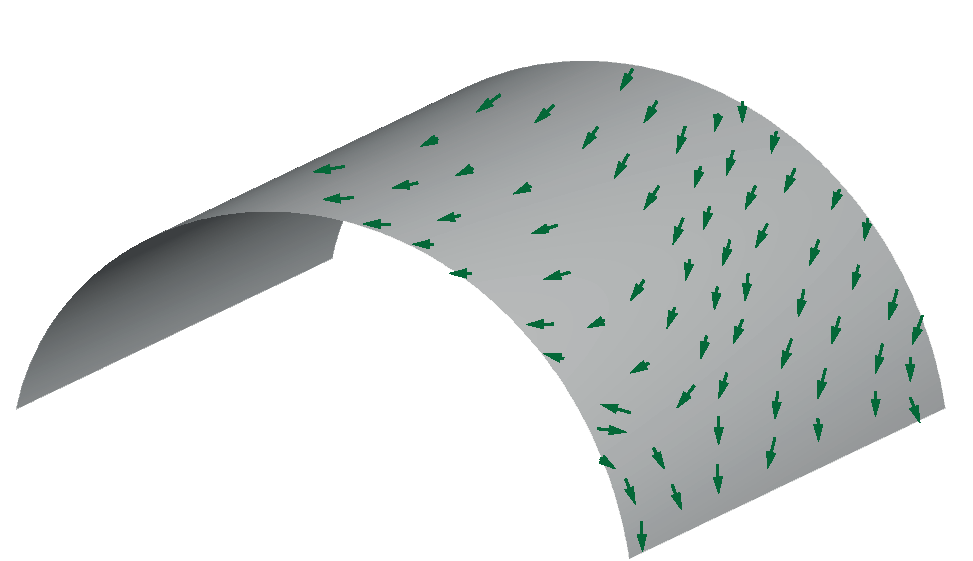
\includegraphics[width=0.9\linewidth]{figures/field_vector.pdf}\\
Example of a vector field. The fields are typically assumed to be of the same regularity class (smoothness) as the manifold itself.
} also form a vector space $\mathcal{X}(\Omega, T\Omega)$ with the inner product defined through the Riemannian metric, 
%
\begin{equation}
\langle X, Y \rangle = \int_\Omega g_u(X(u), Y(u)) \mathrm{d}u. \label{eq:inner_vector}   
\end{equation}


\paragraph{Intrinsic gradient}
Another way to think of (and actually {\em define}) vector fields is as a generalised notion of derivative. 
%
In classical calculus, one can locally linearise a (smooth) function through the {\em differential} $\mathrm{d}x(u) = x(u+\mathrm{d}u) - x(u)$, which provides the change of the value of the function $x$ at point $u$ as a result of an inifinitesimal displacement $\mathrm{d}u$. 
%
However, in our case the na{\"i}ve use of this definition is impossible, since 
%brings up two problems: First, 
expressions of the form ``$u+\mathrm{d}u$'' are meaningless on manifolds due to the lack of a global vector space structure. 
%, preventing us from adding or subtracting two points on $\Omega$. 
%
%
%A second problem arises when trying to take derivatives of vector fields, as one would need to subtract vectors belonging to tangent spaces at {\em different points}, while subtraction is only define \emph{within} a single vector space. 





The solution is %to the first problem is 
to use tangent vectors as a model of local infinitesimal displacement. 
%in order to provide a proper generalization of the differential on manifolds. 
%
Given a smooth scalar field $x\in \mathcal{X}(\Omega,\mathbb{R})$, we can think of a (smooth) vector field as a linear map $Y:\mathcal{X}(\Omega,\mathbb{R}) \rightarrow \mathcal{X}(\Omega,\mathbb{R})$ satisfying the properties of a {\em derivation}: 
$Y(c) = 0$ for any constant $c$ (corresponding to the intuition that constant functions have vanishing derivatives), $Y(x+z) = Y(x) + Y(z)$ (linearity), and $Y(xz) = Y(x)z + xY(z)$ ({\em product} or {\em Leibniz rule}), for any smooth scalar fields $x,z \in \mathcal{X}(\Omega,\mathbb{R})$. 
%
It can be shown that one can use these properties to define vector fields axiomatically. 
%
The differential $\mathrm{d}x(Y) = Y(x)$ 
can be viewed as an operator $(u,Y) \mapsto Y(x)$   
%
%defined as an operator $\mathrm{d}x : T\Omega \rightarrow \mathbb{R}$ of the form
%$$
%\mathrm{d}x(Y) = Y(x),
%$$
%which can be 
and interpreted as follows: the change of $x$ as the result of displacement $Y \in T_u\Omega$ at point $u$ is given by $\mathrm{d}_ux(Y)$. \marginnote{Importantly, this construction {\em does not use the Riemannian metric whatsoever} and can thus can be extended to a more general construction of bundles discussed in the Section~\ref{sec:gauges}. }
%
It is thus an extension of the classical notion of {\em directional derivative}. 
%



Alternatively, at each point $u$ the differential  can be regarded as a {\em linear functional} $\mathrm{d}x_u : T_u\Omega \rightarrow \mathbb{R}$ acting on tangent vectors $X \in T_u\Omega$. Linear functionals on a vector space are called {\em dual vectors} or {\em covectors}; if in addition we are given an inner product (Riemannian metric), a dual vector can always be represented as 
$$
\mathrm{d}x_u (X)  = g_u(\nabla x(u), X).\marginnote{This is a consequence of the Riesz-Fr{\'e}chet Representation Theorem, by which every dual vector can be expressed as an inner product with a vector. } 
$$ 
The representation of the differential at point $u$ is a tangent vector $\nabla x(u) \in T_u \Omega$ called the (intrinsic) {\em gradient} of $x$; similarly to the gradient in classical calculus, it can be thought of as the direction of the steepest increase of $x$. 
%
The gradient considered as an {\em operator} $\nabla : \mathcal{X}(\Omega,\mathbb{R}) \rightarrow \mathcal{X}(\Omega,T\Omega)$ assigns at each point $x(u) \mapsto \nabla x(u) \in T_u \Omega$; thus, the gradient of a scalar field $x$ is a vector field $\nabla x$. 
%As we will see later, this construction will allow us to generalise the notion of Fourier transform to manifolds. 

%More generally, the gradient can be thought of as an operator $\nabla : $



%In other words, the gradient produces a tangent vector field indicating the local direction of steepest increase of a scalar field on the manifold. 





%\taco{I think the notion of Torsion will be difficult to understand for newbies. Also, we are differentiating a tensor field g which I think we have not explained yet.

%We could consider just mentioning the LC connection and explaining that parallel transport defined wrt it will not change the length of tangent vectors. We can also say that if another condition (Torsion free) is satisfied, there is a unique LC connection, without formalizing it.}



\paragraph{Geodesics}

Now consider a smooth curve $\gamma : [0,T] \rightarrow \Omega$ on the manifold with endpoints $u = \gamma(0)$ and $v = \gamma(T)$. The derivative of the curve at point $t$ is a tangent vector $\gamma'(t) \in T_{\gamma(t)}\Omega$ called the {\em velocity vector}. \marginnote{It is tacitly assumed that curves are given in {\em arclength parametrisation}, such that $\| \gamma' \| = 1$ (constant velocity).} 
%
Among all the curves connecting points $u$ and $v$, we are interested in those of {\em minimum length}, i.e., we are seeking $\gamma$ minimising the length functional 
%
$$
\ell(\gamma) = \int_{0}^T \| \gamma'(t) \|_{\gamma(t)} \mathrm{d}t =  \int_{0}^T g_{\gamma(t)}^{1/2} (\gamma'(t), \gamma'(t)) \mathrm{d}t. 
$$
%
Such curves are called {\em geodesics} (from the Greek \textgreek{geodai\textsigma{}{\'i}a}, literally `division of Earth') and they play important role in differential geometry. 
%
%
Crucially to our discussion, the way we defined geodesics is intrinsic, as they depend solely on the Riemannian metric (through the length functional). 


Readers familiar with differential geometry might recall that geodesics are a more general concept and their definition in fact does not necessarily require a Riemannian metric but a {\em connection} (also called a {\em covariant derivative}, as it generalises the notion of derivative to vector and tensor fields), which is defined axiomatically, similarly to our construction of the differential. 
%
Given a Riemannian metric, there exists a unique special connection called the\marginnote{The Levi-Civita connection is torsion-free and compatible with the metric. The Fundamental Theorem of Riemannian geometry guarantees its existence and uniqueness. } {\em Levi-Civita connection}  which is often tacitly assumed in Riemannian geometry. Geodesics arising from this connection are the length-minimising curves we have defined above. 


We will show next how to use geodesics to define a way to transport tangent vectors on the manifold (parallel transport), create local intrinsic maps from the manifold to the tangent space (exponential map), and define distances (geodesic metric). This will allow us to construct convolution-like operations by applying a filter locally in the tangent space. %
%among all curves with endpoints $u = \gamma(0)$ and $v=\gamma(T)$. 



\paragraph{Parallel transport}\marginnote{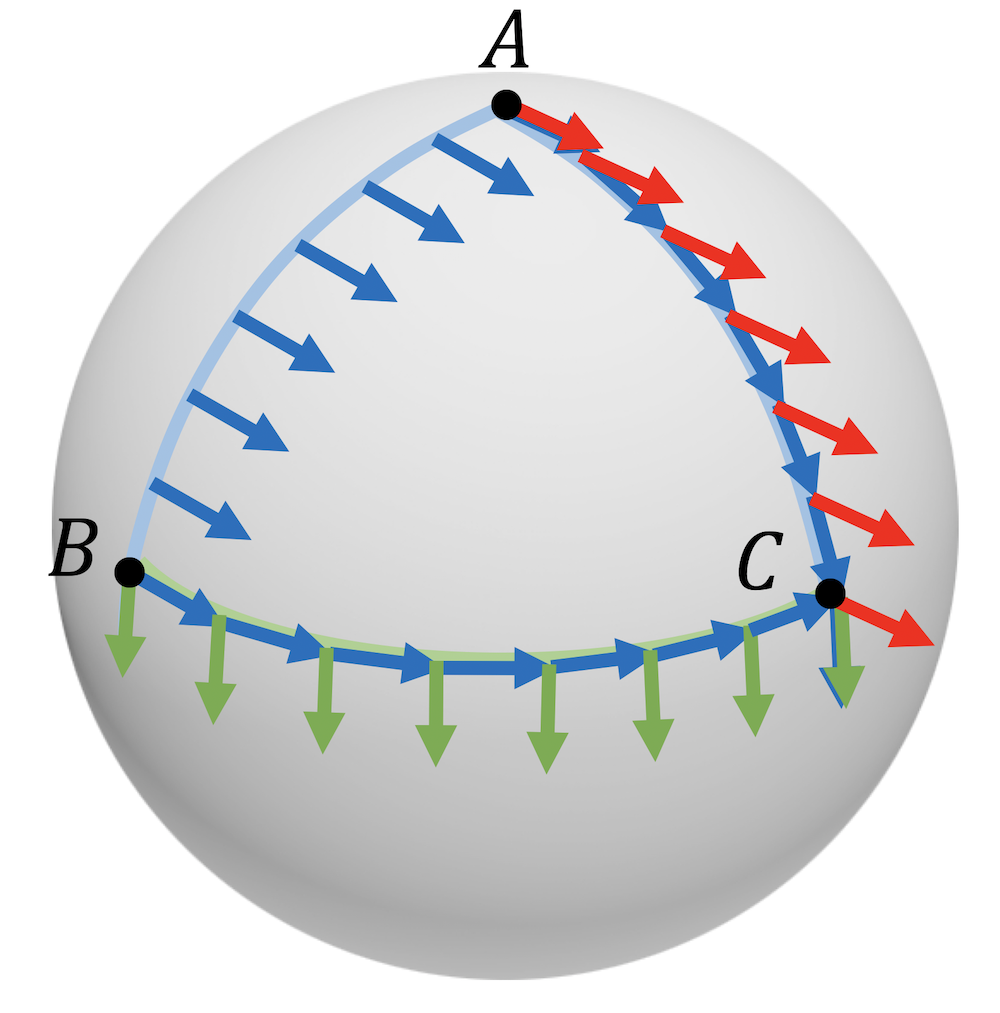
\includegraphics[width=0.9\linewidth]{figures/parallel.png}
Euclidean transport of a vector from A to C makes no sense on the sphere, as the resulting vectors (red) are not in the tangent plane. Parallel transport from A to C (blue) rotates the vector along the path. It is path dependent: going along the path BC and ABC produces different results.  
}
One issue we have already encountered when dealing with manifolds is that we cannot directly add or subtract two points $u,v \in \Omega$. 
%
The same problem arises when trying to compare tangent vectors at different points: though they have the same dimension, they belong to {\em different spaces}, e.g. $X\in T_u\Omega$ and $Y\in T_v\Omega$, and thus not directly comparable. 
%
Geodesics provide a mechanism to move vectors from one point to another, in the following way: let $\gamma$ be a geodesic connecting points $u=\gamma(0)$ and $v=\gamma(T)$ and let $X \in T_u\Omega$. We can define a new set of tangent vectors along the geodesic, $X(t) \in T_{\gamma(t)}\Omega$ such that the length of $X(t)$ and the angle (expressed through the Riemannian metric) between it and the velocity vector of the curve is constant,
$$
g_{\gamma(t)}(X(t),\gamma'(t) ) = g_{u}(X,\gamma'(0)) = \mathrm{const}, \quad\quad \|X(t)\|_{\gamma(t)} = \|X\|_u = \mathrm{const}.
$$
As a result, we get a unique vector $X(T) \in T_{v}\Omega$ at the end point $v$. %, which is unique. 


The map $\Gamma_{u\rightarrow v}(X) : T_u\Omega \rightarrow T_u\Omega$ and $T_v\Omega$ defined as $\Gamma_{u\rightarrow v}(X) = X(T)$ using the above notation is called {\em parallel transport} or {\em connection}; the latter term implying it is a mechanism to `connect' between the tangent spaces $T_u\Omega$ and $T_v\Omega$. 
%
Due to the angle and length preservation conditions, parallel transport amounts to only rotation of the vector, so it can be associated with an element of the special orthogonal group $\mathrm{SO}(s)$ (called the {\em structure group} of the tangent bundle),\marginnote{Assuming that the manifold is orientable, otherwise $\mathrm{O}(s)$.} which we will denote by $\fg_{u\rightarrow v}$ and 
discuss in further detail in Section~\ref{sec:gauges}. 

As we mentioned before,  a connection can be defined axiomatically independently of the Riemannian metric, providing thus an abstract notion of parallel transport along any smooth curve. The result of such transport, however, depends on the path taken.  
%As a general comment, parallel transport can be defined along any cur

%or {\em connection} 




\paragraph{Exponential map}
Locally around a point $u$, it is always possible to define a unique geodesic in a given direction $X \in T_u\Omega$, i.e. such that %a smooth curve $\gamma_X : [0,T] \rightarrow \Omega$ satisfying 
$\gamma(0) = u$ and $\gamma'(0) = X$. %, for some small $T>0$. 
%
%
When $\gamma_X(t)$ is defined for all $t\geq 0$ (that is, we can shoot the geodesic from a point $u$ for as long as we like), the manifold is said to be {\em geodesically complete} and the exponential map is defined on the whole tangent space.
%
Since compact manifolds are geodesically complete, we can tacitly assume this convenient property. 



%
This definition of geodesic provided a point and a direction gives a natural mapping from (a subset of) the tangent space $T_u \Omega$ to $\Omega$ called the {\em exponential map}\marginnote{
%Here, $B_\delta(0)$ is a ball of radius $\delta$ around the origin. 
Note that geodesic completeness does not necessarily guarantee that $\exp$ is a global diffeomorphism -- the largest radius $r$ about $u$ for which $\exp_u(B_r(0) \subseteq T_u\Omega)$ is mapped diffeomorphically is called the {\em injectivity radius}. }  $\exp : B_r(0) \subset T_u\Omega \rightarrow \Omega$, which is defined by taking a unit step along the geodesic in the direction $X$, i.e., $\exp_u(X) = \gamma_X(1)$. %
%
The exponential map $\exp_u$ is a local diffeomorphism, as it deforms the neighbourhood $B_r(0)$ (a ball or radius $r$) of the origin on $T_u\Omega$ into a neighbourhood of $u$. Conversely, one can also regard the exponential map as an intrinsic local deformation (`flattening') of the manifold into the tangent space. 




\paragraph{Geodesic distances}
%
A result known as the Hopf-Rinow Theorem 
%
\marginnote{Hopf-Rinow Theorem thus estabilishes the equivalence between geodesic and metric completeness, the latter meaning every Cauchy sequence converges in the geodesic distance metric.} guarantees that geodesically complete manifolds are also {\em complete metric spaces}, in which one can realise a distance (called the {\em geodesic distance} or {\em metric})  between any pair of points $u,v$ as the length of the shortest path between them
$$
d_g(u,v) = \min_{\gamma} \ell(\gamma) \quad\quad \text{s.t.} \quad\quad \gamma(0) = u, \,\, \gamma(T) = v,
$$
which exists (i.e., the minimum is attained).\marginnote{Note that the term `metric' is used in two senses: Riemannian metric $g$ and distance $d$. To avoid confusion, we will use the term `distance' referring to the latter. Our notation $d_g$ makes the distance depend on the Riemannian metric $g$, though the definition of geodesic length $L$. }



%The term `geodesic' is also used in metric geometry, where it is defined as the shortest path. In the setting described here the two meanings coincide. }


%i.e., the two notions of `geodesic' used somewhat differently in differential and metric geometry







\paragraph{Isometries}
Consider now a deformation of our manifold $\Omega$ into another manifold $\tilde{\Omega}$ with a Riemannian metric $h$, which we assume to be 
%
%We will assume this map to be 
a diffeomorphism $\eta: (\Omega, g) \rightarrow (\tilde{\Omega}, h)$ between the manifolds.   
%
Its differential $\mathrm{d}\eta : T\Omega \rightarrow T\tilde{\Omega}$ defines a map between the respective tangent bundles (referred to as {\em pushforward}), such that   
%\marginnote{The pushforward is what is called a {\em bundle map}.}
at a point $u$, we have $\mathrm{d}\eta_u : T_u \Omega \rightarrow T_{\eta(u)}\tilde{\Omega}$, %which allows to interpret it as follows: 
%
interpreted as before: 
if we make a small displacement from point $u$ by tangent vector $X \in T_u \Omega$, the map $\eta$ will be displaced from point $\eta(u)$ by tangent vector $\mathrm{d}\eta_u(X) \in T_{\eta(u)}\tilde{\Omega}$. 


Since the pushforward\marginnote{Pushforward and pullback are adjoint operators $\langle \eta^* \alpha, X \rangle = \langle \alpha, \eta_*X \rangle$ where $\alpha \in T^*\Omega$ is a {\em dual vector field}, defined at each point as a linear functional acting on $T_u\Omega$ and the inner products are defined respectively on vector and dual vector fields. } provides a mechanism to associate tangent vectors on the two manifolds, it allows to {\em pullback } the metric $h$ from $\tilde{\Omega}$ to $\Omega$, 
$$
(\eta^*h)_u(X,Y) = h_{\eta(u)}(\mathrm{d}\eta_u(X), \mathrm{d}\eta_u(Y))
$$ 
%
If the pullback metric coincides at every point with that of $\Omega$, i.e., $g = \eta^*h$, the map $\eta$ is called  (a Riemannian) {\em isometry}. % (metric-preserving). 
%
For two-dimensional manifolds (surfaces), isometries can be intuitively understood as inelastic deformations that deform the manifold without `stretching' or `tearing' it. 



By virtue of their definition, isometries preserve intrinsic structures such as geodesic distances, which are expressed entirely in terms of the Riemannian metric. % and Gaussian curvature.
%
Therefore, we can also understand isometries from the position of metric geometry, 
 as distance-preserving maps (`metric isometries') {\em between metric spaces} $\eta : (\Omega, d_g) \rightarrow (\tilde{\Omega}, d_h)$, in the sense that 
$$
d_g (u,v) = d_h(\eta(u),\eta(v)) 
$$
for all $u,v \in \Omega$, 
or more compactly, $d_g = d_h \circ (\eta \times \eta)$. In other words, Riemannian isometries are also metric isometries. 
%
On {\em connected} manifolds, the converse is also true: every metric isometry is also a Riemannian isometry. 
\marginnote{This result is known as the Myers–Steenrod Theorem. We tacitly assume our manifolds to be connected. }
%where $d_g, d_g$ are the geodesic distances induced by the respective Riemannian metrics $g, h$. 


In our Geometric Deep Learning blueprint, $\eta$ is a model of domain deformations. When $\eta$ is an isometry, %(roughly, an inelastic deformation that does not `stretch' the manifold), 
any intrinsic quantities are unaffected by such deformations. 
%
%This is the reason why we insist on working with structures defined intrinsically. 
%
One can generalise exact (metric) isometries through the notions of %this notion 
{\em metric dilation} 
$$
\mathrm{dil}(\eta) = \sup_{u\neq v \in \Omega}\frac{d_h(\eta(u),\eta(v))}{d_g (u,v)}
$$
%
or {\em metric distortion} 
$$
\mathrm{dis}(\eta) = \sup_{u, v \in \Omega}|d_h(\eta(u),\eta(v)) - d_g (u,v)|,
\marginnote{The Gromov-Hausdorff distance
%\marginnote{
%More precisely, $d_{\mathrm{GH}}(\Omega,\Omega') = \frac{1}{2}\inf_{(x,y) \in C} %\mathrm{dis}$
%} 
between metric spaces, which we mentioned in Section~\ref{sec:isomorphism}, can be expressed as the smallest possible metric distortion.}
$$
which capture the relative and absolute change of the geodesic distances under $\eta$, respectively. 
%
The condition~(\ref{eqn:domain_def_stability}) for the stability of a function $f \in \mathcal{F}(\mathcal{X}(\Omega))$ 
under domain deformation
can be rewritten in this case as 
$$
\| f(x,\Omega) - f(x\circ \eta^{-1},\tilde{\Omega})\| \leq C \|x\| \mathrm{dis}(\eta). 
$$


%[Gauss Theorema Egregium, definition of curvature through perimeter defect, pizza example]


\paragraph{Intrinsic symmetries}
A particular case of the above is a diffeomorphism  of the domain itself (what we termed {\em automorphism} in Section~\ref{sec:isomorphism}), which we will denote by $\tau \in \mathrm{Diff}(\Omega)$. We will call it a Riemannian  \mbox{(self-)isometry} if the pullback metric satisfies $\tau^* g = g$, or a metric (self-)isometry if $d_g = d_g\circ (\tau \times \tau)$.
%
Not surprisingly,\marginnote{Continuous symmetries on manifolds are infinitesimally generated by special tangent vector fields called {\em Killing fields}, named after Wilhelm Killing.} isometries form a group with the composition operator denoted by $\mathrm{Iso}(\Omega)$ and called the {\em isometry group}; the identity element is the map $\tau(u) = u$ and the inverse always exists (by definition of $\tau$ as a diffeomorphism). 
%
Self-isometries are thus {\em intrinsic symmetries} of manifolds.


%Continuous symmetries on manifolds are infinitesimally generated
%%\marginnote{More correctly, Killing fields are the infinitesimal generators of continuous symmetries. } 
%by special tangent vector fields called {\em Killing fields}, named after Wilhelm Killing. A field $X$ is Killing if the  Lie derivative\marginnote{The Lie derivative in this case is a derivative of forms. For scalar and vector fields, it coincides with the covariant derivative $\mathcal{L}_X y = \nabla_X y$ and the commutator $\mathcal{L}_X Y = [X,Y]$, respectively. } of the Riemannian metric along it vanishes, $\mathcal{L}_X g = 0$, which is interpreted as 
%%
%$$
%\mathcal{L}_X g(Y,Z) = g(\nabla_Y X, Z) + g(Y,\nabla_Z X) = 0
%$$
%for any smooth tangent fields $Y, Z$. 
%%
%We can recap that like we mentioned in Section~\ref{sec:symmetries}, we can regard symmetries as automorphisms (self-maps) preserving additional structure: either the local Riemannian metric, or global geodesic distances between pairs of points. 
%%\taco{Do we need Killing fields? It's interesting but I worry that we'd need to properly introduce Lie derivatives to make it understandable.} \michael{Lets keep them for now}
%%OK :)



\paragraph{Fourier analysis on Manifolds}
%Reconnecting to our Geometric Deep Learning blueprint, we now have a way to guarantee geometric stability by construction, considering intrinsic quantities expressed through the Riemannian metric. 
%
We will now show how to construct intrinsic convolution-like operations on manifolds, which, by construction, will be invariant to isometric deformations.    
For this purpose, 
%In order to define convolution-like operations, 
we have two options: One is to use an analogy of the Fourier transform, and define the convolution as a product in the Fourier domain. 
%
The other is to define the convolution spatially, by correlating a filter locally with the signal. 
%by ``shifting'' a filter around via parallel transport.
Let us discuss the spectral approach first.


We remind that in the Euclidean domain the Fourier transform is obtained as the eigenvectors of circulant matrices, which are jointly diagonalisable due to their commutativity. Thus, any circulant matrix and in particular, differential operator, can be used to define an analogy of the Fourier transform on general domains. 
%
In Riemannian geometry, it is common to use the orthogonal eigenbasis of the Laplacian operator, which we will define here. 


For this purpose, recall our definition of the intrinsic gradient operator $\nabla : \mathcal{X}(\Omega,\mathbb{R}) \rightarrow \mathcal{X}(\Omega,T\Omega)$, 
%assigning at each point $x(u) \mapsto \nabla x(u) \in T_u \Omega$. In other words, the gradient produces 
producing a tangent vector field that indicates the local direction of steepest increase of a scalar field on the manifold. 
%
In a similar manner, we can define the {\em divergence operator} $\nabla^* : \mathcal{X}(\Omega,T\Omega) \rightarrow \mathcal{X}(\Omega,\mathbb{R})$. 
%
If we think of a tangent vector field as a
flow on the manifold, the divergence measures
the net flow of a field at a point, allowing to distinguish
between field `sources' and `sinks'. 
%
We use the notation $\nabla^*$ (as opposed to the common $\mathrm{div}$) to emphasise that the two operators are adjoint,
$$
\langle X, \nabla x\rangle = \langle \nabla^* X,  x\rangle,
$$
where we use the inner products (\ref{eq:inner_scalar}) and~(\ref{eq:inner_vector}) between scalar and vector fields. 
%with the inner products defined on vector and scalar fields, respectively. 

The {\em Laplacian} (also known as the {\em Laplace-Beltrami operator} in differential geometry) is an operator on $\mathcal{X}(\Omega)$ defined as $\Delta = \nabla^* \nabla$,  
%; as opposed to most of the textbooks, we use the negative sign to ensure our operator is positive semi-definite. 
%
which can be interpreted \marginnote{From this interpretation it is also clear that the Laplacian is isotropic. We will see in Section~\ref{sec:meshes} that it is possible to define {\em anisotropic Laplacians} (see \citep{andreux2014anisotropic,boscaini2016anisotropic}) of the form $\nabla^*(A(u)\nabla)$, where $A(u)$ is a position-dependent tensor determining local direction. 
%In practice, such a construction requires a fixed gauge. 
}
%For the classical Euclidean Laplacian defined as the sum of second-order derivatives this can be seen by writing it as the trace of the Hessian, $\Delta x(\mathbf{u})= \mathrm{trace} \nabla^2 x(\mathbf{u})$, applying an orthogonal transformation of coordinates $\mathbf{u}\mapsto \mathbf{Ru}$,  and using the chain rule.
%}
as the difference between the average of a function on an
infinitesimal sphere around a point and the value of the
function at the point itself. 
%
%
It is one of the most important operators in mathematical physics, used to describe phenomena as diverse as heat diffusion, quantum oscillations,
and wave propagation.  
%
Importantly in our context, the Laplacian is intrinsic, and thus invariant under isometries of $\Omega$. 



It is easy to see that the Laplacian is self-adjoint (`symmetric'),
$$
\langle \nabla x, \nabla x \rangle = \langle x , \Delta x\rangle = \langle \Delta x ,  x\rangle.
$$
The quadratic form on the left in the above expression is actually the already familiar Dirichlet energy,  
$$c^2(x) = \| \nabla x \|^2 = \langle \nabla x, \nabla x \rangle = \int_\Omega \| \nabla x(u) \|_u^2 \mathrm{d}u = \int_\Omega g_u( \nabla x(u),  \nabla x(u)) \mathrm{d}u
$$
measuring the smoothness of $x$. 
%As we will see in the following, the Laplacian plays a center role in signal processing and learning on non-Euclidean domains, as its eigenfunctions generalize the classical Fourier bases, allowing to perform spectral analysis on manifolds and graphs
%
%
%
%
%allowing to interpret it as the smoothest orthogonal basis. 
%
%
%We will discuss this construction in detail in Chapter ???, where we will show that Laplacian eigenvalues and eigenvectors capture important geometric properties of the manifold. 



The Laplacian operator admits an eigedecomposition %eigenfunctions
$$
\Delta \varphi_k = \lambda_k \varphi_k, \quad\quad k=0, 1, \hdots 
$$
%
%which is discrete 
with countable spectrum if the manifold is compact (which we tacitly assume), and orthogonal eigenfunctions, $\langle \varphi_k, \varphi_l \rangle = \delta_{kl}$, due to the self-adjointness of $\Delta$. 
%discrete on compact manifolds
%orthogonal since $\Delta$ is self-adjoint
%
The Laplacian eigenbasis can also be constructed as a set of orthogonal minimisers of the Dirichlet energy, 
$$
\varphi_{k+1} = \arg\min_{\varphi} \| \nabla \varphi \|^2      \quad\quad \text{s.t.}\quad\quad   \|\varphi \|=1 \,\,\, \text{and} \,\,\, \langle \varphi, \varphi_{j} \rangle = 0 
$$
for $j=0,\hdots, k$, allowing to interpret it as the smoothest orthogonal basis on $\Omega$. 
%
The eigenfunctions $\varphi_0, \varphi_1, \hdots$ and the corresponding eigenvalues $0 = \lambda_0 \leq \lambda_1 \leq \hdots $ can be interpreted as the analogy of the atoms and frequencies in the classical Fourier transform. \marginnote{In fact $e^{\mi \xi u}$ are the eigenfunctions of the Euclidean Laplacian $\tfrac{\mathrm{d}^2}{\mathrm{d} u^2}$.}
%


This orthogonal basis allows to expand square-integrable functions on $\Omega$ into {\em Fourier series}  
$$
x (u) = \sum_{k \geq 0} \langle x, \varphi_k \rangle \varphi_k (u)
$$
%
where $\hat{x}_k = \langle x, \varphi_k \rangle$ are referred to as the {\em Fourier coefficient} or the (generalised) Fourier transform of $x$. \marginnote{Note that this Fourier transform has a discrete index, since the spectrum is discrete due to the compactness of $\Omega$.}
%
Truncating the Fourier series results in an approximation error that can be bounded \citep{aflalo2013spectral} by 
$$
\left\| x - \sum_{k = 0}^N \langle x, \varphi_k \rangle \varphi_k \right\|^2 \leq \frac{\| \nabla x\|^2}{\lambda_{N+1}}.
$$
\cite{aflalo2015optimality} further showed that no other basis attains a better error, making the Laplacian eigenbasis  {\em optimal} for representing smooth signals on manifolds. 


\paragraph{Spectral Convolution on Manifolds}
%Let us now remind the reader that we defined Euclidean convolution in Section~\ref{sec:groups} as inner product with a shifted filter $(x \star \psi)(u) =  \langle x, T_u \psi \rangle$. This construction had two important properties, linearity and commutativity, that works in both ways, allowing to {\em define} convolution as a linear operator that commutes with shift. 
%%
%On a manifold, because we lack a global vector space structure, we cannot immediately define the shift operator $(T_v x)(u) = x(u-v)$ since ``$u-v$'' makes no sense. 
%%
%However, we can keep $T_u$ as an abstract linear operator and use the above two properties as a definition. 
%
%
%First, we note that commutativity implies 
%$$
%(T_v (x\star \psi))(u) = \langle x, T_v T_u \psi \rangle =  \langle T_v x, T_u  \psi \rangle = ((T_v x)\star \psi)(u).  
%$$
%%
%Expressing each of the functions %$x$, $T_u \psi$, and $T_v x$ 
%in the Fourier basis allows us to rewrite %this identity as 
%\begin{eqnarray*}
%\langle T_v x, T_u\psi \rangle &=& \left \langle 
%\sum_{k\geq 0} \langle T_v x,\varphi_k \rangle \varphi_k \,, \,\,
%\sum_{l\geq 0} \langle T_u\psi,\varphi_l \rangle \varphi_l
%\right \rangle \\
%&=& \sum_{k,l\geq 0} \langle T_v x,\varphi_k \rangle \langle T_u\psi,\varphi_l \rangle \langle \varphi_k, \varphi_l \rangle \\
%&=& \sum_{k \geq 0} \langle T_v x,\varphi_k \rangle \langle T_u\psi,\varphi_k \rangle, \marginnote{We use here the orthogonality of the basis, $\langle \varphi_k, \varphi_l \rangle = \delta_{kl}$.}
%\end{eqnarray*}
%%
%and similarly, 
%$
%\langle x, T_v T_u\psi \rangle =
%\sum_{k \geq 0} \langle x,\varphi_k \rangle \langle T_v  T_u\psi,\varphi_k \rangle
%$,
%%
%from where the spectral expression of the commutativity condition follows:
%$$
%\langle T_v x,\varphi_k \rangle \langle T_u\psi,\varphi_k \rangle 
%= \langle x,\varphi_k \rangle \langle T_v  T_u\psi,\varphi_k \rangle \quad\quad \text{for all} \, k\geq 0.
%$$
%In particular, for $x=\psi = \varphi_l$ we get 
%$
%\langle T_v \varphi_l,\varphi_k \rangle \langle T_u \varphi_l,\varphi_k \rangle 
%= \delta_{kl} \langle T_v  T_u \varphi_l,\varphi_k \rangle 
%$
%which leads us to $\langle T_v \varphi_l,\varphi_k \rangle = 0$ for $k\neq l$. This means that Fourier basis functions are the eigenfunctions of the shift operator, like we had in the Euclidean case,  i.e., $T_v \varphi_k = \mu_v \varphi_k$.
%
%
%In order to determine the eigenvalues $\mu_v$, we consider again the commutativity condition with $x=\varphi_k$ and $\psi = \delta_u$ the Dirac delta function\marginnote{The {\em Dirac delta} or {\em impulse function} is defined as $\langle \delta_u , x \rangle = x(u)$. It can thus be considered as the representation of the linear functional (dual vector) $x \mapsto x(u)$.  } 
%
%
%
%Second, using  the linearity of $T_v$, we get 
%%the general expression  
%$$
%(T_v x)(u) = \sum_{k\geq 0} \langle x, \varphi_k\rangle (T_v \varphi_k) (u)
%= \sum_{k\geq 0} \langle x, \varphi_k\rangle  \varphi_k (v) \varphi_k (u)
%= \sum_{k\geq 0} \hat{x}_k  \varphi_k (v) \varphi_k (u), 
%%\marginnote{In the Euclidean case, one has (from the associativity of exponents and complex conjugation in the inner product) $\varphi_i (v) \bar{\varphi}_i (u) = \varphi_i (v - u)$. In the general case, the shift operator is thus position-dependent and the signal is {\em changed} when shifted.  }
%$$
%which is a non-Euclidean generalisation of the shift operator. 
%%
%It is easy to verify that in the Euclidean case, $\Omega = [0,L]$, \marginnote{ Here we assume a compact interval, in which case the Fourier basis is discrete. Note that the shift we get is $x(u+v)$ rather than $x(u-v)$, which is just notational difference.}  where the Fourier basis is of the form $\varphi_k(u) = e^{\mi \frac{2\pi k}{L} u}$, we get the familiar expression 
%$$
%(T_v x)(u) = \sum_{k\geq 0} \hat{x}_k e^{\mi \frac{2\pi k}{L} v} e^{\mi \frac{2\pi k}{L} u} 
%\sum_{k\geq 0} \hat{x}_k e^{\mi \frac{2\pi k}{L} (u+v)} = x(u+v).
%$$
%
%
%Finally, plugging the expression of $T_u$ into the definition of convolution, we get
%%{\em spectral convolution}
%%
%\begin{eqnarray}
%(x \star \psi)(u) &=& \langle x, T_u \psi \rangle = 
%\left \langle x, \, \sum_{k\geq 0} \hat{\psi}_k \varphi_k(u) \phi_k 
%\right\rangle \nonumber \\
%&=&
%\sum_{k \geq 0} \langle x, \varphi_k \rangle \hat{\psi}_k  \varphi_k (u)  = \sum_{k \geq 0} (\hat{x}_k \cdot \hat{\psi}_k ) \varphi_k (u).
%\label{eqn:conv_spectral}
%\end{eqnarray}
%%
%%In a sense, we used what was a {\em property} of the classical Fourier transform (the Convolution Theorem) as a way to {\em define} a non-Euclidean convolution. 
%%
%Expression~(\ref{eqn:conv_spectral}) is often called {\em spectral convolution}, since it coincides with the Convolution Theorem, expressing the convolution in spectral domain as the point-wise product of the Fourier transforms $\hat{\psi}_k$ and $\hat{x}_k$.  
%%
%This construction is usually motivated by using a {\em property} of the classical Fourier transform (the Convolution Theorem) as a way to {\em define} a non-Euclidean convolution. However, here we have shown the derivation from first principles of shift equivariance (where the shift is understood in a more general sense). 
%%
%The key property of spectral convolution is that, by virtue of its construction, it is intrinsic and thus isometry-invariant. 




{\em Spectral convolution} can be defined as the product of Fourier transforms of the signal $x$ and the filter $\theta$, 
\begin{equation}
(x \star \theta)(u) = 
\sum_{k \geq 0} (\hat{x}_k \cdot \hat{\theta}_k ) \varphi_k (u).
\label{eqn:conv_spectral}
\end{equation}
%
Note that here we use what is a {\em property} of the classical Fourier transform (the Convolution Theorem) as a way to {\em define} a non-Euclidean convolution.
%
By virtue of its construction, the spectral convolution is intrinsic and thus isometry-invariant. 
%
Furthermore, since the Laplacian operator is isotropic, it has no sense of direction; in this sense, the situation is similar to that we had on graphs in Section~\ref{sec:proto-graphs} due to permutation invariance of neighbour aggregation. 







\begin{figure}[h!]
    \centering
    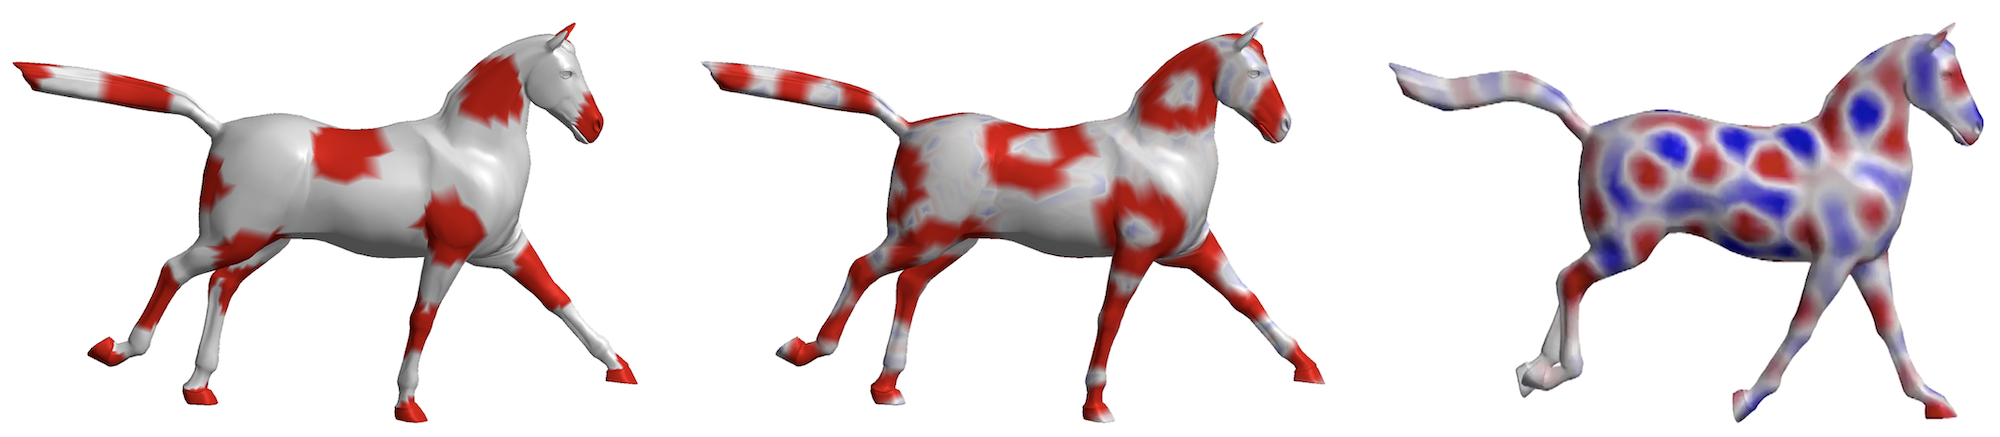
\includegraphics[width=\linewidth]{figures/horses.png}
    \caption{Instability of spectral filters under domain perturbation. Left: a signal $\mathbf{x}$ on the mesh $\Omega$. Middle: result of spectral filtering %$\mathbf{x}\star \boldsymbol{\theta} = \boldsymbol{\Phi}\, \mathrm{diag}(\hat{\boldsymbol{\theta}}) \boldsymbol{\Phi}^\top \mathbf{x}$ 
    in the eigenbasis %$\boldsymbol{\Phi}$ 
    of the Laplacian $\Delta$ on $\Omega$. 
    Right: 
    the same spectral filter %$\boldsymbol{\theta}$ 
    applied to the eigenvectors %$\bar{\boldsymbol{\Phi}}$ 
    of the Laplacian $\tilde{\Delta}$ of a nearly-isometrically perturbed domain $\tilde{\Omega}$ 
    %(as a result of a near-isometric deformation of the mesh)  
%    $\bar{\boldsymbol{\Phi}}\, \mathrm{diag}(\hat{\boldsymbol{\theta}}) \bar{\boldsymbol{\Phi}}^\top \mathbf{x}$
    produces a very different result. 
    }
    \label{fig:mesh_horses}
\end{figure}%




%
In practice, a direct computation of~(\ref{eqn:conv_spectral}) appears to be prohibitively expensive due to the need to diagonalise the Laplacian. Even worse, 
%, as we will see in Section~\ref{sec:meshes}, 
it turns out geometrically unstable: the higher-frequency eigenfunctions of the Laplacian can change dramatically as a result of even small near-isometric perturbations of the domain $\Omega$ (see Figure~\ref{fig:mesh_horses}). 
%
%
A more stable solution is provided by realising the filter as a {\em spectral transfer function} of the form $\hat{p}(\Delta)$, 
%which is understood in the operator sense as %\marginnote{Geometric Deep Learning methods based on spectral convolution expressed through the Fourier transform are often referred to as `spectral' and opposed to `spatial' methods we have seen before in the context of graphs. When expressed as spectral transfer function, the former in fact boil down to the latter, so this dichotomy is somewhat artificial and not completely appropriate.}
\begin{eqnarray}
(\hat{p}(\Delta) x)(u) &=& \sum_{k\geq 0} \hat{p}(\lambda_k) \langle x, \varphi_k\rangle \varphi_k (u) \label{eqn:conv_spec} \\
%
&=& \int_\Omega x(v) \, \sum_{k\geq 0} \hat{p}(\lambda_k) \varphi_k(v) \varphi_k (u) \, \mathrm{d}v \label{eqn:conv_spat}
\end{eqnarray}
%
which can be interpreted in two manners: either as a spectral filter~(\ref{eqn:conv_spec}), where we identify $\hat{\theta}_k = \hat{p}(\lambda_k)$, or as a spatial filter~(\ref{eqn:conv_spat}) with a position-dependent kernel $\theta(u,v) = \sum_{k\geq 0} \hat{p}(\lambda_k) \varphi_k(v) \varphi_k (u)$.  
%
%
The advantage of this formulation is that $\hat{p}(\lambda)$ can be parametrised by a small number of coefficients, and choosing parametric functions such as polynomials\marginnote{Geometric Deep Learning methods based on spectral convolution expressed through the Fourier transform are often referred to as `spectral' and opposed to `spatial' methods we have seen before in the context of graphs. We see here that these two views may be equivalent, so this dichotomy is somewhat artificial and not completely appropriate.} $\hat{p}(\lambda) = \sum_{l=0}^r \alpha_l \lambda^l$ allows for efficiently computing the filter as 
$$
(\hat{p}(\Delta) x)(u) = \sum_{k\geq 0} \sum_{l= 0}^r \alpha_l \lambda_k^l \, \langle x, \varphi_k\rangle \varphi_k (u) = \sum_{l= 0}^r \alpha_l (\Delta^l x)(u),
$$
avoiding the spectral decomposition altogether. 
%
We will discuss this construction in further detail in Section~\ref{sec:meshes}. 

%\michael{Add note on stability}

%While filters defined in this manner are isotropic (direction-unaware), 



\paragraph{Spatial Convolution on Manifolds}

A second alternative is to attempt defining convolution on manifolds is by matching a filter at different points, like we did in formula~(\ref{eq:group-conv}), 
%
\begin{equation}
(x \star \theta)(u) = \int_{T_u \Omega} x(\exp_u Y) \theta_u(Y) \mathrm{d}Y, 
\label{eq:conv_tangent_space}
\end{equation}
%
where we now have to use the exponential map to access the values of the scalar field $x$ from the tangent space, and 
the filter $\theta_u$ is defined in the tangent space at each point and hence position-dependent. %
If one defines the filter intrinsically, such a convolution would be isometry-invariant, a property we mentioned as crucial in many computer vision and graphics applications. 
%, and we use the exponential map to obtain. 


We need, however, to note several substantial differences from our previous construction in Sections~\ref{sec:grids_euclidean}--\ref{sec:groups}. 
%
First, because a manifold is generally not a homogeneous space, we do not have anymore a global group structure allowing us have a shared filter (i.e., the same $\theta$ at every $u$ rather than $\theta_u$ in expression~(\ref{eq:conv_tangent_space})) defined at one point and then move it around. 
%as we did in formula~(\ref{eq:group-conv}). 
%
An analogy of this operation on the manifold would require parallel transport, allowing to apply a shared $\theta$, defined as a function on $T_u\Omega$, at some other $T_v\Omega$.   
%
However, as we have seen, this in general will depend on the path between $u$ and $v$, so {\em the way we move the filter around matters.}%\marginnote{As a possible remedy, \cite{poulenard2018multi} suggested moving the filter along geodesics. } 
%
%
Third, since we can use the exponential map only locally, the filter must be {\em local}, with support bounded by the injectivity radius.  
%
Fourth 
and most crucially, we cannot work with $\theta(X)$, as $X$ is an abstract geometric object: in order for it to be used for computations, we must represent it {\em relative to some local basis}  
$\omega_u : \mathbb{R}^s \rightarrow T_u\Omega$, as an $s$-dimensional array of coordinates $\mathbf{x} = \omega^{-1}_u(X)$. 
%
This allows us to rewrite the convolution~(\ref{eq:conv_tangent_space}) as 
%
\begin{equation}
(x \star \theta)(u) = \int_{[0,1]^s} x(\exp_u (\omega_u \mathbf{y})) \theta(\mathbf{y}) \mathrm{d}\mathbf{y}, 
\label{eqn:conv_exp}
\end{equation}
%

%\joan{We have used $\delta$ in the previous sections to refer to the size of the filter support}

with the filter defined on the unit cube. Since the exponential map is intrinsic (through the definition of geodesic), the resulting convolution is isometry-invariant. 


Yet, this tacitly assumed  we can carry the frame $\omega_u$ along to another manifold, i.e. $\omega_u' = \mathrm{d}\eta_u \circ \omega_u$.
%
%Yet, we should point to one issue that at a close inspection opens a can of worms: in our definition, we assumed $\omega$ was given, which 
Obtaining
such a frame (or \emph{gauge}, in physics terminology) given only a the manifold $\Omega$ in a consistent manner is however fraught with difficulty.
%implies that we need some mechanism to {\em fix a basis at each point} of the manifold (in physics, a smooth choice of local bases is referred to as a {\em gauge}). 
%
First, a smooth global gauge may not exist: this is the situation on manifolds that are not \emph{parallelisable},\marginnote{The sphere $\mathbb{S}^2$ is an example of a non-parallelisable manifold, a result of    
%on which one cannot construct a smooth tangent vector field. 
the {\em Poincar{\'e}-Hopf Theorem}, which is colloquially stated as `one cannot comb a hairy ball without creating a cowlick.' \vspace{2mm}
%and is the reason why magnetic plasma confinement chambers must have toroidal rather than spherical geometry. 
%\includegraphics[width=1\linewidth]{figures/hairy_ball.png}
}   in which case one cannot define a smooth non-vanishing tangent vector field.
%; we further assume that the global gauge is smooth, which is only possible if the manifold is {\em parallelizable}.
%
%
Second, we do not have a canonical gauge on manifolds, so this choice is arbitrary; since our convolution depends on $\omega$, if one chose a different one, we would obtain different results. 

We should note that this is a case where practice diverges from theory: in practice, 
%one can get around these mathematical issues in a somewhat satisfactory manner.
%That is, 
%there exist algorithms that will 
it is possible to build frames that are mostly smooth, with a limited number of singularities, e.g. by taking the intrinsic gradient of some intrinsic scalar field on the manifold.  \marginnote{
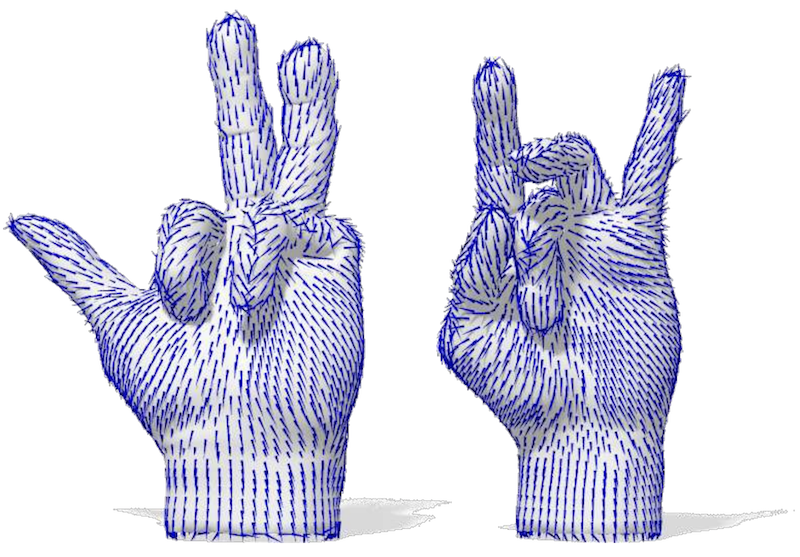
\includegraphics[width=1\linewidth]{figures/gframes.png} 
Example of stable gauges constructed on nearly-isometric manifolds (only one axis is shown) using the GFrames algorithm of \cite{melzi2019gframes}.
} 
%(such as e.g. the North and South pole of the sphere in the sidebar), for instance taking the two frame vectors to correspond to the highest and least curved direction on a 2D manifold. 
%
Moreover, such constructions are stable, i.e., the frames constructed this way will be identical on isometric manifolds and similar on approximately isometric ones. 
%
Such approaches were in fact employed in the early works on deep learning on manifolds  \citep{masci2015geodesic,monti2017geometric}.
%the same frame is found for isometric manifolds, and for nearly isometric ones a similar frame is found. 


Nevertheless, this solution is not entirely satisfactory because near singularities, the filter orientation (being defined in a fixed manner relative to the gauge) will vary wildly, leading to a non-smooth feature map even if the input signal and filter are smooth. 
%
Moreover, there is no clear reason why a given direction at some point $u$ should be considered equivalent to another direction at an altogether different point $v$. 
%
Thus, despite {\em practical} alternatives, we will look next for 
%methods based on semi-intrinsic frames can be useful, 
a more {\em theoretically} well-founded approach that would be altogether independent on the choice of gauge. 
%which we will discuss next. 
%We will discuss just such an approach next.


%\joan{This is still a bit long, but already much improved from earlier versions. 
%One aspect that is still not very explicit is how to precisely connect with the GDL blueprint, in terms of the composition of local equivariant maps, and global invariant map. 
%Here we argue that differential operators such as the Laplacian are defined intrinsically (isometry invariant), and thus any representation that is based on it will preserve this isometric invariance. Equivariance in this context is less obvious (equivariance with respect to changes in the gauge, parametrisation/charting?).

%Also, should we mention stability of the Laplacian to metric deformations? How to ensure that the information we extract from the Laplacian is not too unstable? we can mimic the discussion from previous section on wavelet vs fourier, to illustrate that the high-frequency eigenfunctions of the laplace-beltrami  are unstable. THis is mentioned in the mesh section, should it be restated here as well?
%}

%
%
%Assume now we have some vector-valued data $\Omega$. 
%In differential geometry, this is modelled as a {\em vector field} $x:\Omega \rightarrow T\Omega$, assigning to each point $u \in \Omega$ a tangent vector $x(u) \in T_u \Omega$. 
%%
%%
%%The reason we need to consider gauges is that we can only describe geometric data numerically \emph{relative to a gauge}.
%%
%Relative to a gauge, we can express each tangent vector as a coordinate vector, i.e. an array of numbers, and so a vector field becomes a map $\mathbf{x} : \Omega \rightarrow \R^{s}$.
%%
%In other words, we can, as previously, think of vector fields as signals forming the space $\mathcal{X}_{\R^s}(\Omega)$ with the inner product 
%%(\ref{eqn:innerprod}) [Only well defined if we choose a metric? Should we assume Riemannian manifolds?]. 
%$$
%\langle x, y\rangle = 
%\int_\Omega  \langle x(u), y(u) \rangle_{T_u\Omega} du = 
%\int_\Omega \mathbf{x}^\top(u) \mathbf{G}(u) \mathbf{y}(u) du,  
%$$
%%
%where $\mathbf{G}$ is the representation of the {\em Riemannian metric} (defined as an inner product on $T_u\Omega$ depending smoothly on $u$) in the same local frame.
%%

%As in the examples discussed in previous sections, this group can act via different representation $\rho$, which in this case corresponds to different kinds of fields, including scalar fields, vector fields, tensor fields, each of which is characterized by how it transforms under a change of gauge.



%\paragraph{Local Symmetries and Spatial Weight Sharing}


% ----
% OLD:

% Let us start from the simplest case of {\em scalar fields}, i.e. signals $\mathcal{X}(\Omega, \mathbb{R})$. 
% %




% Importantly, not only the {\em features} change when we change the gauge, also the {\em network layers} depend on the choice of gauge. 
% %
% Consider an architecture in the spirit of `message passing' we saw in graph neural networks, where at each point $u\in \Omega$, we aggregate the transformed feature vectors from neighbor points $v$, 
% and 
% %
% for simplicity, assume this transformation is linear. 
% %
% When the vectors are expressed w.r.t. a gauge, this transformation takes the form of matrix multiplication  $\mathbf{A}(u,v)\mathbf{x}(v)$; this notation emphasizes the fact that the matrix can be different for each pair of points $u, v$.  
% %.\marginnote{What we describe here is the GCN architecture. In attentional architectures, we can have $\mathbf{A}(\mathbf{x}(u),\mathbf{x}(u'))$ rather than $\mathbf{A}(u, u')$. }
% %
% %Note however an crucial difference: on a graph, the matrix $\mathbf{A}$ must be {\em the same} for all points $u'$, as this is needed for permutation equivariance. 
% %
% %In the case of a manifold, there is no such a global symmetry, so we can use a different matrix $\mathbf{A}(u,u')$ for each pair of (neighbor) points. 



% If we perform a gauge transformation, the input feature vector changes as $\mathbf{x}(u) \mapsto \rho(\fg(u)) \mathbf{x}(u)$, and the output feature should change as $\mathbf{x}(v) \mapsto \rho(\fg(v)) \mathbf{x}(v)$\marginnote{We assume here for simplicity that the input and output features are of the same type and thus have the same representation $\rho(\fG)$.}.
% It follows that we should change $\mathbf{A}(u,v) \mapsto \rho(\fg(v)) \mathbf{A}(u,v) \rho(\fg(u))^{-1}$.
% Although the new weight matrix and feature vectors contain different numbers, the underlying geometric objects are mapped in the same way regardless of the gauge.



% % Gauge equivariant message; 
% If gauge transformations are considered as symmetries, a network layer, and hence an individual message, should be equivariant to gauge transformations.
% That is, the weight matrix $A_{uu'}$ should satisfy $\rho(g(u'))^{-1} A_{uu'} = A_{uu'} \rho(g(u))$ for all gauge transformations $g : \Omega \rightarrow \fG$.
% This is an extremely strong constraint, because $g(u)$ and $g(u')$ (the gauge transformation at $u$ and $u'$) can vary independently.
% As a consequence the weight matrix $A_{uu'}$ is so constrained that it cannot learn very interesting mappings.

% % Connection
% The solution is to introduce an additional piece of structure called a \emph{connection}, which relates the feature spaces at $u$ and $u'$. % via parallel transport (see Figure TODO).
% The connection gives us for any two nearby points $u, u'$ a straightest curve (geodesic) between them, and a notion of \emph{parallel transport} of frames and feature vectors along this curve (see Figure TODO).
% %The parallel transporter from $u$ to $u'$ along a geodesic is an element of $\fG$ denoted $\fg_{u \rightarrow u'} \in \fG$ that transforms as $\fg_{u \rightarrow u'} \mapsto \fg(u') \fg_{u \rightarrow u'} \fg(u)^{-1}$ under a gauge transformation $\fg(u)$.
% Using parallel transport, we can move the feature vector $v_u$ at $u$ to $u'$, before applying the weight matrix $A_{uu'}$.
% Since this matrix maps input features at $u$ to output features at $u$, it only has to deal with the gauge at $u$.
% In other words, it should satisfy a more conventional equivariance constraint: $A_{uu'} \rho(g(u)) = \rho(g(u)) A_{uu'}$ that only involves $g(u)$ and not $g(u')$. \michael{[TACO: isn't it the other way around, you transport vectors from u' to u?]}

% % Spatial weight sharing; filter on tangent plane; identify tangent planes via gauge;
% What we have seen so far is that gauge symmetries constrain the weight matrix $A_{uu'}$, but that the weight matrices associated with different points need not necessarily share weights as in a convolution layer.




%In each of the examples discussed so far, we started with a space $\Omega$ and a group of symmetries $\fG$ acting on it.
%In some cases however, e.g. when the domain $\Omega$ is a general manifold or mesh, it may not have any obvious symmetries.
%%For instance, if $\Omega$ is a general manifold, it may not have any non-trivial symmetries.
%In this case, we cannot define an action of $\fG$ on the space of signals on $\Omega$ and use it to slide filters around to define a convolution.
%Nevertheless, in this example as many others, there is still a group of symmetries lurking beneath the surface, but this is an altogether kind of symmetry known as \emph{gauge symmetry}.
%
%The word gauge here refers to a choice of frame (ordered basis) for a vector space, or more generally to one such choice for each vector space in a collection of vector spaces $V_u$ associated with the points $u \in \Omega$.
%For example, if we have a manifold $\Omega$, we can construct the \emph{tangent bundle} $T \Omega$ which consists of a collection of vector spaces $T_u \Omega$ (the tangent spaces), one for each point in $u \in \Omega$ (see Figure TODO).
%So in this example a gauge is a choice of frame for each of the tangent spaces $T_u \Omega$.\marginnote{
%We note that in mathematical gauge theory one would require the gauge to be smooth, in which case a globally defined gauge may not always exist. We will ignore these subtleties and not insist on smoothness.
%}
%
%The reason we need to consider gauges is that we can only describe geometric data numerically \emph{relative to a gauge}.
%Let's imagine our data consists of a vector field on $\Omega$.
%A vector field assigns to each point $u \in \Omega$ a tangent vector $v \in T_u \Omega$.
%Relative to a gauge, we can express each tangent vector as a coordinate vector, i.e. a list of numbers, and so a vector field becomes a map $x : \Omega \rightarrow \R^{n}$ (where $n$ is the dimension of the manifold and tangent spaces).
%In other words, our input space is $\mathcal{X}(\Omega, \R^n)$.
%However it is important to realize that what we are really interested in is the underlying geometrical object (vector field), whose representation as a function $x \in \mathcal{X}(\Omega, \R^n)$ depends on the choice of gauge.
%%However there is no canonical choice of gauge, so depending on our choice we will get different coordinate vectors.
%
%When we change the gauge, there is at each position a unique invertible matrix that maps the old gauge to the new one.
%In other words, a gauge transformation is a mapping $g : \Omega \rightarrow \GL{n}$, where $\GL{n}$ is the group of invertible $n \times n$ matrices.
%We can also restrict our attention to e.g. right-handed orthogonal frames, which are related by rotations, in which case a gauge transformation is a map $g : \Omega \rightarrow \SO{n}$ assigning to each position a rotation.
%In general, one considers a group $\fG$ (called the structure group) and a collection of frames such that for any two of them there is a unique $\fg \in \fG$ that maps one frame onto the other.
%As in the examples discussed in previous sections, this group can act via different representation $\rho$, which in this case corresponds to different kinds of fields, including scalar fields, vector fields, tensor fields, each of which is characterized by how it transforms under a change of gauge.
%
%% Associated bundles / reps of G
%% In the previous sections on Graphs, Grids and Groups, we discussed how the same group may act on various feature spaces through different representations $\rho$.
%% In the case of gauge transformations the same is true: we can define various kinds of fields such as scalar, vector, and tensor fields, by choosing an appropriate representation $\rho$ of the structure group $\fG$.
%% For instance, a scalar field (e.g. surface temperature on earth) does not depend on the frame (a scalar does not have a direction), so it corresponds to the trivial representation $\rho_0(g) = 1$.
%% A 2-tensor field would transform as $A_u \mapsto \fg A_u \fg^T$, where $u \in \Omega$, $A_u \in \R^{n \times n}$ and $\fg \in \fG$ is the change of basis matrix relating two gauges.
%
%%Given two vector fields, we can take at each position the outer (tensor) product $v w^T$ to obtain a tensor field, which tra
%
%% Gauge equivariant message from u to v; need for a connection / parallel transport
%%If gauge transformations are considered as symmetries, a network layer should be equivariant to gauge transformations.
%Not only the features change when we change the gauge, also the network layers depend on the choice of gauge.
%We will consider a message passing layer, and focus first on a single message sent from $u \in \Omega$ to $u' \in \Omega$.
%In a graph neural network, one would take the feature vector $v_u$ at $u$ and multiply it by a weight matrix $A$ to get the feature vector $v_{u'}$ at $u'$, before summing over all neighbours $u'$.
%The same weight matrix is used for all pairs of adjacent points $u,u'$, because this is required for equivariance to permutations.
%In the case of a manifold, we don't have such a global symmetry, so we are free to use a different matrix $A_{uu'}$ for each pair of (nearby) points $u, u'$.
%Now if we perform a gauge transformation, the input feature changes as $v_u \mapsto \rho(g(u)) v_u$, and the output feature should change as $v_{u'} \mapsto \rho(g(u')) v_{u'}$\marginnote{We assume here that the input and output feature are of the same type, i.e. have the same representation $\rho$ of $\fG$.}.
%It follows that we should change $A_{uu'} \mapsto \rho(g(u')) A_{uu'} \rho(g(u))^{-1}$.
%Although the new weight matrix and feature vectors contain different numbers, the underlying geometric objects are mapped in the same way regardless of the gauge.
%
%% Gauge symmetries / gauge equivariance
%To say that gauge transformations are symmetries is to say that any two gauges related by a gauge transformation are to be considered equivalent. %, and that data expressed relative to these frames should be processed in the same way regardless of the gauge.
%For instance, if we take $\fG = \SO{n}$, any two right-handed orthogonal frames are considered equivalent, because we can map any such frame to any other such frame.
%In other words, there is are no distinguished local directions such as ``up'' or ``right''.
%Similarly, if $\fG = \Orth{n}$, then any left and right handed orthogonal frame are considered equivalent.
%In this case, there is no preferred orientation either.
%
%% Gauge equivariant message; 
%If gauge transformations are considered as symmetries, a network layer, and hence an individual message, should be equivariant to gauge transformations.
%That is, the weight matrix $A_{uu'}$ should satisfy $\rho(g(u'))^{-1} A_{uu'} = A_{uu'} \rho(g(u))$ for all gauge transformations $g : \Omega \rightarrow \fG$.
%This is an extremely strong constraint, because $g(u)$ and $g(u')$ (the gauge transformation at $u$ and $u'$) can vary independently.
%As a consequence the weight matrix $A_{uu'}$ is so constrained that it cannot learn very interesting mappings.
%
%% Connection
%The solution is to introduce an additional piece of structure called a \emph{connection}, which relates the feature spaces at $u$ and $u'$. % via parallel transport (see Figure TODO).
%The connection gives us for any two nearby points $u, u'$ a straightest curve (geodesic) between them, and a notion of \emph{parallel transport} of frames and feature vectors along this curve (see Figure TODO).
%%The parallel transporter from $u$ to $u'$ along a geodesic is an element of $\fG$ denoted $\fg_{u \rightarrow u'} \in \fG$ that transforms as $\fg_{u \rightarrow u'} \mapsto \fg(u') \fg_{u \rightarrow u'} \fg(u)^{-1}$ under a gauge transformation $\fg(u)$.
%Using parallel transport, we can move the feature vector $v_u$ at $u$ to $u'$, before applying the weight matrix $A_{uu'}$.
%Since this matrix maps input features at $u$ to output features at $u$, it only has to deal with the gauge at $u$.
%In other words, it should satisfy a more conventional equivariance constraint: $A_{uu'} \rho(g(u)) = \rho(g(u)) A_{uu'}$ that only involves $g(u)$ and not $g(u')$.
%
%% Spatial weight sharing; filter on tangent plane; identify tangent planes via gauge;
%What we have seen so far is that gauge symmetries constrain the weight matrix $A_{uu'}$, but that the weight matrices associated with different points need not necessarily share weights as in a convolution layer.
%
%----
%
%% Spatial weight sharing; filter on tangent plane; identify tangent planes via gauge;
%What we have seen so far is that gauge symmetries constrain the weight matrix $A_{uu'}$, but that the weight matrices associated with different points need not necessarily share weights as in a convolution layer.
%In order to share weights across spatial locations, we need to somehow identify local patches around each point in $\Omega$.
%A popular approach is based on the observation that these local patches can first be identified with the tangent planes $T_u \Omega$ via the exponential map (see Figure TODO). %, so that we can write $A_{uu'}$ instead as $A_{uv}$ where $v \in T_u \Omega$ is a tangent vector that satisfies $u' = \exp_u(v)$.
%Furthermore, the tangent spaces themselves can be identified with $\R^n$ through the choice of a gauge.
%Hence, we can define the filter as a matrix-valued function $A$ on $\R^n$ (which parameterizes the neighbour $u'$) and which is independent of $u$.
%
%Since the filter is now tied to the gauge, it will be rotated when we rotate the gauge.
%Hence, the equivariance constraint becomes $A(g v) = \rho(g) A(v) \rho(g)^{-1}$.
%
%Thus, we can define a gauge equivariant convolution of a field $x$ on $\Omega$ and a filter $A$ as follows:
%\begin{equation}
%    (x \star A)(u) = \int_{\R^n} A(v) \, \rho(\fg_{\exp_u(v) \rightarrow u}) \, x(\exp_u(v)) dv,
%\end{equation}
%where $\exp_u(v)$ denotes the neighbour $u'$ indexed by $v \in \R$ and $\fg_{\exp_u(v) \rightarrow u} \in \fG$ denotes the parallel transport from this neighbour to $u$.
%



%---


% If gauge transformations are considered as symmetries, a mapping (network layer) $f : \mathcal{X}(\Omega, \R^n) \rightarrow \mathcal{X}(\Omega, \R^m)$ should be equivariant to gauge transformations.
% As a first example, consider a $1 \times 1$ convolution, i.e. $f$ consists of applying a linear map $\psi : \R^n \rightarrow \R^m$ at each position $u \in \Omega$.
% The input feature vector $v_u \in \R^n$ is a coordinate vector defined relative to some choice of gauge, and we will want that the output feature vector $w_u = \psi(v_u)$ is expressed relative to the same gauge.
% If we change the gauge by $g_u \in \fG$, then the input transforms as $v_u \mapsto \rho_{\textup{in}}(g_u) v_u$ and the output should transform by $w_u \mapsto \rho_{\textup{out}}(g_u) w_u$.
% Hence we $\psi$ should be equivariant: $\psi \circ \rho_{\textup{in}}(g_u) = \rho_{\textup{out}}(g_u) \circ \psi$ for all $g_u \in \fG$.

% The example of a $1 \times 1$ convolution is simple, because the input and output feature vectors $v_u$ and $w_u$ have the same spatial position $u \in \Omega$, and hence are represented with respect to the same gauge.
% In a general convolution, one would sum/integrate the messages sent from points $u'$ near $u$ as well, using a learned map $\psi_{uu'} : \R^n \rightarrow \R^m$.
% For this function we would have the constraint $\psi_{uu'} \circ \rho_{\textup{in}}(g_{u'}) = \rho_{\out}(g_u) \circ \psi_{uu'}$.
% However, since $g_u$ and $g_{u'}$ can vary independently (we can freely change the gauge at each position separately), this is an overly constraint and any $\psi_{uu'}$ that satisfies it will be uninteresting.

% The remedy is to introduce an object called a \emph{connection} that tells us how to compare feature vectors at $u$ and feature vectors at $u'$.
% That is, we take a map $c_{u \rightarrow u'} : \R^n \rightarrow \R^n$ 
% [TBC...]

%[Discuss internal symmetries.]

% In the context of geometric deep learning, the vector space in question is $\mathcal{C}$, i.e. the feature vector space that is attached to each position in $\Omega$ to build the space $\mathcal{X}(\Omega, \mathcal{C})$ of signals $x : \Omega \rightarrow \mathcal{C}$.


% The word gauge here refers to a choice of frame (ordered basis) for a vector space.
% In the context of geometric deep learning, the vector space in question is $\mathcal{C}$, i.e. the feature vector space that is attached to each position in $\Omega$ to build the space $\mathcal{X}(\Omega, \mathcal{C})$ of signals $x : \Omega \rightarrow \mathcal{C}$.
% Consider for now just a single copy of $\mathcal{C}$.
% We know from linear algebra that a linear map $f : \mathcal{C} \rightarrow \mathcal{C}$ can be expressed as a matrix $A$ if we choose a frame for $\mathcal{C}$, and likewise a vector $V \in \mathcal{C}$ can be represented as a coordinate vector $v \in \R^n$.
% If we change the frame, the matrix representation of $f$ changes as $A \mapsto P A P^{-1}$, where $P$ is called the change of basis matrix in linear algebra, or gauge transformation, in physics.
% The coordinate vector changes as $v \mapsto P v$.

% If we consider $P$ as a gauge \emph{symmetry}, then $A$ should be equivariant, i.e. $PA = AP$.
% Equivalently, we should have $A = PAP^{-1}$, i.e. $A$ has the same matrix representation in all frames related by a gauge symmetry.
% Hence, the matrix $A$ can be applied to coordinate vectors not just in one frame, but also to any other frame related by a gauge symmetry.
% For instance, if we consider the group of rotations as gauge symmetries, then any two orthogonal frames of the same handedness can be considered equivalent and $A$ can be applied to coordinate vectors in any such frame.
% Similarly, if we consider both rotations and reflections to be gauge symmetries, the same is true for orthogonal frames of different handedness.

% In gauge theory, this idea is generalized in two ways.
% Firstly, since we are dealing with signals $x : \Omega \rightarrow \mathcal{C}$, we have not just one vector space $\mathcal{C}$, but one copy of $\mathcal{C}$ associated with every point $u \in \Omega$.\marginnote{The vector space attached at $u \in \Omega$ is sometimes called the fibre $\mathcal{C}_u$ at $u$.}
% We are free to choose a different basis for each of these vector spaces, and so a general gauge transformation consists of one transformation at each point in $\Omega$.
% In other words, a gauge transformation is a function $g : \Omega \rightarrow \fG$, where $\fG$ is called the structure group (e.g. rotations or roto-reflections in the examples above).

% Secondly, as in the case of global symmetries acting on $\Omega$, one may consider different representations $\rho$ of the same group $\fG$ in each feature space in the network.
% Thus, if we have a representation $\rho$ of $\fG$ in $\mathcal{C}$, then a gauge transformation $g : \Omega \rightarrow \fG$ acts on a signal $x : \Omega \rightarrow \mathcal{C}$ as $x(u) \mapsto \rho(g(u)) x(u)$.  % todo check if we need an inverse on g?

% \taco{TODO: work on formatting of examples}
% \begin{tcolorbox}[width=\linewidth,
%                   boxsep=0pt,
%                   left=7.5pt,
%                   right=7.5pt,
%                   top=7.5pt,
%                   bottom=7.5pt,
%                   arc=0pt,
%                   boxrule=0pt,toprule=0pt,
%                   colback=boxgray,
%                   ]%%
%     Example: tangent vectors on a manifold.
    
%     Consider a smooth manifold $\Omega$ of dimension $2$.
%     % For instance, $\Omega$ could be an iso-energy surface of a protein [cite Michael's paper].
%     At each point $u \in \Omega$, there is a tangent space $T_u \Omega$ (see Figure TODO).
%     A \emph{vector field} is an assignment of a vector $v_u \in T_u \Omega$ to each point $u \in \Omega$.
%     If we choose a frame for each tangent space, we can express a vector field as a function $v : \Omega \rightarrow \R^2$.
%     ...
% \end{tcolorbox}


% \begin{tcolorbox}[width=\linewidth,
%                   boxsep=0pt,
%                   left=7.5pt,
%                   right=7.5pt,
%                   top=7.5pt,
%                   bottom=7.5pt,
%                   arc=0pt,
%                   boxrule=0pt,toprule=0pt,
%                   colback=boxgray,
%                   ]%%
%     Example: color space symmetry.
    
    
% \end{tcolorbox}


%Typically a problem comes with a fixed structure group $\fG$ and space $\Omega$, but the feature spaces $\mathcal{X}(\Omega, \mathcal{C}_l)$ at each layer $l$ may 

% the matrix $A$ can be applied to coordinate vectors in any equivalent basis; if $w = Av$ and we change the basis, $v' = P v$ then $w' = A P v = P A v = P w$.
% That is, if we apply $A$ to a coordinate vector relative some basis, we get an output coordinate vector relative to the same basis.



% To postulate a gauge symmetry is to postulate that frames related by certain kinds of gauge transformations are equivalent.
% For instance, two frames related by a rotation or reflection, can be considered equivalent.
% Or if we care about handedness, only those frames related by a rotation should be considered equivalent.



% Both global symmetries acting on $\Omega$ and gauge symmetries acting on $\mathcal{C}$ change how a signal is represented numerically, e.g. in computer memory.
% However, whereas global symmetries considered act on the domain $\Omega$, gauge symmetries act on the range $\mathcal{C}$ of signals $x : \Omega \rightarrow \mathcal{C}$.
% For example, in the case of graphs, a permutation will shuffle the node feature vectors but not change the feature vectors themselves.
% Conversely, a gauge transformation will change the feature vectors but not move them around on $\Omega$.


\subsection{Gauges and Bundles}
\label{sec:gauges}

The notion of gauge, which we have defined as a frame for the tangent space, is 
%In the previous section we have already touched on the concept %of a gauge, defining it as a frame for the tangent space. 
%
%The notion of gauge as used in physics is however 
quite a bit more general in physics:  it can refer to a frame for any\marginnote{Historically, fibre bundles arose first in modern differential geometry of {\'E}lie Cartan (who however did not define them explicitly), and were then further developed as a standalone object in the field of topology in the 1930s.} \emph{vector bundle}, not just the tangent bundle. 
%
Informally, a vector bundle describes a family of vector spaces parametrised by another space and 
consists of a \emph{base space} $\Omega$ with an identical vector space $\mathbb{V}$ (called the \emph{fibre}) attached to each position $u \in \Omega$ (for the tangent bundle these are the tangent spaces $T_u\Omega$).  
%and a continuous {\em projection function} $\pi : V \rightarrow \Omega$. 
%
Roughly speaking, a bundle looks as a product $\Omega \times \mathbb{V}$ locally around $u$, but globally might be `twisted' and have an overall different structure. 
%
%A {\em section} of the bundle is a 
%collection of identical vector spaces attached to the points in the manifold $\Omega$. 
%
%
%
%
In Geometric Deep Learning, fibres %in question are 
can be used to model the feature spaces at each point in the manifold $\Omega$, with the dimension of the fibre being equal to the number of feature channels. 
In this context, a new and fascinating kind of symmetry, called \emph{gauge symmetry} may present itself.% \joan{Good opening. Can we give a concrete example of this symmetry? Physics application?}

%[Say something about setting? Assume manifold is known and the same for all data points. Each data point is a different signal on it. This is different from previous section where we assume manifold is different for each data point / manifold is part of the data.]


%\joan{Mobius strip}

%\joan{Field theory invariants -- ask Kyle for a nice example}
%Before we discuss the general case, 


Let us consider again an $s$-dimensional manifold $\Omega$ with its tangent bundle $T\Omega$, and a vector field 
%consider again a vector field 
$X : \Omega \rightarrow T \Omega$ (which in this terminology is referred to as a {\em section} on the tangent bundle). 
%
Relative to a gauge $\omega$ for the tangent bundle, $X$ is represented as a function $\mathbf{x} : \Omega \rightarrow \R^s$.
However it is important to realise that what we are really interested in is the underlying geometrical object (vector field), whose representation as a function $\mathbf{x} \in \mathcal{X}(\Omega,\R^s)$ {\em depends on the choice of gauge} $\omega$. 
%
If we change the gauge, we also need to change $\mathbf{x}$ so as to preserve the underlying vector field being represented.

%\michael{Give a comment from physics where this need arises: general relativity?}

%Likewise, we then need to change the layers of the network so that when they receive inputs expressed relative to the new gauge, they also produce outputs relative to that gauge; like a change of basis, but for many vector spaces at once.

% Taco: note, this itself is not gauge equivariance yet. Only if we *dont* need to change the map, yet it passes through gauge transformations, we have gauge equivariance.
%Since there is no `canonical' way to set a gauge, 
%we must ensure $x$ transforms appropriately when the gauge is changed -- a property we will call {\em gauge-equivariance}. 

%
%\begin{figure}[h!]
%    \centering
%    %\includegraphics{}
%    \caption{TODO: figure showing a manifold with a vector field on it, with one tangent plane drawn. In this tangent plane, a frame is drawn. The coordinates of the vector on that tangent plane is shown below. On the right, an identical figure but with a different frame, and different coordinates. Alternatively, we can draw a plane with a vector field on it. Then we dont draw tangent planes but we draw frames at regularly spaced intervals. The vector field is the same for the left and right figure, but the frame is different.}
%    \label{fig:into:vector-field-gauge}
%\end{figure}


%However there is no canonical choice of gauge, so depending on our choice we will get different coordinate vectors.

%\joan{Here we could already give a couple of examples. 
%
%}


\paragraph{Tangent bundles and the Structure group}
When we change the gauge, we need to apply at each point an   invertible matrix that maps the old gauge to the new one.  This matrix is unique for every pair of gauges at each point, but possibly different at different points.  
%
%\marginnote{We can also restrict our attention to e.g. right-handed orthogonal frames, which are related by rotations, in which case a gauge transformation is a map $\fg : \Omega \rightarrow \SO{s}$ assigning to each position a rotation.} 
In other words, a {\em gauge transformation} is a mapping $\fg : \Omega \rightarrow \GL{s}$, where $\GL{s}$ is the {\em general linear group} of invertible $s \times s$ matrices.
It acts on the gauge $\omega_u : \R^s \rightarrow T_u \Omega$ to produce a new gauge $\omega'_u = \omega_u \circ \fg_u : \R^s \rightarrow T_u \Omega$. 
%
The gauge transformation acts on a coordinate vector field %$\mathbf{x}$
at each point 
via $\mathbf{x}'(u) = \fg^{-1}_u \mathbf{x}(u)$ to produce the coordinate representation $\mathbf{x}'$ of $X$ relative to the new gauge.
%
The underlying vector field remains unchanged: 
$$
X(u) = \omega'_u(\mathbf{x'}(u)) = \omega_u( \fg_u \fg^{-1}_u \mathbf{x}(u)) = \omega_u(\mathbf{x}(u)) = X(u), 
$$
which is exactly the property we desired. 
%
%
%
More generally, we may have a field of geometric quantities that transform according to a representation $\rho$ of $\GL{s}$, e.g. a field of 2-tensors (matrices) $\mathbf{A}(u) \in \R^{s \times s}$ that transform like $\mathbf{A'}(u) = \rho_2(\fg^{-1}_u) \mathbf{A}(u) = \rho_1(\fg_u) \mathbf{A}(u) \rho_1(\fg^{-1}_u)$. %\michael{The notation here is confusing: before we had $\rho$ as a matrix acting on vectors. Here it acts on both sides of $A$. Perhaps we should already mention the same thing when talking about graphs, where we have the representation of permutations acting on the adjacency matrix? }
%\taco{Decision: use $\mathbf{R}$ as the matrix representation of $\fg$}
In this case, the gauge transformation $\fg_u$ acts via $\rho(\fg_u)$.

Sometimes we may wish to restrict attention to frames with a certain property, such as orthogonal frames, right-handed frames, etc.
Unsurprisingly, we are interested in a set of  some property-preserving transformations that  form a group.
For instance, the group that preserves orthogonality is the orthogonal group $\Orth{s}$ (rotations and reflections), and the group that additionally preserves  orientation or `handedness' is $\SO{s}$ (pure rotations).
Thus, in general we have a group $\fG$ called the \emph{structure group} of the bundle, and a gauge transformation is a map $\fg : \Omega \rightarrow \fG$.
A key observation is that in all cases with the given property, for any two frames at a given point there exists exactly one gauge transformation relating them.

%\taco{Introduce parallel transport here? Say it is $\fG$-valued}

As mentioned before, gauge theory extends beyond tangent bundles, and in general, we can consider a bundle of vector spaces whose structure and dimensions are not necessarily related to those of the base space $\Omega$. \marginnote{We use $s$ to denote the dimension of the base space $\Omega$ and $d$ referring to the dimension of the fibre. For tangent bundles, $d=s$ is the dimension of the underlying manifold. For RGB image, $s=2$ and $d=3$.} 
For instance, a color image pixel has a position $u \in \Omega = \Z^2$ on a 2D grid and a value $\mathbf{x}(u) \in \R^3$ in the RGB space, so the space of pixels can be viewed as a vector bundle with base space $\Z^2$ and a fibre $\R^3$ attached at each point. 
%
It is customary to express an RGB image relative to a gauge that has basis vectors for R, G, and B (in that order), so that the coordinate representation of the image looks like $\mathbf{x}(u) = (r(u), g(u), b(u))^\top$.
But we may equally well permute the basis vectors (color channels) independently at each position, as long as we remember the frame (order of channels) in use at each point\marginnote{In this example we have chosen $\fG = \Sigma_3$ the permutations of the 3 color channels as the structure group of the bundle. Other choices, such as a Hue rotation $\fG = \SO{2}$ are also possible.}.
As a computational operation this is rather pointless, but as we will see shortly it is conceptually useful to think about gauge transformations for the space of RGB colors, because it allows us to express a gauge symmetry -- in this case, an equivalence between colors -- and make functions defined on images respect this symmetry (treating each color equivalently). 




As in the case of a vector field on a manifold, an RGB gauge transformation changes the numerical representation of an image (permuting the RGB values independently at each pixel) but not the underlying image. 
%
In machine learning applications, we are interested in constructing functions $f \in \mathcal{F}(\mathcal{X}(\Omega))$ on such images (e.g. to perform image classification or segmentation), implemented as layers of a neural network. 
%
It follows that if, for whatever reason, we were to apply a gauge transformation to our image, we would need to also change the  function $f$ (network layers) so as to preserve their meaning. 
Consider for simplicity a $1 \times 1$ convolution, i.e. a map that takes an RGB pixel $\mathbf{x}(u) \in \R^3$ to a feature vector $\mathbf{y}(u) \in \R^C$.
According to our Geometric Deep Learning blueprint, the output is associated with a group representation $\rho_{\textup{out}}$, in this case a $C$-dimensional representation of the structure group $\fG = \Sigma_3$ (RGB channel permutations), and similarly the input is associated with a representation $\rho_{\textup{in}}(\fg) = \fg$. %\michael{not clear: is $\fg$ a permutation here? You need to define how the C-dim representation of the permutation looks like}
Then, if we apply a gauge transformation to the input, we would need to change the linear map ($1 \times 1$ convolution) $f : \R^3 \rightarrow \R^C$ to $f' = \rho^{-1}_{\textup{out}}(\fg) \circ f \circ \rho_{\textup{in}}(\fg)$ so that the output feature vector $\mathbf{y}(u) = f(\mathbf{x}(u))$ transforms like $\mathbf{y}'(u) = \rho_{\textup{out}}(\fg_u) \mathbf{y}(u)$ at every point.
Indeed we verify: 
\begin{equation*}
    \mathbf{y}' = f'(\mathbf{x}') = \rho^{-1}_{\textup{out}}(\fg) f(\rho_{\textup{in}}(\fg) \rho^{-1}_{\textup{in}}(\fg) \mathbf{x}) = \rho^{-1}_{\textup{out}}(\fg) f(\mathbf{x}).\marginnote{Here the notation $\rho^{-1}(\fg)$ should be understood as the inverse of the group representation (matrix) $\rho(\fg)$.}
\end{equation*}

%\joan{Indeed, here I would illustrate these formulas in terms of their matrix representations. If $P_{\fg}$ is a $3x3$ permutation matrix and $F$ the linear (trainable) map expressed as a $C \times 3$ matrix, then we wish to characterise the matrices $Q_{\fg}$ indexed by the group $\Sigma_3$ so that
%$Q_{\fg}^{-1} F P_{\fg} $ does not depend on $\fg$, and thus 
%$Q_{\fg}^{-1} F P_{\fg} = F$ for all $\fg$?
%is this the main idea? }

%\michael{show an example! too abstract}

% Gauge symmetries / gauge equivariance
\paragraph{Gauge Symmetries}
To say that we consider gauge transformations to be symmetries is to say that any two gauges related by a gauge transformation are to be considered equivalent. %, and that data expressed relative to these frames should be processed in the same way regardless of the gauge.
For instance, if we take $\fG = \SO{d}$, any two right-handed orthogonal frames are considered equivalent, because we can map any such frame to any other such frame by a rotation.
In other words, there are no distinguished local directions such as ``up'' or ``right''.
Similarly, if $\fG = \Orth{d}$ (the orthogonal group), then any left and right handed orthogonal frame are considered equivalent.
In this case, there is no preferred orientation either.
%
%
%
In general, we can consider a group $\fG$ %  \marginnote{Such $\fG$ is called the {\em structure group} of the (tangent) bundle.}
and a collection of frames at every point $u$ such that for any two of them there is a unique $\fg(u) \in \fG$ that maps one frame onto the other. 
%

%\joan{Beware notation; is $d$ the right choice here?}

Regarding gauge transformations as symmetries in our Geometric Deep Learning blueprint, we are interested in making  
%network layers 
the functions $f$ acting on signals defined on $\Omega$ and expressed with respect to the gauge should equivariant to such transformation. 
%
Concretely, this means that if we apply a gauge transformation to the input, the output should undergo the same transformation (perhaps acting via a different representation of $\fG$).
We noted before that when we change the gauge, the function $f$ should be changed as well, but for a gauge equivariant map this is not the case: changing the gauge leaves the mapping invariant.
To see this, consider again the RGB color space example.
The map $f : \R^3 \rightarrow \R^C$ is equivariant if $f \circ \rho_{\textup{in}}(\fg) = \rho_{\textup{out}}(\fg) \circ f$, but in this case the gauge transformation applied to $f$ has no effect: $\rho_{\textup{out}}^{-1}(\fg) \circ f \circ \rho_{\textup{in}}(\fg) = f$.
In other words, the coordinate expression of a gauge equivariant map is independent of the gauge, in the same way that 
in the case of graph, we applied the same function 
%a graph neural network applies the same layers 
regardless of how the input nodes were permuted. 
However, unlike the case of graphs and other examples covered so far, gauge transformations act {\em not on} $\Omega$ but separately {\em on each of the feature vectors} $\mathbf{x}(u)$ by a transformation $\fg(u) \in \fG$ for each $u \in \Omega$.
%\joan{This paragraph is not very easy to understand. Have we defined a `Gauge equivariant map' before? I think indeed it is a good idea to relate this notion to the previously introduced equivariances in graphs and grids.  }
%\taco{This paragraph is my attempt at defining them informally (see ``concretely ...'').}

%Different signals defined on $\Omega$ (e.g. scalar fields, vector fields, tensor fields) are affected differently by the action of $\fG$, which acts on them through the corresponding representation $\rho$ of $\fG$.
%

Further considerations enter the picture when we look at filters on manifolds with a larger spatial support. 
%
Let us first consider an easy example %: a network layer that maps 
of a mapping $f : \mathcal{X}(\Omega, \mathbb{R}) \rightarrow \mathcal{X}(\Omega, \mathbb{R})$ from 
scalar fields to scalar fields on an $s$-dimensional manifold $\Omega$. 
Unlike vectors and other geometric quantities, scalars do not have an orientation, so a scalar field $x \in \mathcal{X}(\Omega, \R)$ is {\em invariant} to gauge transformations (it transforms according to the trivial representation $\rho(\fg) = 1$). 
%\joan{assuming unitary gauges I guess?}. \taco{If we define scalar as ``transforming according to the trivial rep'' then no: we can have GL structure group / general frames, and yet have invariant scalars. E.g. one might have a 2D tangent plane with general linear frames, but a function on $\Omega$ doesn't care if you rotate or scale the frame. On the other hand one could define a 1D geometric quantity that transforms by the determinant of the gauge transformation (det being a non-unitary 1D rep.) But I think this is not whats usually meant by scalar in physics.}
Hence, any linear map from scalar fields to scalar fields is {\em gauge equivariant} (or invariant, which is the same in this case). 
For example, we could write $f$ similarly to~(\ref{eqn:conv_spat}), as a convolution-like operation with a position-dependent filter $\theta : \Omega \times \Omega \rightarrow \R$, %\michael{defined this way it's not local. Nor that in the Euclidean filter the filter is required to be local - a circulant matrix can be full, this is just a design consideration. }
\begin{equation}
    \label{eq:intro:general-linear-map-scalar-fields}
    (x \star \theta)(u) = \int_{\Omega} \theta(u, v) x(v) \mathrm{d}v.  
\end{equation}
This implies that we have a potentially different filter $\theta_u = \theta(u, \cdot)$ at each point, i.e., no spatial weight sharing --- which gauge symmetry alone does not provide. 
%require spatial weight sharing, for it acts separately on each point in $\Omega$.


Consider now a more interesting case of a mapping $f : \mathcal{X}(\Omega, T\Omega) \rightarrow \mathcal{X}(\Omega, T\Omega)$ from vector fields to vector fields. 
%
Relative to a gauge, the input and output vector fields $X, Y \in \mathcal{X}(\Omega, T\Omega)$ are vector-valued functions $\mathbf{x}, \mathbf{y} \in \mathcal{X}(\Omega, \R^s)$. 
%
A general linear map between such functions can be written using the same equation we used for scalars  (\ref{eq:intro:general-linear-map-scalar-fields}), only replacing the scalar kernel by a matrix-valued one $\boldsymbol{\Theta} : \Omega \times \Omega \rightarrow \R^{s \times s}$.
%
The matrix $\boldsymbol{\Theta} (u, v)$ should map tangent vectors in $T_v\Omega$ to tangent vectors in $T_u\Omega$, but these points have {\em different gauges} that we may change {\em arbitrarily and independently.} 
%
 That is, the filter would have to satisfy $\boldsymbol{\Theta} (u, v) = \rho^{-1}(\fg(u)) \boldsymbol{\Theta}(u, v) \rho(\fg(v))$ for all $u, v \in \Omega$, where $\rho$ denotes the action of $\fG$ on vectors, given by an $s\times s$ rotation matrix. 
 %
Since $\fg(u)$ and $\fg(v)$ can be chosen freely, this is an overly strong constraint on the filter. \marginnote{Indeed $\boldsymbol{\Theta}$ would have to be zero in this case}
%\michael{Perhaps explain why: give a 2D example?}


A better approach is to first transport the vectors to a common tangent space by means of the connection,  and then impose gauge equivariance w.r.t. a single gauge transformation at one point only. 
%To obtain a non-trivial mapping between vector fields, we require a connection which allows us to parallel transport vectors between two tangent spaces. 
Instead of (\ref{eq:intro:general-linear-map-scalar-fields}), we can then define the following map between vector fields,
\begin{equation}
    (\mathbf{x} \star \boldsymbol{\Theta})(u) = \int_\Omega \boldsymbol{\Theta}(u, v) \rho(\fg_{v \rightarrow u}) \mathbf{x}(v) \mathrm{d}v,\label{eqn:gauge_eq_conv}
\end{equation}
where $\fg_{v \rightarrow u} \in \fG$ denotes the parallel transport from $v$ to $u$ along the geodesic connecting these two points;  
%
its representation $\rho(\fg_{v \rightarrow u})$ is an $s \times s$ rotation matrix rotating the vector as it moves between the points. 
%
Note that this geodesic is assumed to be unique, which is true only locally and thus the filter must have a local support. 
%
%
Under a gauge transformation $\fg_u$, this element transforms as $\fg_{u \rightarrow v} \mapsto \fg_u^{-1} \fg_{u \rightarrow v} \fg_v$, and the field itself transforms as $\mathbf{x}(v) \mapsto \rho(\fg_v) \mathbf{x}(v)$. 
If the filter commutes with the structure group representation  $\boldsymbol{\Theta}(u, v) \rho(\fg_u) = \rho(\fg_u) \boldsymbol{\Theta}(u, v)$, %the above map is gauge-equivariant.
equation~(\ref{eqn:gauge_eq_conv}) defines a {\em gauge-equivariant convolution}, which transforms as  
$$ 
(\mathbf{x}' \star \boldsymbol{\Theta})(u) = \rho^{-1}(\fg_u) (\mathbf{x} \star \boldsymbol{\Theta})(u). 
$$ 
under the aforementioned transformation. %substitutions, we find that

%, where $\mathbf{x}(u) = \rho(\fg_u)^{-1} \mathbf{x}$.
% \begin{equation}
%     \int_\Omega \psi(u, v) \rho(\fg_u^{-1} \fg_{v \rightarrow u} \fg_v) \rho(\fg_v) \mathbf{x}(v) dv
%     = 
%     \rho(\fg_u)^{-1} \int_\Omega \psi(u, v) \rho(\fg_{v \rightarrow u}) \mathbf{x}(v) dv
% \end{equation}


% [Mention spatial weight sharing: covered in models section. Maybe explain basic idea in words here.]

%\taco{TODO: say that rho of PT is a rotation matrix. +Figure?}



\subsection{Geometric graphs and Meshes}
\label{sec:meshes}

We will conclude our discussion of different geometric domains with {\em geometric graphs} (i.e., graphs that can be realised in some geometric space) and {\em meshes}. 
%
%
In our `5G' of geometric domains, meshes fall somewhere between graphs and manifolds: in many regards, they are similar to graphs, but their additional structure allows to also treat them similarly to continuous objects. 
%
For this reason, we do not consider meshes as a standalone object in our scheme, and in fact, will emphasise that many of the constructions we derive in this section for meshes are directly applicable to general graphs as well.   
%




As we already mentioned in Section~\ref{sec:manifolds}, two-dimensional manifolds (surfaces) are a common way of modelling 3D objects (or, better said, the boundary surfaces of such objects).  In computer graphics and vision applications, such surfaces are often discretised as {\em triangular meshes}, \marginnote{Triangular meshes are examples of topological structures known as {\em simplicial complexes}.} 
which can be roughly thought of as a piece-wise planar approximation of a surface obtained by gluing triangles together along their edges. 
%
Meshes are thus (undirected) {\em graphs with additional structure}: in addition to nodes and edges, a mesh 
$\mathcal{T} = (\mathcal{V},\mathcal{E}, \mathcal{F})$ 
also have ordered triplets of nodes forming {\em triangular faces} $\mathcal{F} =  \{ (u,v,q) : u,v,q \in \mathcal{V} \,\,\, \text{and} \,\,\, (u,v), (u,q), (q,v) \in  \mathcal{E}\}$; the order of the nodes defines the face {\em orientation}. \marginnote{
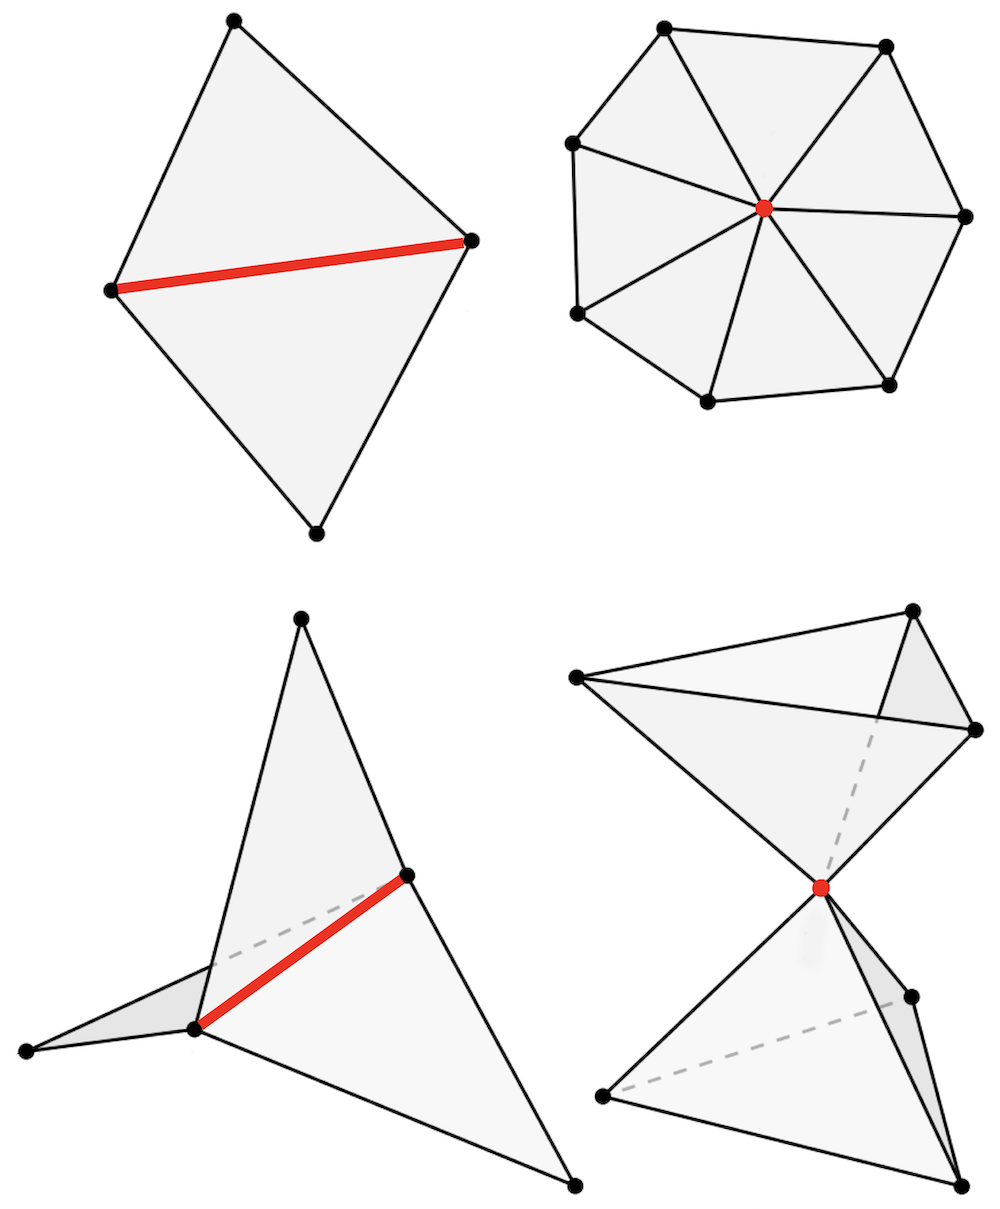
\includegraphics[width=0.9\linewidth]{figures/mesh.png}\\
%
Examples of manifold (top) and non-manifold (bottom) edges and nodes. 
For manifolds with boundary, one further defines {\em boundary edges} that belong to exactly one triangle. }
%
%We will denote meshes by $\mathcal{T} = (\mathcal{V},\mathcal{E}, \mathcal{F})$, where $\mathcal{F} =  \{ (i,j,k) : i,j,k \in \mathcal{V} \,\,\, \text{and} \,\,\, (i,j), (i,k), (k,j) \in  \mathcal{E}\}$ and use them as our domain $\Omega$.  


It is further assumed that that each edge is shared by exactly two triangles, and the boundary of all triangles incident on each node forms a single loop of edges. This condition guarantees that 1-hop neighbourhoods around each node are disk-like and the mesh thus constitutes a {\em discrete manifold} -- such meshes are referred to as {\em manifold meshes}. 
%In particular, 
%
%
%
Similarly to Riemannian manifolds, we can define a {\em metric} on the mesh. In the simplest instance, it can be  induced from the embedding of the mesh nodes $\mathbf{x}_1, \hdots, \mathbf{x}_n$ and expressed through the Euclidean length of the edges, $\ell_{uv} = \| \mathbf{x}_u - \mathbf{x}_v \|$. 
%
A metric defined in this way automatically satisfies properties such as the {\em triangle inequality}, i.e., expressions of the form 
$
\ell_{uv} \leq \ell_{uq} + \ell_{vq}
$
for any $(u,v,q) \in \mathcal{F}$ and any combination of edges. %
%
Any property that can be expressed solely in terms of $\ell$ is {\em intrinsic}, and any deformation of the mesh preserving $\ell$ is an {\em isometry}  -- these notions are already familiar to the reader from our discussion in Section~\ref{sec:manifolds}.   
%


%
%\paragraph{Mesh isometries and rigidity}
%Whether meshes have {\em non-trivial isometries} (i.e. embeddings that do not differ by only a rigid motion) is a deep question with fascinating history. %, and results here are starkly different from the continuous case. 
%%
%In 1766, Leonhard Euler conjectured that every polyhedron (a surface made of polygonal faces, on which a triangular mesh is a particular case) is {\em rigid}: that is, if one imagines a polyhedron as made of metal plates connected by hinges, it would not be possible to move them without bending. This assertion became known as the {\em Rigidity Conjecture} and gave birth to entire theory with the same name.  
%%
%\marginnote{
%\includegraphics[width=1\linewidth]{figures/connelly.png}\\
%%
%A convex polyhedron (icosahedron, left) is rigid by virtue of Cauchy's theorem. A non-convex polyhedron constructed by Klaus Steffen (right) is non-rigid and can be continuously deformed. 
%}
%%
%In 1813, Cauchy succeeded proving that every {\em convex} polyhedron is rigid in 3D \citep{cauchy1813recherche}. 
%%
%In 1897, a Belgian engineer and mathematician Raoul Bricard showed a construction of several flexible polyhedra \citep{bricard1897memoire}, which however, had self-intersections and thus could not be folded out of paper. 
%%
%In 1977, Robert Connelly showed  a non-rigid polyhedron without self-intersections (henceforth called the `Connelly Sphere') finally disproving Euler's conjecture by counter-example \citep{connelly1977counterexample}.  
%%
%A simpler (and in fact the simplest currently known) construction was shown a year later by the German geometry Klaus Steffen; his polyhedron can be easily folded of paper and bent {\em ad libitum}, as shown on the right. Admittedly, this is a very pleasant manual experience,  which the French {\em Institut des Hautes {\'E}tudes Scientifiques} in Bures-sur-Yvette wanted to share with the visitors, installing a metal model of a flexible polyhedron in its library. 
%\joan{This paragraph is very interesting, but it is unclear how it relates to the flow of the section. }

 





\paragraph{Laplacian matrices}
%
By analogy to our treatment of graphs, let us assume a (manifold) mesh with $n$ nodes, each associated with a $d$-dimensional feature vector, which we can arrange (assuming some arbitrary ordering) into an $n\times d$ matrix $\mathbf{X}$. 
%
The features can represent the geometric coordinates of the nodes as well as additional properties such as colors, normals, etc, or in specific applications such as chemistry where geometric graphs model molecules, properties such as the atomic number. 


Let us first look at the 
%construction of spectral filters following the 
spectral convolution~(\ref{eqn:conv_spectral}) on meshes, which we remind the readers, arises from the Laplacian operator. 
%
Considering the mesh as a discretisation of an underlying continuous surface, we can discretise the Laplacian  as 
%
\begin{equation}
(\boldsymbol{\Delta}\mathbf{X})_u = \sum_{v \in \mathcal{N}_u} w_{uv} (\mathbf{x}_u - \mathbf{x}_v),  
\label{eq:mesh_lap}
\end{equation}
%
or in matrix-vector notation, as an $n\times n$ symmetric matrix $\boldsymbol{\Delta} = \mathbf{D} - \mathbf{W}$, where $\mathbf{D} = \mathrm{diag}(d_1, \hdots, d_n)$ is called the {\em degree matrix} and $d_u = \sum_{v}w_{uv}$ the {\em degree} of node $u$.  
%
It is easy to see that equation~(\ref{eq:mesh_lap}) performs  local permutation-invariant aggregation of neighbour features $\phi(\mathbf{x}_u,\mathbf{X}_{\mathcal{N}_u}) =  d_u \mathbf{x}_u - \sum_{v \in \mathcal{N}_u} w_{uv} \mathbf{x}_v$, and $\mathbf{F}(\mathbf{X}) = \boldsymbol{\Delta}\mathbf{X}$ is in fact an instance of our general blueprint~(\ref{eq:graph_equivariant}) for constructing permutation-equivariant functions on graphs. 
%or, in matrix-vector notation as $\boldsymbol{\Delta} = %\mathbf{D}^{-1}\mathbf{W}$. 


Note that insofar there is nothing {\em specific to meshes} in our definition of Laplacian in~(\ref{eq:mesh_lap}); in fact, this construction is valid for arbitrary graphs as well, with edge weights identified with the adjacency matrix, $\mathbf{W} = \mathbf{A}$, i.e., $w_{uv} = 1$\marginnote{The degree in this case equals the number of neighbours. } if $(u,v) \in \mathcal{E}$ and zero otherwise.  
%
Laplacians constructed in this way are often called {\em combinatorial}, to reflect the fact that they merely capture the connectivity structure of the graph. \marginnote{If the graph is directed, the corresponding Laplacian is non-symmetric. }
%
For geometric graphs (which do not necessarily have the additional structure of meshes, but whose nodes do have spatial coordinates that induces a metric in the form of edge lengths), it is common to use weights inversely related to the metric, e.g. $w_{uv} \propto e^{-\ell_{uv}}$. 



On meshes, we can exploit the additional structure afforded by the faces, and define the edge weights in equation~(\ref{eq:mesh_lap}) using the {\em cotangent formula} \citep{pinkall1993computing,meyer2003discrete}\marginnote{
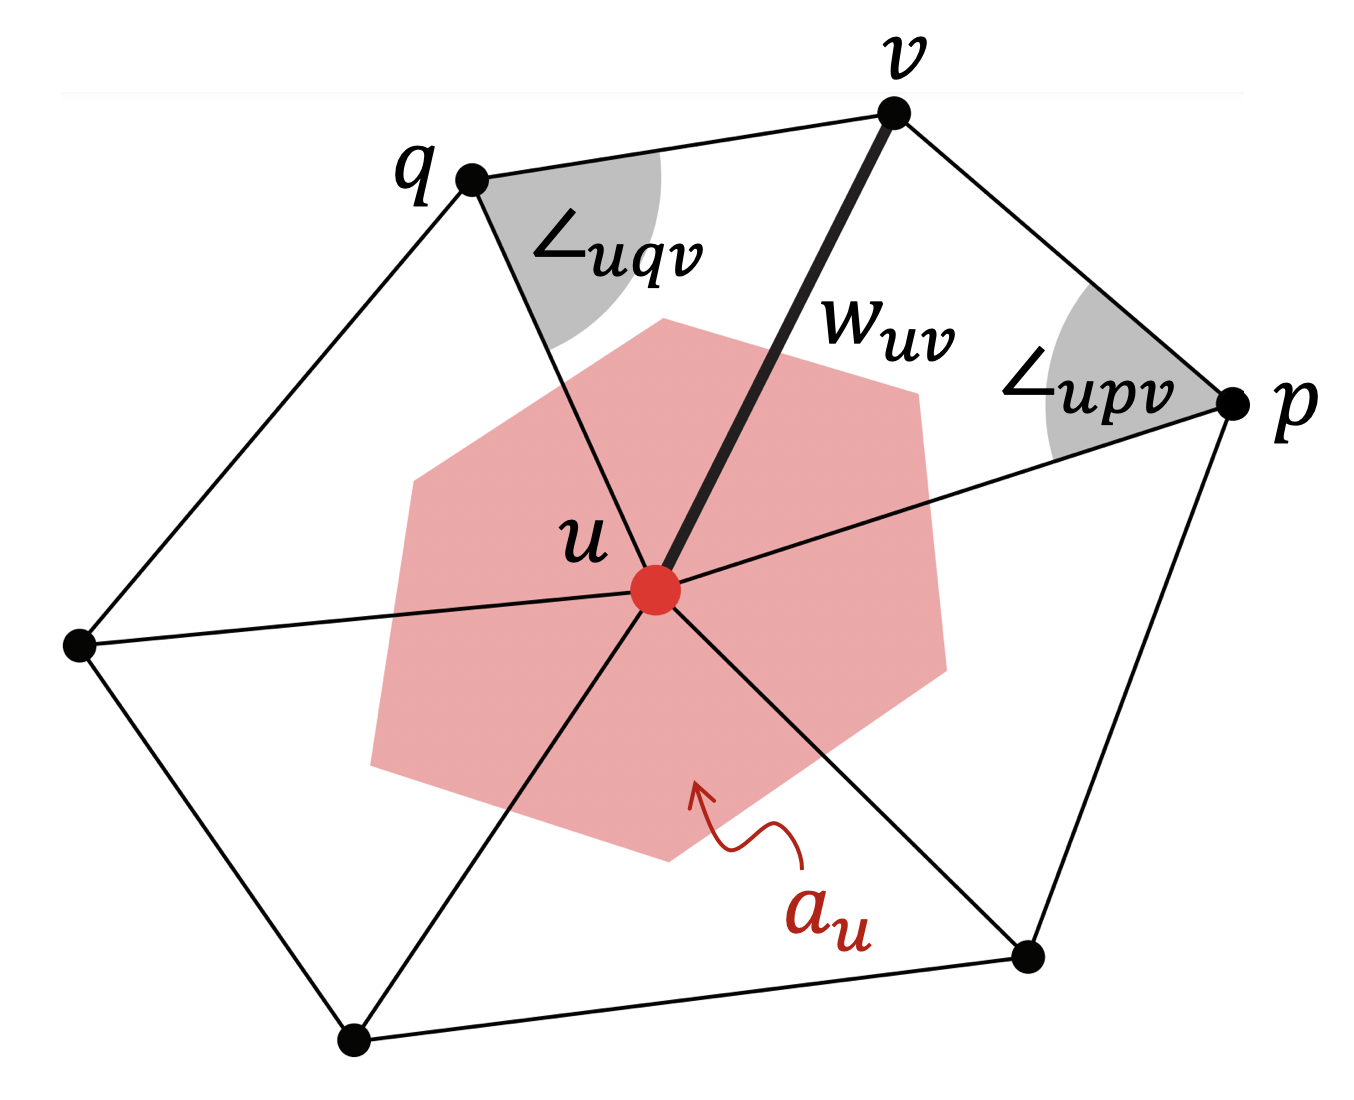
\includegraphics[width=\linewidth]{figures/cotan.png}
The earliest use of this formula dates back to the PhD thesis of \cite{macneal1949solution}, who developed it to solve PDEs on the Caltech Electric Analog Computer.}
\begin{equation}
w_{uv} = \frac{\cot \angle_{uqv} + \cot \angle_{upv}}{2 a_u}
\label{eq:cotan}
\end{equation}
where $\angle_{uqv}$ and $\angle_{upv}$ are the two angles in the triangles $(u,q,v)$ and $(u,p,v)$ opposite the shared edge $(u,v)$, and $a_u$ is the local area element, typically computed as the area of the polygon constructed upon the barycenters of the triangles $(u,p,q)$ sharing the node $u$ and given by
%
$a_u = \frac{1}{3}\sum_{v,q : (u,v,q) \in \mathcal{F}} a_{uvq}$.


The cotangent Laplacian can be shown to have multiple convenient properties (see e.g. \cite{wardetzky2007discrete}): it is a {\em positive-semidefinite} matrix, $\boldsymbol{\Delta} \succcurlyeq 0$ and thus has non-negative eigenvalues $\lambda_1 \leq \hdots \leq \lambda_n$ that can be regarded as an analogy of frequency, it is symmetric and thus has orthogonal eigenvectors, and it is {\em local} (i.e., the value of $(\boldsymbol{\Delta}\mathbf{X})_u$ depends only on 1-hop neighbours, $\mathcal{N}_u$).
%
Perhaps the most important property is the convergence of the cotangent mesh Laplacian matrix $\boldsymbol{\Delta}$ to the continuous operator $\Delta$ when the mesh is infinitely refined \citep{wardetzky2008convergence}.  Equation~(\ref{eq:cotan}) constitutes thus an appropriate {\em discretisation}\marginnote{Some technical conditions must be imposed on the refinement, to avoid e.g. triangles becoming pathological. One such example is a bizarre triangulation of the cylinder known in German as the {\em Schwarzscher Stiefel} (Schwarz's boot) or in English literature as the `Schwarz lantern', proposed in 1880 by Hermann Schwarz, a German mathematician known from the Cauchy-Schwarz inequality fame. } of the Laplacian operator defined on Riemannian manifolds in Section~\ref{sec:manifolds}. 


While one expects the Laplacian to be intrinsic, this is not very obvious from equation~(\ref{eq:cotan}), and it takes some effort to % this construction is intrinsic: one can in fact
express the cotangent weights entirely in terms of the discrete metric $\ell$ as 
$$
w_{uv} = \frac{-\ell^2_{uv} + \ell^2_{vq} + \ell^2_{uq} }{8 a_{uvq}} + 
\frac{-\ell^2_{uv} + \ell^2_{vp} + \ell^2_{up} }{8 a_{uvp}}
$$
%
where the area of the triangles $a_{ijk}$ is given as  
$$
a_{uvq} = \sqrt{s_{uvq} (s_{uvq} - \ell_{uv}) (s_{uvq} - \ell_{vq}) (s_{uvq} - \ell_{uq}) }
$$
using {\em Heron's semiperimeter formula} with 
%$s_{ijk} = \frac{1}{2}(\ell_{ij} + \ell_{ik} + \ell_{jk})$. 
$s_{uvq} = \frac{1}{2}(\ell_{uv} + \ell_{uq} + \ell_{vq})$. 
%
%
This endows the Laplacian (and any quantities associated with it, such as its eigenvectors and eigenvalues) with {\em isometry invariance}, a property for which it is so loved in geometry processing and computer graphics (see an excellent review by \cite{wang2019intrinsic}): any deformation of the mesh that does not affect the metric $\ell$ (does not `stretch' or `squeeze' the edges of the mesh) does not change the Laplacian.



Finally, as we already noticed,\marginnote{
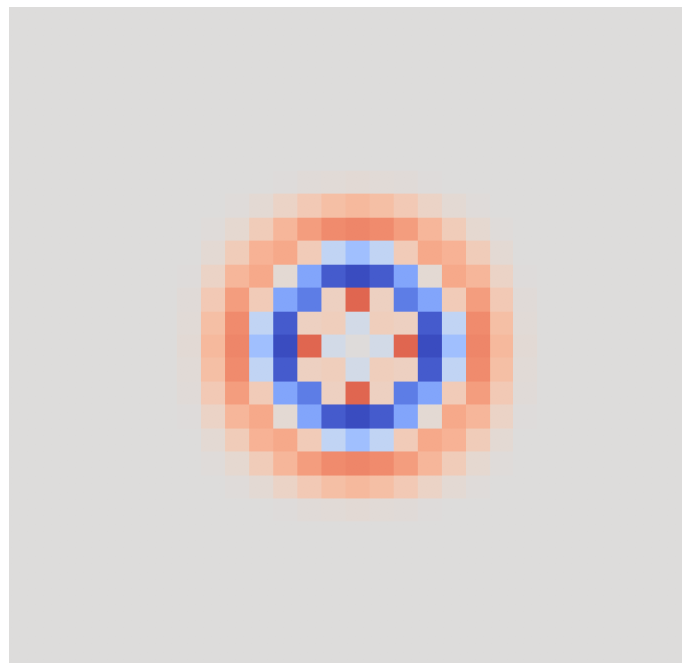
\includegraphics[width=0.9\linewidth]{figures/isotropic.png}
Laplacian-based filters are isotropic. In the plane, such filters have radial symmetry. 
} the definition of the Laplacian~(\ref{eq:cotan}) is invariant to the permutation of nodes in $\mathcal{N}_u$, as it involves aggregation in the form of summation. 
%
While on general graphs this is a necessary evil due to the lack of canonical ordering of neighbours, on meshes we can order the 1-hop neighbours according to some orientation (e.g., clock-wise), and the only ambiguity is the selection of the first node. Thus, instead of any possible permutation we need to account for {\em cyclic shifts} (rotations), which intuitively corresponds to the ambiguity arising from $\mathrm{SO}(2)$ gauge transformations discussed in Section~\ref{sec:gauges}. 
%
For a fixed gauge, it is possible to define an {\em anisotropic Laplacian} that is sensitive to local directions and amounts to changing the metric or the weights $w_{uv}$. 
%
Constructions of this kind were used to design shape descriptors by \cite{andreux2014anisotropic,boscaini2016anisotropic} and in early Geometric Deep Learning architectures on meshes by \cite{boscaini2016learning}. 



\paragraph{Spectral analysis on meshes}
%
The orthogonal eigenvectors $\boldsymbol{\Phi} = (\boldsymbol{\varphi}_1, \hdots, \boldsymbol{\varphi}_n)$ diagonalising the  Laplacian matrix ($\boldsymbol{\Delta} = \boldsymbol{\Phi} \boldsymbol{\Lambda} \boldsymbol{\Phi}^\top$, where $\boldsymbol{\Lambda} = \mathrm{diag}(\lambda_1, \hdots, \lambda_n)$ is the diagonal matrix of Laplacian eigenvalues), are used as the non-Euclidean analogy of the Fourier basis, allowing to perform spectral convolution on the mesh as the product of the respective Fourier transforms, 
$$
\mathbf{X} \star \boldsymbol{\theta} = 
\boldsymbol{\Phi} \, \mathrm{diag}(\boldsymbol{\Phi}^\top \boldsymbol{\theta}) (\boldsymbol{\Phi}^\top \mathbf{X}) 
=
\boldsymbol{\Phi}\, \mathrm{diag}(\hat{\boldsymbol{\theta}}) \hat{\mathbf{X}},
$$
%
where the filter $\hat{\boldsymbol{\theta}}$ is designed directly in the Fourier domain.  
%
Again, nothing in this formula is specific to meshes, and one can use the Laplacian matrix of a generic (undirected) graph.\marginnote{The fact that the graph is assumed to be undirected is important: in this case the Laplacian is symmetric and has orthogonal eigenvectors.}
%
%
It is tempting to exploit this spectral definition of convolution to generalise CNNs to graphs, which in fact was done by one of the authors of this text, \cite{bruna2013spectral}. 
%
However, it appears that the non-Euclidean Fourier transform 
is extremely sensitive to even minor perturbations of the underlying mesh or graph (see Figure~\ref{fig:mesh_horses} in Section~\ref{sec:manifolds}) and thus can only be used when one has to deal with different signals on a {\em fixed} domain, but not when one wishes to generalise across {\em different domains}. 
%
Unluckily, many computer graphics and vision problems fall into the latter category, where one trains a neural network on one set of 3D shapes (meshes) and test on a different set, making the Fourier transform-based approach inappropriate.  

%is given a training set of 3D shapes (meshes) and a different test, the generalisation across domains 



As noted in Section~\ref{sec:manifolds}, it is preferable to use spectral filters of the form~(\ref{eqn:conv_spec}) applying some transfer function $\hat{p}(\lambda)$ to the Laplacian matrix, 
$$
\hat{p}(\boldsymbol{\Delta})\mathbf{X} = \boldsymbol{\Phi} \hat{p}(\boldsymbol{\Lambda})\boldsymbol{\Phi}^\top\mathbf{X} 
= \boldsymbol{\Phi}\, \mathrm{diag}(\hat{p}(\lambda_1), \hdots, \hat{p}(\lambda_n)) \hat{\mathbf{X}}. 
$$
%
%which can be parametrised with a small number of parameters and computer efficiently. 
%
When $\hat{p}$ can be expressed in terms of matrix-vector products, the eigendecomposition of the $n\times n$ matrix $\boldsymbol{\Delta}$ \marginnote{In the general case, the complexity of eigendecomposition is $\mathcal{O}(n^3)$.} can be avoided altogether.  
%
For example, \cite{defferrard2016convolutional} used  {\em polynomials} of degree $r$ as filter functions, %in which case the filter is expressed as 
$$
\hat{p}(\boldsymbol{\Delta})\mathbf{X} = \sum_{k=0}^r \alpha_k \boldsymbol{\Delta}^k \mathbf{X}  = \alpha_0 \mathbf{X} + \alpha_1 \boldsymbol{\Delta} \mathbf{X}  + \hdots + \alpha_r \boldsymbol{\Delta}^r \mathbf{X}, 
$$
amounting to the multiplication of the $n\times d$ feature matrix $\mathbf{X}$ by the $n\times n$ Laplacian matrix $r$ times. Since the Laplacian is typically sparse (with $\mathcal{O}(|\mathcal{E}|)$ non-zero elements) \marginnote{Meshes are nearly-regular graphs, with each node having $\mathcal{O}(1)$ neighbours, resulting in $\mathcal{O}(n)$ non-zeros in $\boldsymbol{\Delta}$.  }
%
this operation has low complexity of $\mathcal{O}(|\mathcal{E}|dr)\sim \mathcal{O}(|\mathcal{E}|)$. 
%
Furthermore, since the Laplacian is local,  %(i.e., the value of $(\boldsymbol{\Delta}\mathbf{X})_i$ depends only on 1-hop neighbours, $\mathcal{N}_i$), 
a polynomial filter of degree $r$ is localised in $r$-hop neighbourhood. 


However, this exact property comes at a disadvantage when dealing with meshes, since the actual support of the filter (i.e., the radius it covers) depends on the {\em resolution} of the mesh. 
%
One has to bear in mind that meshes arise from the discretisation of some underlying continuous surface, and one may have two different meshes $\mathcal{T}$ and $\mathcal{T}'$ representing {\em the same object}. \marginnote{    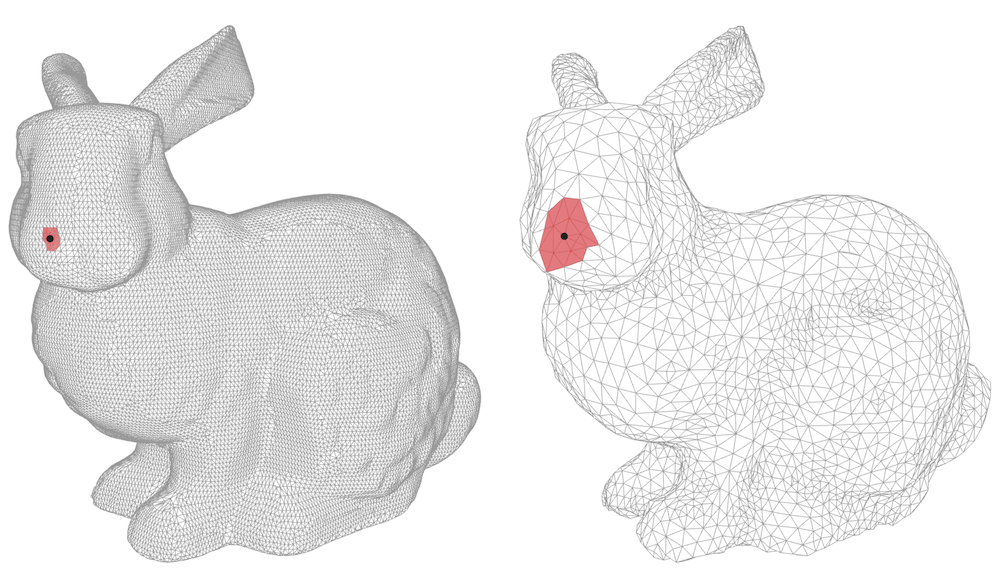
\includegraphics[width=\linewidth]{figures/mesh_res.png}\\
Two-hop neighbourhoods on meshes of different resolution. } 
%
In a finer mesh, one might have to use larger neighbourhoods (thus, larger degree $r$ of the filter) than in a coarser one. 
%

For this reason, in computer graphics applications it is more common to use {\em rational filters}, since they are  resolution-independent. There are many ways to define such filters (see, e.g. \cite{patane2020fourier}), the most common being as a polynomial of some  rational function, e.g., $\frac{\lambda-1}{\lambda+1}$. 
%
More generally, one can use a complex function, such as the {\em Cayley transform} $\frac{\lambda - \mi}{ \lambda + \mi}$ that maps the real line into the unit circle in the complex plane. \marginnote{Cayley transform is a particular case of a {\em M{\"o}bius transformation}. When applied to the Laplacian (a positive-semindefinite matrix), it maps its non-negative eigenvalues to the complex  half-circle. }
%
\cite{levie2018cayleynets} used spectral filters expressed as {\em Cayley polynomials}, real rational functions with complex coefficients $\alpha_l \in \mathbb{C}$,   
$$
\hat{p}(\lambda) = \mathrm{Re} \left(  \sum_{l=0}^r 
\alpha_l \left( \frac{\lambda - \mi}{ \lambda + \mi}
\right)^{l}
\right).
$$
%
When applied to matrices, the computation of the Cayley polynomial requires matrix inversion, 
$$
\hat{p}(\boldsymbol{\Delta}) = \mathrm{Re} \left(  \sum_{l=0}^r
\alpha_l (\boldsymbol{\Delta} - \mi\mathbf{I})^{l} (\boldsymbol{\Delta} + \mi\mathbf{I})^{-l}
\right),\marginnote{In signal processing, polynomial filters are termed {\em finite impulse response} (FIR), whereas rational filters are {\em infinite impulse response} (IIR).}
$$
which can be carried out approximately with linear complexity. 
%
Unlike polynomial filters, rational filters do not have a local support, but have exponential decay %and thus localised 
\citep{levie2018cayleynets}.  
%
A crucial difference compared to the direct computation of the Fourier transform is that polynomial and rational filters are stable under approximate isometric deformations of the underlying graph or mesh -- various results of this kind were shown e.g. by \cite{levie2018cayleynets,levie2019transferability,gama2020stability,kenlay2021interpretable}. 



%\paragraph{Anisotropic Laplacians}






\paragraph{Meshes as operators and Functional maps}


The paradigm of functional maps suggests thinking of meshes as {\em operators}. As we will show, this allows obtaining more interesting types of invariance exploiting the additional structure of meshes.  
%
For the purpose of our discussion, assume the mesh $\mathcal{T}$ is constructed upon embedded nodes with coordinates $\mathbf{X}$. 
%
If we construct an intrinsic operator like the Laplacian, it can be shown that it encodes completely the structure of the mesh, and one can recover the mesh (up to its isometric embedding, as shown by \cite{zeng2012discrete}). 
%
This is also true for some other operators (see e.g. \cite{boscaini2015shape,corman2017functional,chern2018shape}), so we will assume a general operator, or $n\times n$ matrix  $\mathbf{Q}(\mathcal{T}, \mathbf{X})$, as a representation of our mesh.  


In this view, the discussion of Section~\ref{sec:proto-graphs} of learning functions of the form   $f(\mathbf{X},\mathcal{T})$ %(as we had in our discussion on graphs in Section~\ref{sec:proto-graphs}) 
can be rephrased 
as learning functions of the form $f(\mathbf{Q})$. 
%
Similar to graphs and sets, the nodes of meshes also have no canonical ordering, i.e., functions on meshes must satisfy the permutation invariance or equivariance conditions, 
\begin{eqnarray*}
f(\mathbf{Q}) &=& f(\mathbf{P}\mathbf{Q}\mathbf{P}^\top) \\
%
\mathbf{P}\mathbf{F}(\mathbf{Q}) &=& \mathbf{F}(\mathbf{P}\mathbf{Q}\mathbf{P}^\top)
\end{eqnarray*}
% 
for any permutation matrix $\mathbf{P}$. 
%Conceptually, the permutation matrix can be considered as {\em correspondence} between two isomorphic meshes, i.e., meshes with the same number of nodes and identical connectivity. 
%
%
However, compared to general graphs we now have more structure: we can assume that our mesh arises from the discretisation of some underlying continuous surface $\Omega$. It is thus possible to have a different mesh  $\mathcal{T}'=(\mathcal{V}',\mathcal{E}',\mathcal{F}')$ with $n'$ nodes and coordinates $\mathbf{X}'$ representing the same object $\Omega$ as $\mathcal{T}$. 
%\marginnote{It is convenient to think of $\mathcal{T}'$ as a {\em remeshing} of $\mathcal{T}$.}  
%
%
Importantly, the meshes $\mathcal{T}$ and $\mathcal{T}'$ can have a different connectivity structure and even different number of nodes ($n'\neq n$). Therefore, we cannot think of these meshes as isomorphic graphs with mere reordering of nodes and consider the permutation matrix $\mathbf{P}$ as correspondence between them. 


Functional maps were introduced by \cite{ovsjanikov2012functional} as a generalisation of the notion of correspondence to such settings, replacing the correspondence between {\em points} on two domains (a map $\eta : \Omega \rightarrow \Omega'$) with correspondence between {\em functions} (a map $\mathbf{C}:\mathcal{X}(\Omega) \rightarrow \mathcal{X}(\Omega')$, see  Figure~\ref{fig:func_maps}). 
%
A {\em functional map} is a linear operator 
$\mathbf{C}$, represented as a matrix $n'\times n$,  establishing correspondence between signals $\mathbf{x}'$
%\in \mathcal{X}(\mathcal{T}')$  
%defined on the nodes of the mesh of $\mathcal{T}'$ 
and $\mathbf{x}$ % \in \mathcal{X}(\mathcal{T})$ as 
on the respective domains as 
%defined on the nodes of the mesh of $\mathcal{T}$ as 
$$
\mathbf{x}' = \mathbf{C}\mathbf{x}.\marginnote{
In most cases the functional map is implemented in the spectral domain, as a $k\times k$ map $\hat{\mathbf{C}}$ between the Fourier coefficients,
$
\mathbf{x}' = \boldsymbol{\Phi}'\hat{\mathbf{C}}\boldsymbol{\Phi}^\top\mathbf{x},
$
where $\boldsymbol{\Phi}$ and $\boldsymbol{\Phi}'$ are the respective $n\times k$ and $n'\times k$ matrices of the (truncated) Laplacian eigenbases, with $k\ll n,n'$. 
}
$$
%
%
%\michael{[TODO: Typically, $C$ is constructed in the Fourier domain - explain how. We want to have $C$ square to avoid problems with dimensions]}
\cite{rustamov2013map} showed that in order to guarantee {\em area-preserving} mapping, the functional map must be orthogonal, $\mathbf{C}^\top \mathbf{C} = \mathbf{I}$, i.e., be an element of the orthogonal group $\mathbf{C} \in \mathrm{O}(n)$. In this case, we can invert the map using $\mathbf{C}^{-1} = \mathbf{C}^\top$. 


\begin{figure}[h!]
    \centering
    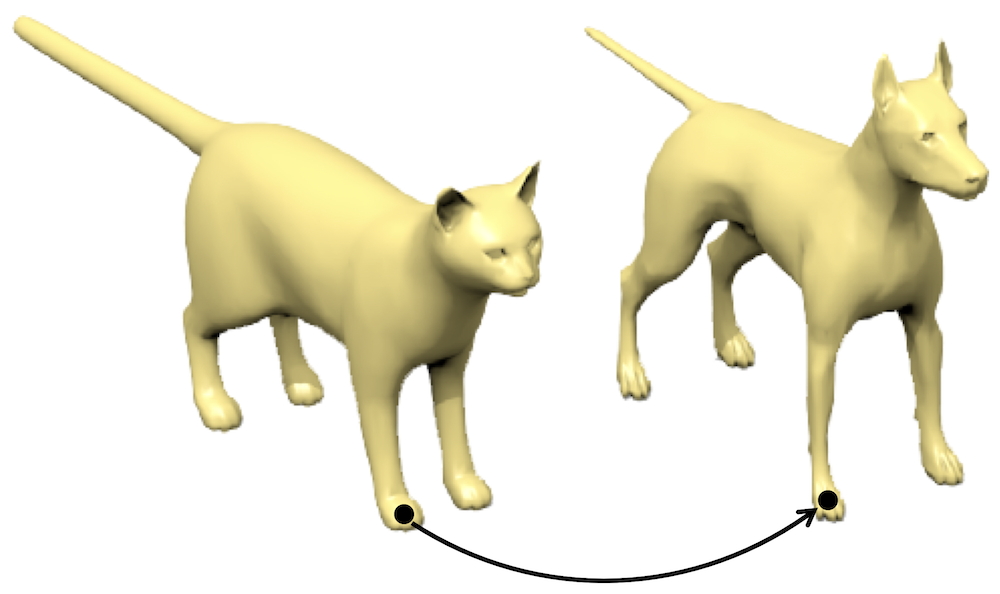
\includegraphics[width=0.45\linewidth]{figures/map_point.png}\hspace{5mm}    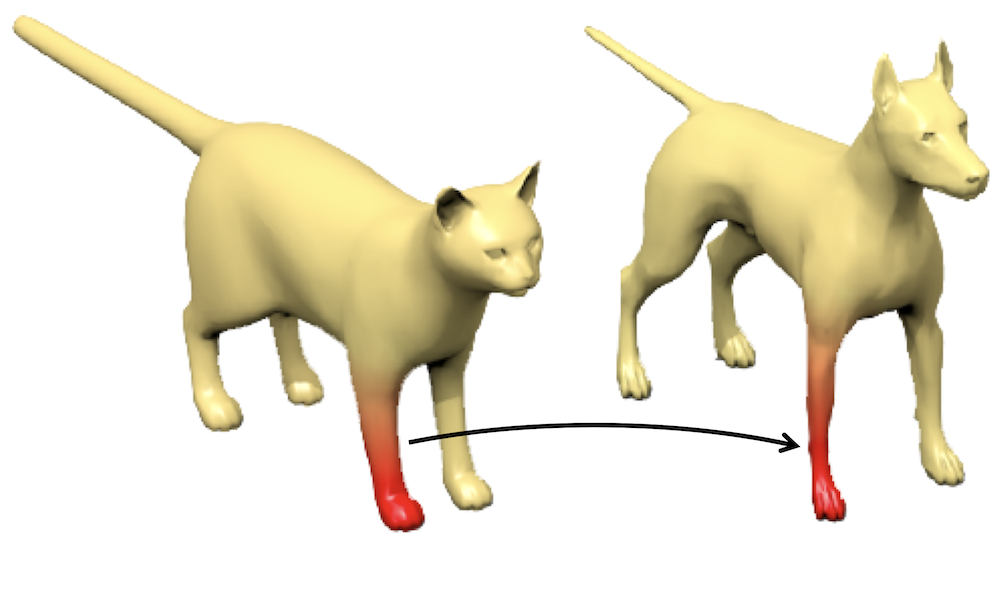
\includegraphics[width=0.45\linewidth]{figures/map_func.png}
    \caption{Pointwise map (left) vs functional map (right).   
    }
    \label{fig:func_maps}
\end{figure}%


The functional map also establishes a relation between the operator representation of meshes, 
$$
\mathbf{Q}' = \mathbf{C} \mathbf{Q} \mathbf{C}^\top, \quad \quad \mathbf{Q} = \mathbf{C}^\top \mathbf{Q}' \mathbf{C}, 
$$
%
which we can interpret as follows: given an operator representation $\mathbf{Q}$ of $\mathcal{T}$ and a functional map $\mathbf{C}$, we can construct its representation $\mathbf{Q}'$ of $\mathcal{T}'$ by first mapping the signal from $\mathcal{T}'$ to $\mathcal{T}$ (using $\mathbf{C}^\top$), applying the operator $\mathbf{Q}$, and then mapping back to $\mathcal{T}'$ (using $\mathbf{C}$)\marginnote{Note that we read these operations \emph{right-to-left}. }
%, i.e. we assume left-multiplication with a signal on $\mathcal{T}'$.}. 
%
This leads us to a more general class of {\em remeshing  invariant} (or equivariant) functions on meshes, satisfying 
%
\begin{eqnarray*}
f(\mathbf{Q}) &=& f(\mathbf{C}\mathbf{Q}\mathbf{C}^\top) = f(\mathbf{Q}')\\
%
\mathbf{C}\mathbf{F}(\mathbf{Q}) &=& \mathbf{F}(\mathbf{C}\mathbf{Q}\mathbf{C}^\top) = \mathbf{F}(\mathbf{Q}')
\end{eqnarray*}
% 
for any $\mathbf{C} \in \mathrm{O}(n)$. 
%
It is easy to see that the previous setting of permutation invariance and equivariance is a particular case,  \marginnote{This follows from the orthogonality of permutation matrices, $\mathbf{P}^\top \mathbf{P} = \mathbf{I}$.}
which can be thought of as a trivial remeshing in which only the order of nodes is changed.


\cite{wang2019learning} showed that given an eigendecomposition of the operator $\mathbf{Q} = \mathbf{V}\boldsymbol{\Lambda}\mathbf{V}^\top$, any remeshing invariant (or equivariant) function can be expressed as 
%
%
$f(\mathbf{Q}) = f(\boldsymbol{\Lambda})$ and 
%
$\mathbf{F}(\mathbf{Q}) = \mathbf{V} \mathbf{F}(\boldsymbol{\Lambda})$, 
%
or in other words, remeshing-invariant functions {\em involve only the spectrum of} $\mathbf{Q}$. 
%
%
Indeed, functions of Laplacian eigenvalues have been proven in practice to be robust to surface discretisation and perturbation, explaining the popularity of spectral constructions based on Laplacians in computer graphics, as well as in deep learning on graph \citep{defferrard2016convolutional,levie2018cayleynets}. 
%
%In graph deep learning literature, architectures such as ChebNet \citep{defferrard2016convolutional} and CayleyNet \citep{levie2018cayleynets} explicitly learn functions of Laplacian eigenvalues. 
%
%
Since this result refers to a generic operator $\mathbf{Q}$, multiple choices are available besides the ubiquitous Laplacian -- notable examples include the Dirac \citep{liu2017dirac,kostrikov2018surface} or Steklov \citep{wang2018steklov} operators, as well as learnable parametric operators \citep{wang2019learning}. 


%\michael{The degree of freedom we have is the operator itself - which leads to learnable operators.}

%\joan{We might want to mention extrinsic models that build anisotropy based on the Dirac Operator rather than the Laplace operator; Crane et al, and our Surface Network paper}
%\joan{This section clearly needs to branch out into its own chapter. }




\section{Geometric Deep Learning Models}

Having thoroughly studied various instantiations of our Geometric Deep Learning blueprint (for different choices of domain, symmetry group, and notions of locality), we are ready to discuss how enforcing these prescriptions can yield some of the most popular deep learning architectures.

Our exposition, once again, will not be in strict order of generality. We initially cover three architectures for which the implementation follows nearly-directly from our preceding discussion: convolutional neural networks (CNNs), group-equivariant CNNs, and graph neural networks (GNNs).

We will then take a closer look into variants of GNNs for cases where a graph structure is not known upfront (i.e. unordered sets), and through our discussion we will describe the popular Deep Sets and Transformer architectures as instances of GNNs.

Following our discussion on geometric graphs and meshes, we first describe equivariant message passing networks, which introduce explicit geometric symmetries into GNN computations. Then, we show ways in which our theory of geodesics and gauge symmetries can be materialised within deep learning, recovering a family of intrinsic mesh CNNs (including Geodesic CNNs, MoNet and gauge-equivariant mesh CNNs).

Lastly, we look back on the grid domain from a \emph{temporal} angle. This discussion will lead us to recurrent neural networks (RNNs). We will demonstrate a manner in which RNNs are translation equivariant over temporal grids, but also study their stability to time warping transformations. This property is highly desirable for properly handling long-range dependencies, and enforcing class invariance to such transformations yields exactly the class of gated RNNs (including popular RNN models such as the LSTM or GRU). %Given that we aim to study time warping invariance in greater detail (and not just describe a model class), this subsection will be longer than the others. 

While we hope the above canvasses most of the key deep learning architectures in use at the time of writing, we are well aware that novel neural network instances are proposed daily. Accordingly, rather than aiming to cover every possible architecture, we hope that the following sections are illustrative enough, to the point that the reader is able to easily categorise any future Geometric Deep Learning developments using the lens of invariances and symmetries.

\subsection{Convolutional Neural Networks}
\label{sec:cnnsec}

Convolutional Neural Networks are perhaps the earliest and most well known  example of deep learning architectures following the blueprint of Geometric Deep Learning outlined in Section~\ref{sec:gdl_blueprint}. 
%
%
% ====
%
In Section \ref{sec:grids_euclidean} we have fully characterised the class of linear and local translation equivariant operators, given by 
convolutions ${\bf C(\thetab)}{\bf x} = {\bf x} \star \thetab$ with a localised filter $\thetab$\marginnote{Recall, ${\bf C}(\boldsymbol{\theta})$ is a \emph{circulant} matrix with parameters $\boldsymbol{\theta}$.}. 
Let us first focus on scalar-valued (`single-channel' or `grayscale') discretised images,  
%${\bf x}$ (having a single channel), 
where 
the domain is the grid $\Omega = [H] \times [W]$ with $\mathbf{u} = (u_1, u_2)$ and ${\bf x} \in \gX(\Omega, \R)$.

Any convolution with a compactly supported filter of size $H^f \times W^f$
can be written as a linear combination of 
generators $\thetab_{1,1}, \dots, \thetab_{{H^f,W^f}}$, given for example by the unit peaks $\boldsymbol{\theta}_{vw}(u_1, u_2) = \delta(u_1 - v, u_2 - w)$. Any local linear equivariant map is thus expressible as\marginnote{Note that we usually imagine $\vec{x}$ and $\boldsymbol{\theta}_{vw}$ as 2D matrices, but in this equation, both $\vec{x}$ and $\boldsymbol{\theta}_{vw}$ have their two coordinate dimensions \emph{flattened} into one---making $\vec{x}$ a vector, and $\vec{C}(\boldsymbol{\theta}_{vw})$ a matrix.} %directional derivatives $\thetab_{ij}(u_1,u_2) = \delta(u_1, u_2) - \delta(u_1-i,u_2-j), (i,j) \neq (0,0) $ plus the local average $\thetab_{0}(u_1,u_2) = \Delta^{-2}$. % \taco{I guess delta here is a function that equals 1 at (0,0) and 0 elsewhere? Could also mean 1 when u1 = u2, or it could be the Dirac delta which is infinite at zero... Maybe clarify. Also if my first guess is correct, is this really a basis? Can we express the filter which is 1 in the center and 0 elsewhere, i.e. delta(u1, u2)? Finally, just using a basis of delta peaks on each pixel might be more intuitive than directional derivatives?}
%\joan{Yes, here we used directional derivatives as analogy with graphs, in which derivative filters (Adjacency being lowpass filter and Laplacian being high-pass) are intrinsically defined. Correct I missed the average in the family of generators }
\begin{equation}
    \mathbf{F}(\mathbf{x}) = \sum_{v=1}^{H^f}\sum_{w=1}^{W^f} \alpha_{vw} \mathbf{C}(\thetab_{vw})\mathbf{x}~, 
\end{equation}
which, in coordinates, corresponds to the familiar 2D convolution (see Figure \ref{fig:2dconv} for an overview):
\begin{figure}
     \centering
     \includegraphics[width=0.7\linewidth]{figures/2d_conv.pdf}
     \caption{The process of convolving an image $\vec{x}$ with a filter $\vec{C}(\boldsymbol{\theta})$. The filter parameters $\boldsymbol{\theta}$ can be expressed as a linear combination of generators $\boldsymbol{\theta}_{vw}$.}
     \label{fig:2dconv}
\end{figure}
\begin{equation}\mathbf{F}(\mathbf{x})_{uv}= \sum_{a=1}^{H^f}\sum_{b=1}^{W^f} {\alpha}_{ab} x_{u+a, v+b}~.
\end{equation}
Other choices of the basis $\boldsymbol{\theta}_{vw}$ are also possible and will yield equivalent operations (for potentially different choices of $\alpha_{vw}$). A popular example are \emph{directional derivatives}: $\thetab_{vw}(u_1,u_2) = \delta(u_1, u_2) - \delta(u_1-v,u_2-w), (v,w) \neq (0,0) $ taken together with the local average $\thetab_{0}(u_1,u_2) = \frac{1}{H_fW_f}$. In fact, directional derivatives can be considered a grid-specific analogue of diffusion processes on graphs, which we recover if we assume each pixel to be a node connected to its immediate neighbouring pixels in the grid.

When the scalar input channel is replaced by multiple channels (e.g., RGB colours, or more generally an arbitrary number of \emph{feature maps}), the convolutional filter becomes a {\em convolutional tensor} expressing arbitrary linear combinations of input features into output feature maps. In coordinates, this can be expressed as 
%
\begin{equation}
\label{eq:basiccnnlayer}
\mathbf{F}(\mathbf{x})_{uvj}= \sum_{a=1}^{H^f}\sum_{b=1}^{W^f}\sum_{c=1}^M {\alpha}_{jabc} x_{u+a, v+b, c}~,~ j\in[N]~,
\end{equation}
%
where $M$ and $N$ are respectively the number of input and output channels. 
This basic operation encompasses a broad class of neural network architectures, which, as we will show in the next section, have had a profound impact across many areas of computer vision, signal processing, and beyond. Here, rather than dissecting the myriad of possible architectural variants of CNNs, we prefer to focus on some of the essential innovations that enabled their widespread use.  



\paragraph{Efficient multiscale computation} 
As discussed in the GDL template for general symmetries, extracting translation invariant features out of the convolutional operator $\mathbf{F}$ requires a non-linear step.\marginnote{\includegraphics[width=\linewidth]{figures/relu.pdf}\\ ReLU, often considered a `modern' architectural choice, was already used in the Neocognitron \citep{fukushima1982neocognitron}. Rectification is equivalent to the principle of demodulation, which is fundamental in electrical engineering as the basis for many transmission protocols, such as FM radio; and also has a prominent role in models for neuronal activity.} %so that the energy captured along each sub-band $\thetab_{ij}$ is mapped towards the low-frequencies
Convolutional features are processed through a non-linear %rectification stage, 
\emph{activation function} $\sigma$, acting element-wise on the input---i.e., $\sigma: \gX(\Omega) \to \gX(\Omega)$, as $\sigma(\mathbf{x})(u) = \sigma(\mathbf{x}(u))$. Perhaps the most popular example at the time of writing is the Rectified Linear Unit (ReLU): $\sigma(x) = \max(x, 0)$. %, or other choices of activation function. 
This non-linearity effectively \emph{rectifies} the signals, pushing their energy towards lower frequencies, and enabling the computation of high-order interactions across scales by iterating the construction.

Already in the early works of \cite{fukushima1982neocognitron} and \cite{lecun1998gradient}, CNNs and similar architectures 
%Since the early days from Fukushima and LeCun, CNN architectures 
had a multiscale structure, where after each convolutional layer (\ref{eq:basiccnnlayer}) one performs a grid coarsening 
$\mathbf{P} : \gX(\Omega) \to \gX(\Omega')$, where the grid $\Omega'$ has coarser resolution than $\Omega$. 
This enables 
multiscale filters with effectively increasing receptive field, yet retaining a constant number of parameters per scale. 
%
Several signal coarsening %or  
strategies $\mathbf{P}$ (referred to as \emph{pooling}) may be used, the most common are %possible: either %by %explicitly 
applying a low-pass anti-aliasing filter (e.g. local average) followed by grid downsampling, or non-linear max-pooling. 
%
%
%Inspired by neuroscience, 

In summary, a `vanilla' CNN layer can be expressed as the composition of the basic objects already introduced in our Geometric Deep Learning blueprint:
\begin{equation}
    \mathbf{h} = \mathbf{P}(\sigma(\mathbf{F}( \mathbf{x})))~,
\end{equation}
i.e. an equivariant linear layer $\mathbf{F}$, a coarsening operation $\mathbf{P}$, and a non-linearity $\sigma$. It is also possible to perform translation invariant \emph{global} pooling operations within CNNs. Intuitively, this involves each pixel---which, after several convolutions, summarises a \emph{patch} centered around it---\emph{proposing} the final representation of the image\marginnote{CNNs which only consist of the operations mentioned in this paragraph are often dubbed ``all-convolutional''. In contrast, many CNNs \emph{flatten} the image across the spatial axes and pass them to an MLP classifier, once sufficient equivariant and coarsening layers have been applied. This loses translation invariance.}, with the ultimate choice being guided by a form of aggregation of these proposals. A popular choice here is the average function, as its outputs will retain similar magnitudes irrespective of the image size \citep{springenberg2014striving}.

Prominent examples following this CNN blueprint (some of which we will discuss next) are displayed in Figure \ref{fig:cnn_drawn_plot}.

\begin{figure}
    \centering
    \includegraphics[width=0.85\textwidth]{figures/lenet.pdf}
    \includegraphics[width=0.85\textwidth]{figures/alexnet.pdf}
    \includegraphics[width=0.85\textwidth]{figures/resnet.pdf}
    \includegraphics[width=0.85\textwidth]{figures/Unet.pdf}
    \caption{Prominent examples of CNN architectures. \textbf{Top-to-bottom}: LeNet \citep{lecun1998gradient}, AlexNet \citep{krizhevsky2012imagenet}, ResNet \citep{he2016deep} and U-Net \citep{ronneberger2015u}. Drawn using the PlotNeuralNet package \citep{haris2018}.}
    \label{fig:cnn_drawn_plot}
\end{figure}
%role of depth
\paragraph{Deep and Residual Networks}
A CNN architecture, in its simplest form, is therefore specified by hyperparameters $(H^f_k, W^f_k, N_k, p_k )_{k \leq K}$, with $M_{k+1} = N_k$ and $p_k=0,1$ indicating whether grid coarsening is performed or not. While all these hyperparameters are important in practice, a particularly important  question is to understand the role of depth $K$ in CNN architectures, and what are the fundamental tradeoffs involved in choosing such a key hyperparameter, especially in relation to the filter sizes ($H_k^f, W_k^f$). 

While a rigorous answer to this question is still elusive, mounting empirical evidence collected throughout the recent years suggests a favourable tradeoff towards deeper (large $K$) yet thinner (small $(H^f_k, W^f_k)$) models \marginnote{
Historically, ResNet models are predated by \emph{highway networks} \citep{srivastava2015highway}, which allow for more general \emph{gating} mechanisms to control the residual information flow.}. In this context, a crucial insight by \cite{he2016deep} was to reparametrise each convolutional layer to model a \emph{perturbation} of the previous features, rather than a generic non-linear transformation:
\begin{equation}
    \mathbf{h} = \mathbf{P}\left(\mathbf{x} + \sigma(\mathbf{F}(\mathbf{x})) \right)~.
\end{equation}
The resulting \emph{residual} networks provide several key advantages over the previous formulation. In essence, the residual parametrisation is consistent with the view that the deep network is a discretisation of an underlying continuous dynamical system, modelled as an ordinary differential equation (ODE)\marginnote{In this case, the ResNet is performing a Forward Euler discretisation of an ODE: $\dot{\mathbf{x}} = \sigma( \mathbf{F}(\mathbf{x}))$}. Crucially, learning a dynamical system by modeling its velocity turns out to be much easier than learning its position directly. In our learning setup, this translates into an optimisation landscape with more favorable geometry, leading to the ability to train much deeper architectures than was possible before. As will be discussed in future work, learning using deep neural networks defines a non-convex optimisation problem, which can be efficiently solved using gradient-descent methods under certain simplifying regimes. The key advantage of the ResNet parametrisation has been rigorously analysed in simple scenarios \citep{hardt2016identity}, and remains an active area of theoretical investigation. 
Finally, Neural ODEs \citep{chen2018neural} are a recent popular architecture that pushes the analogy with ODEs even further, by learning the parameters of the ODE $\dot{\mathbf{x}} = \sigma( \mathbf{F}(\mathbf{x}))$ directly and relying on standard numerical integration. 

%\michael{This is also the case for GNNs, which are a discretization of a nonlinear diffusion PDE} \petar{skipping for now, as discussed with Michael}

%Normalization 
\paragraph{Normalisation} 
Another important algorithmic innovation that boosted the empirical performance of CNNs significantly is the notion of \emph{normalisation}. In early models of neural activity, it was hypothesised that neurons perform some form of local `gain control', where the layer coefficients $\mathbf{x}_{k}$ are replaced by $\mathbf{\tilde{x}}_{k} = \sigma_k^{-1} \odot (\mathbf{x}_{k} - \mu_k)$. Here, $\mu_k$ and $\sigma_k$ encode the first and second-order moment information of $\mathbf{x}_k$, respectively. Further, they can be either computed globally or locally.

In the context of Deep Learning, this principle was widely adopted through the \emph{batch normalisation} layer \citep{ioffe2015batch}\marginnote{We note that normalising activations of neural networks has seen attention even before the advent of batch normalisation. See, e.g., \cite{lyu2008nonlinear}.}, followed by several variants \citep{ba2016layer,salimans2016weight,ulyanov2016instance,cooijmans2016recurrent,wu2018group}. 
Despite some attempts to rigorously explain the benefits of normalisation in terms of better conditioned optimisation landscapes \citep{santurkar2018does}, a general theory that can provide guiding principles is still missing at the time of writing.  

\paragraph{Data augmentation}
While CNNs encode the geometric priors associated with translation invariance and scale separation, they do not explicitly account for other known transformations that preserve semantic information, e.g lightning or color changes, or small rotations and dilations. A pragmatic approach to incorporate these priors with minimal architectural changes is to perform \emph{data augmentation}, where one manually performs said transformations to the input images and adds them into the training set.

Data augmentation has been empirically successful and is widely used---not only to train state-of-the-art vision architectures, but also to prop up several developments in self-supervised and causal representation learning \citep{chen2020simple,grill2020bootstrap,mitrovic2020representation}. However, it is provably sub-optimal in terms of sample complexity \citep{mei2021learning}; a more efficient strategy considers instead architectures with richer invariance groups---as we discuss next.

%TODO: discuss Preserving Orientation: contrast this with the GNN setting. 

% ====

% To define a convolutional operator, we will consider the case of 2D inputs (i.e. single-channel images), $\vec{X}\in\mathbb{R}^{h\times w}$. Let $\vec{K}\in\mathbb{R}^{n\times m}$ be a small \emph{kernel matrix} (typically, $n = m = 3$ in modern neural network architectures). The kernel is overlaid in all possible ways
% over the input (see Figure \ref{fig:2dconv}), recording sums of elementwise products to create a
% new image, $\vec{X}'$:\marginnote{It should be noted that this approach is actually cross‐correlation rather than the convolution; but, for purposes of machine learning, the two are equivalent.}
% \begin{equation}
%     x'_{ab} = \sum_{i=1}^n\sum_{j=1}^m k_{ij}x_{a+i-1,b+j-1}
% \end{equation}
% The image is typically padded with sufficiently many zeroes on the edges, to ensure that the size of the output matches the size of the input.

% Moving from here to a convolutional \emph{layer} requires a few extensions. If the input has multiple channels, the kernel matrix is \emph{extended} in the channel dimension to match the input. This \emph{kernel tensor} specifies a single output channel. Each output channel requires a separate kernel tensor. Lastly, a channel‐specific bias and nonlinearity may be applied to obtain the final output image (sometimes known as a \emph{feature map}). 

% In summary, to process an input image $\vec{X} \in \mathbb{R}^{h\times w\times d}$ using a convolutional layer computing $d'$ channels, we require a kernel tensor $\vec{K}\in\mathbb{R}^{n\times m\times d\times d'}$ and a bias vector $\vec{b}\in\mathbb{R}^{d'}$, and proceed as follows:\marginnote{\includegraphics[width=\linewidth]{figures/fullconv.png}}
% \begin{equation}
%     x'_{abc} = \sigma\left(b_c + \sum_{i=1}^n\sum_{j=1}^m\sum_{k=1}^d k_{ijkc}x_{a+i-1,b+j-1,k}\right)
% \end{equation}

% This layer clearly exploits the structure present in an image, with neighbouring pixels
% influencing each other far more strongly than ones on opposite corners. The operator is
% also \emph{translation equivariant}, as required for grids: as the same kernels are applied identically across each image patch, we are encoding a structural bias that a feature of interest is important, no matter where it occurs in the image.

% Often, we are interested in computing outputs on the level of \emph{entire} images. Hence it is useful to compress an image to a \emph{flat} representation, but doing so on the input image sizes often results in an overly large vector (of size $O(hwd)$. Accordingly, once a sufficient number of convolutions has been applied to the input, it is very common to \emph{downsample} the image. 

% As convolutions \emph{``light up''}\marginnote{\includegraphics[width=\linewidth]{figures/maxpool.png}} (return high values) when a certain
% pattern of interest is detected in the input, when summarising the image it makes sense
% to preserve \emph{maximally activated} components of it. This motivates the \emph{max‐pooling} layer, which takes $n\times m$ (usually disjoint, with $n = m = 2$) image patches across each channel and summarises them by taking only the maximal pixel value.

% \michael{This is certainly not the most important reason for using nonlinear pooling - I think we want to refer to Bruna, Mallat 2012 here}

% \begin{figure}
%     \centering
%     \includegraphics[width=\linewidth]{figures/fig_conv.png}
%     \caption{An overview of a typical CNN architecture for image classification. Convolutional and pooling layers are interleaved, with the depth (number of features computed per pixel) increased at the expense of height and width. Once the images are small enough, they are flattened into 1D, and an MLP is used to classify them.}
%     \label{fig:figconv}
% \end{figure}

% Note that a $2\times 2$ max‐pooling layer (which is most common) will preserve only a quarter of the pixels, while leaving the channel axis unchanged. This provides more space
% for gradually increasing the channel size, and therefore computing a richer quantity of
% higher‐level features. A typical convolutional neural network architecture thus consists
% of a series of interleaved convolutional and pooling layers, until the input is reduced sufficiently to be processed by an MLP---as in Figure \ref{fig:figconv}.

% It is also possible, though less common, to perform \emph{global} pooling operations within CNNs. Intuitively, this involves each pixel---which, after several convolutions, summarises a \emph{patch} centered around it---\emph{proposing} the final representation of the image, with the ultimate choice being guided by a form of aggregation of these proposals. A popular choice here is the average function, as its outputs will retain similar magnitudes irrespective of the image size \citep{springenberg2014striving}.

% It is generally perceived that, for image recognition tasks, deep convolutional networks
% strongly draw their outperformance from both their depth \textbf{and} their parameter tying. However, training very deep convolutional networks used to be notoriously difficult. As shown by \citet{he2016deep}, overly deep convolutional networks \emph{do not overfit}, as their training performance degrades along with their testing performance. This is somewhat counterintuitive, as increased depth not only comes with larger parameter spaces to optimise, but moreover, if the additional layers are useless to learning good representations,
% the layer could simply choose to \emph{ignore} them (by learning the \textbf{identity} function).

% Through this counterintuitive property, the authors proposed an obvious fix: the \emph{residual (skip) connection} \citep{he2016deep}, which ``shortcuts'' a particular block of operations in a neural
% network. If a neural network block computes a function $f(\vec{x})$, a skip connection allows $\vec{X}$ to directly reach the output of this block through aggregation; i.e. the neural network simply computes $f(\vec{x}) + \vec{x}$. More generally, if the block changes the input dimensionality, a simple linear projection may be introduced to correct for this:
% \begin{equation}
%     \widetilde{f}(\vec{x}) = f(\vec{x}) + \vec{W}_\mathrm{skip}\vec{x} 
% \end{equation}
% Note that, effectively, this operation allows signals to directly reach deeper stages of the
% input processing, and therefore allows the network to choose its own depth. This turned
% out to be a very powerful and versatile concept, that enabled a 152‐layer network to win
% the ImageNet competition in 2015. Currently, it is ubiquitous in deep learning. It is worth noting that such (``ResNet'') models are predated by \emph{highway networks} \citep{srivastava2015highway}, which allow for more general \emph{gating} mechanisms to control the residual information flow.

% \michael{Scale separation and pooling - show here how pooling makes approximate translation invariance?}





\subsection{Group-equivariant CNNs}

As discussed in Section \ref{sec:groups}, we can generalise the convolution operation from signals on a Euclidean space to signals on any \emph{homogeneous space} $\Omega$ acted upon by a group $\fG$\marginnote{Recall that a homogeneous space is a set $\Omega$ equipped with a transitive group action, meaning that for any $u,v \in \Omega$ there exists $\fg \in \fG$ such that $\fg. u = v$.}.
By analogy to the Euclidean convolution where a {\em translated} filter is matched with the signal, the idea of group convolution is to move the filter around the domain using the group action, e.g. by rotating and translating. 
By virtue of the \emph{transitivity} of the group action, we can move the filter to any position on $\Omega$.
In this section, we will discuss several concrete examples of the general idea of group convolution, including implementation aspects and architectural choices. 

%, including discrete roto-translation equivariant planar and 3D CNNs, convolutions on the group of symmetries of a DNA sequence, and spherical CNNs.

\paragraph{Discrete group convolution}

We begin by considering the case where the domain $\Omega$ as well as the group $\fG$ are discrete.
%
As our first example, we consider medical volumetric images represented as signals of on 3D grids %(e.g. medical scans) 
with discrete translation and rotation symmetries. %, 
%and DNA sequences with translation symmetry as well as so-called \emph{reverse-complement} symmetry (explained below).
%
%For the first example, we take as 
The domain is the 3D cubical grid $\Omega = \Z^3$ and the images (e.g. 
MRI or CT 3D scans) are modelled as functions $x : \Z^3 \rightarrow \R$, i.e. $x \in \mathcal{X}(\Omega)$.
Although in practice such images have support on a finite cuboid $[W] \times [H] \times [D] \subset \Z^3$, we instead prefer to view them as functions on $\Z^3$ with appropriate zero padding. 
%that happen to be zero outside a finite region. 
%
As our symmetry, we consider the group $\fG = \Z^3 \rtimes O_h$ of distance- and orientation-preserving transformations on $\Z^3$.
This group consists of translations ($\Z^3$) and the discrete rotations $O_h$ generated by $90$ degree rotations about the three axes (see Figure \ref{fig:cayley-diagram-Oh}).

\begin{figure}[h!]
    \centering
    \includegraphics[width=0.6\textwidth]{figures/Oh}
    \caption{A $3 \times 3$ filter, rotated by all $24$ elements of the discrete rotation group $O_h$, generated by $90$-degree rotations about the vertical axis (red arrows), and $120$-degree rotations about a diagonal axis (blue arrows). 
    %The diagram shown here (where each node is associated with a group element, and each arrow with a generator), is known as the {\em Cayley diagram}.
    }
    \label{fig:cayley-diagram-Oh}
\end{figure}

As our second example, we consider DNA\marginnote{DNA is a biopolymer molecule 
%carrying the generic instructions responsible for the development and functioning of all currently known life forms. It is 
made of four repeating units called {\em nucleotides} (Cytosine, Guanine, Adenine, and Thymine), arranged into two strands coiled around each other in a double helix, where each nucleotide occurs opposite of the complementary one ({\em base pairs} A/T and C/G). } sequences made up of four letters: C, G, A, and T. 
%
The sequences can be represented on the 1D grid $\Omega = \Z$ as signals $x : \Z \rightarrow \R^4$, where each letter is one-hot coded in $\R^4$. 
Naturally, we have a discrete 1D translation symmetry on the grid, but DNA sequences have an additional interesting symmetry.
This symmetry arises from the way DNA is physically embodied as a double helix, and the way it is read by the molecular machinery of the cell. 
%
%Recall that a DNA molecule forms a double helix, with each nucleotide base occurring opposite one of the complementary type: A and T are complementary, as are C and G.
Each strand of the double helix begins with what is called the $5'$-end and ends with a $3'$-end, with the $5'$ on one strand complemented by a $3'$ on the other strand.
In other words, the two strands have an opposite orientation.\marginnote{\includegraphics[width=\linewidth]{figures/tikz_dna.pdf}\\ A schematic of the DNA's double helix structure, with the two strands coloured in blue and red. Note how the sequences in the helices are complementary and read in reverse (from 5' to 3').}
%{ (see Figure TODO (optional))}.
Since the DNA molecule is always read off starting at the $5'$-end, but we do not know which one, a sequence such as ACCCTGG is equivalent to the reversed sequence with each letter replaced by its complement, CCAGGGT.
This is called {\em reverse-complement symmetry} of the letter sequence.
We thus have the two-element group $\Z_2 = \{0, 1\}$ corresponding to the identity $0$ and reverse-complement transformation $1$ (and composition $1 + 1 = 0 \mod{2}$).
The full group combines translations and reverse-complement transformations.



In our case, 
the group convolution~(\ref{eq:group-conv}) we defined in Section \ref{sec:groups} is given as 
%is defined as:
\begin{equation}
    (x \star \theta)(\fg) = \sum_{u \in \Omega} x_u \rho(\fg) \theta_u,
\end{equation}
the inner product between the (single-channel) input signal $x$ and a filter $\theta$ transformed by $\fg \in \fG$ via $\rho(\fg) \theta_u = \theta_{\fg^{-1} u}$, and the output $x\star \theta$ is a function on $\fG$. 
Note that since $\Omega$ is discrete, we have replaced the integral from equation~(\ref{eq:group-conv}) by a sum. %\michael{Define: what is the size of $\rho(\fg)$?} \petar{I think it depends on whether we're doing DNA conv or rotation conv.}


\paragraph{Transform+Convolve approach}
We will show that the group convolution can be implemented in two steps: a filter transformation step, and a translational convolution step.
The filter transformation step consists of creating rotated (or reverse-complement transformed) copies of a basic filter, while the translational convolution is the same as in standard CNNs and thus efficiently computable on hardware such as GPUs.  %highly optimized.
To see this, note that in both of our examples we can write a general transformation $\fg \in \fG$ as a transformation $\fh \in \fH$ (e.g. a rotation or reverse-complement transformation) followed by a translation $\fk \in \Z^d$, i.e. $\fg = \fk \fh$ (with juxtaposition denoting the composition of the group elements $\fk$ and $\fh$).
By properties of the group representation, % $\rho$ is a representation, 
we have $\rho(\fg) = \rho(\fk \fh) = \rho(\fk) \rho(\fh)$.
Thus, %we have 
\begin{equation}
    \begin{aligned}
        (x\star \theta )(\fk \fh) 
        &=
        \sum_{u \in \Omega} x_u \rho(\fk) \rho(\fh) \theta_{u} \\
        &=
        \sum_{u \in \Omega} x_u (\rho(\fh) \theta)_{u - \fk}
    \end{aligned}
\end{equation}
%\michael{is the filter reversed here? }
We recognise the last equation as the standard (planar Euclidean) convolution of the signal $x$ and the transformed filter $\rho(\fh) \theta$.
Thus, to implement group convolution for these groups, we take the canonical filter $\theta$, create transformed copies $\theta_\fh = \rho(\fh) \theta$ for each $\fh \in \fH$ (e.g. each rotation $\fh \in O_h$ or reverse-complement DNA symmetry $\fh \in \Z_2$), and then convolve $x$ with each of these filters: $(x\star \theta )(\fk \fh)  = (x\star \theta_{\fh} )(\fk)$.
For both of our examples, the symmetries act on filters by simply permuting the filter coefficients, as shown in Figure \ref{fig:cayley-diagram-Oh} for discrete rotations.
Hence, these operations can be implemented efficiently using an indexing operation with pre-computed indices.


While we defined the feature maps output by the group convolution $x \star \theta$ as functions on $\fG$, the fact that we can split $\fg$ into $\fh$ and $\fk$ means that we can also think of them as a stack of Euclidean feature maps (sometimes called \emph{orientation channels}), with one feature map per filter transformation / orientation $\fk$.
For instance, in our first example we would associate to each filter rotation (each node in Figure \ref{fig:cayley-diagram-Oh}) a feature map, which is obtained by 
%translationally 
convolving (in the traditional translational sense) the rotated filter. 
These feature maps can thus still be stored as a $W \times H \times C$ array, where the number of channels $C$ equals the number of independent filters times the number of transformations $\fh \in \fH$ (e.g. rotations).

As shown in Section \ref{sec:groups}, the group convolution is equivariant: $(\rho(\fg) x) \star \theta = \rho(\fg) (x \star \theta)$.
What this means in terms of orientation channels is that under the action of $\fh$, each orientation channel is transformed, and the orientation channels themselves are permuted.
For instance, if we associate one orientation channel per transformation in Figure  \ref{fig:cayley-diagram-Oh} and apply a rotation by $90$ degrees about the z-axis (corresponding to the red arrows), the feature maps will be permuted as shown by the red arrows.
%
This description makes it clear that a group convolutional neural network bears much similarity to a traditional CNN. 
Hence, many of the network design patterns discussed in the Section~\ref{sec:cnnsec}, such as residual networks, can be used with group convolutions as well. 




\paragraph{Spherical CNNs in the Fourier domain}
For the continuous symmetry group of the sphere that we saw in Section~\ref{sec:groups}, it is possible to implement the convolution in the spectral domain, using the appropriate  Fourier transform (we remind the reader that the convolution on $\mathbb{S}^2$ is a function on $\mathrm{SO}(3)$, hence we need to define the Fourier transform on both these domains in order to implement multi-layer spherical CNNs). 
%
%The analogy of the Fourier basis on 
{\em Spherical harmonics} are an orthogonal basis on the 2D sphere,  analogous to the classical Fourier basis of complex exponential. 
%
On the special orthogonal group, the Fourier basis is known as the {\em Wigner D-functions}. %
In both cases, the Fourier transforms (coefficients) are computed as the inner product with the basis functions, and an analogy of the Convolution Theorem holds: one can compute the convolution in the Fourier domain as the element-wise product of the Fourier transforms. 
%
Furthermore, FFT-like algorithms exist for the efficient computation of Fourier transform on $\mathbb{S}^2$ and $\mathrm{SO}(3)$. We refer for further details to \cite{cohen2018spherical}.  



%On the $\mathrm{SO}(3)$ group, the Fourier decomposition takes the form 
%$$
%f(\mathbf{R}) = \sum_{l\geq 0} (2l+1) \sum_{i=-l}^{+l} \sum_{j=-l}^{+l} \hat{f}_{l,ij} D_{l,ij}(\mathbf{R})
%$$
%where the Fourier coefficients are defined as %inner products 
%$$
%\hat{f}_{l,ij} = \int_{\mathrm{SO}(3)} f(\mathbf{R}) \overline{D_{l,ij}(\mathbf{R})}\mathrm{d}\mathbf{R}. 
%$$
%The basis functions $D_{l,ij}(\mathbf{R})$ are called the {\em Wigner D-functions}, indexed by the degree $l\geq 0$ and order $i,j = -l, \hdots, +l$, and can be considered as complex matrix-valued functions $\mathbf{D}_l : \mathrm{SO}(2) \rightarrow \mathbb{C}^{(2l+1)\times (2l+1)}$. 
%% \paragraph{Steerability}
%





\subsection{Graph Neural Networks}\label{sec:gnn-intro}

%[MOVED from 1.3]

%since graphs exhibit less restrictive geometries and invariances, they invite for the most flexible class of architectures---the \emph{Graph Neural Networks} (GNN). As we will see, all of the neural architectures we will study in this book can be understood as a special case of the GNN, with injected additional geometric constraints and invariances.

%The general concept of constructing {\em permutation equivariant} functions operating over graphs as shared {\em permutation invariant} functions operating over local neighbourhoods appears to be very powerful and underlies the design of most Graph Neural Networks. Under various guises, this local function $g$ can be referred to as ``diffusion'', ``propagation'', or ``message passing''. 
%
%If we are interested in a graph-level output, a common recipe is to construct the latent node features using a {\em permutation equivariant} function $f$, followed by a {\em permutation invariant} function $h$ over the entries of $f({\bf X}, {\bf A})$ to obtain an ordering-independent output. In this context, the function $h$ is often referred to as ``readout'' or ``global pooling''.




%====

Graph Neural Networks (GNNs) are the realisation of our Geometric Deep Learning blueprint on graphs leveraging the properties of the permutation group. GNNs are among the most general class of deep learning architectures currently in existence, and as we will see in this text, most other deep learning architectures can be understood as a special case of the GNN with additional geometric structure. 


As per our discussion in Section \ref{sec:proto-graphs}, we consider a graph to be specified with an adjacency matrix $\mathbf{A}$ and node features $\mathbf{X}$. 
%
%
We will study GNN architectures that are {\em permutation equivariant} functions $\mathbf{F}(\mathbf{X},\mathbf{A})$ constructed by applying shared {\em permutation invariant} functions $\phi(\mathbf{x}_u, \mathbf{X}_{\mathcal{N}_u})$ over local neighbourhoods. Under various guises, this local function $\phi$ can be referred to as ``diffusion'', ``propagation'', or ``message passing'', and the overall computation of such $\mathbf{F}$ as a ``GNN layer''. 


The design and study of GNN layers is one of the most active areas of deep learning at the time of writing, making it a landscape that is challenging to navigate. Fortunately, we find that the vast majority of the literature may be derived from only three ``flavours'' of GNN layers (Figure \ref{fig:gc_flavours}), which we will present here. These flavours govern the extent to which $\phi$ transforms the neighbourhood features, allowing for varying degrees of complexity when modelling interactions across the graph.


In all three flavours, permutation invariance is ensured by \emph{aggregating} features from $\vec{X}_{\mathcal{N}_u}$ (potentially transformed, by means of some function $\psi$) with some permutation-invariant function $\bigoplus$, and then {\em updating} the features of node $u$, by means of some function $\phi$. Typically,\marginnote{Most commonly, $\psi$ and $\phi$ are learnable affine transformations with activation functions; e.g. $\psi(\vec{x}) = {\bf W}\vec{x} + \vec{b}$; $\phi(\vec{x}, \vec{z}) = \sigma\left({\bf W}\vec{x} + {\bf U}\vec{z} + \vec{b}\right)$, where ${\bf W}, {\bf U}, \vec{b}$ are learnable parameters and $\sigma$ is an activation function such as the rectified linear unit. The additional input of $\vec{x}_u$ to $\phi$ represents an optional {\em skip-connection}, which is often very useful.} $\psi$ and $\phi$ are learnable,
%$\fdef{\bigoplus}{\mathcal{P}(\mathbb{R}^k)}{\mathbb{R}^{k'}}$. 
%
whereas $\bigoplus$ is realised as a nonparametric operation such as sum, mean, or maximum, though it can also be constructed e.g. using recurrent neural networks \citep{murphy2018janossy}. 


\begin{figure}
    \centering
    \includegraphics[width=0.33\linewidth]{figures/GNN_GDL_TYPES_C.pdf}
    \hspace{-0.5em}
    \includegraphics[width=0.33\linewidth]{figures/GNN_GDL_TYPES_A.pdf}
    \hspace{-0.5em}
    \includegraphics[width=0.33\linewidth]{figures/GNN_GDL_TYPES_MP.pdf}
    \caption{A visualisation of the dataflow for the three flavours of GNN layers, $g$. We use the neighbourhood of node $b$ from Figure \ref{fig:gc_gdl} to illustrate this. Left-to-right: \textbf{convolutional}, where sender node features are multiplied with a constant, $c_{uv}$; \textbf{attentional}, where this multiplier is \emph{implicitly} computed via an attention mechanism of the receiver over the sender: $\alpha_{uv}=a(\vec{x}_u, \vec{x}_v)$; and \textbf{message-passing}, where vector-based messages are computed based on both the sender and receiver: $\vec{m}_{uv}=\psi(\vec{x}_u, \vec{x}_v)$.}
    \label{fig:gc_flavours}
\end{figure}%

%All of the above considered, the three flavours are as follows (Figure \ref{fig:gc_flavours}):



%\begin{itemize}
%\item 
In the \textbf{convolutional} flavour \citep{kipf2016semi,defferrard2016convolutional,wu2019simplifying}, the features of the neighbourhood nodes are  directly aggregated with fixed weights,
\begin{equation}
    \vec{h}_u = \phi\left(\vec{x}_u, \bigoplus\limits_{v\in\mathcal{N}_u}c_{uv}\psi(\vec{x}_v)\right).
\end{equation}
Here, $c_{uv}$ specifies the \emph{importance} of node $v$ to node $u$'s representation. It is a constant that often directly depends on the entries in ${\bf A}$ representing the structure of the graph. 
%
Note that when the aggregation operator $\bigoplus$ is chosen to be the summation, it can be considered as a linear diffusion or position-dependent linear filtering, a generalisation of convolution.\marginnote{It is worthy to note that this flavour does not express \emph{every} GNN layer that is convolutional (in the sense of commuting with the graph structure), but covers most such approaches proposed in practice. We will provide detailed discussion and extensions in future work.} 
%
In particular, the spectral filters we have seen in Sections~\ref{sec:manifolds} and~\ref{sec:meshes} fall under this category, as they amount to applying fixed local operators (e.g. the Laplacian matrix) to node-wise signals.  
 
 
%\michael{Now we discussed spectral filters, so we can add a remark here}

%\item 
In the \textbf{attentional} flavour \citep{velickovic2018graph,monti2017geometric,zhang2018gaan}, the interactions are implicit 
\begin{equation}
    \vec{h}_u = \phi\left(\vec{x}_u, \bigoplus\limits_{v\in\mathcal{N}_u}a(\vec{x}_u, \vec{x}_v)\psi(\vec{x}_v)\right).
\end{equation}
Here, $a$ is a learnable \emph{self-attention mechanism}  that computes the importance coefficients $\alpha_{uv} = a(\vec{x}_u, \vec{x}_v)$ implicitly. They are often softmax-normalised across all neighbours. 
%
When $\bigoplus$ is the summation, the aggregation is still a linear combination of the neighbourhood node features, but now the weights are feature-dependent. 


%\item 
Finally, the \textbf{message-passing} flavour \citep{gilmer2017neural,battaglia2018relational} amounts to computing arbitrary vectors (``messages'') across edges, 
\begin{equation}
    \vec{h}_u = \phi\left(\vec{x}_u, \bigoplus\limits_{v\in\mathcal{N}_u}\psi(\vec{x}_u, \vec{x}_v)\right).
\end{equation}
Here, $\psi$ is a learnable \emph{message function}, computing $v$'s vector sent to $u$, and the aggregation can be considered as a form of message passing on the graph.
%\end{itemize}


One important thing to note is a representational containment between these approaches: \emph{convolution} $\subseteq$ \emph{attention} $\subseteq$ \emph{message-passing}. Indeed, attentional GNNs can represent convolutional GNNs by an attention mechanism implemented as a look-up table $a(\vec{x}_u, \vec{x}_v) = c_{uv}$, and both convolutional and attentional GNNs are special cases of message-passing where the messages are only the sender nodes' features: $\psi(\vec{x}_u, \vec{x}_v) = c_{uv}\psi(\vec{x}_v)$ for convolutional GNNs and $\psi(\vec{x}_u, \vec{x}_v) = a(\vec{x}_u, \vec{x}_v)\psi(\vec{x}_v)$ for attentional GNNs.
%

This does not imply that message passing GNNs are always the most useful variant; as they have to compute vector-valued messages across edges, they are typically harder to train and require unwieldy amounts of memory. Further, on a wide range of naturally-occurring graphs, the graph's edges encode for downstream class similarity (i.e. an edge $(u, v)$ implies that $u$ and $v$ are likely to have the same output). For such graphs (often called \emph{homophilous}), convolutional aggregation across neighbourhoods is often a far better choice, both in terms of regularisation and scalability. Attentional GNNs offer a ``middle-ground'': they allow for modelling complex interactions within neighbourhoods while computing only scalar-valued quantities across the edges, making them more scalable than message-passing.


The ``three flavour'' categorisation presented here is provided with brevity in mind and inevitably neglects a wealth of nuances, insights, generalisations, and historical contexts to GNN models. Importantly, it excludes higher-dimensional GNN based on the Weisfeiler-Lehman hierarchy and spectral %\marginnote{Though many works make a distinction between ``spatial'' and ``spectral'' GNNs, we find that this distinction is rather artificial and must be taken with a grain of salt. Many proposed spectral filters are expressible in terms of simple matrix operations (e.g. polynomials of the graph Laplacian) and hence boil down to simple spatial operations that fall under the ``convolutional'' flavor presented here.} 
GNNs relying on the explicit computation of the graph Fourier transform. 
%
%Such a wealth somewhat uniquely appears in graph representation learning, given the flexible invariances present in graphs, and their ubiquity as a representational tool across the natural and social sciences. 
%We will dedicate Chapter \ref{ch:graphs} to a more careful and detailed exploration of deep learning models for graphs.

%\marginnote{Examples to be covered include: higher-order GNNs, $k$-invariant graph networks, and ``true spectral'' GNNs which rely on the Graph Fourier Transform.}




%We now provide a ``bird's eye'' view of \emph{graph neural networks} (GNNs)---the most popular approach for constructing permutation equivariant neural models over graphs.

%As per Section \ref{sec:proto-graphs}, we will consider a graph  representation learning setup with graphs specified by a matrix of node features, ${\bf X}\in\mathbb{R}^{|V|\times k}$ and an adjacency matrix, ${\bf A}\in\mathbb{R}^{|V|\times |V|}$. Our aim is to construct permutation equivariant functions over these graphs, $\fdef{f}{\mathbb{R}^{|V|\times k} \times \mathbb{R}^{|V|\times |V|}}{\mathbb{R}^{|V|\times k'}}$, such that $f({\bf X}, {\bf A}) = {\bf H}$, where $\vec{x}_i$ and $\vec{h}_i$ are the input and latent features of node $i$. 

%Furthermore, we will construct $f$ through shared application of a local function, $\fdef{g}{\mathbb{R}^k\times \mathcal{P}(\mathbb{R}^k)}{\mathbb{R}^{k'}}$, such that $g(\vec{x}_i, \vec{X}_{\mathcal{N}_i}) = \vec{h}_i$, where $\vec{X}_{\mathcal{N}_i}\in\mathcal{P}(\mathbb{R}^k)$ is a set of features of nodes that neighbour $i$. If $g$ is permutation invariant with respect to $\mathcal{N}_i$, it guarantees permutation equivariance of $f$. For the purposes of this section, we will refer to $g$ as a \emph{GNN layer}.

%The design and study of GNN layers is one of the most active areas of deep learning at the time of writing, making it a landscape that is challenging to navigate. Fortunately, we find that the vast majority of the literature may be derived from only three ``flavours'' of \emph{spatial}\marginnote{Several influential works partition GNNs into \emph{spatial} and \emph{spectral}. Despite the apparent divide, our spatially-focused discussion in this section encompasses many proposed spectral approaches as well. In order to derive efficient implementations, spectral GNNs often ``spatialise'' themselves, using a polynomial expansion of the adjacency information. We will provide a thorough treatment of the spectral direction in Chapter \ref{ch:graphs}.} GNN layers, which we will present here. These flavours govern the extent to which $g$ transforms the features in $\mathcal{N}_i$, allowing for varying degrees of complexity when modelling interactions across the graph.

%In all three flavours, permutation invariance is ensured by \emph{aggregating} (potentially transformed) features from $\vec{X}_{\mathcal{N}_i}$ with a permutation-invariant function, which we will denote by $\fdef{\bigoplus}{\mathcal{P}(\mathbb{R}^k)}{\mathbb{R}^{k'}}$. Usually, $\bigoplus$ is realised as a nonparametric operation such as elementwise-sum or maximisation, but it may be constructed by carefully leveraging permutation-sensitive parametric functions such as recurrent neural networks \citep{murphy2018janossy}.

%All of the above considered, the three flavours are as follows (Figure \ref{fig:gc_flavours}):

%\begin{itemize}
%\item The \textbf{convolutional} flavour, directly aggregating neighbourhoods:

%\begin{equation}
%    \vec{h}_i = \phi\left(\vec{x}_i, \bigoplus\limits_{j\in\mathcal{N}_i}c_{ij}\psi(\vec{x}_j)\right)
%\end{equation}
%Here, $\psi$ and $\phi$ are learnable transformations\marginnote{Most commonly, $\psi$ and $\phi$ are learnable affine transformations with activation functions; e.g. $\psi(\vec{x}) = {\bf W}\vec{x} + \vec{b}$; $\phi(\vec{x}, \vec{z}) = \sigma\left({\bf W}\vec{x} + {\bf U}\vec{z} + \vec{b}\right)$, where ${\bf W}, {\bf U}, \vec{b}$ are learnable parameters and $\sigma$ is an activation function such as the rectified linear unit. The additional input of $\vec{x}_i$ to $\phi$ represents an optional skip-connection, which is often very useful.}, and $c_{ij}$ specifies the \emph{importance} of node $j$ to node $i$'s representation. It is a constant that often directly depends on the entries in ${\bf A}$.
%
%\item The \textbf{attentional} flavour, where interaction constants are implicit:
%\begin{equation}
%    \vec{h}_i = \phi\left(\vec{x}_i, \bigoplus\limits_{j\in\mathcal{N}_i}a(\vec{x}_i, \vec{x}_j)\psi(\vec{x}_j)\right)
%\end{equation}
%Here, $\fdef{a}{\mathbb{R}^k\times\mathbb{R}^k}{\mathbb{R}}$ is a learnable \emph{self-attention mechanism}  that computes the importance coefficients $\alpha_{ij} = a(\vec{x}_i, \vec{x}_j)$ implicitly. They are often softmax-normalised across all neighbours.
%
%\item The \textbf{message-passing} flavour, computing arbitrary vectors across edges:
%\begin{equation}
%    \vec{h}_i = \phi\left(\vec{x}_i, \bigoplus\limits_{j\in\mathcal{N}_i}\psi(\vec{x}_i, \vec{x}_j)\right)
%\end{equation}
%Here, $\psi$ is a learnable \emph{message function}, computing $j$'s vector sent to $i$.
%\end{itemize}
%
%
%One important thing to note is a representational containment between these approaches: \emph{convolution} $\subseteq$ \emph{attention} $\subseteq$ \emph{message-passing}. Indeed, attentional GNNs can represent convolutional GNNs by an attention mechanism implemented as a \emph{look-up table}: $a(\vec{x}_i, \vec{x}_j) = c_{ij}$, and both convolutional and attentional GNNs are special cases of message-passing where the messages are only the sender nodes' features: $\psi(\vec{x}_i, \vec{x}_j) = c_{ij}\widetilde{\psi}(\vec{x}_j)$ for convolutional GNNs and $\psi(\vec{x}_i, \vec{x}_j) = a(\vec{x}_i, \vec{x}_j)\widetilde{\psi}(\vec{x}_j)$ for attentional GNNs.
%
%This does not imply that message passing GNNs are always the most useful variant; as they have to compute vector-valued messages across edges, they are typically harder to train and require unwieldy amounts of memory. Further, on a wide range of naturally-occurring graphs, the graph's edges encode for downstream class similarity (i.e. an edge $(i, j)$ implies that $i$ and $j$ are likely to have the same output). For such graphs (often called \emph{homophilous}), convolutional aggregation across neighbourhoods is often a far better choice, both in terms of regularisation and scalability. Attentional GNNs offer a ``middle-ground'': they allow for modelling complex interactions within neighbourhoods while computing only scalar-valued quantities across the edges, making them more scalable than message-passing.
%
%The categorisation presented here is provided with brevity in mind. It necessarily neglects a wealth of nuances, insights, generalisations and historical contexts to GNN models.\marginnote{Examples to be covered include: higher-order GNNs, $k$-invariant graph networks, and ``true spectral'' GNNs which rely on the Graph Fourier Transform.} Such a wealth somewhat uniquely appears in graph representation learning, given the flexible invariances present in graphs, and their ubiquity as a representational tool across the natural and social sciences. We will dedicate Chapter \ref{ch:graphs} to detailedly expanding on this analysis, and graph representation learning more generally.
 

\subsection{Deep Sets, Transformers, and Latent Graph Inference}
\label{sec:deepset}

We close the discussion on GNNs by remarking on permutation-equivariant neural network architectures for learning representations of \emph{unordered sets}. While sets have the least structure among the domains we have discussed in this text, their importance has been recently highlighted by highly-popular architectures such as Transformers \citep{vaswani2017attention} and Deep Sets \citep{zaheer2017deep}. 
%
%correspond to the least-restrictive geometry, these ``set neural networks'' have risen to high prominence recently: especially through the Deep Sets \citep{zaheer2017deep} and Transformer \citep{vaswani2017attention} architectures. 
%
In the language of Section \ref{sec:proto-graphs}, we assume that we are given a matrix of node features, ${\bf X}$, but without any specified adjacency or ordering information between the nodes. The specific architectures will arise by deciding to what extent to model \emph{interactions} between the nodes.
 
\paragraph*{Empty edge set}

%On the surface, 
Unordered sets are provided without any additional structure or geometry whatsoever---hence, it could be argued that the most natural way to process them is to treat each set element entirely \emph{independently}. This translates to a permutation equivariant function over such inputs, which was already introduced in Section \ref{sec:proto-graphs}: a shared transformation applied to every node in isolation. Assuming the same notation as when describing GNNs (Section \ref{sec:gnn-intro}), such models can be represented as
\begin{equation*}
    \vec{h}_u = \psi(\vec{x}_u),
\end{equation*}
where $\psi$ is a learnable transformation. It may be observed that this is a special case of a convolutional GNN with $\mathcal{N}_u = \{u\}$---or, equivalently, ${\bf A} = {\bf I}$. Such an architecture is commonly referred to as Deep Sets, in recognition of the work of \cite{zaheer2017deep} that have theoretically proved several universal-approximation properties of such architectures. It should be noted that the need to process unordered sets commonly arises in computer vision and graphics when dealing with \emph{point clouds}; therein, such models are known as PointNets \citep{qi2017pointnet}.



\paragraph*{Complete edge set}%: Self-attention and Transformers}

While assuming an empty edge set is a very efficient construct for building functions over unordered sets, often we would expect that elements of the set exhibit some form of relational structure---i.e., that there exists a \emph{latent graph} between the nodes. Setting ${\bf A} = {\bf I}$ discards any such structure, and may yield suboptimal performance.
%
Conversely, we could assume that, in absence of any other prior knowledge, we cannot upfront exclude \emph{any} possible links between nodes. In this approach we assume the \emph{complete} graph, ${\bf A} = {\bf 1}{\bf 1}^\top$; equivalently, $\mathcal{N}_u = \mathcal{V}$.
%
As we do not assume access to any coefficients of interaction, running {\em convolutional}-type GNNs over such a graph would amount to:
\begin{equation*}
\vec{h}_u = \phi\left(\vec{x}_u, \bigoplus_{v\in \mathcal{V}} \psi(\vec{x}_v)\right),
\end{equation*}
where the second input, $\bigoplus_{v\in \mathcal{V}} \psi(\vec{x}_v)$ is \emph{identical} for all nodes $u$\marginnote{This is a direct consequence of the permutation invariance of $\bigoplus$.}, and as such makes the model equivalently expressive to ignoring that input altogether; i.e. the ${\bf A} = {\bf I}$ case mentioned above. 

This motivates the use of a more expressive GNN flavour, the {\em attentional}, 
\begin{equation}
    \vec{h}_u = \phi\left(\vec{x}_u, \bigoplus_{v\in \mathcal{V}} a(\vec{x}_u, \vec{x}_v)\psi(\vec{x}_v)\right)
\end{equation}
which yields the \emph{self-attention} operator, the core of the Transformer architecture \citep{vaswani2017attention}. Assuming some kind of normalisation over the attentional coefficients (e.g. softmax), we can constrain all the scalars $a(\vec{x}_u, \vec{x}_v)$ to be in the range $[0, 1]$; as such, we can think of self-attention as inferring a \emph{soft adjacency matrix}, $a_{uv} = a(\vec{x}_u, \vec{x}_v)$, as a byproduct of gradient-based optimisation for some downstream task.

The above perspective means that we can pose Transformers exactly as attentional GNNs over a complete graph \citep{joshi2020transformers}.\marginnote{It is also appropriate to apply the message-passing flavour. 
%to complete graphs, yielding:
%\begin{equation}
%    \vec{h}_i = \phi\left(\vec{x}_i, \bigoplus_{j\in %V}\psi(\vec{x}_i, \vec{x}_j)\right)
%\end{equation}
While popular for physics simulations and relational reasoning (e.g. \cite{battaglia2016interaction,santoro2017simple}), they have not been as widely used as Transformers. This is likely due to the memory issues associated with computing vector messages over a complete graph, or the fact that vector-based messages are less interpretable than the ``soft adjacency'' provided by self-attention.} However, this is in apparent conflict with Transformers being initially proposed for modelling \emph{sequences}---the representations of $\vec{h}_u$ should be mindful of node $u$'s \emph{position} in the sequence, which complete-graph aggregation would ignore. Transformers address this issue by introducing \emph{positional encodings}: the node features $\vec{x}_u$ are augmented to encode node $u$'s position in the sequence, typically as samples from a sine wave whose frequency is dependent on $u$. 

On graphs, where no natural ordering of nodes exists, multiple alternatives were proposed to such positional encodings. While we defer discussing these alternatives for later, we note that one promising direction involves a realisation that the positional encodings used in Transformers can be directly related to the discrete Fourier transform (DFT), and hence to the eigenvectors of the graph Laplacian of a ``circular grid''. Hence, Transformers' positional encodings are implicitly representing our assumption that input nodes are connected in a grid. For more general graph structures, one may simply use the Laplacian eigenvectors of the (assumed) graph---an observation exploited by \citet{dwivedi2020generalization} within their empirically powerful Graph Transformer model.
%\michael{add citations and briefly discuss?}
%; we defer this discussion to Chapter \ref{ch:graphs}. 


\paragraph*{Inferred edge set}

Finally, one can try to learn the latent relational structure, leading to some general ${\bf A}$ that is neither ${\bf I}$ nor ${\bf 1}{\bf 1}^\top$. The problem of inferring a latent adjacency matrix ${\bf A}$ for a GNN to use (often called \emph{latent graph inference}) is of high interest for graph representation learning. This is due to the fact that assuming ${\bf A} = {\bf I}$ may be representationally inferior, and ${\bf A} = {\bf 1}{\bf 1}^\top$ may be challenging to implement due to memory requirements and large neighbourhoods to aggregate over. Additionally, it is closest to the ``true'' problem: inferring an adjacency matrix ${\bf A}$ implies detecting useful structure between the rows of ${\bf X}$, which may then help formulate hypotheses such as causal relations between variables.

Unfortunately, such a framing necessarily induces a step-up in modelling complexity. Specifically, it requires properly balancing a structure learning objective (which is \emph{discrete}, and hence challenging for gradient-based optimisation) with any downstream task the graph is used for. This makes latent graph inference a highly challenging and intricate problem. %, and as such, we will defer thoroughly discussing it to Chapter \ref{ch:graphs}.

\subsection{Equivariant Message Passing Networks}

In many applications of Graph Neural Networks, node features (or parts thereof) are not just arbitrary vectors but \emph{coordinates} of geometric entities. This is the case, for example, when dealing with molecular graphs: the nodes representing atoms may contain information about the atom type as well as its 3D spatial coordinates. It is desirable to process the latter part of the features in a manner that would transform in the same way as the molecule is transformed in space, in other words, be equivariant to the Euclidean group $\mathrm{E}(3)$ of rigid motions (rotations, translations, and reflections) in addition to the standard permutation equivariance discussed before. 

To set the stage for our (slightly simplified) analysis, we will make a distinction between node {\em features} $\mathbf{f}_u \in \mathbb{R}^d$ and node {\em spatial coordinates} $\mathbf{x}_u\in \mathbb{R}^3$; the latter are endowed with Euclidean symmetry structure. In this setting, an equivariant layer explicitly transforms these two inputs separately, yielding modified node features $\vec{f}'_u$ and coordinates $\vec{x}'_u$.

We can now state our desirable equivariance property, following the Geometric Deep Learning blueprint. If the spatial component of the input is transformed by $\fg\in \mathrm{E}(3)$ (represented as $\rho(\fg)\mathbf{x} = \mathbf{R}\mathbf{x} + \mathbf{b}$, where $\mathbf{R}$ is an orthogonal matrix modeling rotations and reflections, and $\mathbf{b}$ is a translation vector), the spatial component of the output transforms in the same way (as $\mathbf{x}'_u \mapsto \mathbf{R}\mathbf{x}'_u + \mathbf{b}$), whereas $\mathbf{f}'_u$ remains invariant.

Much like the space of permutation equivariant functions we discussed before in the context of general graphs, there exists a vast amount of $\mathrm{E}(3)$-equivariant layers that would satisfy the constraints above---but not all of these layers would be geometrically stable, or easy to implement. In fact, the space of practically useful equivariant layers may well be easily described by a simple categorisation, not unlike our ``three flavours'' of spatial GNN layers.
%
One elegant solution was suggested by \cite{satorras2021n} in the form of {\em equivariant message passing}. Their model operates as follows:  
%GNN by . In their model, a distinction is made between node {\em features} $\mathbf{f}_u \in \mathbb{R}^s$ and node {\em spatial coordinates} $\mathbf{x}_u\in \mathbb{R}^3$; the latter are endowed with Euclidean symmetry structure. 
%
%Equivariant message passing 
%can be expressed as 
\begin{eqnarray*}
    \vec{f}'_u &=& \phi\left(\vec{f}_u, \bigoplus\limits_{v\in\mathcal{N}_u}\psi_\mathrm{f}(\vec{f}_u, \vec{f}_v, \| \vec{x}_u - \vec{x}_v \|^2)\right), \\
    %
        %
    \vec{x}'_u &=& \mathbf{x}_u + \sum_{v\neq u} (\vec{x}_u - \vec{x}_v) \psi_\mathrm{c}(\vec{f}_u, \vec{f}_v, \| \vec{x}_u - \vec{x}_v \|^2)
\end{eqnarray*}
%
where $\psi_\mathrm{f}$ and $\psi_\mathrm{c}$ are two distinct (learnable) functions. It can be shown that such an aggregation is equivariant under Euclidean transformations of the spatial coordinates. This is due to the fact that the only dependence of $\mathbf{f}'_u$ on $\mathbf{x}_u$ is through the distances $\| \vec{x}_u - \vec{x}_v \|^2$, and the action of $\mathrm{E}(3)$ necessarily leaves distances between nodes unchanged. Further, the computations of such a layer can be seen as a particular instance of the ``message-passing'' GNN flavour, hence they are efficient to implement.

To summarise, in contrast to ordinary GNNs, \cite{satorras2021n} enable the correct treatment of `coordinates' for each point in the graph. They are now treated as a member of the $\mathrm{E}(3)$ group, which means the network outputs behave correctly under rotations, reflections and translations of the input.\marginnote{\includegraphics[width=\linewidth]{figures/rotate.pdf}\\ While scalar features (heatmap) do not change under rotations, vector features (arrows) may change direction. The simple $\mathrm{E}(3)$ equivariant GNN given before does not take this into account.} The features, $\vec{f}_u$, however, are treated in a channel-wise manner and still assumed to be \emph{scalars} that do not change under these transformations. 
%
This limits the type of spatial information that can be captured within such a framework. For example, it may be desirable for some features to be encoded as \emph{vectors}---e.g. point velocities---which \emph{should} change direction under such transformations. 
\cite{satorras2021n} partially alleviate this issue by introducing the concept of velocities in one variant of their architecture. Velocities are a 3D vector property of each point which rotates appropriately. However, this is only a small subspace of the general representations that could be learned with an $\mathrm{E}(3)$ equivariant network. In general, node features may encode \emph{tensors} of arbitrary dimensionality that would still transform according to $\mathrm{E}(3)$ in a well-defined manner.

Hence, while the architecture discussed above already presents an elegant equivariant solution for many practical input representations, in some cases it may be desirable to explore a broader collection of functions that satisfy the equivariance property. Existing methods dealing with such settings can be categorised into two classes: \emph{irreducible representations} (of which the previously mentioned layer is a simplified instance) and \emph{regular representations}. We briefly survey them here, leaving detailed discussion to future work.

\paragraph{Irreducible representations}
Irreducible representations build on the finding that all elements of the roto-translation group can be brought into an irreducible form: a vector that is rotated by a block diagonal matrix. Crucially, each of those blocks is a \emph{Wigner D-matrix} (the aforementioned Fourier basis for Spherical CNNs). Approaches under this umbrella map from one set of irreducible representations to another using equivariant kernels. To find the full set of equivariant mappings, one can then directly solve the equivariance constraint over these kernels. The solutions form a linear combination of equivariant basis matrices derived by {\em Clebsch-Gordan matrices} and the spherical harmonics.

Early examples of the irreducible representations approach include Tensor Field Networks \citep{thomas2018tensor} and 3D Steerable CNNs \citep{weiler20183d}, both convolutional models operating on point clouds. The $\mathrm{SE}(3)$-Transformer of \citet{fuchs2020se} extends this framework to the graph domain, using an attentional layer rather than convolutional. Further, while our discussion focused on the special case solution of \citet{satorras2021n}, we note that the motivation for rotation or translation equivariant predictions over graphs had historically been explored in other fields, including architectures such as Dynamic Graph CNN \citep{wang2019dynamic} for point clouds and efficient message passing models for quantum chemistry, such as SchNet \citep{schutt2018schnet} and DimeNet \citep{klicpera2020directional}.

\paragraph{Regular representations}
While the approach of irreducible representations is attractive, it requires directly reasoning about the underlying group representations, which may be tedious, and only applicable to groups that are compact. Regular representation approaches are more general, but come with an additional computational burden -- for exact equivariance they require storing copies of latent feature embeddings for \emph{all} group elements\marginnote{This approach was, in fact, pioneered by the group convolutional neural networks we presented in previous sections.}. 

One promising approach in this space aims to observe equivariance to \emph{Lie groups}---through definitions of exponential and logarithmic maps---with the promise of rapid prototyping across various symmetry groups. While Lie groups are out of scope for this section, we refer the reader to two recent successful instances of this direction: the LieConv of \citet{finzi2020generalizing}, and the LieTransformer of \citet{hutchinson2020lietransformer}.

The approaches covered in this section represent popular ways of processing data on geometric graphs in an way that is explicitly equivariant to the underlying geometry. As discussed in Section~\ref{sec:meshes}, \emph{meshes} are a special instance of geometric graphs %, in a way that gives explicit semantics to the \emph{surface} spanned between the nodes. 
that can be understood as discretisations of continuous surfaces. 
We will study mesh-specific equivariant neural networks next.


\subsection{Intrinsic Mesh CNNs}
Meshes, in particular, triangular ones, are the `bread and butter' of computer graphics and perhaps the most common way of modeling 3D objects. The remarkable success of deep learning in general and CNNs in computer vision in particular has lead to a keen interest in the graphics and geometry processing  community around the mid-2010s\marginnote{
%If $v$ is local, such a description is unique. 
\includegraphics[width=0.9\linewidth]{figures/geo_patch.png}
Examples of geodesic patches. In order for the resulting patch to be a topological disk, its radius $R$ must be smaller than the injectivity radius. } to construct similar architectures for mesh data. 


\paragraph{Geodesic patches}
Most of the architectures for deep learning on meshes  implement convolutional filters of the form~(\ref{eqn:conv_exp}) by 
discretising or approximating the exponential map and expressing the filter in a coordinate system of the tangent plane. 
%
Shooting a geodesic $\gamma:[0,T]\rightarrow \Omega$ from a point $u=\gamma(0)$ to nearby point $v=\gamma(T)$ defines a local system of {\em geodesic polar coordinates} $(r(u,v),\vartheta(u,v))$ where $r$ is the geodesic distance between $u$ and $v$ (length of the geodesic $\gamma$) and $\vartheta$ is the angle between $\gamma'(0)$ and some local reference direction. % $X_0(u)$. 
%(both tangent vectors in $T_u\Omega$). 
%
This allows to define a {\em geodesic patch} $x(u,r,\vartheta) = x(\exp_u \tilde{\omega}(r,\vartheta))$, where $\tilde{\omega}_u: [0,R]\times [0,2\pi) \rightarrow T_u\Omega$ is the local polar frame. 




On a surface\marginnote{
\includegraphics[width=0.9\linewidth]{figures/fmm.png}
Construction of discrete geodesics on a mesh. } discretised as a mesh, a geodesic is a poly-line that traverses the triangular faces. Traditionally, geodesics have been computed using the Fast Marching algorithm \cite{kimmel1998computing}, an efficient numerical approximation of a nonlinear PDE called the {\em eikonal equation} encountered in physical models of wave propagation in a medium. This scheme was adapted by \cite{kokkinos2012intrinsic} for the computation of local geodesic patches and later reused by \cite{masci2015geodesic} for the  construction of {\em Geodesic CNNs}, the first intrinsic CNN-like architectures on meshes. 


\paragraph{Isotropic filters}
Importantly, in the definition of the geodesic patch we have ambiguity in the choice of the reference direction and the patch orientation. This is exactly the ambiguity of the choice of the gauge, and our local system of coordinates is defined up to arbitrary rotation (or a shift in the angular coordinate, $x(u,r,\vartheta+\vartheta_0)$), which can be different at every node. 
%
Perhaps the most straightforward solution is to use isotropic filters of the form $\theta(r)$ that perform a direction-independent aggregation of the neighbour features,  
$$
(x\star \theta)(u) = \int_0^R \int_0^{2\pi} x(u,r,\vartheta) \theta(r) \mathrm{d}r \mathrm{d}\vartheta.
$$
Spectral filters discussed in Sections~\ref{sec:manifolds}--\ref{sec:meshes} fall under this category: they are based on the Laplacian operator, which is isotropic. 
%
Such an approach, however, discards important directional information, and might fail to extract edge-like features.  


\paragraph{Fixed gauge}
An alternative, to which we have already alluded in Section~\ref{sec:manifolds}, is to {\em fix some gauge}.  \cite{monti2017geometric} used the principal curvature directions: while this choice is not intrinsic and may ambiguous at flat points (where curvature vanishes) or uniform curvature (such as on a perfect sphere), the authors 
showed that it is reasonable for dealing with deformable human body shapes, which are approximately piecewise-rigid. 
%
Later works, e.g. \cite{melzi2019gframes}, showed reliable intrinsic construction of gauges on meshes, computed as  (intrinsic) gradients of intrinsic functions. While such tangent fields might have singularities (i.e., vanish at some points), the overall procedure is very robust to noise and remeshing.  


\paragraph{Angular pooling}
Another approach, referred to as {\em angular max pooling}, was used by \cite{masci2015geodesic}. In this case, the filter $\theta(r,\vartheta)$ is anisotropic, but its matching with the function is performed over {\em all the possible rotations}, which are then aggregated:
$$
(x\star \theta)(u) = \max_{\vartheta_0 \in [0,2\pi) } \,\, \int_0^R \int_0^{2\pi} x(u,r,\vartheta) \theta(r,\vartheta+\vartheta_0) \mathrm{d}r \mathrm{d}\vartheta.
$$
Conceptually, this can be visualised as correlating geodesic patches with a rotating filter and collecting the strongest responses. 



%\michael{TBD: discrete}


On meshes, the continuous integrals can be discretised using a 
construction referred to as {\em patch operators} \citep{masci2015geodesic}. In a geodesic patch around node $u$, the neighbour nodes $\mathcal{N}_u$,\marginnote{Typically multi-hop neighbours are used. } represented in the local polar coordinates as $(r_{uv}, \vartheta_{uv})$, are weighted by a set of weighting functions $w_1(r,\vartheta), \hdots, w_K(r,\vartheta)$ (shown in Figure~\ref{fig:patches} and acting as `soft pixels') and aggregated,  
%locally aggregating the neighbout node features, 
$$
(x\star \theta)_u = \frac{
\sum_{k=1}^K w_{k} \sum_{v\in \mathcal{N}_u} (r_{uv},\vartheta_{uv}) x_v \, \theta_k
}
{
\sum_{k=1}^K w_{k} \sum_{v\in \mathcal{N}_u} (r_{uv},\vartheta_{uv}) \theta_k
}
$$
  %
  (here %$x_j$ is the feature at node $j$ and 
  $\theta_1,\hdots, \theta_K$ are the learnable coefficients of the filter). Multi-channel features are treated channel-wise, with a family of appropriate filters. 
  \cite{masci2015geodesic,boscaini2016learning} used pre-defined weighting functions $w$, while \cite{monti2017geometric} further allowed them to be learnable. 
%




\begin{figure}[h!]
    \centering
    \includegraphics[width=\linewidth]{figures/patch.png}
    \caption{Left-to-right: examples of patch operators used in Geodesic CNN  \citep{masci2015geodesic}, Anisotropic CNN \citep{boscaini2016anisotropic} and MoNet \citep{monti2017geometric}, with the level sets of the weighting functions $w_k(r,\vartheta)$ shown in red. 
    }
    \label{fig:patches}
\end{figure}%


%\taco{Since this part of the paper is more focussed on implementation aspects, should we explain how the integrals above are actually evaluated? i.e. how to approximate this one a mesh.}



\paragraph{Gauge-equivariant filters}
Both isotropic filters and angular max pooling lead to features that are {\em invariant} to gauge transformations; they transform according to the trivial representation $\rho(\fg) = 1$ (where $\fg \in \mathrm{SO}(2)$ is a rotation of the local coordinate frame).
This point of view suggests another approach, proposed by  \cite{cohen2019gauge, deHaan2020gauge} and discussed in Section~\ref{sec:gauges}, where the features computed by the network are associated with an arbitrary representation $\rho$ of the structure group $\fG$ (e.g. $\mathrm{SO(2)}$ or $\mathrm{O(2)}$ of rotations or rotations+reflections of the coordinate frame, respectively). 
%
%For instance, as discussed in Section~\ref{sec:gauges}, a 
Tangent vectors transform according to the standard representation $\rho(\fg) = \fg$.  
%(where $\fg$ is viewed as a $2 \times 2$ matrix for a 2D mesh).
As another example, the feature vector obtained by matching $n$ rotated copies of the same filter transforms by cyclic shifts under rotations of the gauge; this is known as the regular representation of the cyclic group $C_n$.

As discussed in Section \ref{sec:gauges}, when dealing with such geometric features (associated to a non-trivial representation), we must first parallel transport them to the same vector space before applying the filter. %matching them with a filter. 
%
On a mesh, this can be implemented via the following message passing mechanism described by  \cite{deHaan2020gauge}.
Let %$u$ denote a mesh node, and 
$\mathbf{x}_u \in \R^d$ be a $d$-dimensional input feature at mesh node $u$.
This feature is expressed relative to an (arbitrary) choice of gauge at $u$, and is assumed to transform according to a representation $\rho_{\textup{in}}$ of $\fG = \SO{2}$ under rotations of the gauge.
Similarly, the output features $\mathbf{h}_u$ 
of the mesh convolution are $d'$ dimensional and should transform according to $\rho_{\textup{out}}$ (which can be chosen at will by the network designer).


%\michael{Do we use $u$ or $i$ as nodes for meshes? I think $i$ is better to make it compatible with graphs}

By analogy to Graph Neural Networks, we can %approximate 
implement the gauge-equivariant convolution~(\ref{eqn:gauge_eq_conv}) on meshes by sending messages from the neighbours $\mathcal{N}_u$ of $u$ (and from $u$ itself) to $u$:
\begin{equation}
    \mathbf{h}_u = \boldsymbol{\Theta}_{\textup{self}} \; \mathbf{x}_u + \sum_{v \in \mathcal{N}_u} \boldsymbol{\Theta}_{\textup{neigh}}(\vartheta_{uv}) \rho(\fg_{v \rightarrow u}) \mathbf{x}_v,
\end{equation}
where $\boldsymbol{\Theta}_{\textup{self}}, \boldsymbol{\Theta}_{\textup{neigh}}(\vartheta_{uv}) \in \R^{d' \times d}$ are learned filter matrices. %\michael{Not clear: what is the structure of $\rho(\fg_{v \rightarrow u})$, is it a $C\times C$ matrix here? }
The structure group element $\fg_{v \rightarrow u} \in \SO{2}$ denotes the effect of parallel transport from $v$ to $u$, expressed relative to the gauges at $u$ and $v$, and can be precomputed for each mesh. Its action is encoded by a \emph{transporter matrix} $\rho(\fg_{v\rightarrow u})\in\mathbb{R}^{d\times d}$.\marginnote{Note that $d$ is the feature dimension and is not necessarily equal to 2, the dimension of the mesh. }
The matrix $\boldsymbol{\Theta}_{\textup{neigh}}(\vartheta_{uv})$ depends on the angle $\vartheta_{uv}$ of the neighbour $v$ to the reference direction (e.g. first axis of the frame) at $u$, so this kernel is anisotropic: different neighbours are treated differently.

As explained in Section \ref{sec:gauges}, 
for $\mathbf{h}(u)$ to be a well-defined geometric quantity, it should transform as $\mathbf{h}(u) \mapsto \rho_{\textup{out}}(\fg^{-1}(u)) \mathbf{h}(u)$ under gauge transformations.
This will be the case when $\boldsymbol{\Theta}_{\textup{self}} \rho_{\textup{in}}(\vartheta) = \rho_{\textup{out}}(\vartheta) \boldsymbol{\Theta}_{\textup{self}}$ for all $\vartheta \in \SO{2}$,\marginnote{Here we abuse the notation, identifying 2D rotations with angles $\vartheta$. } and $\boldsymbol{\Theta}_{\textup{neigh}}(\vartheta_{uv} - \vartheta) \rho_{\textup{in}}(\vartheta) = \rho_{\textup{out}}(\vartheta) \boldsymbol{\Theta}_{\textup{neigh}}(\vartheta_{uv})$.
Since these constraints are linear, the space of matrices $\boldsymbol{\Theta}_{\textup{self}}$ and matrix-valued functions $\boldsymbol{\Theta}_{\textup{neigh}}$ satisfying these constraints is a linear subspace, and so we can parameterise them as a linear combination of basis kernels with learnable coefficients: $\boldsymbol{\Theta}_{\textup{self}} = \sum_i \alpha_i \boldsymbol{\Theta}_{\textup{self}}^i$ and 
$\boldsymbol{\Theta}_{\textup{neigh}} = \sum_i \beta_i \boldsymbol{\Theta}_{\textup{neigh}}^i$.
%similarly for $\boldsymbol{\Theta}_{\textup{neigh}}$.



\subsection{Recurrent Neural Networks}

Our discussion has thus far always assumed the inputs to be solely \emph{spatial} across a given domain. However, in many common use cases, the inputs can also be considered \emph{sequential} (e.g. video, text or speech). In this case, we assume that the input consists of arbitrarily many \emph{steps}, wherein at each step $t$ we are provided with an input signal, which we represent as $\vec{X}^{(t)} \in \mathcal{X}(\Omega^{(t)})$.\marginnote{Whether the domain is considered static or dynamic concerns \emph{time scales}: e.g., a road network \emph{does} change over time (as new roads are built and old ones are demolished), but significantly slower compared to the flow of traffic. Similarly, in social networks, changes in engagement (e.g. Twitter users re-tweeting a tweet) happen at a much higher frequency than changes in the follow graph.}

While in general the domain can evolve in time together with the signals on it, it is typically assumed that the domain is kept fixed across all the $t$, i.e. $\Omega^{(t)} = \Omega$. Here, we will exclusively focus on this case, but note that exceptions are common. Social networks are an example where one often has to account for the domain changing through time, as new links are regularly created as well as erased. The domain in this  setting is often referred to as a \emph{dynamic graph} \citep{xu2020inductive,rossi2020temporal}.

Often, the individual $\vec{X}^{(t)}$ inputs will exhibit useful symmetries and hence may be nontrivially treated by any of our previously discussed architectures. Some common examples include: \emph{videos} ($\Omega$ is a fixed grid, and signals are a sequence of \emph{frames}); \emph{fMRI scans} ($\Omega$ is a fixed \emph{mesh} representing the geometry of the brain cortex, where different regions are activated at different times as a response to presented stimuli); and \emph{traffic flow networks} ($\Omega$ is a fixed \emph{graph} representing the road network, on which e.g. the average traffic speed is recorded at various nodes).



Let us assume an \emph{encoder} function $f(\vec{X}^{(t)})$ providing latent representations at the level of granularity appropriate for the problem and respectful of the symmetries of the input domain. 
%
As an example\marginnote{We do not lose generality in our example; equivalent analysis can be done e.g. for node-level outputs on a spatiotemporal graph; the only difference is in the choice of encoder $f$ (which will then be a permutation equivariant GNN).}, consider  processing video frames: that is, at each timestep, we are given a \emph{grid-structured input} represented as an $n\times d$ matrix $\mathbf{X}^{(t)}$, where $n$ is the number of pixels (fixed in time) and $d$ is the number of input channels (e.g. $d=3$ for RGB frames). % with a fixed grid. 
Further, we are interested in analysis at the level of entire frames, in which case it is appropriate to implement $f$ as a translation invariant CNN, outputting a $k$-dimensional representation $\vec{z}^{(t)} = f(\vec{X}^{(t)})$ of the frame at time-step $t$. % $t$ ($\vec{z}\in\mathbb{}^k$).

We are now left with the task of appropriately \emph{summarising} a sequence of vectors $\vec{z}^{(t)}$ {\em across all the steps.} A canonical way to \emph{dynamically} aggregate this information in a way that respects the temporal progression of inputs and also easily allows for \emph{online} arrival of novel data-points, is using a \emph{Recurrent Neural Network} (RNN). \marginnote{Note that the $\vec{z}^{(t)}$ vectors can be seen as points on a {\em temporal grid}: hence, processing them with a CNN is also viable in some cases. Transformers are also increasingly popular models for processing generic sequential inputs.}
%
%
What we will show here is that RNNs are 
an interesting geometric architecture to study in their own right, since they implement a rather unusual type of symmetry  over the inputs $\vec{z}^{(t)}$. 
%RNNs implement, making them an . %Accordingly, we provide an overview of their development here.

\paragraph{SimpleRNNs}
\begin{figure}
    \centering
    \includegraphics[width=\linewidth]{figures/normal_rnn.pdf}
    \caption{Illustration of processing video input with RNNs. Each input video frame $\vec{X}^{(t)}$ is processed using a shared function $f$---e.g. a translation invariant CNN---into a flat representation $\vec{z}^{(t)}$. Then the RNN update function $R$ is iterated across these vectors, iteratively updating a summary vector $\vec{h}^{(t)}$ which summarises all the inputs up to and including $\vec{z}^{(t)}$. The computation is seeded with an initial summary vector $\vec{h}^{(0)}$, which may be either pre-determined or learnable.}
    \label{fig:normal_rnn}
\end{figure}
At each step, the recurrent neural network computes an $m$-dimensional \emph{summary} vector $\vec{h}^{(t)}$ of all the input steps up to and
including $t$. This (partial) summary is computed conditional on the current step's
features and the previous step's summary, through a shared \emph{update} function, $R : \mathbb{R}^k \times \mathbb{R}^m \rightarrow \mathbb{R}^m$, as follows (see Figure \ref{fig:normal_rnn} for a summary):
\begin{equation}\label{eqn:rnn_upd}
    \vec{h}^{(t)} = R(\vec{z}^{(t)}, \vec{h}^{(t-1)})
\end{equation}
and, as both $\vec{z}^{(t)}$ and $\vec{h}^{(t-1)}$ are \emph{flat} vector representations, $R$ may be most easily expressed as a single fully-connected neural network layer (often known as \emph{SimpleRNN}\marginnote{In spite of their name, SimpleRNNs are remarkably expressive. For example, it was shown by \citet{siegelmann1995computational} that such models are \emph{Turing-complete}, meaning that they can likely represent \emph{any} computation we may ever be able to execute on computers.}; see \citet{elman1990finding,jordan1997serial}):
\begin{equation}\label{eqn:SimpleRNN}
     \vec{h}^{(t)} = \sigma(\vec{W}\vec{z}^{(t)} + \vec{U}\vec{h}^{(t-1)} + \vec{b})
\end{equation}
where $\vec{W}\in\mathbb{R}^{k\times m}$, $\vec{U}\in\mathbb{R}^{m\times m}$ and $\vec{b}\in\mathbb{R}^m$ are learnable parameters, and $\sigma$ is an activation function. While this introduces \emph{loops} in the network's computational graph, in practice
the network is unrolled for an appropriate number of steps, allowing for \emph{backpropagation through time} \citep{robinson1987utility,werbos1988generalization,mozer1989focused} to be applied.

The summary vectors may then be appropriately leveraged for the downstream task---if
a prediction is required at every step of the sequence, then a shared predictor may be applied
to each $\vec{h}^{(t)}$ individually. For classifying entire sequences, typically the final summary, $\vec{h}^{(T)}$, is passed to a classifier. Here, $T$ is the length of the sequence.

Specially, the initial summary vector is usually either set to the zero-vector, i.e. $\vec{h}^{(0)}=\vec{0}$, or it is made learnable. Analysing the manner in which the initial summary vector is set also allows us to deduce an interesting form of \emph{translation equivariance} exhibited by RNNs.

\paragraph{Translation equivariance in RNNs} Since we interpret the individual steps $t$ as \emph{discrete time-steps}, the input vectors $\vec{z}^{(t)}$ can be seen as living on a one-dimensional\marginnote{Note that this construction is extendable to grids in higher dimensions, allowing us to, e.g., process signals living on images in a \emph{scanline} fashion. Such a construction powered a popular series of models, such as the PixelRNN from \citet{van2016pixel}.} \emph{grid} of time-steps. While it might be attractive to attempt extending our translation equivariance analysis from CNNs here, it cannot be done in a trivial manner. 

To see why, let us assume that we have produced a new sequence $\vec{z}'^{(t)} = \vec{z}^{(t+1)}$ by performing a left-shift of our sequence by one step. %, recovering a new sequence $\vec{z}'^{(t)} = \vec{z}^{(t+1)}$. 
It might be tempting to attempt showing $\vec{h}'^{(t)} = \vec{h}^{(t+1)}$, as one expects with translation equivariance; however, this will not generally hold. Consider $t = 1$; directly applying and expanding the update function, we recover the following:
\begin{align}\label{eqn:shiftrnn}
    \vec{h}'^{(1)} &= R(\vec{z}'^{(1)}, \vec{h}^{(0)}) = R(\vec{z}^{(2)}, \vec{h}^{(0)})\\ 
    \vec{h}^{(2)} &= R(\vec{z}^{(2)}, \vec{h}^{(1)}) = R(\vec{z}^{(2)}, R(\vec{z}^{(1)}, \vec{h}^{(0)}))\label{eqn:shiftrnn2} 
\end{align}
Hence, unless we can guarantee that $\vec{h}^{(0)} = R(\vec{z}^{(1)}, \vec{h}^{(0)})$, we will not recover translation equivariance. Similar analysis can then be done for steps $t > 1$. 

Fortunately, with a slight refactoring of how we represent $\vec{z}$, and for a suitable choice of $R$, it is possible to satisfy the equality above, and hence demonstrate a setting in which RNNs are equivariant to shifts.
%
Our problem was largely one of \emph{boundary conditions}: the equality above includes $\vec{z}^{(1)}$, which our left-shift operation destroyed. To abstract this problem away, we will observe how an RNN processes an appropriately \emph{left-padded} sequence, $\bar{\vec{z}}^{(t)}$, defined as follows: 
$$
    \bar{\vec{z}}^{(t)} = \begin{cases}
        \vec{0} & t \leq t'\\
        \vec{z}^{(t - t')} & t > t' 
    \end{cases}
$$
Such a sequence now allows for left-shifting\marginnote{Note that equivalent analyses will arise if we use a different padding vector than $\vec{0}$.} by up to $t'$ steps without destroying any of the original input elements. Further, note we do not need to handle right-shifting separately; indeed, equivariance to right shifts naturally follows from the RNN equations.

We can now again analyse the operation of the RNN over a left-shifted verson of $\bar{\vec{z}}^{(t)}$, which we denote by $\bar{\vec{z}}'^{(t)} = \bar{\vec{z}}^{(t+1)}$, as we did in Equations \ref{eqn:shiftrnn}--\ref{eqn:shiftrnn2}:
\begin{align*}
    \vec{h}'^{(1)} &= R(\bar{\vec{z}}'^{(1)}, \vec{h}^{(0)}) = R(\bar{\vec{z}}^{(2)}, \vec{h}^{(0)})\\ \vec{h}^{(2)} &= R(\bar{\vec{z}}^{(2)}, \vec{h}^{(1)}) = R(\bar{\vec{z}}^{(2)}, R(\bar{\vec{z}}^{(1)}, \vec{h}^{(0)})) = R(\bar{\vec{z}}^{(2)}, R(\vec{0}, \vec{h}^{(0)}))
\end{align*}
where the substitution $\bar{\vec{z}}^{(1)} = \vec{0}$ holds as long as $t' \geq 1$, i.e. as long as any padding is applied\marginnote{In a very similar vein, we can derive equivariance to left-shifting by $s$ steps as long as $t' \geq s$.}. Now, we can guarantee equivariance to left-shifting by one step ($\vec{h}'^{(t)} = \vec{h}^{(t+1)}$) as long as $\vec{h}^{(0)} = R(\vec{0}, \vec{h}^{(0)})$.


Said differently, $\vec{h}^{(0)}$ must be chosen to be a \emph{fixed point} of a function $\gamma(\vec{h}) = R(\vec{0}, \vec{h})$. If the update function $R$ is conveniently chosen, then not only can we guarantee existence of such fixed points, but we can even directly obtain them by iterating the application of $R$ until convergence; e.g., as follows:
\begin{equation}\label{eqn:iterated}
    \vec{h}_0 = \vec{0} \qquad \vec{h}_{k+1} = \gamma(\vec{h}_{k}),
\end{equation}
%
where the index $k$ refers to the iteration of $R$ in our computation, as opposed to the the index $(t)$ denoting the time step of the RNN.  
%
If we choose $R$ such that $\gamma$ is a \emph{contraction mapping}\marginnote{Contractions are functions $\gamma: \mathcal{X}\rightarrow \mathcal{X}$ such that, under some norm $\|\cdot\|$ on $\mathcal{X}$, applying $\gamma$ \emph{contracts} the distances between points: for all $\vec{x},\vec{y}\in\mathcal{X}$, and some $q\in [0,1)$, it holds that $\|\gamma(\vec{x}) - \gamma(\vec{y})\| \leq q\|\vec{x} - \vec{y}\|$. Iterating such a function then necessarily converges to a unique fixed point, as a direct consequence of \emph{Banach's Fixed Point Theorem} \citep{banach1922operations}.}, such an iteration will indeed converge to a \emph{unique} fixed point. Accordingly, we can then iterate Equation~(\ref{eqn:iterated}) until $\vec{h}_{k+1} = \vec{h}_k$, and we can set $\vec{h}^{(0)} = \vec{h}_k$. Note that this computation is equivalent to \emph{left-padding} the sequence with ``sufficiently many'' zero-vectors.

\paragraph{Depth in RNNs} 
It is also easy to stack multiple RNNs---simply use the $\vec{h}^{(t)}$ vectors as an input sequence for a second RNN. This kind of construction is occasionally called a ``deep RNN'', which is potentially misleading. Effectively, due to the repeated application of the recurrent operation, even a single RNN ``layer'' has depth \emph{equal to the number of input steps}.

This often introduces uniquely challenging learning dynamics when optimising RNNs, as each training example induces many gradient updates to the \emph{shared} parameters of the update network. Here we will focus on perhaps the most prominent such issue---that of \emph{vanishing} and \emph{exploding} gradients \citep{bengio1994learning}---which is especially problematic in RNNs, given their depth and parameter sharing. Further, it has single-handedly spurred some of the most influential research on RNNs. For a more detailed overview, we refer the reader to \citet{pascanu2013difficulty}, who have studied the training dynamics of RNNs in great detail, and exposed these challenges from a variety of perspectives: analytical, geometrical, and the lens of dynamical systems.

To illustrate vanishing gradients, consider a SimpleRNN with a sigmoidal activation function  $\sigma$\marginnote{\includegraphics[width=\linewidth]{figures/sigmoid.pdf}\\ Examples of such an activation include the \emph{logistic function}, $\sigma(x) = \frac{1}{1+\exp(-x)}$, and the \emph{hyperbolic tangent}, $\sigma(x)=\tanh x$. They are called sigmoidal due to the distinct S-shape of their plots.}, whose derivative magnitude $|\sigma'|$ is always between $0$ and $1$. Multiplying many such values results in gradients that quickly tend to zero, implying that early steps in the input sequence may not be able to have influence in updating the network parameters at all.

For example, consider the next‐word prediction task (common in e.g. predictive keyboards), and the input text \emph{``Petar is Serbian. He was born on \dots [long paragraph] \dots Petar currently lives in \rule{1.3cm}{0.15mm}''}. Here, predicting the next word as ``Serbia'' may only be reasonably concluded by considering the very start of the paragraph—but gradients have likely vanished by the time they reach this input step, making learning from such examples very challenging.

Deep feedforward neural networks have also suffered from the vanishing gradient problem, until the invention of the ReLU activation (which has gradients equal to \emph{exactly} zero or one---thus fixing the vanishing gradient problem). However, in RNNs, using ReLUs may easily lead to \emph{exploding} gradients, as the output space of the update function is now \emph{unbounded}, and gradient descent will update the cell once for every input step, quickly building up the scale of the updates.
%
Historically, the vanishing gradient phenomenon was recognised early on as a significant obstacle in the use of recurrent networks. Coping with this problem motivated the development of more sophisticated RNN layers, which we describe next.


\subsection{Long Short-Term Memory networks}
\label{sec:lstm}

\begin{figure}
    \centering
    \includegraphics[width=\linewidth]{figures/lstm.pdf}
    \caption{The dataflow of the long short-term memory (LSTM), with its components and memory cell ($M$) clearly highlighted. Based on the current input $\vec{z}^{(t)}$, previous summary $\vec{h}^{(t-1)}$ and previous cell state $\vec{c}^{(t-1)}$, the LSTM predicts the updated cell state $\vec{c}^{(t)}$ and summary $\vec{h}^{(t)}$.}
    \label{fig:lstm}
\end{figure}
A key invention that significantly reduced the effects of vanishing gradients in RNNs is that of \emph{gating mechanisms}, which allow the network to selectively \emph{overwrite} information in a data-driven way. Prominent examples of these \emph{gated RNNs} include the {\em Long Short-Term Memory} (LSTM; \citet{hochreiter1997long}) and the {\em Gated Recurrent Unit} (GRU; \citet{cho2014learning}). Here we will primarily discuss the LSTM---specifically, the variant presented by \citet{graves2013generating}---in order to illustrate the operations of such models. Concepts from LSTMs easily carry over to other gated RNNs.

Throughout this section, it will likely be useful to refer to Figure \ref{fig:lstm}, which illustrates all of the LSTM operations that we will discuss in text.

The LSTM augments the recurrent computation by introducing a \emph{memory cell}, which stores \emph{cell state} vectors, $\vec{c}^{(t)}\in\mathbb{R}^m$, that are \emph{preserved} between computational steps. The LSTM computes summary vectors, $\vec{h}^{(t)}$, directly based on $\vec{c}^{(t)}$, and $\vec{c}^{(t)}$ is, in turn, computed using $\vec{z}^{(t)}$, $\vec{h}^{(t-1)}$ and $\vec{c}^{(t-1)}$.
Critically, the cell is \textbf{not} completely overwritten based on $\vec{z}^{(t)}$ and $\vec{h}^{(t-1)}$, which would expose the network to the same issues as the SimpleRNN. Instead, a certain quantity of the previous cell state may be \emph{retained}---and the proportion by which this occurs is explicitly \emph{learned} from data.

Just like in SimpleRNN, we compute features by using a single fully-connected neural network layer over the current input step and previous summary:\marginnote{Note that we have set the activation function to $\tanh$ here; as LSTMs are designed to ameliorate the vanishing gradient problem, it is now appropriate to use a sigmoidal activation.}
\begin{equation}\label{eqn:lstmstart}
     \widetilde{\vec{c}}^{(t)} = \tanh(\vec{W}_c\vec{z}^{(t)} + \vec{U}_c\vec{h}^{(t-1)} + \vec{b}_c)
\end{equation}
But, as mentioned, we do not allow \emph{all} of this vector to enter the cell---hence why we call it the vector of \emph{candidate} features, and denote it as $\widetilde{\vec{c}}^{(t)}$. Instead, the LSTM directly learns \emph{gating vectors}, which are real-valued vectors in the range $[0, 1]$, and decide how much of the signal should be allowed to enter, exit, and overwrite the memory cell. 

Three such gates are computed, all based on $\vec{z}^{(t)}$ and $\vec{h}^{(t-1)}$: the \emph{input gate} $\vec{i}^{(t)}$, which computes the proportion of the candidate vector allowed to enter the cell; the \emph{forget gate} $\vec{f}^{(t)}$, which computes the proportion of the previous cell state to be retained, and the \emph{output gate} $\vec{o}^{(t)}$, which computes the proportion of the new cell state to be used for the final summary vector. Typically all of these gates are also derived using a single fully connected layer, albeit with the \emph{logistic sigmoid} activation $\mathrm{logistic}(x) = \frac{1}{1+\exp(-x)}$, in order to guarantee that the outputs are in the $[0, 1]$ range\marginnote{Note that the three gates are themselves \emph{vectors}, i.e. $\vec{i}^{(t)}, \vec{f}^{(t)}, \vec{o}^{(t)}\in [0,1]^m$. This allows them to control how much \emph{each} of the $m$ dimensions is allowed through the gate.}:
\begin{align}\label{eqn:lstm_gate}
     \vec{i}^{(t)} &= \mathrm{logistic}(\vec{W}_\mathrm{i}\vec{z}^{(t)} + \vec{U}_\mathrm{i}\vec{h}^{(t-1)} + \vec{b}_\mathrm{i})\\
     \vec{f}^{(t)} &= \mathrm{logistic}(\vec{W}_\mathrm{f}\vec{z}^{(t)} + \vec{U}_\mathrm{f}\vec{h}^{(t-1)} + \vec{b}_\mathrm{f})\\
     \vec{o}^{(t)} &= \mathrm{logistic}(\vec{W}_\mathrm{o}\vec{z}^{(t)} + \vec{U}_\mathrm{o}\vec{h}^{(t-1)} + \vec{b}_\mathrm{o})
\end{align}

Finally, these gates are appropriately applied to decode the \emph{new} cell state, $\vec{c}^{(t)}$, which is then modulated by the output gate to produce the summary vector $\vec{h}^{(t)}$, as follows:
\begin{align}
    \vec{c}^{(t)} &= \vec{i}^{(t)}\odot\widetilde{\vec{c}}^{(t)} + \vec{f}^{(t)}\odot\vec{c}^{(t-1)}\\
    \vec{h}^{(t)} &= \vec{o}^{(t)}\odot\tanh(\vec{c}^{(t)})\label{eqn:lstm_end}
\end{align}
where $\odot$ is element-wise vector multiplication. Applied together, Equations (\ref{eqn:lstmstart})--(\ref{eqn:lstm_end}) completely specify the \emph{update rule} for the LSTM, which now takes into account the cell vector $\vec{c}^{(t)}$ as well\marginnote{This is still compatible with the RNN update blueprint from Equation (\ref{eqn:rnn_upd}); simply consider the summary vector to be the \emph{concatenation} of $\vec{h}^{(t)}$ and $\vec{c}^{(t)}$; sometimes denoted by $\vec{h}^{(t)}\|\vec{c}^{(t)}$.}:
$$
    (\vec{h}^{(t)}, \vec{c}^{(t)}) = R(\vec{z}^{(t)}, (\vec{h}^{(t-1)}, \vec{c}^{(t-1)}))
$$
Note that, as the values of $\vec{f}^{(t)}$ are derived from $\vec{z}^{(t)}$ and $\vec{h}^{(t-1)}$---and therefore directly \emph{learnable} from data---the LSTM effectively learns how to appropriately forget past experiences. Indeed, the values of $\vec{f}^{(t)}$ directly appear in the backpropagation update for all the LSTM parameters ($\vec{W}_*, \vec{U}_*, \vec{b}_*$), allowing the network to explicitly \emph{control}, in a data-driven way, the degree of vanishing for the gradients across the time steps.

Besides tackling the vanishing gradient issue head-on, it turns out that gated RNNs also unlock a very useful form of invariance to \emph{time-warping} transformations, which remains out of reach of SimpleRNNs.

\paragraph{Time warping invariance of gated RNNs} We will start by illustrating, in a \emph{continuous-time} setting\marginnote{We focus on the continuous setting as it will be easier to reason about manipulations of time there.}, what does it mean to \emph{warp time}, and what is required of a recurrent model in order to achieve invariance to such transformations. Our exposition will largely follow the work of \citet{tallec2018can}, that initially described this phenomenon---and indeed, they were among the first to actually study RNNs from the lens of invariances.

Let us assume a continuous time-domain signal $z(t)$, on which we would like to apply an RNN. To align the RNN's discrete-time computation of summary vectors $\vec{h}^{(t)}$\marginnote{We will use $h(t)$ to denote a continuous signal at time $t$, and $\vec{h}^{(t)}$ to denote a discrete signal at time-step $t$.} with an analogue in the continuous domain, $h(t)$, we will observe its linear Taylor expansion:
\begin{equation}
    h(t + \delta) \approx h(t) + \delta\frac{\mathrm{d}h(t)}{\mathrm{d}t}
\end{equation}
and, setting $\delta = 1$, we recover a relationship between $h(t)$ and $h(t+1)$, which is exactly what the RNN update function $R$ (Equation \ref{eqn:rnn_upd}) computes. Namely, the RNN update function satisfies the following differential equation:
\begin{equation}\label{eqn:ode_pre_warp}
    \frac{\mathrm{d}h(t)}{\mathrm{d}t} = h(t+1) - h(t) = R(z(t+1), h(t)) - h(t)
\end{equation}

We would like the RNN to be resilient to the way in which the signal is sampled (e.g. by changing the time unit of measurement), in order to account for any imperfections or irregularities therein. Formally, we denote a \emph{time warping}\marginnote{\includegraphics[width=\linewidth]{figures/time_warp.pdf}\\ Such warping operations can be \emph{simple}, such as time rescaling; e.g. $\tau(t) = 0.7t$ (displayed above), which, in a discrete setting, would amount to new inputs being received every $\sim 1.43$ steps. However, it also admits a wide spectrum of \emph{variably-changing} sampling rates, e.g. sampling may freely accelerate or decelerate throughout the time domain.} operation $\tau : \mathbb{R}^+\rightarrow\mathbb{R}^+$, as any monotonically increasing differentiable mapping between times. The notation $\tau$ is chosen because time warping represents an \emph{automorphism} of time.

Further, we state that a class of models is \emph{invariant} to time warping if, for any model of the class and any such $\tau$, there exists another (possibly the same) model from the class that processes the warped data in the same way as the original model did in the non-warped case.

This is a potentially very useful property. If we have an RNN class capable of modelling short-term dependencies well, and we can also show that this class is invariant to time warping, then we know it is possible to train such a model in a way that will usefully capture long-term dependencies as well (as they would correspond to a time dilation warping of a signal with short-term dependencies). 
%
As we will shortly see, it is no coincidence that \emph{gated} RNN models such as the LSTM were proposed to model long-range dependencies. Achieving time warping invariance is tightly coupled with presence of gating mechanisms, such as the input/forget/output gates of LSTMs.

When time gets warped by $\tau$, the signal observed by the RNN at time $t$ is $z(\tau(t))$ and, to remain invariant to such warpings, it should predict an equivalently-warped summary function $h(\tau(t))$. Using Taylor expansion arguments once more, we derive a form of Equation \ref{eqn:ode_pre_warp} for the warped time, that the RNN update $R$ should satisfy:
\begin{equation}\label{eqn:ode_post_warp}
    \frac{\mathrm{d}h(\tau(t))}{\mathrm{d}\tau(t)} = R(z(\tau(t+1)), h(\tau(t))) - h(\tau(t))
\end{equation}
However, the above derivative is computed with respect to the warped time $\tau(t)$, and hence does not take into account the original signal. To make our model take into account the warping transformation explicitly, we need to differentiate the warped summary function with respect to $t$. Applying the chain rule, this yields the following differential equation:
\begin{equation}\label{eqn:full_ode_warp}
    \frac{\mathrm{d}h(\tau(t))}{\mathrm{d}t} = \frac{\mathrm{d}h(\tau(t))}{\mathrm{d}\tau(t)}\frac{\mathrm{d}\tau(t)}{\mathrm{d}t} = \frac{\mathrm{d}\tau(t)}{\mathrm{d}t}R(z(\tau(t+1)), h(\tau(t))) - \frac{\mathrm{d}\tau(t)}{\mathrm{d}t}h(\tau(t))
\end{equation}
and, for our (continuous-time) RNN to remain invariant to \emph{any} time warping $\tau(t)$, it needs to be able to explicitly represent the derivative $\frac{\mathrm{d}\tau(t)}{\mathrm{d}t}$, which is not assumed known upfront! We need to introduce a \emph{learnable} function $\Gamma$ which approximates this derivative. For example, $\Gamma$ could be a neural network taking into account $z(t+1)$ and $h(t)$ and predicting scalar outputs.

Now, remark that, from the point of view of a \emph{discrete} RNN model under time warping, its input $\vec{z}^{(t)}$ will correspond to $z(\tau(t))$, and its summary $\vec{h}^{(t)}$ will correspond to $h(\tau(t))$. To obtain the required relationship of $\vec{h}^{(t)}$ to $\vec{h}^{(t+1)}$ in order to remain invariant to time warping, we will use a one-step Taylor expansion of $h(\tau(t))$:
\begin{equation*}
    h(\tau(t + \delta)) \approx h(\tau(t)) + \delta\frac{\mathrm{d}h(\tau(t))}{\mathrm{d}t}
\end{equation*}
and, once again, setting $\delta=1$ and substituting Equation \ref{eqn:full_ode_warp}, then discretising:
\begin{align*}
    \vec{h}^{(t+1)} &= \vec{h}^{(t)} + \frac{\mathrm{d}\tau(t)}{\mathrm{d}t}R(\vec{z}^{(t+1)}, \vec{h}^{(t)}) - \frac{\mathrm{d}\tau(t)}{\mathrm{d}t}\vec{h}^{(t)}\\
    &= \frac{\mathrm{d}\tau(t)}{\mathrm{d}t}R(\vec{z}^{(t+1)}, \vec{h}^{(t)}) + \left(1 - \frac{\mathrm{d}\tau(t)}{\mathrm{d}t}\right)\vec{h}^{(t)}
\end{align*}
Finally, we swap $\frac{\mathrm{d}\tau(t)}{\mathrm{d}t}$ with the aforementioned learnable function, $\Gamma$. This gives us the required form for our time warping-invariant RNN:
\begin{equation}\label{eqn:GaRNN}
    \vec{h}^{(t+1)} = \Gamma(\vec{z}^{(t+1)}, \vec{h}^{(t)})R(\vec{z}^{(t+1)}, \vec{h}^{(t)}) + (1 - \Gamma(\vec{z}^{(t+1)}, \vec{h}^{(t)}))\vec{h}^{(t)}
\end{equation}
We may quickly deduce that SimpleRNNs (Equation \ref{eqn:SimpleRNN}) are \emph{not} time warping invariant, given that they do not feature the second term in Equation \ref{eqn:GaRNN}. Instead, they fully overwrite $\vec{h}^{(t)}$ with $R(\vec{z}^{(t+1)}, \vec{h}^{(t)})$, which corresponds to assuming no time warping at all; $\frac{\mathrm{d}\tau(t)}{\mathrm{d}t} = 1$, i.e. $\tau(t) = t$.

Further, our link between continuous-time RNNs and the discrete RNN based on $R$ rested on the accuracy of the Taylor approximation, which holds only if the time-warping derivative is not too large, i.e., $\frac{\mathrm{d}\tau(t)}{\mathrm{d}t}\lesssim 1$. The intuitive explanation of this is: if our time warping operation ever \emph{contracts time} in a way that makes time increments ($t \rightarrow t + 1$) large enough that intermediate data changes are not sampled, the model can never hope to process time-warped inputs in the same way as original ones---it simply would not have access to the same information. Conversely, time \emph{dilations} of any form (which, in discrete terms, correspond to interspersing the input time-series with zeroes) are perfectly allowed within our framework.

Combined with our requirement of monotonically increasing $\tau$ ($\frac{\mathrm{d}\tau(t)}{\mathrm{d}t} > 0$), we can bound the output space of $\Gamma$ as $0 < \Gamma(\vec{z}^{(t+1)}, \vec{h}^{(t)}) < 1$, which motivates the use of the logistic sigmoid activation for $\Gamma$, e.g.:
$$
    \Gamma(\vec{z}^{(t+1)}, \vec{h}^{(t)}) = \mathrm{logistic}({\bf W}_\Gamma\vec{z}^{(t+1)} + {\bf U}_\Gamma\vec{h}^{(t)} + \vec{b}_\Gamma)
$$
\emph{exactly} matching the LSTM gating equations (e.g. Equation \ref{eqn:lstm_gate}). The main difference is that LSTMs compute gating \emph{vectors}, whereas Equation \ref{eqn:GaRNN} implies $\Gamma$ should output a scalar. Vectorised gates \citep{hochreiter1991untersuchungen} allow to fit a \emph{different} warping derivative in every dimension of $\vec{h}^{(t)}$, allowing for reasoning over \emph{multiple} time horizons simultaneously.

It is worth taking a pause here to summarise what we have done. By requiring that our RNN class is invariant to (non-destructive) time warping, we have derived the necessary form that it must have (Equation \ref{eqn:GaRNN}), and showed that it exactly corresponds to the class of \emph{gated} RNNs. The gates' primary role under this perspective is to accurately fit the \emph{derivative} $\frac{\mathrm{d}\tau(t)}{\mathrm{d}t}$ of the warping transformation.

The notion of \emph{class invariance} is somewhat distinct from the invariances we studied previously. Namely, once we train a gated RNN on a time-warped input with $\tau_1(t)$, we typically cannot zero-shot transfer\marginnote{One case where zero-shot transfer is possible is when the second time warping is assumed to be a \emph{time rescaling} of the first one ($\tau_2(t) = \alpha\tau_1(t)$). Transferring a gated RNN pre-trained on $\tau_1$ to a signal warped by $\tau_2$ merely requires \emph{rescaling the gates}: $\Gamma_2(\vec{z}^{(t+1)}, \vec{h}^{(t)}) = \alpha \Gamma_1(\vec{z}^{(t+1)}, \vec{h}^{(t)})$. $R$ can retain its parameters ($R_1 = R_2$).} it to a  signal warped by a different $\tau_2(t)$. Rather, class invariance only guarantees that gated RNNs are powerful enough to fit both of these signals in the same manner, but potentially with vastly different model parameters. That being said, the realisation that effective gating mechanisms are tightly related to fitting the warping derivative can yield useful prescriptions for gated RNN optimisation, as we now briefly demonstrate.

For example, we can often assume that the range of the dependencies we are interested in tracking within our signal will be in the range $[T_l, T_h]$ time-steps.

By analysing the analytic solutions to Equation \ref{eqn:full_ode_warp}, it can be shown that the characteristic \emph{forgetting time} of $\vec{h}^{(t)}$ by our gated RNN is proportional to $\frac{1}{\Gamma(\vec{z}^{(t+1)}, \vec{h}^{(t)})}$. Hence, we would like our gating values to lie between $\left[\frac{1}{T_h}, \frac{1}{T_m}\right]$ in order to effectively remember information within the assumed range.

Further, if we assume that $\vec{z}^{(t)}$ and $\vec{h}^{(t)}$ are roughly \emph{zero-centered}---which is a common by-product of applying transformations such as layer normalisation \citep{ba2016layer}---we can assume that $\mathbb{E}[\Gamma(\vec{z}^{(t+1)}, \vec{h}^{(t)})] \approx \mathrm{logistic}(\vec{b}_\Gamma)$. Controlling the \emph{bias} vector of the gating mechanism is hence a very powerful way of controlling the effective gate value\marginnote{This insight was already spotted by \citet{gers2000recurrent,jozefowicz2015empirical}, who empirically recommended initialising the forget-gate bias of LSTMs to a constant positive vector, such as $\vec{1}$.}.

Combining the two observations, we conclude that an appropriate range of gating values can be obtained by initialising $\vec{b}_\Gamma\sim-\log(\mathcal{U}(T_l, T_h) - 1)$, where $\mathcal{U}$ is the uniform real distribution. Such a recommendation was dubbed \emph{chrono initialisation} by \citet{tallec2018can}, and has been empirically shown to improve the long-range dependency modelling of gated RNNs.

\paragraph{Sequence-to-sequence learning with RNNs}
One prominent historical example of using RNN-backed computation are \emph{sequence-to-sequence} translation tasks, such as {\em machine translation} of natural languages. The pioneering \emph{seq2seq} work by \citet{sutskever2014sequence} achieved this by passing the summary vector, $\vec{h}^{(T)}$ as an initial input for a \emph{decoder} RNN, with outputs of RNN blocks being given as inputs for the next step.

\begin{figure}
    \centering
    \includegraphics[width=\linewidth]{figures/bottle_rnn.pdf}
    \caption{One typical example of a seq2seq architecture with an RNN encoder $R_\mathrm{enc}$ and RNN decoder $R_\mathrm{dec}$. The decoder is seeded with the final summary vector $\vec{h}^{(T)}$ coming out of the encoder, and then proceeds in an \emph{autoregressive} fashion: at each step, the predicted output from the previous step is fed back as input to $R_\mathrm{dec}$. The bottleneck problem is also illustrated with the red lines: the summary vector $\vec{h}^{(T)}$ is pressured to store \emph{all} relevant information for translating the input sequence, which becomes increasingly challenging as the input length grows.}
    \label{fig:rnn_bottleneck}
\end{figure}

This placed substantial representational pressure on the summary vector, $\vec{h}^{(T)}$. Within the context of deep learning, $\vec{h}^{(T)}$ is sometimes referred to as a \emph{bottleneck}\marginnote{\includegraphics[width=\linewidth]{figures/bottleneck.png}\\
The bottleneck effect has recently received substantial attention in the graph representation learning community \citep{alon2020bottleneck}, as well as neural algorithmic reasoning \citep{cappart2021combinatorial}.}. Its fixed capacity must be sufficient for representing the content of the entire input sequence, in a manner that is conducive to generating a corresponding sequence, while also supporting input sequences of substantially different lengths (Figure \ref{fig:rnn_bottleneck}).

In reality, different steps of the output may wish to focus (\emph{attend}) on different parts of the input, and all such choices are difficult to represent via a bottleneck vector. Following from this observation, the popular \emph{recurrent attention} model was proposed by \citet{bahdanau2014neural}. At every step of processing, a \emph{query vector} is generated by an RNN; this query vector then interacts with the representation of \emph{every} time-step $\vec{h}^{(t)}$, primarily by computing a weighted sum over them. This model pioneered neural content-based attention and predates the success of the Transformer model.

Lastly, while attending offers a \emph{soft} way to dynamically focus on parts of the input content, substantial work also learnt more \emph{explicit} ways to direct attention to the input. A powerful algorithmically grounded way of doing so is the \emph{pointer network} of \citet{vinyals2015pointer}, which proposes a simple modification of recurrent attention to allow for pointing over elements of \emph{variable-sized} inputs. These findings have then been generalised to the \emph{set2set} architecture \citep{vinyals2016order}, which generalises seq2seq models to unordered sets, supported by pointer network-backed LSTMs.



\section{Problems and Applications}

Invariances and symmetries arise all too commonly across data originating in the real world. Hence, it should come as no surprise that some of the most popular applications of machine learning in the 21st century have come about as a direct byproduct of Geometric Deep Learning, perhaps sometimes without fully realising this fact. 
%
We would like to provide readers with an overview---by no means comprehensive---of influential works in Geometric Deep Learning and exciting and promising new applications. Our motivation is twofold: to demonstrate specific instances of scientific and industrial problems where the five geometric domains commonly arise, and to serve additional motivation for further study of Geometric Deep Learning principles and architectures.



\paragraph{Chemistry and Drug Design} One of the most promising applications of representation learning on graphs is in computational chemistry and \emph{drug development}.\marginnote{Many drugs are not designed but discovered, often serendipitously. The historic source of a number of drugs from the plant kingdom is reflected in their names: e.g., %ephedrine takes its name from the plant genus {\em Ephedra}, atropine from the belladonna plant ({\em Atropa belladonna}), and 
the acetylsalicylic acid, commonly known as {\em aspirin}, is contained in the bark of the willow tree ({\em Salix alba}), whose medicinal properties are known since antiquity.
} 
%
Traditional drugs are small molecules that are designed
to chemically attach (`bind') to some target molecule, typically a protein, in order to activate or disrupt some disease-related chemical process. 
%
Unfortunately, drug development is an extremely long and expensive process: 
at the time of writing, 
bringing a new drug to the market typically takes more than a decade and costs more than a billion dollars. 
%
One of the reasons is the cost of testing 
where many drugs fail at different stages -- less than 5\% of candidates make it to the last stage (see e.g. \cite{gaudelet2020utilising}). 




Since the space of chemically synthesisable molecules is very large (estimated around $10^{60}$), the search for candidate molecules with the right combination of properties such as target binding affinity, low toxicity, solubility, etc. cannot be done experimentally, and {\em virtual} or {\em in silico screening} (i.e., the use of computational techniques to identify promising molecules), is employed. Machine learning techniques play an increasingly more prominent role in this task. 
%
%
A prominent example of the use of Geometric Deep Learning for virtual drug screening was recently shown by \citet{stokes2020deep} %have definitively demonstrated that this is possible: 
using a graph neural network trained to predict whether or not candidate molecules inhibit growth\marginnote{ \includegraphics[width=\linewidth]{figures/Halicin_structure.png}\\ Molecular graph of Halicin.} in the model bacterium \emph{Escherichia coli}, they were able to effectively discover that \emph{Halicin}, a molecule originally indicated for treating diabetes, is a highly potent antibiotic, even against bacteria strains with known antibiotic resistance.  This discovery was widely covered in both scientific and popular press. 


Speaking more broadly, the application of graph neural networks to molecules modeled as graphs has been a very active field, with multiple specialised architectures proposed recently that are inspired by physics and e.g. incorporate equivariance to rotations and translations (see e.g. \cite{thomas2018tensor,anderson2019cormorant,fuchs2020se,satorras2021n}). Further, \citet{bapst2020unveiling} have successfully demonstrated the utility of GNNs for predictively modelling the dynamics of glass, in a manner that outperformed the previously available physics-based models.
%
Historically, many works in computational chemistry were precursors of modern graph neural network architectures sharing many common traits with them. 




\paragraph{Drug Repositioning} 
%
%\marginnote}---being able to detect novel therapeutics for existing or emerging diseases---commonly by analysing the candidate drug's molecular graph. 
While generating entirely novel drug candidates is a potentially viable approach, a faster and cheaper avenue for developing new therapies is \emph{drug repositioning}, which seeks to evaluate already-approved drugs (either alone or in combinations) for a novel purpose. 
%
This often significantly decreases the amount of clinical evaluation that is necessary to release the drug to the market. %
At some level of abstraction, the action of drugs on the body biochemistry and their interactions between each other and other biomolecules can be modeled as a graph, giving rise to the concept of `network medicine' coined by the prominent network scientist Albert-L{\'a}szl{\'o} Barab{\'a}si and advocating the use of biological networks (such as protein-protein interactions and metabolic pathways) to develop new therapies \citep{barabasi2011network}. 


Geometric Deep Learning offers a modern take on this class of  approaches. A prominent early example is the work of \cite{zitnik2018modeling}, who used graph neural networks to predict side effects in a form of drug repositioning known as {\em combinatorial therapy} or {\em polypharmacy}, formulated as edge prediction in a drug-drug interaction graph. 
%
The novel coronavirus pandemic, which is largely ongoing at the time of writing this text, has sparked a particular interest in %detecting novel therapeutics; see, e.g., 
attempting to apply such approaches against COVID-19 \citep{gysi2020network}.
%
Finally, we should note that drug repositioning is not necessarily limited to synthetic molecules: \cite{veselkov2019hyperfoods} applied similar approaches to drug-like molecules contained in food (since, as we mentioned, many plant-based foods contain biological analogues of compounds used in oncological therapy). 
%
One of the authors of this text is involved in a collaboration adding a creative twist to this research, by partnering with a molecular chef that designs exciting recipes based on the  `hyperfood' ingredients rich in such drug-like molecules. 


\paragraph{Protein biology} 
Since we have already mentioned proteins as drug targets, lets us spend a few more moments on this topic. 
%
Proteins are arguably among the most important biomolecules 
%often called the ``molecules of life'', as we are currently not aware of any life-form that is not protein-based. Proteins are encoded in our DNA and 
that have myriads of functions in our body, including protection against pathogens (antibodies), giving structure to our skin (collagen), transporting oxygen to cells (haemoglobin), catalysing chemical reactions (enzymes), and signaling (many hormones are proteins). 
%
Chemically speaking, a protein is a biopolymer, or a chain of small building blocks called {\em aminoacids} that under the influence of electrostatic forces fold into a complex 3D structure. It is this structure that endows the protein with its functions,\marginnote{A common metaphor, dating back to the chemistry Nobel laureate Emil Fischer is the {\em Schl{\"u}ssel-Schloss-Prinzip} (`key-lock principle', 1894): two proteins often only interact if they have geometrically and chemically complementary structures. } and hence it is crucial to the understanding of how proteins work and what they do. Since proteins are common targets for drug therapies, %(typical drugs are small molecules designed to bind to their target), 
the pharmaceutical industry has a keen interest in this field.

%\michael{Put AlphaFold here? }

A typical hierarchy of problems in protein bioinformatics is going from protein {\em sequence} (a 1D string over an alphabet of of 20 different amino acids) to 3D {\em structure} (a problem known as `protein folding') to {\em function} (`protein function prediction'). 
%
Recent approaches such as DeepMind's AlphaFold by  \cite{senior2020improved} used {\em contact graphs} to represent the protein structure. \cite{gligorijevic2020structure} showed that applying graph neural networks on such graphs allows to achieve better function prediction than using purely sequence-based methods. 


\cite{gainza2020deciphering} developed\marginnote{ \includegraphics[width=\linewidth]{figures/masif.png}\\ Oncologial target PD-L1 protein surface (heat map indicated the predicted binding site) and the designed binder (shown as ribbon diagram).} a Geometric Deep Learning pipeline called MaSIF predicting interactions between proteins from their 3D structure. MaSIF models the protein as a molecular surface discretised as a mesh, arguing that this representation is advantageous when dealing with interactions as it allows to abstract the internal fold structure. The architecture was based on mesh convolutional neural network operating on pre-computed chemical and geometric features in small local geodesic patches. %
The network was trained using a few thousand co-crystal protein 3D structures from the Protein Data Bank to address multiple tasks, including interface prediction, ligand classification, and docking, and allowed to do {\em de novo} (`from scratch') design of proteins that could in principle act as biological immunotherapy drug against cancer -- such proteins are designed to inhibit protein-protein interactions (PPI) between parts of the programmed cell death protein complex (PD-1/PD-L1) and give the immune system the ability to attack the tumor cells.%showing state-of-the-art performance. 

%A key difference of MaSIF compared to other methods is that it does not rely on the evolutionary history of proteins. This is of crucial importance in de novo protein design, where one tries to create “from scratch” new proteins that have never existed before.



\paragraph{Recommender Systems and Social Networks} The first popularised large-scale applications of graph representation learning have occurred within \emph{social networks}\marginnote{\includegraphics[width=\linewidth]{figures/Recommender.png}}, primarily in the context of \emph{recommender systems}. Recommenders are tasked with deciding which content to serve to users, potentially depending on their previous history of interactions on the service. This is typically realised through a \emph{link prediction} objective: supervise the embeddings of various nodes (pieces of content) such that they are kept close together if they are deemed \emph{related} (e.g. commonly viewed together). Then the \emph{proximity} of two embeddings (e.g. their inner product) can be interpreted as the probability that they are linked by an edge in the content graph, and hence for any content queried by users, one approach could serve its $k$ nearest neighbours in the embedding space.

Among the pioneers of this methodology is the American image sharing and social media company Pinterest: besides presenting one of the first successful deployments of GNNs in production, their method, PinSage\marginnote{Pinterest had also presented follow-up work, PinnerSage \citep{pal2020pinnersage}, which effectively integrates user-specific contextual information into the recommender.}, successfully made graph representation learning \emph{scalable} to graphs of millions of nodes and billions of edges \citep{ying2018graph}. Related applications, particularly in the space of product recommendations, soon followed. Popular GNN-backed recommenders that are currently deployed in production include Alibaba's Aligraph \citep{zhu2019aligraph} and Amazon's P-Companion \citep{hao2020p}. In this way, graph deep  learning is influencing millions of people on a daily level.


Within the context of content analysis on social networks, another noteworthy effort is Fabula AI, which is among the first GNN-based startups to be acquired (in 2019, by Twitter). The startup, founded by one of the authors of the text and his team, developed novel technology for detecting misinformation on social networks \citep{monti2019fake}. Fabula's solution consists of modelling the spread of a particular news item by the network of users who shared it. The users are connected if one of them re-shared the information from the other, but also if they follow each other on the social network. This graph is then fed into a graph neural network, which classifies the entire graph as either `true' or `fake' content -- with labels based on agreement between fact-checking bodies. Besides demonstrating strong predictive power which stabilises quickly (often within a few hours of the news spreading), analysing the embeddings of individual user nodes revealed clear clustering of users who tend to share incorrect information, exemplifying the well-known \emph{`echo chamber'} effect.

\paragraph{Traffic forecasting} Transportation networks are another area\marginnote{\includegraphics[width=\linewidth]{figures/superseg-1.png}\\ \includegraphics[width=\linewidth]{figures/superseg-3.png}\\ A road network (top) with its corresponding graph representation (bottom).} where Geometric Deep Learning techniques are already making an actionable impact over billions of users worldwide. For example, on road networks, we can observe intersections as nodes, and road segments as edges connecting them---these edges can then be featurised by the road length, current or historical speeds along their segment, and the like. 

One standard prediction problem in this space is predicting the \emph{estimated time of arrival} (ETA): for a given candidate route, providing the expected travel time necessary to traverse it. Such a problem is essential in this space, not only for user-facing traffic recommendation apps, but also for enterprises (such as food delivery or ride-sharing services) that leverage these predictions within their own operations.

Graph neural networks\marginnote{\includegraphics[width=\linewidth]{figures/maps-improvements.png}\\ Several of the metropolitan areas where GNNs are serving queries within Google Maps, with indicated relative improvements in prediction quality (40+\% in cities like Sydney).} have shown immense promise in this space as well: they can, for example, be used to directly predict the ETA for a relevant subgraph of the road network (effectively, a \emph{graph regression} task). Such an approach was successfully leveraged by DeepMind, yielding a GNN-based ETA predictor which is now deployed in production at Google Maps \citep{derrowpinion2021traffic}, serving ETA queries in several major metropolitan areas worldwide. Similar returns have been observed by the Baidu Maps team, where travel time predictions are currently served by the ConSTGAT model, which is itself based on a spatio-temporal variant of the graph attention network model \citep{fang2020constgat}.

\paragraph{Object recognition} A principal benchmark for machine learning\marginnote{\includegraphics[width=\linewidth]{figures/tabby_cat.jpg}\\ One example input image, the likes of which can be found in ImageNet, representing the \emph{``tabby cat''} class.} techniques in computer vision is the ability to \emph{classify} a central object within a provided image. The ImageNet large scale visual recognition challenge \citep[ILSVRC]{russakovsky2015imagenet} was an annual object classification challenge that propelled much of the early development in Geometric Deep Learning. ImageNet requires models to classify realistic images scraped from the Web into one of 1000 categories: such categories are at the same time diverse (covering both animate and inanimate objects), and specific (with many classes focused on distinguishing various cat and dog breeds). Hence, good performance on ImageNet often implies a solid level of feature extraction from general photographs, which formed a foundation for various \emph{transfer learning} setups from pre-trained ImageNet models.

The success of convolutional neural networks on ImageNet---particularly the AlexNet model of \citet{krizhevsky2012imagenet}, which swept ILSVRC 2012 by a large margin---has in a large way spearheaded the adoption of deep learning as a whole, both in academia and in industry. Since then, CNNs have consistently ranked on top of the ILSVRC, spawning many popular architectures such as VGG-16 \citep{simonyan2014very}\marginnote{Interestingly, the VGG-16 architecture has sixteen convolutional layers and is denoted as ``very deep'' by the authors. Subsequent developments quickly scaled up such models to hundreds or even thousands of layers.}, Inception \citep{szegedy2015going} and ResNets \citep{he2016deep}, which have successfully surpassed human-level performance on this task. The design decisions and regularisation techniques employed by these architectures (such as rectified linear activations \citep{nair2010rectified}, dropout \citep{srivastava2014dropout}, skip connections \citep{he2016deep} and batch normalisation \citep{ioffe2015batch}) form the backbone of many of the effective CNN models in use today.

Concurrently with object classification, significant progress had been made on object \emph{detection}; that is, isolating all objects of interest within an image, and tagging them with certain classes. Such a task is relevant in a variety of downstream problems, from image captioning all the way to autonomous vehicles. It necessitates a more fine-grained approach, as the predictions need to be \emph{localised}; as such, often, translation equivariant models have proven their worth in this domain. One impactful example in this space includes the R-CNN family of models \citep{girshick2014rich,girshick2015fast,ren2015faster,he2017mask} whereas, in the related field of \emph{semantic segmentation}, the SegNet model of \citet{badrinarayanan2017segnet} proved influential, with its encoder-decoder architecture relying on the VGG-16 backbone.

\paragraph{Game playing} Convolutional neural networks also play a prominent role as translation-invariant feature extractors in \emph{reinforcement learning} (RL) environments, whenever the observed state can be represented in a grid domain; e.g. this is the case when learning to play video games from pixels. %\marginnote{\includegraphics[width=0.9\linewidth]{figures/mspacman.png} The \emph{Atari 2600} is an example of a video gaming system that has been heavily repurposed as an RL environment (primarily by the efforts of \citet{bellemare2013arcade}. Shown above is an image of \emph{Ms. Pacman}, one of the games supported therein.}.
%
In this case, the CNN is responsible for reducing the input to a flat vector representation, which is then used for deriving {\em policy} or {\em value functions} that drive the RL agent's behaviour. While the specifics of reinforcement learning are not the focus of this section, we do note that some of the most impactful results of deep learning in the past decade have come about through CNN-backed reinforcement learning.

One particular example that is certainly worth mentioning here is DeepMind's \emph{AlphaGo} \citep{silver2016mastering}. It encodes the current state within a game of Go by applying a CNN to the $19\times 19$ grid representing the current positions of the placed stones. Then, through a combination of learning from previous expert moves, Monte Carlo tree search, and self-play, it had successfully reached a level of Go mastery that was sufficient to outperform Lee Sedol, one of the strongest Go players of all time, in a five-round challenge match that was widely publicised worldwide. 

While this already represented a significant milestone for broader artificial intelligence---with Go having a substantially more complex state-space than, say, chess\marginnote{\includegraphics[width=\linewidth]{figures/Go_board.jpeg} The game of Go is played on a $19\times 19$ board, with two players placing white and black \emph{stones} on empty fields. The number of legal states has been estimated at $\approx2\times 10^{170}$ \citep{tromp2006combinatorics}, vastly outnumbering the number of atoms in the universe.}---the development of AlphaGo did not stop there. The authors gradually removed more and more Go-specific biases from the architecture, with \emph{AlphaGo Zero} removing human biases, optimising purely through self-play \citep{silver2017mastering}, \emph{AlphaZero} expands this algorithm to related two-player games, such as Chess and Shogi; lastly, \emph{MuZero} \citep{schrittwieser2020mastering} incorporates a model that enables \emph{learning} the rules of the game on-the-fly, which allows reaching strong performance in the Atari 2600 console, as well as Go, Chess and Shogi, without any upfront knowledge of the rules. Throughout all of these developments, CNNs remained the backbone behind these models' representation of the input.

While several high-performing RL agents were proposed for the Atari 2600 platform over the years \citep{mnih2015human,mnih2016asynchronous,schulman2017proximal}, for a long time they were unable to reach human-level performance on \emph{all} of the 57 games provided therein. This barrier was finally broken with Agent57 \citep{badia2020agent57}, which used a parametric family of policies, ranging from strongly exploratory to purely exploitative, and prioritising them in different ways during different stages of training. It, too, powers most of its computations by a CNN applied to the video game's framebuffer.

\paragraph{Text and speech synthesis} Besides images (which naturally map to a \emph{two}-dimensional grid), several of (geometric) deep learning's strongest successes have happened on one-dimensional grids. Natural examples of this are \emph{text} and \emph{speech}, folding the Geometric Deep Learning blueprint within diverse areas such as natural language processing and digital signal processing.

Some of the most widely applied and publicised works in this space focus on \emph{synthesis}: being able to generate speech or text, either unconditionally or conditioned on a particular \emph{prompt}. Such a setup can support a plethora of useful tasks, such as  \emph{text-to-speech} (TTS), predictive text completion, and machine translation. Various neural architectures for text and speech generation have been proposed over the past decade, initially mostly based on \emph{recurrent} neural networks (e.g. the aforementioned seq2seq model \citep{sutskever2014sequence} or recurrent attention \citep{bahdanau2014neural}). However, in recent times, they have been gradually replaced by convolutional neural networks and Transformer-based architectures.

One particular limitation of simple 1D convolutions in this setting is their linearly growing \emph{receptive field}, requiring many layers in order to cover the sequence generated so far. \emph{Dilated}\marginnote{Dilated convolution is also referred to as \emph{\`{a} trous} convolution (literally \emph{``holed''} in French).} convolutions, instead, offer an \emph{exponentially} growing receptive field with an equivalent number of parameters. Owing to this, they proved a very strong alternative, eventually becoming competitive with RNNs on machine translation \citep{kalchbrenner2016neural}, while drastically reducing the computational complexity, owing to their parallelisability across all input positions.\marginnote{Such techniques have also outperformed RNNs on problems as diverse as protein-protein interaction \citep{deac2019attentive}.} The most well-known application of dilated convolutions is the \emph{WaveNet} model from \cite{oord2016wavenet}. WaveNets demonstrated that, using dilations, it is possible to synthesise speech at the level of \emph{raw waveform} (typically 16,000 samples per second or more), producing speech samples that were significantly more ``human-like'' than the best previous text-to-speech (TTS) systems\marginnote{Besides this, the WaveNet model proved capable of generating piano pieces.}. Subsequently, it was further demonstrated that the computations of WaveNets can be distilled in a much simpler model, the \emph{WaveRNN} \citep{kalchbrenner2018efficient}---and this model enabled effectively deploying this technology at an industrial scale. This allowed not only its deployment for large-scale speech generation for services such as the Google Assistant, but also allowing for efficient on-device computations; e.g. for Google Duo, which uses end-to-end encryption.

Transformers \citep{vaswani2017attention} have managed to surpass the limitations of both recurrent and convolutional architectures, showing that \emph{self-attention} is sufficient for achieving state-of-the-art performance in machine translation. Subsequently, they have revolutionised natural language processing. Through the pre-trained embeddings provided by models such as BERT \citep{devlin2018bert}, Transformer computations have become enabled for a large amount of downstream applications of natural language processing---for example, Google uses BERT embeddings to power its search engine. 

Arguably the most widely publicised application of Transformers in the past years is text generation, spurred primarily by the \emph{Generative Pre-trained Transformer} (GPT, \cite{radford2018improving,radford2019language,brown2020language}) family of models from OpenAI. In particular, GPT-3 \citep{brown2020language} successfully scaled language model learning to 175 billion learnable parameters, trained on next-word prediction on web-scale amounts of scraped textual corpora. This allowed it not only to become a highly-potent few-shot learner on a variety of language-based tasks, but also a text generator with capability to produce coherent and human-sounding pieces of text. This capability not only implied a large amount of downstream applications, but also induced a vast media coverage.

\paragraph{Healthcare} 
%
Applications in the medical domain are another promising area for Geometric Deep Learning. There are multiple ways in which these methods are being used. 
%
First, more traditional architectures such as CNNs have been applied to grid-structured data, for example, for the 
prediction of length of stay in Intensive Care Units
\citep{rocheteau2020temporal}, 
or diagnosis of sight-threatening diseases from retinal scans \citep{de2018clinically}. 
%
\cite{winkels2019pulmonary} showed that using 3D roto-translation group convolutional networks improves 
the accuracy of pulmonary nodule detection compared to conventional CNNs.  


Second, modelling organs as geometric surfaces, mesh convolutional neural networks were shown to be able to address a diverse range of tasks, from reconstructing facial structure from genetics-related information \citep{mahdi20203d} to 
brain cortex parcellation \citep{cucurull2018convolutional} to 
regressing demographic properties from cortical surface structures \citep{besson2020geometric}. 
%
%The latter problems consists of []
%Third, 
%
The latter examples represent an increasing trend in  neuroscience to consider the brain as a surface with complex folds\marginnote{Such structure of the brain cortex are called {\em sulci} and {\em gyri} in anatomical literature.} giving rise to highly non-Euclidean structures. 
%since the data in this field are often represented on surface models of the brain. 
%as many cortical properties only make sense considering their specific location with respect to the various sulci and gyri [8]. These surface models are essentially sheet-like meshes that are intricately folded in three-dimensional space, maintaining the geometrical structure of the brain


At the same time, 
neuroscientists often try construct and analyse {\em functional networks} of the brain representing the various regions of the brain that are activated together when performing some cognitive function; these networks are often constructed using functional magnetic resonance imaging (fMRI) that shows in real time which areas of the brain consume more blood.\marginnote{Typically, Blood Oxygen-Level Dependent (BOLD) contrast imaging is used. } 
%
These functional networks can reveal patient demographics (e.g., telling apart males from females, \cite{arslan2018graph}), as well as used for neuropathology diagnosis, which is the third area of application of Geometric Deep Learning in medicine we would like to highlight here. In this context, \cite{ktena2017distance} pioneered the use of graph neural networks for the prediction of neurological conditions such as Autism Spectrum Disorder. 
%
The geometric and functional structure of the brain appears to be intimately related, and recently \cite{itani2021combining} pointed to the benefits of exploiting them jointly in neurological disease analysis.  
% can reveal important information about the complexity of the neuropathology


Fourth, {\em patient networks} are becoming more prominent in ML-based medical diagnosis. The rationale behind these methods is that the information of patient demographic, genotypic, and phenotypic similarity could improve predicting their disease.  
%
 \cite{parisot2018disease} 
 applied graph neural networks on networks of patients created from demographic features for neurological disease diagnosis, showing that the use of the graph improves prediction results.
 %
\cite{cosmo2020latent} showed the benefits of latent graph learning (by which the network {\em learns} an unknown patient graph) in this setting.  The latter work used data from the UK Biobank, a large-scale collection of medical data including brain imaging \citep{miller2016multimodal}. 




A wealth of data about hospital patients may be found in \emph{electronic health records} (EHRs)\marginnote{Publicly available anonymised critical-care EHR datasets include MIMIC-III \citep{johnson2016mimic} and eICU \citep{pollard2018eicu}.}. Besides giving a comprehensive view of the patient's progression, EHR analysis allows for \emph{relating} similar patients together. This aligns with the \emph{pattern recognition method}, which is commonly used in diagnostics. Therein, the clinician uses \emph{experience} to recognise a pattern of clinical characteristics, and it may be the primary method used when the clinician's experience may enable them to diagnose the condition quickly. Along these lines, several works attempt to construct a patient graph based on EHR data, either by analysing the embeddings of their doctor's notes \citep{malone2018learning}, diagnosis similarity on admission \citep{rocheteau2021predicting}, or even assuming a fully-connected graph \citep{zhu2019graph}. In all cases, promising results have been shown in favour of using graph representation learning for processing EHRs.



\paragraph{Particle physics and astrophysics} 
High energy physicists were perhaps among the first domain experts in the field of natural sciences to embrace the new shiny tool, graph neural networks. 
%
In a recent review paper, \cite{shlomi2020graph}\marginnote{\includegraphics[width=\linewidth]{figures/lhc.jpeg} 
Part of the Large Hadron Collider detectors. 
} note that machine learning has historically been heavily used in particle physics experiments, either to learn complicated inverse functions allowing to infer the underlying physics process from the information measured in the detector, or to perform classification and regression tasks. For the latter, it was often necessary to force the data into an unnatural representation such as grid, in order to be able to used standard deep learning architectures such as CNN. Yet, many problems in physics involve data in the form of unordered sets with rich relations and interactions, which can be naturally represented as graphs. 


One important application in high-energy physics is the reconstruction and classification of {\em particle jets} -- sprays of stable particles %that are stemming 
arising from multiple successive interaction and decays of particles originating from a single
initial event. % (for example, a collision of ). 
%
In the Large Hardon Collider, the largest and best-known particle accelerator built at CERN, such jet are the result of collisions of protons at nearly the speed of light. 
%ccelerated to a speed close to that of light, they collide with other protons. 
These collisions produce massive particles, such as the long though-for Higgs boson or the top quark.  
%
%object. 
%
The identification and classification of collision events is of crucial importance, as it might provide experimental evidence to the existence of new particles.  


Multiple Geometric Deep Learning approaches\marginnote{\includegraphics[width=\linewidth]{figures/particlejet.png} 
Example of a particle jet. 
} have recently been proposed for particle jet classification task, e.g. by \cite{komiske2019energy} and \cite{qu1902particlenet},  based on DeepSet and Dynamic Graph CNN architectures, respectively. 
%
%Recently GNNs have been extended by adding inductive biases
More recently, there has also been interest in developing specialsed architectures derived from physics consideration and incorporating inductive biases consistent with Hamiltonian or Lagrangian mechanics (see e.g. \cite{sanchez2019hamiltonian,cranmer2020lagrangian}), equivariant to the Lorentz group (a fundamental symmetry of space and time in physics) \citep{bogatskiy2020lorentz}, or even incorporating symbolic reasoning \citep{cranmer2019learning} and capable of learning physical laws from data. Such approaches are more interpretable (and thus considered more `trustworthy' by domain experts) and also offer better generalisation. 



Besides particle accelerators,
 particle detectors are now being used by astrophysicist for {\em multi-messenger astronomy} --  a new way of coordinated observation of disparate signals, such as electromagnetic radiation, gravitational waves, and neutrinos, coming from the same source. 
%
Neutrino astronomy is of particular interest, since neutrinos interact only very rarely with matter, and thus travel enormous distances practically unaffected.\marginnote{\includegraphics[width=\linewidth]{figures/icecube.png} The characteristic pattern of light deposition in IceCube detector from background events (muon bundles, left)
and astrophysical neutrinos (high-energy single muon, right). \cite{choma2018graph}
} Detecting neutrinos allows to observe objects inaccessible to optical telescopes, but requires enormously-sized detectors -- the IceCube neutrino observatory uses a cubic kilometer of Antarctic ice shelf on the South Pole as its detector. 
%
Detecting high-energy neutrinos can possibly shed lights on some of the most mysterious objects in the Universe, such as blazars and black holes. 
%
\cite{choma2018graph} used a Geometric neural network to model the irregular geometry of the IceCube neutrino detector, showing significantly better performance in detecting neutrinos coming from astrophysical sources and separating them from background events. 


While neutrino astronomy offers a big promise in the study of the Cosmos, traditional optical and radio telescopes are still the `battle horses' of astronomers. 
%
With these traditional instruments, Geometric Deep Learning can still offer new methodologies for data analysis. For example, \cite{scaife2021fanaroff} used rotationally-equivariant CNNs for the classification of radio galaxies, and \cite{mcewen2021scattering} used 
spherical CNNs for the analysis of cosmic microwave background radiation, a relic from the Big Bang that might shed light on the formation of the primordial Universe. As we already mentioned, such signals are naturally represented on the sphere and equivariant neural networks are an appropriate tool to study them. 


%\michael{TACO: anything on the sphere? There is a work of Defferard, but I don't like it because they use GNNs on the meshed sphere, which is non comme il faut}

%[47], which can improve performance and generalization on various physical
%prediction problems. Other recent work [7] has shown symbolic physical laws can be
%extracted from the learned functions within a GN.


%For additional details on various applications of Geometric Deep Learning in particle physics, we refer the reader to a recent review by \cite{shlomi2020graph}. 



\paragraph{Virtual and Augmented Reality} 
Another field of applications which served as the motivation for the development of a large class of Geometric Deep Learning methods is computer vision and graphics, in particular, dealing with 3D body models for virtual and augmented reality. 
%
Motion capture technology used to produce special effects in movies like Avatar often operates in two stages: first, the input from a 3D scanner capturing the motions of the body or the face of the actor is put into correspondence with some canonical shape, typically modelled as a discrete manifold or a mesh (this problem is often called `analysis'). Second, a new shape is generated to repeat the motion of the input (`synthesis').  
%
Initial works on Geometric Deep Learning in computer graphics and vision \citep{masci2015geodesic,boscaini2016learning,monti2017geometric} developed mesh convolutional neural networks to address the analysis problem, or more specifically, deformable shape correspondence. 


First geometric autoencoder architectures for 3D shape synthesis were proposed independently by \cite{litany2018deformable} and  \cite{ranjan2018generating}. In these architectures, a canonical mesh (of the body, face, or hand) was assumed to be known and the synthesis task consisted of regressing the 3D coordinates of the nodes (the embedding of the surface, using the jargon of differential geometry). %,bouritsas2019neural}. 
%
\cite{kulon2020weakly} showed \marginnote{ \includegraphics[width=\linewidth]{figures/ariel.png}\\ Examples of complex 3D hand poses reconstructed from 2D images in the wild \citep{kulon2020weakly}.}a hybrid pipeline for 3D hand pose estimation with an image CNN-based encoder and a geometric decoder. A demo of this system, developed in collaboration with a British startup company Ariel AI and presented at CVPR 2020, allowed to create realistic body avatars with fully articulated hands from video input on a mobile phone faster than real-time.  %
Ariel AI was acquired by Snap in 2020, and at the time of writing its technology is used in Snap's augmented reality products. 
%Shape correspondence, Protein molecular surfaces, Ariel AI

\section{Historic Perspective} 

``Symmetry, as wide or as narrow as you may define its meaning, is one idea by which man through the ages has tried to comprehend and create order, beauty, and perfection.'' \marginnote{
\includegraphics[width=0.9\linewidth]{figures/platonic_solids.png}
The tetrahedron, cube, octahedron, dodecahedron, and icosahedron are called {\em Platonic solids}.}
%
This somewhat poetic definition of symmetry is given in the eponymous book of the great mathematician Hermann \citet{weyl2015symmetry}, his {\em Schwanengesang} on the eve of retirement from the Institute for Advanced Study in Princeton. 
%
Weyl traces the special place symmetry has occupied in science and art to the ancient times, from Sumerian symmetric designs to the Pythagoreans who believed the circle to be perfect due to its rotational symmetry. 
%
Plato considered the five regular polyhedra bearing his name today  so fundamental that they must be the basic building blocks shaping the material world. 
%
Yet, though Plato is credited with coining the term \textgreek{summetr'ia}, which literally translates as `same measure', he used it only vaguely to convey the beauty of proportion in art and harmony in music. 
%
It was the astronomer and mathematician Johannes Kepler to attempt the first rigorous analysis of the symmetric shape of water crystals. In his treatise (`On the Six-Cornered Snowflake'),\marginnote{
%\includegraphics[width=0.9\linewidth]{figures/de_nive.png}
Fully titled 
{\em Strena, Seu De Nive Sexangula} ('New Year's gift, or on the Six-Cornered Snowflake') was, as suggested by the title, a small booklet sent by Kepler in 1611 as a Christmas gift to his patron and friend Johannes Matthäus Wackher von Wackenfels. } he attributed the six-fold dihedral structure of snowflakes to hexagonal packing of particles -- an idea that though preceded the clear understanding of how matter is formed, still holds today as the basis of crystallography \citep{ball2011retrospect}. 




%D'Arcy Thompson {\em On Growth and Form} appeals to the notions of symmetry to explain the structure of biological life forms. 

\paragraph{Symmetry in Mathematics and Physics}
In modern mathematics, symmetry is almost univocally expressed in the language of group theory. %
The origins of this theory are usually attributed to {\'E}variste Galois, who coined the term and used it to study solvability of polynomial equations in the 1830s. 
%
Two other names associated with group theory are those of Sophus Lie and Felix Klein, who met and worked fruitfully together for a period of time \citep{tobies2019felix}. The former would develop the theory of continuous symmetries that today bears his name; the latter proclaimed group theory to be the organising principle of geometry in his Erlangen Program, which we mentioned in the beginning of this text. Riemannian geometry was explicitly excluded from Klein's unified geometric picture, and it took another fifty years before it was integrated, largely thanks to the work of {\'E}lie Cartan in the 1920s.   

%unified multiple geometries. 

%Physics:  


Emmy Noether, Klein's colleague in G\"ottingen, proved that every differentiable symmetry of the action of a physical system has a corresponding conservation law \citep{variationsprobleme1918nachr}. In physics, it was a stunning result: beforehand, meticulous experimental observation was required to discover fundamental laws such as the conservation of energy, and even then, it was an empirical result not coming from anywhere. Noether’s Theorem --- ``a guiding star to 20th and 21st century physics'', in the words of the Nobel laureate Frank Wilczek --- showed that the conservation of energy emerges from the translational symmetry of time, a rather intuitive idea that the results of an experiment should not depend on whether it is conducted today or tomorrow. 

%That theorem has been a guiding star to 20th and 21st century physics,” says theoretical physicist Frank Wilczek


%[FROM WIKI]
The symmetry\marginnote{Weyl first conjectured (incorrectly) in 1919 that invariance under the change of scale or ``gauge'' was a local symmetry of electromagnetism. The term {\em gauge}, or {\em Eich} in German, was chosen by analogy to the various track gauges of railroads. %Although Weyl's choice of the gauge was initially incorrect, the name ``gauge'' stuck to the approach, and 
After the development of quantum mechanics, \cite{weyl1929elektron} modified the gauge choice by replacing the scale factor with a change of wave phase. See \cite{straumann1996early}.
}  associated with charge conservation is the global {\em gauge invariance} of the electromagnetic field, first appearing in Maxwell's formulation of electrodynamics  \citep{maxwell1865viii};  %This symmetry is related to the fact that the electric and magnetic fields are not changed by different choices of the value representing the zero point of electrostatic potential; 
however, its importance initially remained unnoticed. % in the earliest formulations. 
%
%Similarly unnoticed was Hilbert's derivation of Einstein's equations of general relativity by postulating a symmetry under any change of coordinates. 
The same Hermann Weyl 
who wrote so dithyrambically about symmetry %at the end of his academic career 
is the one who first introduced the concept of gauge invariance in physics in the early 20th century, emphasizing its role as a %symmetry 
principle from which electromagnetism can be {\em derived}. 
%
It took several decades until this fundamental principle — in its generalised form 
%to non-Abelian gauge groups 
developed by \cite{yang1954conservation} — 
proved successful in providing a unified framework to describe the quantum-mechanical behavior of electromagnetism and the weak and strong forces, finally culminating in the Standard Model that captures all the fundamental forces of nature but gravity. 
%
We can thus join another Nobel-winning physicist, Philip \cite{anderson1972more}, in concluding that ``it is only slightly overstating the case to say that physics is the study of symmetry.'' 
%More is Different

% N. Strauman, Early History of Gauge Theories and Weak Interactions




%\michael{[from Taco's thesis]

\paragraph{Early Use of Symmetry in Machine Learning}
In machine learning and its applications to pattern recognition and computer vision, the importance of symmetry has long been recognised. 
%
Early work on designing equivariant feature detectors for pattern recognition was done by \citet{amari1978feature},\marginnote{Shun'ichi Amari is credited as the creator of the field of {\em information geometry} that applies Riemannian geometry models to probability. The main object studied by information geometry is a {\em statistical manifold}, where each point corresponds to a probability distribution. } \citet{kanatani2012group}, and \citet{lenz1990group}. 
%
In the 
neural networks literature, the famous Group Invariance Theorem for Perceptrons
by \citet{minsky2017perceptrons} puts fundamental limitations on the capabilities
of (single-layer) perceptrons to learn invariants. This was one of the primary motivations for studying multi-layer architectures \citep{sejnowski1986learning,shawe1989building,shawe1993symmetries}, which ultimately led to deep learning. 

In the neural network community, {\em Neocognitron} \citep{fukushima1982neocognitron} is credited as the first  implementation of shift invariance in a neural network for ``pattern recognition unaffected by shift in position''. 
%maybe without explicitly realizing this fact. In his influential paper (Fukushima 1980) he laments of the response of perceptrons being ``severely affected by the shift in position and by the distortion in shape of the input patterns'' and concludes that ``their ability for pattern recognition was not so high.'' 
%
His solution came in the form of hierarchical neural network with local connectivity, drawing inspiration from the receptive fields discovered in the visual cortex by the neuroscientists David Hubel and Torsten Wiesel two decades earlier \citep{hubel1959receptive}. \marginnote{This classical work was recognised by the Nobel Prize in Medicine in 1981, which Hubel and Wiesel shared with Roger Sperry. }
%
These ideas culminated in Convolutional Neural Networks in the seminal work of Yann LeCun and co-authors \citep{lecun1998gradient}. 
%
The first work to take a representation-theoretical view on invariant and equivariant neural networks was performed by \citet{wood1996representation}, unfortunately rarely cited. 
%
More recent incarnations of these ideas include the works of \citet{makadia2007correspondence,esteves2020spin}
and one of the authors of this text \citep{cohen2016group}.










%Convolutional neural networks: 



%Shawe-Taylor group equivariance
\paragraph{Graph Neural Networks}
%As to Graph Neural Networks, 
It is difficult to pinpoint exactly when the concept of Graph Neural Networks began to emerge---partly due to the fact that most of the early work  did not place graphs as a first-class citizen, partly since GNNs became practical only in the late 2010s, and partly because this field emerged from the confluence of several research areas. That being said, early forms of graph neural networks can be traced back at least to the 1990s, with examples including Alessandro Sperduti's Labeling RAAM \citep{sperduti1994encoding}, the ``backpropagation through structure'' of %K\"{u}chler and Goller 
\cite{goller1996learning}, and adaptive processing of data structures %by Alessandro Sperduti, Antonina Starita and Paolo Frasconi 
\citep{sperduti1997supervised,frasconi1998general}. While these works were primarily concerned with operating over ``structures'' (often trees or directed acyclic graphs), many of the invariances preserved in their architectures are reminiscent of the GNNs more commonly in use today. 



The first proper treatment of the processing of generic graph structures (and the coining of the term \emph{``graph neural network''}) happened after the turn of the 21st century.\marginnote{Concurrently, Alessio Micheli had proposed the \emph{neural network for graphs} (NN4G) model, which focused on a \emph{feedforward} rather than recurrent paradigm \citep{micheli2009neural}.} Within the Artificial Intelligence lab at the Universit\`{a} degli Studi di Siena (Italy), papers led by Marco Gori and Franco Scarselli have proposed the first ``GNN'' \citep{gori2005new,scarselli2008graph}. They relied on recurrent mechanisms, required the neural network parameters to specify \emph{contraction mappings}, and thus computing node representations by searching for a fixed point---this in itself necessitated a special form of backpropagation \citep{almeida1990learning,pineda1988generalization} and did not depend on node features at all. All of the above issues were rectified by the Gated GNN (GGNN) model of \cite{li2015gated}. GGNNs brought many benefits of modern RNNs, such as gating mechanisms \citep{cho2014learning} and backpropagation through time, to the GNN model, and remain popular today.


\paragraph{Computational chemistry}
It is also very important to note an independent and concurrent line of development for GNNs: one that was entirely driven by the needs of computational chemistry, where 
 molecules are most naturally expressed as graphs of atoms (nodes) connected by chemical bonds (edges). 
 %
 This invited computational techniques for molecular property prediction that operate directly over such a graph structure, which had become present in machine learning in the 1990s: this includes the ChemNet model of %Dmitri Kireev 
 \cite{kireev1995chemnet} and the work of %Igor Baskin 
 \cite{baskin1997neural}. Strikingly, the ``molecular graph networks'' of \cite{merkwirth2005automatic} explicitly proposed many of the elements commonly found in contemporary GNNs---such as edge type-conditioned weights or global pooling---as early as 2005. The chemical motivation continued to drive GNN development into the 2010s, with two significant GNN advancements centered around improving molecular fingerprinting \citep{duvenaud2015convolutional} and predicting quantum-chemical properties \citep{gilmer2017neural} from small molecules. 
 %
 At the time of writing this text, molecular property prediction is one of the most successful applications of GNNs, with impactful results in virtual screening of new antibiotic drugs \citep{stokes2020deep}.
 %that has led to the discovery of a novel potent antibiotic drug Halicin \citep{stokes2020deep}.



\paragraph{Node embeddings} Some of the earliest success stories of deep learning on graphs involve learning representations of nodes in an unsupervised fashion, based on the graph structure. Given their structural inspiration, this direction also provides one of the most direct links between graph representation learning and network science communities. The key early approaches in this space relied on \emph{random walk}-based embeddings: learning node representations in a way that brings them closer together if the nodes co-occur in a short random walk. Representative methods in this space include DeepWalk \citep{perozzi2014deepwalk}, node2vec \citep{grover2016node2vec} and LINE \citep{tang2015line}, which are all purely self-supervised. Planetoid \citep{yang2016revisiting} was the first in this space to incorporate supervision label information, when it is available.

Unifying random walk objectives with GNN encoders\marginnote{Recently, a theoretical framework was developed by \citet{srinivasan2019equivalence} in which the equivalence of structural and positional representations was demonstrated. Additionally, \citet{qiu2018network} have demonstrated that all random-walk based embedding techniques are equivalent to an appropriately-posed matrix factorisation task.} was attempted on several occasions, with representative approaches including Variational Graph Autoencoder (VGAE,  \cite{kipf2016variational}), embedding propagation \citep{garcia2017learning}, and unsupervised variants of GraphSAGE \citep{hamilton2017inductive}. However, this was met with mixed results, and it was shortly discovered that pushing neighbouring node representations together is already a key part of GNNs' inductive bias. Indeed, it was shown that an \emph{untrained} GNN was already showing performance that is competitive with DeepWalk, in settings where node features are available \citep{velickovic2019deep,wu2019simplifying}. This launched a direction that moves away from combining random walk objectives with GNNs and shifting towards \emph{contrastive} approaches inspired by mutual information maximisation and aligning to successful methods in the image domain. Prominent examples of this direction include Deep Graph Informax (DGI,  \cite{velickovic2019deep}), GRACE \citep{zhu2020deep}, BERT-like objectives \citep{hu2020strategies} and BGRL \citep{thakoor2021bootstrapped}.

\paragraph{Probabilistic graphical models} 
Graph neural networks have also, concurrently, resurged through embedding the computations of \emph{probabilistic graphical models} (PGMs, \cite{wainwright2008graphical}).
%
PGMs are a powerful tool for processing graphical data, and their utility arises from their probabilistic perspective on the graph's edges: namely, the nodes are treated as \emph{random variables}, while the graph structure encodes \emph{conditional independence} assumptions, allowing for significantly simplifying the calculation and sampling from the joint distribution. Indeed, many algorithms for (exactly or approximately) supporting learning and inference on PGMs rely on forms of passing messages over their edges \citep{pearl2014probabilistic}, with examples including variational mean-field inference and loopy belief propagation \citep{yedidia2001bethe,murphy2013loopy}.

This connection between PGMs and message passing was subsequently developed into GNN architectures, with early theoretical links established by the authors of structure2vec \citep{dai2016discriminative}. Namely, by posing a graph representation learning setting as a Markov random field (of nodes corresponding to input features and latent representations), the authors directly align the computation of both mean-field inference and loopy belief propagation to a model not unlike the GNNs commonly in use today. 

The key ``trick'' which allowed for relating the latent representations of a GNN to probability distributions maintained by a PGM was the usage of \emph{Hilbert-space embeddings} of distributions \citep{smola2007hilbert}. Given $\phi$, an appropriately chosen embedding function for features $\vec{x}$, it is possible to embed their probability distribution $p(\vec{x})$ as the \emph{expected} embedding $\mathbb{E}_{\vec{x}\sim p(\vec{x})}\phi(\vec{x})$. Such a correspondence allows us to perform GNN-like computations, knowing that the representations computed by the GNN will always correspond to an embedding of \emph{some} probability distribution over the node features.

The structure2vec model itself is, ultimately, a GNN architecture which easily sits within our framework, but its setup has inspired a series of GNN architectures which more directly incorporate computations found in PGMs. Emerging examples have successfully combined GNNs with conditional random fields \citep{gao2019conditional,spalevic2020hierachial}, relational Markov networks \citep{qu2019gmnn} and Markov logic networks \citep{zhang2020efficient}.

\paragraph{The Weisfeiler-Lehman formalism} The resurgence of graph neural networks was followed closely by a drive to understand their fundamental limitations, especially in terms of expressive power. While it was becoming evident that GNNs are a strong modelling tool of graph-structured data, it was also clear that they wouldn't be able to solve \emph{any} task specified on a graph perfectly.\marginnote{Due to their permutation invariance, GNNs will attach identical representations to two isomorphic graphs, so this case is trivially solved.} A canonical illustrative example of this is deciding \emph{graph isomorphism}: is our GNN able to attach different representations to two given non-isomorphic graphs? This is a useful framework for two reasons. If the GNN is unable to do this, then it will be hopeless on any task requiring the discrimination of these two graphs. Further, it is currently not known if deciding graph isomorphism is in \textsc{P}\marginnote{The best currently known algorithm for deciding graph isomorphism is due to \citet{babai1983canonical}, though a recent (not fully reviewed) proposal by \citet{babai2016graph} implies a quasi-polynomial time solution.}, the complexity class in which all GNN computations typically reside.

The key framework which binds GNNs to graph isomorphism is the \emph{Weisfeiler-Lehman} (WL) graph isomorphism test \citep{weisfeiler1968reduction}. This test generates a graph representation by iteratively passing node features along the edges of the graph, then \emph{randomly hashing} their sums across neighbourhoods. Connections to \emph{randomly-initialised} convolutional GNNs are apparent, and have been observed early on: for example, within the GCN model of \citet{kipf2016semi}. Aside from this connection, the WL iteration was previously introduced in the domain of \emph{graph kernels} by \citet{shervashidze2011weisfeiler}, and it still presents a strong baseline for unsupervised learning of whole-graph representations.

While\marginnote{\includegraphics[width=\linewidth]{figures/tikz_WL.pdf} One simple example: the WL test cannot distinguish a \emph{6-cycle} from \emph{two triangles}.} the WL test is conceptually simple, and there are many simple examples of non-isomorphic graphs it cannot distinguish, its expressive power is ultimately strongly tied to GNNs. Analyses by \citet{morris2019weisfeiler} and \citet{xu2018powerful} have both reached a striking conclusion: \emph{any} GNN conforming to one of the three flavours we outlined in Section \ref{sec:gnn-intro} cannot be more powerful than the WL test!

In order to exactly reach this level of representational power, certain constraints must exist on the GNN update rule. \citet{xu2018powerful} have shown that, in the discrete-feature domain, the aggregation function the GNN uses must be \emph{injective}, with \emph{summation} being a key representative\marginnote{Popular aggregators such as maximisation and averaging fall short in this regard, because they would not be able to distinguish e.g. the neighbour multisets $\ldblbrace \vec{a}, \vec{b}\rdblbrace$ and $\ldblbrace \vec{a}, \vec{a}, \vec{b}, \vec{b}\rdblbrace$.}. Based on the outcome of their analysis, \citet{xu2018powerful} propose the Graph Isomorphism Network (GIN), which is a simple but powerful example of a maximally-expressive GNN under this framework. It is also expressible under the convolutional GNN flavour we propose.

Lastly, it is worth noting that these findings do not generalise to \emph{continuous} node feature spaces. In fact, using the Borsuk-Ulam theorem \citep{borsuk1933drei}, \citet{corso2020principal} have demonstrated that, assuming real-valued node features, obtaining injective aggregation functions requires \emph{multiple} aggregators (specifically, equal to the \emph{degree} of the receiver node)\marginnote{One example of such aggregators are the \emph{moments} of the multiset of neighbours.}. Their findings have driven the Principal Neighbourhood Aggregation (PNA) architecture, which proposes a multiple-aggregator GNN that is empirically powerful and stable.

\paragraph{Higher-order methods} % and Topological Data Analysis}

The findings of the previous paragraphs do not contradict the practical utility of GNNs. Indeed, in many real-world applications the input features are sufficiently \emph{rich} to support useful discriminative computations over the graph structure, despite of the above limitations\marginnote{Which, in contrast, almost always consider \emph{featureless} or \emph{categorically-featured} graphs.}. 

However, one key corollary is that GNNs are relatively quite weak at detecting some rudimentary \emph{structures} within a graph. Guided by the specific limitations or failure cases of the WL test, several works have provided \emph{stronger} variants of GNNs that are \emph{provably} more powerful than the WL test, and hence likely to be useful on tasks that require such structural detection\marginnote{One prominent example is computational chemistry, wherein a molecule's chemical function can be strongly influenced by the presence of aromatic \emph{rings} in its molecular graph.}.

Perhaps the most direct place to hunt for more expressive GNNs is the WL test itself. Indeed, the strength of the original WL test can be enhanced by considering a \emph{hierarchy} of WL tests, such that $k$-WL tests attach representations to $k$\emph{-tuples} of nodes \citep{morris2017glocalized}. The $k$-WL test has been directly translated into a \emph{higher-order} $k$-GNN architecture by \citet{morris2019weisfeiler},\marginnote{There have been efforts, such as the $\delta$-$k$-LGNN \citep{morris2020weisfeiler}, to sparsify the computation of the $k$-GNN.} which is provably more powerful than the GNN flavours we considered before. However, its requirement to maintain tuple representations implies that, in practice, it is hard to scale beyond $k=3$.

Concurrently, \citet{maron2018invariant,maron2019provably} have studied the characterisation of invariant and equivariant graph networks over $k$-tuples of nodes. Besides demonstrating the surprising result of \emph{any} invariant or equivariant graph network being expressible as a linear combination of a finite number of generators---the amount of which only depends on $k$---the authors showed that the expressive power of such layers is equivalent to the $k$-WL test, and proposed an empirically scalable variant which is provably 3-WL powerful.

Besides generalising the domain over which representations are computed, significant effort had also went into analysing specific failure cases of 1-WL and augmenting GNN \emph{inputs} to help them distinguish such cases. One common example is attaching \emph{identifying features} to the nodes, which can help detecting structure\marginnote{For example, if a node sees its own identifier $k$ hops away, it is a direct  indicator that it is within a $k$-cycle.}. Proposals to do this include \emph{one-hot} representations \citep{murphy2019relational}, as well as purely \emph{random} features \citep{sato2020random}.

More broadly, there have been many efforts to incorporate \emph{structural} information within the message passing process, either by modulating the message function or the graph that the computations are carried over\marginnote{In the computational chemistry domain, it is often assumed that molecular function is driven by substructures (the \emph{functional groups}), which have directly inspired the modelling of molecules at a \emph{motif} level. For references, consider \cite{jin2018junction,jin2020hierarchical,fey2020hierarchical}.}. Several interesting lines of work here involve sampling \emph{anchor node sets} \citep{you2019position}, aggregating based on \emph{Laplacian eigenvectors} \citep{stachenfeld2020graph,beaini2020directional,dwivedi2020generalization}, or performing \emph{topological data analysis}, either for positional embeddings \citep{bouritsas2020improving} or driving message passing \citep{bodnar2021weisfeiler}.

 
% Lastly, it is important to note that one of the most popularised and impactful applications of graph representation learning at the time of writing this book exactly corresponds to using GNNs to accurately screen potential drugs, leading to discovery of a novel potent antibiotic, Halicin \citep{stokes2020deep}. 

%\michael{
\paragraph{Signal processing and Harmonic analysis}
Since the early successes of Convolutional Neural Networks, researchers have resorted to tools from harmonic analysis, image processing, and computational neuroscience trying to provide a theoretical framework that explains their efficiency. 
$M$-theory is a framework inspired by the visual cortex, pioneered by Tomaso Poggio and collaborators \citep{riesenhuber1999hierarchical, serre2007feedforward}, based on the notion of templates that can be manipulated under certain symmetry groups. Another notable model arising from computational neuroscience were {\em steerable pyramids}, a form of multiscale wavelet decompositions  with favorable properties against certain input transformations, developed by \cite{simoncelli1995steerable}. They were a central element in early generative models for textures \citep{portilla2000parametric}, which were subsequently improved by replacing steerable wavelet features with deep CNN features \cite{gatys2015texture}. 
Finally, Scattering transforms, introduced by St{\'e}phane \cite{mallat2012group} and developed by \cite{bruna2013invariant}, provided a framework to understand CNNs by replacing trainable filters with multiscale wavelet decompositions, also showcasing the deformation stability and the role of depth in the architecture.  


% Wavelets Mallat

% Multiscale analysis

% Simoncelli

% Poggio
%}


%[spectral]

\paragraph{Signal Processing on Graph and Meshes}
Another important class of graph neural networks, often referred to as {\em spectral}, has emerged from the work of one of the authors of this text \citep{bruna2013spectral}, using the notion of the \emph{Graph Fourier transform}.  
%
The roots of this construction are in the signal processing and computational harmonic analysis communities, where dealing with non-Euclidean signals has become prominent in the late 2000s and early 2010s. Influential papers from the groups of Pierre Vandergheynst \citep{shuman2013emerging} and Jos{\'e} Moura \citep{sandryhaila2013discrete} popularised the notion of ``Graph Signal Processing'' (GSP) and the generalisation of Fourier transforms based on the eigenvectors of graph adjacency and Laplacian matrices. 
%
The graph convolutional neural networks relying on spectral filters by  \citet{defferrard2016convolutional} and \cite{kipf2016semi} are among the most cited in the field and can likely be credited) as ones  reigniting the interest in machine learning on graphs in recent years.  


It is worth noting that, in the field of computer graphics and geometry processing, non-Euclidean harmonic analysis predates Graph Signal Processing by at least a decade. We can trace spectral filters on manifolds and meshes to the works of \cite{taubin1996optimal}. These methods became mainstream in the 2000s following the influential papers of %Zachi Karni and Craig Gotsman 
\cite{karni2000spectral} on spectral geometry compression and of \cite{levy2006laplace} on using the Laplacian eigenvectors as a non-Euclidean Fourier basis. 
%
Spectral methods have been used for a range of applications,\marginnote{Learnable shape descriptors similar to spectral graph CNNs were proposed by Roee Litman and Alex Bronstein (\citeyear{litman2013learning}), the latter being a twin brother of the author of this text. } most prominent of which is the construction of shape descriptors \citep{sun2009concise} and functional maps \citep{ovsjanikov2012functional}; these methods are still broadly used in computer graphics at the time of writing. 


%\michael{Kova\v{c}evi\'{c}}




\paragraph{Computer Graphics and Geometry Processing}
%\michael{Metric models, isometry-invariance, symmetry}
Models for shape analysis based on intrinsic metric invariants were introduced by various authors in the field of computer graphics and geometry processing \citep{elad2003bending,memoli2005theoretical,bronstein2006generalized}, and are discussed in depth by one of the authors in his earlier book \citep{bronstein2008numerical}. The notions of intrinsic symmetries were also explored in the same field  \cite{raviv2007symmetries,ovsjanikov2008global}. 
%
The first architecture for deep learning on meshes, Geodesic CNNs, was developed in the team of one of the authors of the text \citep{masci2015geodesic}. This model used local filters with shared weights, applied to geodesic radial patches. It was a particular setting of gauge-equivariant CNNs developed later by another author of the text \citep{cohen2019gauge}. 
%
A generalisation of Geodesic CNNs with learnable aggregation operations, MoNet, proposed by Federico  \cite{monti2017geometric} from the same team, used an attention-like mechanism over the local structural features of the mesh, that was demonstrated to work on general graphs as well. 
%
The graph attention network (GAT), which technically speaking can be considered a particular instance of MoNet, was introduced by another author of this text \citep{velickovic2018graph}. GATs generalise MoNet's attention mechanism to also incorporate node feature information, breaking away from the purely structure-derived relevance of prior work. It is one of the most popular GNN architectures currently in use.


In the context of computer graphics, it is also worthwhile to mention that the idea of learning on sets \citep{zaheer2017deep} was concurrently developed in the group of Leo Guibas at Stanford under the name PointNet \citep{qi2017pointnet} for the analysis of 3D point clouds. This architecture has lead to multiple follow-up works, including one by an author of this text called Dynamic Graph CNN (DGCNN, \cite{wang2019dynamic}). DGCNN used a nearest-neighbour graph to capture the local structure of the point cloud to allow exchange of information across the nodes; the key characteristic of this architecture was that the graph was constructed on-the-fly and updated between the layers of the neural network in relation to the downstream task. 
%
This latter property made DGCNN one of the first incarnations of `latent graph learning', which in its turn has had significant follow up. Extensions to DGCNN's $k$-nearest neighbour graph proposal include more explicit control over these graphs' edges, either through bilevel optimisation \citep{franceschi2019learning}, reinforcement learning \citep{kazi2020differentiable} or direct supervision \citep{velivckovic2020pointer}. Independently, a variational direction (which probabilistically samples edges from a computed \emph{posterior} distribution) has emerged through the NRI model \citep{kipf2018neural}. While it still relies on quadratic computation in the number of nodes, it allows for explicitly encoding uncertainty about the chosen edges.
%\michael{Mention algorithmic reasoning and Cranmer's work on symbolic equations?}

Another very popular direction in learning on graphs without a provided graph relies on performing GNN-style computations over a \emph{complete} graph, letting the network infer its own way to exploit the connectivity. The need for this arisen particularly in natural language processing, where various words in a sentence interact in highly nontrivial and non-sequential ways. Operating over a complete graph of words brought about the first incarnation of the Transformer model \citep{vaswani2017attention}, which de-throned both recurrent and convolutional models as state-of-the-art in neural machine translation, and kicked off an avalanche of related work, transcending the boundaries between NLP and other fields. Fully-connected GNN computation has also concurrently emerged on simulation \citep{battaglia2016interaction}, reasoning \citep{santoro2017simple}, and multi-agent \citep{hoshen2017vain} applications, and still represents a popular choice when the number of nodes is reasonably small.
%
%Most recent works 

%manifold learning 

%Rotation-equivariant CNNs

\paragraph{Algorithmic reasoning} 
For most of the discussion we posed in this section, we have given examples of \emph{spatially} induced geometries, which in turn shape the underlying domain, and its invariances and symmetries. However, plentiful examples of invariances and symmetries also arise in a \emph{computational} setting. One critical difference to many common settings of Geometric Deep Learning is that links no longer need to encode for any kind of similarity, proximity, or types of relations---they merely specify the ``recipe'' for the dataflow between data points they connect.

Instead, the computations of the neural network mimic the reasoning process of an \emph{algorithm} \citep{cormen2009introduction}, with additional invariances induced by the algorithm's control flow and intermediate results\marginnote{For example, one invariant of the Bellman-Ford pathfinding algorithm \citep{bellman1958routing} is that, after $k$ steps, it will always compute the shortest paths to the source node that use no more than $k$ edges.}. In the space of algorithms the assumed input invariants are often referred to as \emph{preconditions}, while the invariants preserved by the algorithm are known as \emph{postconditions}.

Eponymously, the research direction of \emph{algorithmic reasoning} \citep[Section 3.3.]{cappart2021combinatorial} seeks to produce neural network architectures that appropriately preserve algorithmic invariants. The area has investigated the construction of general-purpose neural computers, e.g., the \emph{neural Turing machine} \citep{graves2014neural} and the \emph{differentiable neural computer} \citep{graves2016hybrid}. While such architectures have all the hallmarks of general computation, they introduced several components at once, making them often challenging to optimise, and in practice, they are almost always outperformed by simple relational reasoners, such as the ones proposed by \citet{santoro2017simple,santoro2018relational}. 

As modelling complex postconditions is challenging, plentiful work on inductive biases for learning to execute \citep{zaremba2014learning} has focused on primitive algorithms (e.g. simple arithmetic). Prominent examples in this space include the \emph{neural GPU} \citep{kaiser2015neural}, \emph{neural RAM} \citep{kurach2015neural}, \emph{neural programmer-interpreters} \citep{reed2015neural}, \emph{neural arithmetic-logic units} \citep{trask2018neural,madsen2020neural} and \emph{neural execution engines} \citep{yan2020neural}.

Emulating combinatorial algorithms of \emph{superlinear} complexity was made possible with the rapid development of GNN architectures. The \emph{algorithmic alignment} framework pioneered by \citet{xu2019can} demonstrated, theoretically,  that GNNs \emph{align} with dynamic programming \citep{bellman1966dynamic}, which is a language in which most algorithms can be expressed. It was concurrently empirically shown, by one of the authors of this text, that it is possible to design and train GNNs that align with algorithmic invariants in practice \citep{velivckovic2019neural}. Onwards, alignment was achieved with \emph{iterative algorithms} \citep{tang2020towards}, \emph{linearithmic algorithms} \citep{freivalds2019neural}, \emph{data structures} \citep{velivckovic2020pointer} and \emph{persistent memory} \citep{strathmann2021persistent}. Such models have also seen practical use in \emph{implicit planners} \citep{deac2020xlvin}, breaking into the space of \emph{reinforcement learning} algorithms.

Concurrently, significant progress has been made on using GNNs for \emph{physics simulations} \citep{sanchez2020learning,pfaff2020learning}. This direction yielded much of the same recommendations for the design of generalising GNNs. Such a correspondence is to be expected: given that algorithms can be phrased as discrete-time simulations, and simulations are typically implemented as step-wise algorithms, both directions will need to preserve similar kinds of invariants.

Tightly bound with the study of algorithmic reasoning are measures of \emph{extrapolation}. This is a notorious pain-point for neural networks, given that most of their success stories are obtained when  generalising \emph{in-distribution}; i.e. when the patterns found in the training data properly anticipate the ones found in the test data. However, algorithmic invariants must be preserved irrespective of, e.g., the size or generative distribution of the input, meaning that the training set will likely not cover any possible scenario encountered in practice. \citet{xu2020neural} have proposed a geometric argument for what is required of an extrapolating GNN backed by rectifier activations: its components and featurisation would need to be designed so as to make its constituent modules (e.g. message function) learn only \emph{linear} target functions. \citet{bevilacqua2021size} propose observing extrapolation under the lens of \emph{causal reasoning}, yielding \emph{environment-invariant} representations of graphs.

\paragraph{Geometric Deep Learning}
Our final historical remarks regard the very name of this text.
%
The term `Geometric Deep Learning' was first introduced by one of the authors of this text in his ERC grant in 2015 and popularised in the eponymous IEEE Signal Processing Magazine paper \citep{bronstein2017geometric}. This paper proclaimed, albeit ``with some caution'', the signs of ``a new field being born.'' Given the recent popularity of graph neural networks, the increasing use of ideas of invariance and equivariance in a broad range of machine learning applications, and the very fact of us writing this text, it is probably right to consider this prophecy at least partially fulfilled. 
%
The name ``4G: Grids, Graphs, Groups, and Gauges'' was coined by Max Welling for the ELLIS Program on Geometric Deep Learning, co-directed by two authors of the text. Admittedly, the last `G' is somewhat of a stretch, since the underlying structures are manifolds and bundles rather than gauges. 
%
For this text, we added another `G', Geodesics, in reference to metric invariants and intrinsic symmetries of manifolds. 


%{\footnotesize 

\section*{Acknowledgements}

%Our book 
This text
represents a humble attempt to summarise and synthesise decades of existing knowledge in %geometric 
deep learning architectures, through the geometric lens of invariance and symmetry. 
% 
%
We hope that our perspective 
%---largely propelled by inspiration from the Erlangen Program---
will make it easier both for newcomers and practitioners to navigate the field, and for researchers to synthesise novel architectures, as instances of our blueprint. In a way, we hope to have presented \emph{``all you need to build the architectures that are all you need''}---a play on words inspired by \citet{vaswani2017attention}.



%In many ways, the seeds for this text %book 
%have been planted many years before a single paragraph had been written. The four of us had been, perhaps unknowingly, exploring research directions we present here under the title of Geometric Deep Learning for many years.  
%Michael and Joan did it from the lens of signal processing (alongside Yann LeCun, Arthur Szlam and Pierre Vandergheynst), Taco from the lens of group-equivariant convolutions (alongside Mario Geiger, Jonas K\"{o}hler and Max Welling) and Petar through spatial graph representation learning (alongside Yoshua Bengio, Arantxa Casanova, Guillem Cucurull,  Pietro Li\`{o} and Adriana Romero). We deeply thank all of the co-authors listed above, as with their support we produced several pieces of early evidence that the blueprint is worth studying: the first Geometric Deep Learning review paper \citep{bronstein2017geometric} (with highly-attended companion tutorial at NIPS 2017), Spherical CNNs \citep{cohen2018spherical} (best-paper awardee at ICLR 2018) and Graph Attention Networks \citep{velickovic2018graph} (the top-cited paper at ICLR 2018).
%
%The first occasion\marginnote{\includegraphics[width=\linewidth]{figures/Michael.jpeg}\\ \includegraphics[width=\linewidth]{figures/Taco.jpeg}} when all the authors %of our respective work (literally) 
%came together was the Workshop on Representation Learning on Graphs and Manifolds that took place at ICLR  in New Orleans in 2019. Joan and Petar were both co-organisers of the workshop, while Michael and Taco delivered two of the keynote talks on mesh CNNs for protein design and 
%---covering topics of geometric deep learning (for protein design), and 
%gauge-equivariant convolutions,  respectively. 
%Both of these topics feature prominently in this writeup. We would like to thank the entire co-organising team of this workshop (Pete Battaglia, Albert Gu, Beliz Gunel, Will Hamilton, Thomas Kipf, Yujia Li, Max Nickel, Razvan Pascanu, Chris R\'{e}, Adriana Romero, Fred Sala and Marinka \v{Z}itnik), the ICLR 2019 organisers for giving us the opportunity to host such a workshop, and consequently allow us to discuss these topics in the same space.
%\petar{We thank the IAS...}
%
%Though probably each of us had been dreaming of writing at some point a ``deep learning textbook that would not become obsolete by the time of its publication'', the concrete steps towards this project were taken by Joan. 
%
%The first outline was drafted in February 2020 by Joan and Michael while both were visitors at the Institute for Advanced Studies in Princeton (a kind invitation for which we are grateful to Sanjeev Arora). This also happened to be the last in-person meeting, as the start of the coronavirus pandemic made Zoom calls the new normal and also introduced some corrections into the original schedule. 



The bulk of the text was written during late 2020 and early 2021. As it often happens, we had thousands of doubts whether  the whole picture makes sense, and used opportunities provided by our colleagues to  
%
%Ultimately, we are grateful to all of the venues that 
help us break our ``stage fright'' and present early versions of our work, which saw the  
%to wider \emph{Zoom} audiences. 
%In many ways, our work first saw the 
light of day in Petar's talk at Cambridge (courtesy of Pietro Li{\`o}) and Michael's talks at Oxford (courtesy of Xiaowen Dong) and Imperial College (hosted by Michael Huth and Daniel Rueckert). Petar was also able to present our work at Friedrich-Alexander-Universit\"{a}t Erlangen-N\"{u}rnberg---the birthplace of the Erlangen Program!---owing to a kind invitation from Andreas Maier.
%
%
%through Michael's talks on \emph{``Geometric Deep Learning''}\marginnote{Michael's GDL talks came with various subtitles---\emph{``GDL for 3D human body synthesis''}, \emph{``GDL, from Euclid to drug design''}, and \emph{``GDL: the Erlangen Programme of ML''}.} and Petar's talk on \emph{``Theoretical Foundations of Graph Neural Networks''}, and 
The feedback we received for these talks was enormously invaluable to keeping our spirits high, as well as polishing the work further. 
%Accordingly, we thank the organisers of the \emph{Topological Data Analysis and Beyond} Workshop at NeurIPS 2020, \emph{University of Cambridge}, and \emph{Imperial College London}. 
Last, but certainly not least, we thank the organising committee of ICLR 2021, where our work will be featured in a keynote talk, delivered by Michael.

%Karsten Bogwart review on graph kernels

%}

We should note that 
reconciling such a vast quantity of research is seldom enabled by the expertise of only four people. Accordingly, we would like to give due credit to all of the researchers who have carefully studied aspects of our text as it evolved, and provided us with careful comments and references: Yoshua Bengio, Charles Blundell, Andreea Deac, Fabian Fuchs, Francesco di Giovanni, Marco Gori, Raia Hadsell, Will Hamilton, Maksym Korablyov, Christian Merkwirth, Razvan Pascanu, Bruno Ribeiro, Anna Scaife, J\"{u}rgen Schmidhuber, Marwin Segler, Corentin Tallec, Ng\^{a}n V\~{u}, Peter Wirnsberger and David Wong. Their expert feedback was invaluable to solidifying our unification efforts and making them more useful to various niches. Though, of course, any irregularities within this text are our responsibility alone. It is currently very much a work-in-progress, and we are very happy to receive comments at any stage. Please contact us if you spot any errors or omissions.
